\documentclass[11pt,oneside,chapters]{starlink}

\usepackage{amsfonts}
\usepackage{longtable}

\stardoccategory {Starlink Cookbook}
\stardocinitials {SC}
\stardoccopyright{Copyright \copyright\ 2014 Science and Technology Facilities Council}
\stardocnumber   {21.2}
\stardoctitle    {The SCUBA-2 Data Reduction Cookbook}
\stardocversion  {1.3}
\stardocmanual   {\ }
\stardocabstract {
   This cookbook provides an introduction to Starlink facilities,
   especially \textsc{smurf}, the Sub-Millimetre User Reduction Facility,
   and the \textsc{orac-dr} pipeline for reducing, displaying, and
   calibrating SCUBA-2 data. It describes some of the data artefacts
   present in SCUBA-2 time-series and methods to mitigate them. In
   particular, this cookbook illustrates the various steps required to
   reduce the data; and gives an overview of the Dynamic Iterative
   Map-Maker, which carries out all of these steps using a single command
   controlled by a configuration file. Specialised configuration files
   are presented. }
\stardocauthors{H.\ S.\ Thomas, M.\ J.\ Currie}
\stardocdate{26 June 2014}
\startitlepic{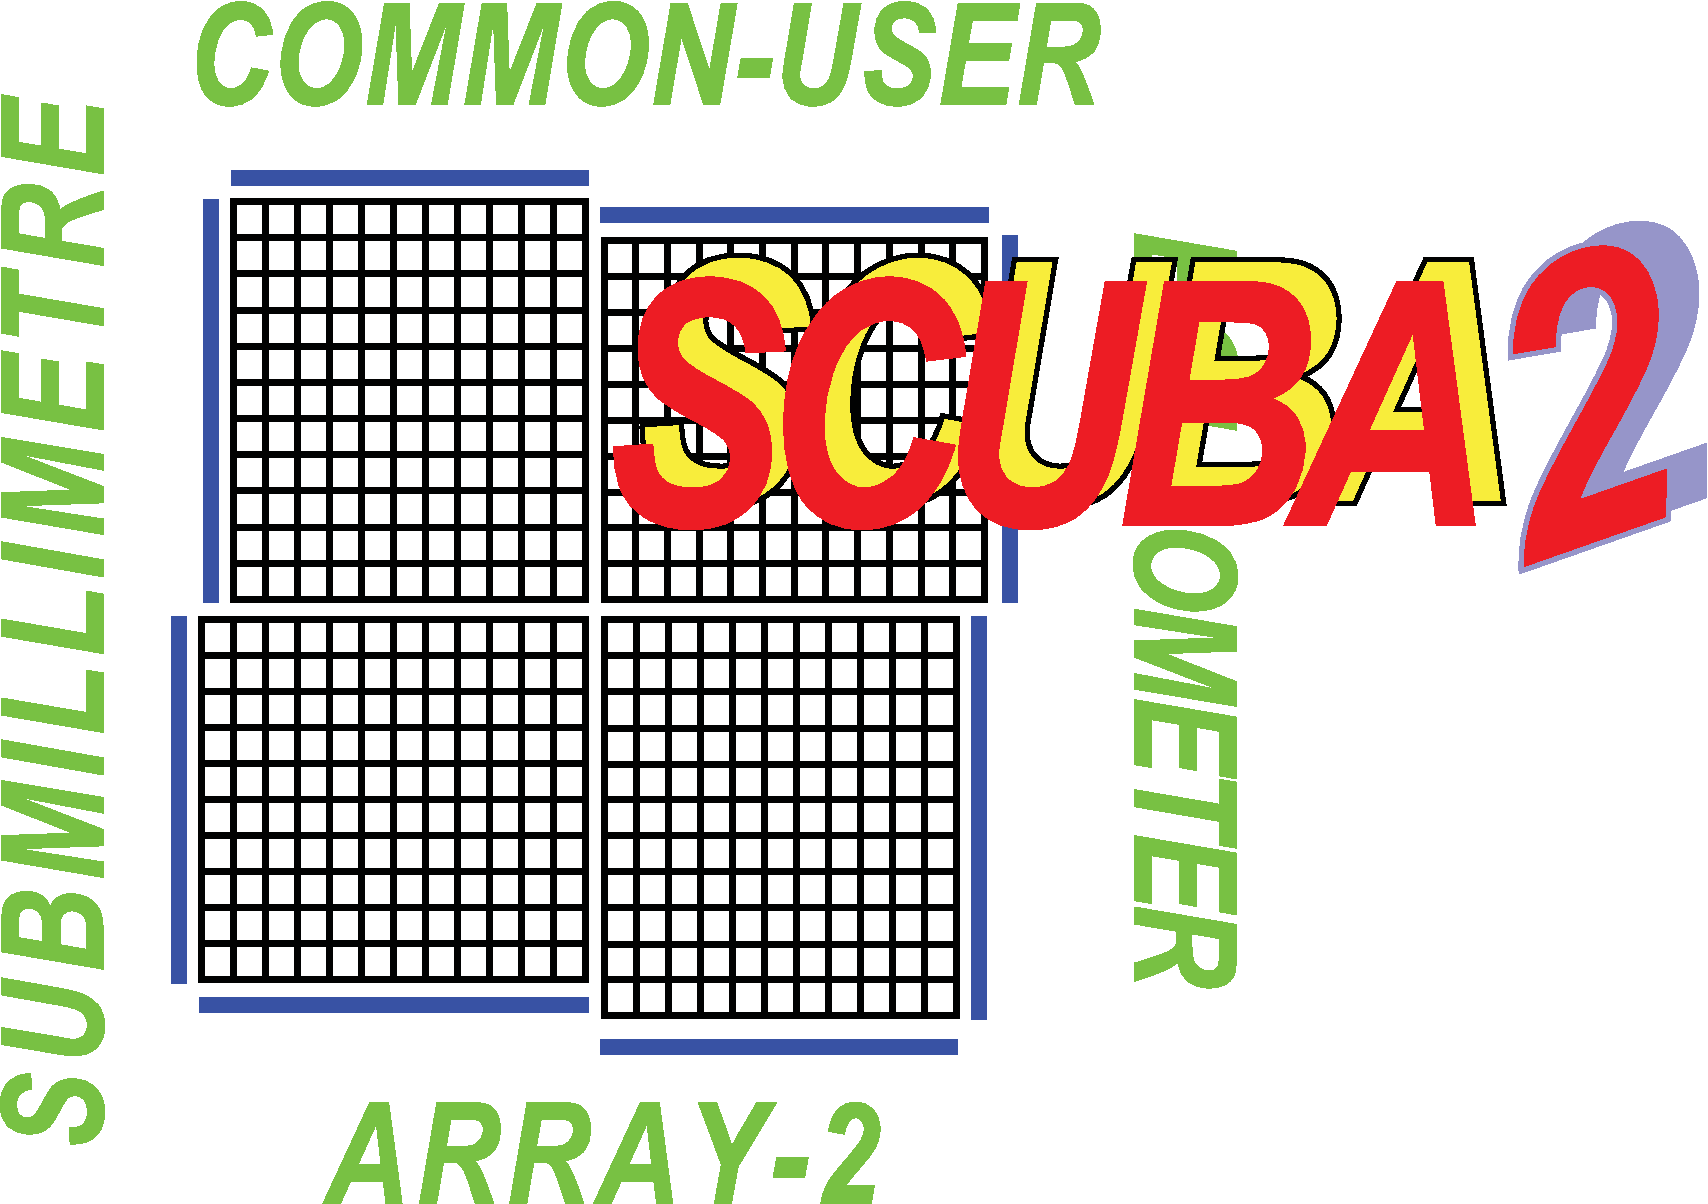
\includegraphics[width=0.7\textwidth]{sc21_s2logo}}


\newcommand{\minipageclear}{%
\begin{minipage}[c]{1.0\linewidth}\end{minipage}}

\begin{document}
\scfrontmatter

\newcommand{\xparam}[2]{\hyperref[#1]{\param{#2}}}
\newcommand{\setparam}[3]{\xparam{#1}{#2}\param{~=~#3}}

\newcommand{\jsageneric}{\htmladdnormallink{\file{dimmconfig\_jsa\_generic}}
{https://raw.githubusercontent.com/Starlink/starlink/master/applications/smurf/examples/dimmconfig_jsa_generic.lis}}

\newcommand{\brightextended}{\htmladdnormallink{\file{dimmconfig\_bright\_extended}}
{https://raw.githubusercontent.com/Starlink/starlink/master/applications/smurf/examples/dimmconfig_bright_extended.lis}}

\newcommand{\brightcompact}{\htmladdnormallink{\file{dimmconfig\_bright\_compact}}
{https://raw.githubusercontent.com/Starlink/starlink/master/applications/smurf/examples/dimmconfig_bright_compact.lis}}

\newcommand{\blankfield}{\htmladdnormallink{\file{dimmconfig\_blank\_field}}
{https://raw.githubusercontent.com/Starlink/starlink/master/applications/smurf/examples/dimmconfig_blank_field.lis}}

\newcommand{\fixconvergence}{\htmladdnormallink{\file{dimmconfig\_fix\_convergence}}
{https://raw.githubusercontent.com/Starlink/starlink/master/applications/smurf/examples/dimmconfig_fix_convergence.lis}}

\newcommand{\fixblobs}{\htmladdnormallink{\file{dimmconfig\_fix\_blobs}}
{https://raw.githubusercontent.com/Starlink/starlink/master/applications/smurf/examples/dimmconfig_fix_blobs.lis}}



% Acronyms section
\Acronyms

\begin{table}[h!]
\begin{tabular}{ll}
\textbf{CADC}   & Canadian Astronomy Data Centre\\
\textbf{CSO}    & Caltech Submillimetre Observatory\\
\textbf{DIMM}   & Dynamic Iterative Map-Maker\\
\textbf{FCF}    & Flux Conversion Factor\\
\textbf{FITS}   & Flexible Image Transport System\\
\textbf{FWHM}   & Full-Width at Half-Maximum\\
\textbf{GAIA}   & Graphical Astronomy and Image Analysis Tool\\
\textbf{ITC}    & Integration Time Calculator\\
\textbf{JCMT}   & James Clerk Maxwell Telescope\\
\textbf{MSB}    & Minimum Schedulable Block\\
\textbf{NDF}    & Extensible N-Dimensional Data Format\\
\textbf{NEP}    & Noise Equivalent Power\\
\textbf{NEFD}   & Noise Equivalent Flux Density\\
\textbf{PSF}    & Point Spread Function\\
\textbf{PWV}    & Precipitable Water Vapour\\
\textbf{RMS}    & Root Mean Square\\
\textbf{SCUBA-2}& Submillimetre Common User Bolometer Array-2\\
\textbf{SMURF}  & Sub-Millimetre User Reduction Facility\\
\textbf{S/N}    & Signal-to-Noise ratio\\
\textbf{SQUID}  & Superconducting QUantum Interference Device\\
\textbf{STC-S}  & Space-Time Coordinate Metadata String Implementation\\
\textbf{SUN}    & Starlink User Note\\
\textbf{TES}    & Transition Edge Sensor\\
\textbf{WVM}    & Water Vapour radioMeter\\
\end{tabular}
\end{table}


\newpage
\chapter{Introduction}
\label{sec:intro}

% set up page numbers in arabic numerals and restart from 1
\renewcommand{\thepage}{\arabic{page}}
\setcounter{page}{1}

\section{This cookbook}

This guide is designed to instruct SCUBA-2 users on the best ways to
reduce and visualise their data using \starlink\ packages:
\smurf \cite{smurf}, \Kappa \cite{kappa}, \gaia \cite{gaia}, \oracdr\
\cite{oracdr} and \picard \cite{picard}.

This guide covers the following topics.
\begin{itemize}
\itemsep0em
\item \cref{Chapter}{sec:intro}{Chapter 1} -- Computer resources you'll need before getting started.
\item \cref{Chapter}{sec:s2}{Chapter 2} -- A description of SCUBA-2 and its observing modes.
\item \cref{Chapter}{sec:dimm}{Chapter 3}  -- An introduction to the Dynamic Iterative Map-Maker and
a description of the configuration files.
\item \cref{Chapter}{sec:pipe}{Chapter 4}  -- Instructions for using the \oracdr\ pipeline to reduce
your data ``the easy way'', along with details on data retrieved from the JSA.
\item \cref{Chapter}{sec:manual}{Chapter 5}  -- Instructions for using individual \smurf\ commands to
reduce your data ---  useful if you need extra flexibity.
\item \cref{Chapter}{sec:tweak}{Chapter 6}  -- Options for tailoring the configuration parameters to
improve your final map.
\item \cref{Chapter}{sec:eg}{Chapter 7}  -- Two worked examples covering a \htmlref{blank cosmology
field}{sec:cosmology} and a \htmlref{galactic field}{sec:bright_ex}.
\item \cref{Chapter}{sec:postprocess}{Chapter 8}  -- Post-processing reduction steps such as applying
the FCF, co-adding multiple maps and estimating the noise.
\item \cref{Chapter}{sec:raw}{Chapter 9}  -- SCUBA-2 Diagnostic Tools.


\end{itemize}

Throughout this document, a percent sign (\texttt{\%}) is used to
represent the Unix shell prompt. What follows each \texttt{\%} will be
the text that should be typed by the user to initiate the described action.

\section{\xlabel{computing} Before you start: computing resources}

Before reducing SCUBA-2 data using the Dynamic Iterative Map-Maker you should confirm you have
sufficient computing resources for your type of map.

We recommend the following:
\begin{table}[h!]
  \centering
  \begin{tabular}{ll}
    \hline
    \textbf{Reduction type} &\textbf{Memory} \\
    \hline
    Large maps (\textsc{pong})& 96 GB\\
    Small maps (\textsc{daisy})&32 - 64 GB\\
    Blank fields&32 - 64 GB\\
    \hline
  \end{tabular}
\end{table}

\subsubsection*{Why these recommendations?}

For large-area maps it is important to process a full observation in a
single chunk. See the text box on
\latexhtml{Page~\pageref{box:chunk}}{\htmlref{Chunking}{box:chunk}}\
for an explanation of chunking. For large maps, using normal map-maker
parameters a machine having 96\,GB is acceptable. It is important that
the memory is as fast as can be afforded, as RAM speed has a direct
linear effect on processing time given that the time-series data are
continually being funnelled through the CPU.

For blank-field surveys or smaller
regions of the sky you can usefully run the map-maker with less memory
and 32 to 64\,GB is reasonable depending on the specifics of your data
set. \textsc{smurf} is multi-threaded so multiple cores do help
although above eight cores the price/performance gains tend to drop
off.

If you have a very large machine (128\,GB and 24 cores) you may be able
to run two instances of the map-maker in parallel without chunking,
depending on the nature of the data. Use
the \envvar{SMURF\_THREADS}\footnote{\envvar{SMURF\_THREADS} should be
set to an integer value indicating the number of threads to be used by
each process.} environment variable to restrict each map-maker to half
the available cores.

\section{\xlabel{software}Before you start: software}

This manual uses software from the \starlink\ packages: \smurf\
\cite{smurf}, \Kappa\ \cite{kappa}, \gaia\ \cite{gaia}, \oracdr\
\cite{oracdr} and \picard\ \cite{picard}. Starlink software must be
installed on your system, and Starlink aliases and environment
variables must be defined before attempting to reduce any SCUBA-2
data.

\subsection{Data formats}
\label{sec:ndf}

Data files for SCUBA-2 use the Starlink N-dimensional Data Format (NDF,
see Jenness et al 2014\cite{ndf}), a hierarchical format which allows
additional data and metadata to be stored within a single file. \Kappa\
contains \xref{many commands}{sun95} {ap_classified}\ for examining and
manipulating NDF structures. The introductory sections of the \Kappa\
document (\xref{SUN/95}{sun95}{}) contain much useful information on
the contents of an NDF structure and how to manipulate them.

A single NDF structure describes a single data array with associated
meta-data. NDFs are usually stored within files of type ``\verb+.sdf+''.
In most cases (but not all), a single \verb+.sdf+ file will contain just
one top-level NDF structure, and the NDF can be referred to simply by
giving the name of the file (with or without the ``\verb+.sdf+'' prefix).
In many cases, a top-level NDF containing JCMT data will contain other
``extension'' NDFs buried inside them at a lower level. For instance, raw
files contain a number of NDF components which store observation-specific
data necessary for subsequent processing. The contents of these (and
other NDF) files may be listed with \HDSTRACEref. Each file holding raw
JCMT data on disk is also known as a `sub-scan'.

The main components of any NDF structure are:
\begin{itemize}
\item An array of numerical data (may have up to 7 dimensions - usually 3
for JCMT data);
\item An array of variance values corresponding to the numerical data
values;
\item An array holding up to eight boolean flags (known as ``quality
flags'') for each pixel;
\item World Coordinate System information;
\item History;
\item Data units
\item Other extensions items. These are defined by particular packages,
but usually include a list of FITS-like headers together with provenance
information that indicates how the NDF was created. Raw JCMT file also
include extensions that define the state of the telescope and instrument
at each time slice within the observation.
\end{itemize}

The \convert\ package contains commands \xref{\task{fits2ndf}}{sun55}{FITS2NDF} and
\xref{\task{ndf2fits}}{sun55}{NDF2FITS} that allow interchange between FITS
and NDF format.

\subsection{Initialising Starlink}
\label{sec:starinit}

The commands and environment variables needed to start up the required
Starlink packages (\smurf \cite{smurf}, \Kappa, \emph{etc.}) must first
be defined. For C shells (csh, tcsh), do:

\begin{terminalv}
% setenv STARLINK_DIR <path to the starlink installation>
% source $STARLINK_DIR/etc/login
% source $STARLINK_DIR/etc/cshrc
\end{terminalv}

before using any Starlink commands. For Bourne shells (sh, bash, zsh), do:

\begin{terminalv}
% export STARLINK_DIR=<path to the starlink installation>
% source $STARLINK_DIR/etc/profile
\end{terminalv}

\subsection{KAPPA and SMURF for data processing}
\label{sec:packinit}

The Sub-Millimetre User Reduction Facility, or \textsc{Smurf},
contains the Dynamic Iterative Map-Maker, which will process raw
SCUBA-2 data into images (see \smurfsun). \textsc{Kappa} meanwhile is
an application package comprising general-purpose commands mostly for
manipulating and visualising NDF data (see \kappasun). Before starting
any data reduction you will want to initiate both \textsc{Smurf} and
\textsc{Kappa}.

\begin{terminalv}
% smurf
% kappa
\end{terminalv}

After entering the above commands, you can access the help information
for either package by typing \texttt{smurfhelp} or
\texttt{kaphelp} respectively in a terminal, or by using the
\task{showme} facility to access the hypertext documentation. See
\cref{Section}{sec:help}{How to get help} for more information.



\begin{tip}
The .sdf extension on filenames need not be specified when running most
Starlink commands (the exception is \picard).
\end{tip}


\subsection{GAIA for viewing your map}

Image visualisation can be done with \gaia\ (see
\gaiasun). \textsc{Gaia} is an image and data-cube display and
analysis tool, which incorporates facilities such as source detection,
three-dimensional visualisation, photometry and the ability to query
and overlay on-line or local catalogues.
\begin{terminalv}
% gaia map.sdf
\end{terminalv}

Alternatively, the \Kappa\ package includes many command-line driven
visualisation tools - see Appendix ``\xref{Classified KAPPA
commands}{sun95}{cl_datadisplay}'' in SUN/95\footnote{Particularly useful is the
ability of \Kappa\ to divide the screen up into many pictures, displaying
a different plot in each one.}.

\subsection{ORAC-DR for running the pipeline}

The \oracdr\ Data Reduction Pipeline \cite{oracdr} (hereafter just
\textsc{Orac-dr}) is an automated reduction pipeline. \textsc{Orac-dr}
uses \smurf\ and \Kappa\ (along with other Starlink tools) to perform
an automated reduction of the raw data following pre-defined recipes
to produce calibrated maps.  The following commands initialise
\textsc{Orac-dr} ready to process 850\,$\mu$m and 450\,$\mu$m data
respectively.
\begin{terminalv}
% oracdr_scuba2_850
% oracdr_scuba2_450
\end{terminalv}
For more information on available recipes and intructions for running the pipeline
see \cref{Chapter}{sec:pipe}{The SCUBA-2 Pipeline}.

\subsection{PICARD for post-reduction processing}

\textsc{Picard} uses a pipeline system similar to \oracdr\ for
post-processing and analysis of reduced data. \textsc{Picard}
documentation can be found at
\href{http://www.oracdr.org/oracdr/PICARD}{\textsc{Orac-dr} web page},
or at \picardsun. All \textsc{Picard} recipes follow the same
structure and are run like so:
\begin{terminalv}
% picard -recpars <recipe_params_file> RECIPE <input_files>
\end{terminalv}
where \param{<recipe\_param\_file>} is a text file containing the
relevant recipe parameters. \param{RECIPE} is the name of the recipe
to be run (note the caps). The list of files to be processed is given
by  \param{<input\_files>}. These must be in the current directory or a
directory defined by the environment variable \envvar{ORAC\_DATA\_IN}. A
number of \textsc{Picard} recipes will be demonstrated in
\cref{Chapter}{sec:maps}{Reducing your data}.

Other command-line options include \texttt{-log xsf} where the log
file is written to any combination of the screen [\texttt{s}], a file
[\texttt{f}] or an X-window [\texttt{x}]. \texttt{s} or \texttt{sf} is
recommended as the recipes are short and the X-window automatically
closes upon completion.

You do not specify an output filename for \picard, instead the output
is generated by adding a recipe depending suffix to the input
filename. If there is more than one input file then the name of the
last file is used.

You can create a file which lists the input files to be passed to
\picard\ for processing. this file is read by \picard\ via the
Linux/Unix \task{cat} command. For example:

\begin{terminalv}
% picard -log s RECIPE_NAME `cat myfilestoprocess.lis`
\end{terminalv}

To execute the \task{cat} command you must enclose it in back
quotes. You must also include the \file{.sdf} extension on any files
passed to \picard.

\begin{tip}
  Unlike other Starlink packages, the .sdf extension must be included
  when supplying the names of Starlink data files to \textsc{Picard}.
\end{tip}

\begin{tip}
  If the environment variable \envvar{ORAC\_DATA\_OUT} is defined, any
  files created by \textsc{Picard} will be written in that
  location. Check there if new files are expected but do not appear in
  your working directory.
\end{tip}


\subsection{\xlabel{help}How to get help}
\label{sec:help}

\begin{table}[h!]
\begin{tabular}{p{2.3cm}|p{7.3cm}|p{5cm}}
\hline
\textbf{Help\newline command} & \textbf{Description} & \textbf{Usage}\\
\hline
\task{showme} & If you know the name of the Starlink document you want to view
                use \task{showme}. When run, it launches a new webpage or tab
                displaying the hypertext version of the document. &
\texttt{\%~showme~sun95}\\
\hline
\task{findme} & \task{findme} searches Starlink documents for a keyword. When
                run, it launches a new webpage or tab listing the results. &
                \texttt{\% findme~kappa}\\
\hline
\task{docfind} & \task{docfind} searches the internal list files for keywords. It then
                 searches the document titles. The result is displayed using the
                 Unix \task{more} command. & \texttt{\%~docfind~kappa}\\
\hline
Run routines with prompts & You can run any routine with the option
                            \texttt{prompt} after the command. This will
                            prompt for every parameter available. If you
                            then want a further description of any parameter
                            type  \texttt{?} at the relevant prompt. &
                            \texttt{\%~makemap~prompt~\newline\~\%~REF~-~Ref.~NDF~/!/$>$~?}\\
\hline
Google & A simple Google search such as ``\texttt{starlink kappa fitslist}''
will usually return links to the appropriatre documents. However, be
aware that the results may include links to out of date versions of the
document hosted at non-Starlink sites. Always look for results in
\texttt{"www.starlink.ac.uk/docs} (or \texttt{"www.starlink.ac.uk/devdocs}
for the cutting-edge development version of the document). & \\
\hline
\end{tabular}
\end{table}

\section{Processing options}

You have two options for processing your data:

\begin{enumerate}
\item running the automated pipeline (\textsc{Orac-dr}), or
\item performing each step manually.
\end{enumerate}

The pipeline approach is simpler and works well if you have a
lot of data to process.
Performing each step by hand allows more fine-tuned control of certain
processing and analysis steps, and is especially useful for refining
the parameters used by the map-maker. However, once the optimal
parameters have been determined, it is possible to pass them to the
pipeline to process other observations using the same configuration.
\cref{Chapter}{sec:dimm}{The Dynamic Iterative Map-maker
Explained} and \cref{Chapter}{sec:manual}{Running makemap Outside the
Pipeline} discuss the manual approach; to use the science pipeline,
skip straight to \cref{Section}{sec:pipe}{The SCUBA-2 Pipeline}.

The JCMT will produce pipeline reduced files for each observation and
group of repeat observations for each night. These are reduced using
the \oracdr\ pipeline with the recipe specified in the MSB.
\cref{Chapter}{sec:pipe}{The SCUBA-2 Pipeline} gives instruction on
retrieving reduced data from the \htmladdnormallink{JCMT Science
  Archive}{http://www3.cadc-ccda.hia-iha.nrc-cnrc.gc.ca/jcmt/} at
CADC.

\newpage
\chapter{\xlabel{scuba2_overview}SCUBA-2 Overview}
\label{sec:s2}
\section{\xlabel{scuba2}The instrument}


The Submillimetre Common User Bolometer Array-2 (SCUBA-2) is a
10,000-pixel bolometer camera. It has two arrays operating
simultaneously to map the sky in the atmospheric windows of 450 and
850$\mu$m. Each array is made up of four sub-arrays as shown in
\cref{Figure}{fig:arrays}{}.

\subsubsection*{How it works}
The SCUBA-2 bolometers are integrated arrays of superconducting
transition edge sensors (TESs) with a characteristic transition
temperature, $T_c$. In addition, each TES is ringed with a resistive
heater which can compensate for changes in sky power. The SCUBA-2
focal plane is kept at a base temperature slightly below $T_c$,
however a voltage is applied across each TES resistance to position
the bolometer at the transition temperature. From this point, any
increase of temperature on the bolometers (e.g. from an astronomical
signal) will increase the TES resistance and heat it up. This causes a
drop in current and therefore a drop in temperature making the system
self-regulating.

For properly performing bolometers, the change in current through the
TES is proportional to the change in resistance, with the response
calibrated using flat-field observations (described below). This
changing current generates a magnetic field which is amplified by a
chain of superconducting quantum interference devices (SQUIDs). This
induces a feedback current which is proportional to the current
flowing through the TES, and it is this feedback current that is
recorded during data acquisition.


\subsubsection*{Setups}

Before science data can be taken the system must be optimised. These
`setups' are performed after slewing to the azimuth of the source,
where the SQUID, TES and heater biases are set to pre-determined
nominal values, in order to position the bolometers in the middle of
the transition range.

\subsubsection*{Flat-field}

 The shutter then opens onto the sky, and
as it does so the gradual increase in sky power hitting the array is
compensated for by a decrease in the resistive heater power via a
servo loop designed to keep the TES output constant. This acts to keep
the bolometers positioned at the centre of the transition range and is
known as \textbf{heater tracking}.

The responsivity of the bolometers will change slightly between the
dark and the sky; therefore, once the shutter is fully open a fast
\textbf{flat-field} observation is carried out to recalibrate them.
\textbf{A flat-field measures the responsivity of each bolometer to
changing sky power}. It does this by utilising the resistance heaters
which are ramped up and down around the nominal value. The change in
current through the TES is then recorded for each bolometer giving a
measure of its responsivity. The flat field solution is then the
inverse linear gradient of the current as a function of heater power.

At this point bolometers with responsivities above or below a
threshold limit are rejected, along with bolometers that display a
non-linear response or have a poor S/N. A second flat-field is
performed at the end of an observation so bolometers whose
responsivity has changed over the course of the observation can be
flagged.

For full details of the array setup and operation see Holland et al.
(2013) \cite{s2main}.

\begin{figure}[t!]
\begin{center}
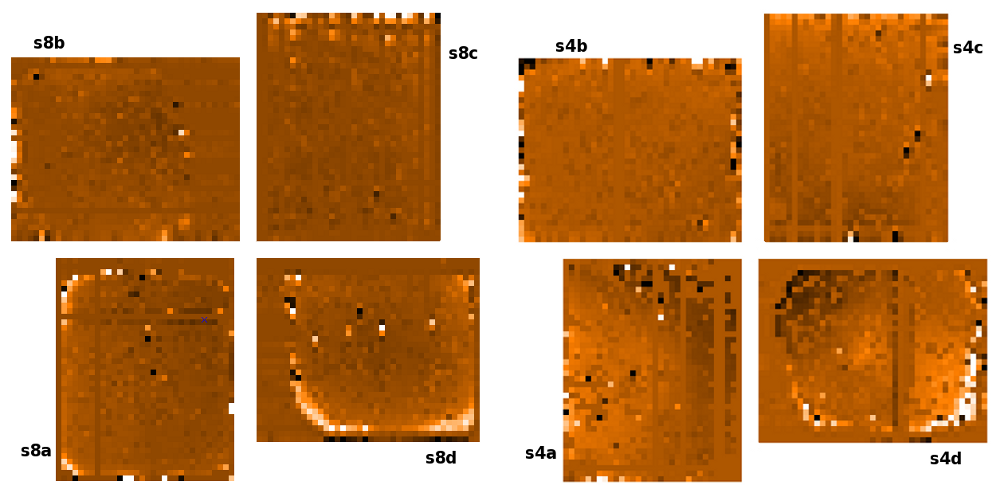
\includegraphics[width=0.8\linewidth]{sc21_arrays}
\label{fig:arrays}
\caption[The physical layout of the arrays at each wavelength]{
  \small The layout of the arrays at 850$\mu$m (left) and
  450$\mu$m (right). The labels denote the name assigned to each
  sub-array. Raw data files are generated separately for each sub-array
  and must be co-added. This figure was made by running
 \wcsmosaic\ on a raw sub-scan from each sub-array.
}
\end{center}
\end{figure}

\section{\xlabel{obs_modes}Observing modes}
\label{sec:mmodes}

Two observing modes are offered for SCUBA-2: \textsc{daisy} and
\textsc{pong}. As the bulk of \mbox{SCUBA-2} observing involves
large area mapping, both observing modes are scan patterns. Your
choice depends on the size of the area you wish to map, where you
would like your integration time concentrated and the degree of
extended emission you wish to recover.


\begin{aligndesc}

\item[\textbf{PONG}] A \textsc{pong} map is the scan strategy for
  covering a large area. The default options allow for three
  sizes---900\,arcsec, 1800\,arcsec and 3600\,arcsec. A single
  \textsc{pong} map is a square of these dimensions and the telescope
  fills in the square by bouncing off the edge of the area. To ensure
  an even sky background it is recommended a minimum of three, but
  preferably more than five, \textsc{pong} maps are included in a
  single observation with a rotation introduced between each one. In
  this way a circular pattern is built up, (see the lower right-hand
  panel of \cref{Figure}{fig:scan}{graphic below}), with a diameter
  equal to your requested map size.

  To recover large-scale extended structure you are advised to use
  larger \textsc{pong} maps which scan at a higher rate. This option
  is preferable to tiling multiple smaller maps. Ultimately it is the
  size of the SCUBA-2 field-of-view that determines the sensitivity to
  large-scale structure.

\item[\textbf{DAISY}] \textsc{daisy} maps are the option for
  point-like or compact sources ($<$3~arcmin) by maximising the
  exposure time on the centre of the image. The telescope moves at a
  constant velocity in a `spirograph' pattern that has the advantage
  of keeping the source on the array throughout the observation. This
  is shown in the top panel of \cref{Figure}{fig:scan}{the figure
    below}. While the central $<$3~arcmin has a uniform background noise,
    \textsc{daisy} maps cover a circular area of diameter of 12~arcmin.

\end{aligndesc}

\textbf{Should I use a \textsc{daisy} or a 15-arcmin \textsc{pong}?}  A 
common issue is that a pong900 is used when possibly 
a \textsc{daisy} would have been better, given that the latter is much faster and employs a significant 
exposure time out to a diameter of 12~arcmin. The numbers break down as follows:

\begin{figure}
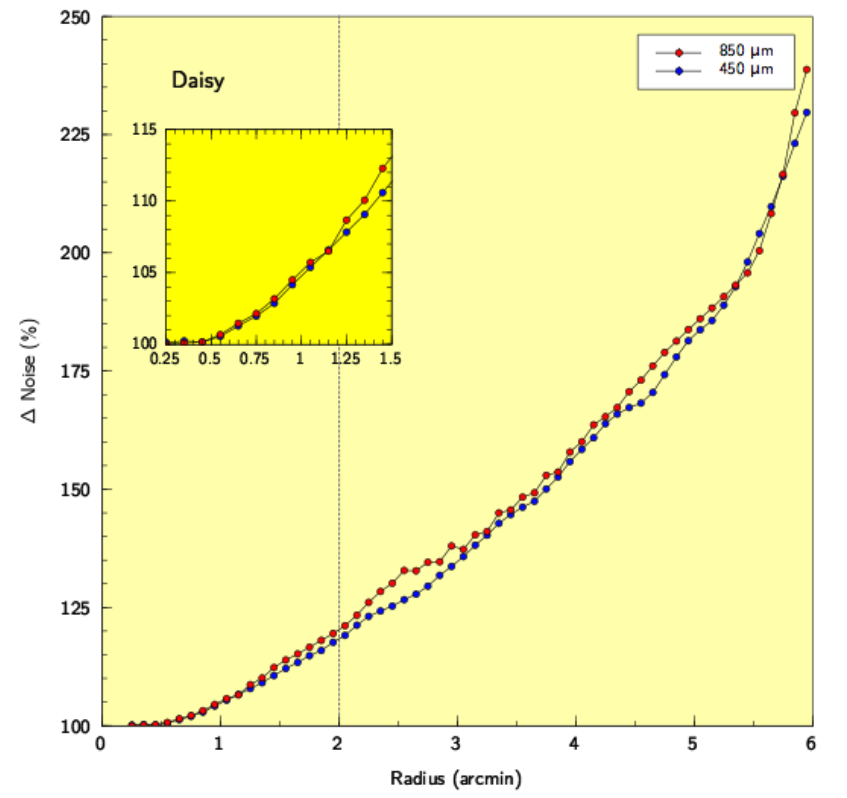
\includegraphics[width=0.47\linewidth]{sc21_DaisyRadProf.png}
\hspace{3mm}
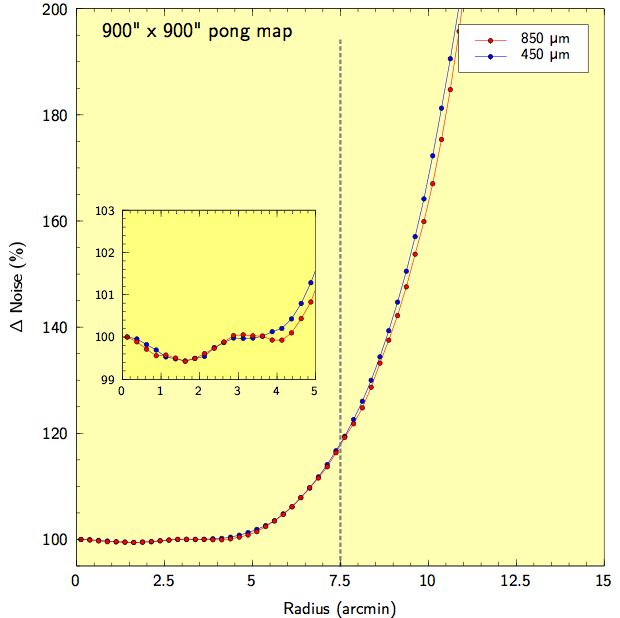
\includegraphics[width=0.445\linewidth]{sc21_Pong900RadProf.png}
\caption[Radial noise profiles for \textsc{Daisy} and \textsc{pong} maps.]{The
radial noise profiles for a \textsc{daisy} and \textsc{pong900} map. For the same integration time, the rms in the center ($<$3~arcmin) of a \textsc{daisy} will be more than twice as good as in a \textsc{pong900}. Out to a radius of $\sim$5.5~arcmin, the noise will still be below the \textsc{pong900} target noise.}
\label{fig:PongDaisyRadProf}
\end{figure}

\vspace{5mm}

\textit{For the same integration time}, the rms in the center ($<$3~arcmin) of a Daisy will be more than twice as good as in a pong900. Out to a radius of $\sim$5.5~arcmin, the noise will still be below the pong900 target noise. Beyond this radius the noise will exceed the target noise, but that is also the case for the pong900 (see the radial profiles in
\cref{Figure}{fig:PongDaisyRadProf}{}).

\vspace{5mm}

I.e. the trade-off is between a flatter and slightly larger map (pong900) and a somewhat smaller but much deeper map in the center with a distinct noise gradient across the field (\textsc{daisy}).

\vspace{5mm}

Detection experiments may well be better off with Daisies, although statistical conclusions, such as number counts, may become more complicated. The same may be true for isolated (i.e. non-mosaicked) fields where one could ask if the negative impact of the noise gradient and a smaller field out-weigh the benefits of a deeper mapping across most of the image.

There are other possibilities, such as doing an initial exploratory \textsc{daisy} to the required depth in a 3~arcmin field (this can be done in less that 25\% of the time it takes for a \textsc{pong900}) and then proceed with pongs on the most promising candidate(s). \textsc{pong} and \textsc{daisy} fields can be combined. It may also be beneficial to use a pattern of offset \textsc{daisies} to mitigate somewhat for the more pronounced gradient or to better match the source morphology in the field.

\subsubsection*{Why these patterns?}

SCUBA-2 removes atmospheric noise in the data-processing
stage (Holland et al. 2013) \cite{s2main}. The power spectrum
of data taken by SCUBA-2 has a $1/f$ noise curve at lower frequencies. To
ensure astronomical signals are far away from this $1/f$ noise, fast
scanning speeds are required.

In order to disentangle persistent source structure from other
slowly varying signals (e.g. extinction, sky noise, $1/f$ noise), the
scan pattern must pass across each region of the map from different
directions (hour angles) and at different times. The scan patterns themselves, along
with the associated parameters (velocity and scan-spacing), have been
designed and optimised to meet both these criteria. \textsc{daisies},
\textsc{pong900}, \textsc{pong1800}, and \textsc{pong3600} have telescope
velocities of 155$^{\prime\prime}$/s, 280$^{\prime\prime}$/s, 400$^{\prime\prime}$/s,
and 600$^{\prime\prime}$/s, respectively.

\starfig{sc21_wayne_scan}{[t!]}{width=0.98\linewidth}{fig:scan}{%
  Illustration of the SCUBA-2 observing patterns}{%

  The top row shows a \textsc{daisy} and the bottom row shows a
  \textsc{pong}.  The left column shows the telescope track over a
  single rotation of the pattern.  The right column shows the telescope
  track after multiple rotations of the pattern.  The scan pattern for
  an observation can be visualised in this way with \topcat\ using the
  output from \jcmtstate.  See \cref{section}{sec:scan}{Displaying
  scan patterns} for more details.  Figure modified from Holland et al. (2013).
}


\section{The raw data}
\label{sec:rawdata}
A normal science observation will follow the following sequence.

\begin{enumerate}\itemsep-0.2em
\item Flat-field
\item Science scans
\item Flat-field
\end{enumerate}

The \param{SEQ\_TYPE} keyword in the FITS header may be used to
identify the nature of each scan (see
\cref{Section}{sec:fitsheader}{Headers and file structure}).  When you
access raw from the \htmladdnormallink{Science
  Archive}{http://www3.cadc-ccda.hia-iha.nrc-cnrc.gc.ca/jcmt/} you
will get all of the files listed above. Later when you reduce your
data using the map-maker you must include all the science files
\emph{and} the first flat-field.  The final flat-field is not
currently used.

Shown below is a list of the raw files for a single sub-array (in this
case s8a) for a short calibration observation. The first and last
scans are the flat-field observations,which occur after the shutter
opens to the sky at the start of the observation and closes at the end
(note the identical file size); all of the scans in between are
science.


\begin{terminalv}
% ls -lh /jcmtdata/raw/scuba2/s8a/20131227/00034
\end{terminalv}

\begin{terminalv}
-rw-r--r-- 1 jcmtarch jcmt 8.0M Dec 27 03:00 s8a20131227_00034_0001.sdf
-rw-r--r-- 1 jcmtarch jcmt  22M Dec 27 03:00 s8a20131227_00034_0002.sdf
-rw-r--r-- 1 jcmtarch jcmt  22M Dec 27 03:01 s8a20131227_00034_0003.sdf
-rw-r--r-- 1 jcmtarch jcmt  22M Dec 27 03:02 s8a20131227_00034_0004.sdf
-rw-r--r-- 1 jcmtarch jcmt  22M Dec 27 03:02 s8a20131227_00034_0005.sdf
-rw-r--r-- 1 jcmtarch jcmt 6.8M Dec 27 03:02 s8a20131227_00034_0006.sdf
-rw-r--r-- 1 jcmtarch jcmt 8.0M Dec 27 03:03 s8a20131227_00034_0007.sdf
\end{terminalv}

The SCUBA-2 data acquisition (DA) system writes out a data file every
30 seconds; each of which contains 22\,MB of data. The only exception
is the final science scan which will usually be smaller (6.8\,MB in
the example above), typically requiring less than 30 seconds of data
to complete the observation.

\textbf{Note:} All of these files are written out eight times, once
for each of the eight sub-arrays.

The main data arrays of each file are cubes, with the first two
dimensions enumerating bolometer columns and rows within a sub-array,
and the third time slices (sampled at roughly 200\,Hz).

A standardised file naming scheme is used in which each file name starts
with the sub-array name, followed by the UT date of the observation in
the format \texttt{yyyymmdd}, followed by a five-digit observation
number, followed by the sub-scan number. The name ends with the standard
suffix \texttt{.sdf} used by all Starlink data files. For instance, the files
listed above hold data from the s8a sub-array for observation 34 taken on
27th December 2013.

\subsubsection*{Units}

Raw SCUBA-2 data come in uncalibrated units. The first calibration
step is to scale the raw data to units of picowatts (pW)
by applying the flat-field solution. This step is performed internally
by the map-maker but can be done manually when examining the raw
data---see \cref{Section}{sec:concat}{Concatenate \& apply a
  flat-field}.

The second step is to scale the resulting map by the flux conversion factor
(FCF) to give units of janskys. When running the
\textsc{Orac-dr} pipeline this is done automatically.
% STM: We are now encouraging users to stick with the nominal FCF values since there can be a significant
% variation over short timescales throughout the night. The long-term trends are, therefore, more robust, rather
% than picking one or two calibrator observations on a given night that may be affected by a variety of factors.
% Keeping this in mind, I am commenting out the lines below: 
%However it is good to check that the FCF value applied to your data is sensible.
%Checking FCF's must be done manually, instructions for this is
%given in \cref{Section}{sec:own_fcf}{Determining your own Flux conversion
%  factors}.



\newpage
\chapter{\xlabel{dimm}The Dynamic Iterative Map-Maker Explained}
\label{sec:dimm}

The Dynamic Iterative Map-Maker, hereafter just referred to as the
map-maker is the tool you will use to produce SCUBA-2 maps, and is
implemented by the \smurf\ \makemap\ command. It performs
all pre-processing steps to clean the data, followed by solving for
multiple signal components using an iterative algorithm, and binning
the resulting time-series data to produce a final science map.

The \makemap\ command can be invoked in two ways: 1) directly by typing
``\texttt{makemap}'' in response to a unix shell prompt (see
\cref{Chapter}{sec:manual}{Running the iterative map-maker}), or 2)
indirectly as part of an ORAC-DR recipe (see
\cref{Chapter}{sec:pipe}{The SCUBA-2 Pipeline}).

This chapter describes how the map-maker produces a science image
from raw SCUBA-2 data. It should be considered essential reading as it
provides an understanding of how your reduced image was produced. This is
particularly true if you wish to modify the default map-maker parameters.
\color{red}\textbf{ If you prefer to jump straight in to the data reduction go
to \cref{Chapter}{sec:pipe}{The SCUBA-2 Pipeline}.}\color{black}


\section{\xlabel{dimm_theory}How it works}

The map-maker works by producing individual models of the various
components that make up the signal recorded by each bolometer, one
component being the required astronomical signal.  It models and removes
each of the other components in order of decreasing magnitude, ultimately
leaving just the astronomical signal plus residual noise.  The modelled
components are listed in \cref{Table}{tab:mods}{tabulated} and described
more fully in \cref{Section}{sec:models}{The individual models}.

\textbf{A \emph{configuration file} should usually be supplied when
running \makemap directly.} This file holds a set of parameter values
that control all aspects of the map-maker, including details of the
pre-processing steps, which model components to include, parameters that
control the determination of each model, and the stopping (or
convergence) criteria. If no configuration file is supplied when running
\makemap\footnote{\emph{i.e.} you include ``\texttt{config=def}'' on the
\makemap\ command line.}, a set of default parameter values will be used.
There are a great number of these parameters, but fortunately not all of
them are of interest to the typical user. \cref{Appendix}{app:parameters}{}
documents the parameters you are more likely to find of interest,
including the default value that is assigned to each parameter if you do
not give it a value in your configuration file.  For a full list of all
available parameters, see the appendix \xref{``Configuration Parameters''}
{sun258}{par_full} within \xref{SUN/258}{sun258}{}.

It is possible to create a map without supplying a configuration file to
\makemap\ (\emph{i.e.} leaving all configuration parameters set to their default
values - ``\texttt{config=def}'' when running \texttt{makemap}) but it is not
recommeneded since it will not give optimal results
for your particular observation. For this reason, specialised
configuration files have been developed which are tailored to different
science goals, be they detecting faint galaxies or mapping large
molecular clouds. A description of these specialised configuration files
can be found \cref{in Section}{sec:config}{here}.

Note, when using the pipeline to create a map, rather than running
\makemap\ directly, the pipeline will always use a configuration file ---
one of the standard configuration files will be used if none is specified
by the user.

\section{The reduction step-by-step}
\label{sec:algorithm}

This section describes the basic map-making process used by the
default configuration.  It may be modified in many ways by supplying a
configuration file containing alternative parameter values.

\cref{Figure}{fig:dimm}{The graphic below} shows the flow chart of the
basic map-making process. It is divided into two sections: the pre-processing
stage where the data are cleaned, then the iterative stage where the different
models are subtracted, a sky map created and the convergence checked.


\begin{enumdesc}
\item[Initial cleaning and down-sampling]
  The separate raw data files are first concatenated into a single time
  series for each sub-array (if possible --- see \latexhtml{the description
  of \emph{Data Chunking} on Page~\pageref{box:chunk})~}{\htmlref{Data
  Chunking)}{box:chunk}} and have the flat-field from the associated
  fast-flat scans applied to calibrate the bolometers.  This resulting
  time-series are in units of pW.

  These time-series are then re-sampled at a rate that matches the
  requested pixel size --- the equivalent to applying a low-pass filter.
  Down-sampling saves time and memory usage when running the map-maker,
  without loosing any significant information. The degree of
  down-sampling applied depends on how fast the telescope was moving
  during the observation, the requested pixel size. In general, slower
  scans will be more heavily down-sampled than faster scans, and fast
  scans may not be down-sampled at all.

  A number of cleaning steps are then run: bolometers that have unusually
  high noise levels are identified and excluded from further processing,
  any sudden steps in the base-line of each bolometer are identified and
  corrected, and a polynomial estimate of the base-line is removed from
  each bolometer.

\item[Iterative steps]

  Next comes the iterative stage. In each iteration, estimates are
  produced for each model component. These are removed from the cleaned
  time-series data and the remaining data values are binned into a map.
  However, in general, the presence of astronomical signal within the
  original time series will have upset the estimates of the \model{COM},
  \model{GAI} and \model{FLT} models, causing the final map to be
  inaccurate. But now that we have a map (albeit an inaccurate map), we
  can sample the map at the position of each bolometer value to get an
  estimate of the astronomical component within the original time-series
  data. We then remove this astronomical signal from the original
  time-series data and re-estimate the models. These new model estimates
  should be more accurate since they are not so heavily
  influenced by the astronomical signal. In turn, this allows us to
  create a more accurate map.  We repeat this process until the map does
  not change significantly with further iterations. Whilst not
  mathematically rigorous, we expect the process to converge because the
  astronomical signal is in general much smaller than any of the other
  components and so each iteration introduces a very small fractional
  change in the model estimates.

  Within each iteration, the first components to be modelled and removed
  are \model{COM} and \model{GAI}, which work together to calculate and
  remove the average signal template of all bolometers, allowing each
  bolometer to have an arbitrary gain and offset. In addition, the
  \model{GAI} model will flag as unusable any bolometer in which the
  signal looks very different to the common-mode.

  The next model
  (\model{EXT}) applies a multiplicative extinction correction to the
  data. Following this, the \model{FLT} model filters each bolometer
  time-stream independently to remove low frequencies that correspond
  to angular scales larger than 600\,arc-sec and 300\,arc-sec at
  450$\mu$m and 850$\mu$m, respectively.

  After these models have been removed, the AST model (\emph{i.e.} the
  estimate of the astronomical signal) produced by the previous iteration,
  is added back onto the remaining time-series data\footnote{This step is
  omitted on the first iteration since no estimate of AST has yet been
  created.}, and the new values are binned up on the sky to produce a new
  estimate of the final science map.  Since many samples typically
  contribute to the estimate of the signal in a given pixel, the noise is
  greatly reduced compared with the time-series data. The variance of
  each map pixel value is determined from the spread of sample values
  that contribute to the pixel.  The value of this map at the position
  of each bolometer sample is then found. This forms the new \model{AST}
  model which is removed from the time-streams, leaving just the residual
  noise.

  The \model{NOI} model then measures the noise in the residual signals
  for each bolometer to establish weights for the data as they are placed
  into the map in subsequent iterations. This is only done on the first
  iteration. Subsequent iterations re-use the weights established on the
  first iteration.

\item[Checking convergence]

  Convergence is checked against the parameters detailed in the
  configuration file. Convergence is achieved either when the requested
  number of iterations has been completed, or when the mean change in the
  map pixel values is less than a specified fraction of a standard
  deviation (see parameter \xparam{MAPTOL}{maptol}).  If more iterations
  are required or (in the latter case) the map is still changing
  significantly, all the model --- \emph{except for AST} --- are added
  back onto the residuals, thus reconstructing the original time-series
  but without the astronomical signal.  This is the signal upon which the
  model estimates will be based on the next iteration.

\end{enumdesc}


\starfig{sc21_flow_dimm_blue}{}{width=0.78\linewidth}{fig:dimm}{
  Flowchart of the map-maker}{ A flow chart illustrating the dynamic
  iterative map-maker. Note that for each iteration the \model{AST}
  model is subtracted from the time-series leaving only those
  contributions to be fitted and removed.  }

For full details of the map-maker see \textbf{Chapin et al. (2013)}
\cite{mapmaker}.

\setlength{\extrarowheight}{3pt}
\begin{table}
\centering
\begin{tabular}{c|l}
\hline
\textbf{Model} &\hspace{0.2cm} \textbf{Description} \\
\hline
\model{COM}&\hspace{0.2cm} Common-mode signal\\
\model{GAI}&\hspace{0.2cm} Gains that scale each bolometer to the common-mode\\
\model{EXT}&\hspace{0.2cm} Extinction correction\\
\model{FLT}&\hspace{0.2cm} Filter that removes low frequencies\\
\model{AST}&\hspace{0.2cm} Astronomical signal\\
\model{NOI}&\hspace{0.2cm} Residual noise\\
\hline
\end{tabular}
\caption{\small Table adopted from Chapin et al. (2013). A detailed
explanation of each model is given in \cref{Section}{sec:models}{The individual models}.}
\label{tab:mods}
\end{table}

\raggedbottom

\begin{sltextbox}{Data Chunking}
  \caption{\label{box:chunk}}
  Chunking occurs when there is insufficient computer memory available
  for the map-maker to process all the time-series data together, or when
  there is a gap in the data (e.g.  from a missing sub-scan). In these
  cases, the map-maker divides up the time-series data into a number of
  ``chunks'' and produces a map from each chunk independently, before
  re-combining all the maps at a later stage to create the final map.
  Ideally you want your data reduced in a single chunk, however this can
  be unfeasible for large maps.

  The more data the map-maker processes at once, the better chance it
  has of determining the difference between sky signal and background
  noise.

  Information about chunking can be obtained in several ways:
  \begin{itemize}

  \item The screen output generated by \makemap\ will include one or more
  statements about chunking, such as:
  \begin{terminalv}
smf_iteratemap: Continuous chunk 1 / 1 =========
  \end{terminalv}
  The final number indicates the number of chunks being used (one in
  this case).

  \item The MEMLOW FITS header in the final map can be examined to
  determine if chunking occurred due to insufficient memory. For
  instance:
  \begin{terminalv}
% fitsval mymap memlow
FALSE
  \end{terminalv}
  indicates that the map in file \texttt{mymap.sdf} did not suffer from
  chunking as a result of low memory.

  \item The NCONTIG FITS header in the final map can be examined to
  determine if chunking occurred due to the supplied input data being
  discontiguous. For instance:
  \begin{terminalv}
% fitsval mymap ncontig
2
  \end{terminalv}
  indicates that the time-series data from which \texttt{mymap.sdf} was
  created was broken into two contiguous groups of samples. This
  indicates a potential problem with the data - the NCONTIG header
  should normally be one.
  \end{itemize}

  In \textsc{daisy} mode chunking is less of a concern as the entire
  map area is covered many times in the space of a single observation.

  For \textsc{pong} maps chunking is a bigger concern, with the
  maximum number of chunks that can be tolerated dependent on the
  number of map rotations. For example, a 40-minute \textsc{pong} map
  with eight rotations may get divided into three or four
  chunks. Although not ideal, this will mean that each point is still
  covered by two or three passes. Fewer passes than this however and
  the map-maker become less effective.

  Be aware that focus observations are intentionally dis-contiguous. If
  you attempt to make a map from a focus observation, it will be
  processed in several chunks no matter how much memory your computer has.
\end{sltextbox}

\section{\xlabel{models}The individual models}
\label{sec:models}

The list of models to be evaluated (and removed) by the map-maker, and
the order in which they are used during the iterative stage, is given by
the \xparam{MODELORDER}{modelorder} parameter in the configuration file.
These models are modular however, so their order may be changed. The
default model order is given below.

\begin{terminalv}
modelorder = (com,gai,ext,flt,ast,noi)
\end{terminalv}

The only configuration file not following this model order is the one tailored
for blank field maps which does not include a \model{FLT} model in the
iterative stage but instead includes an equivalent high-pass filter
as part of the cleaning stage (see \cref{Section}{sec:config}{Specialised
configuration files}).

Below is an introduction to each model. More complete descriptions of the
models and all the associated caveats can be found in Chapin et al.
(2013) \cite{mapmaker}. Details of each model are controlled by a set of
configuration parameters that begin with the name of the model. For
instance, all parameters related to the \model{COM} model will be of the
form ``\param{COM.xxx}''.

\begin{longtable}{c p{0.8\textwidth}}
  \hline
  \textbf{MODEL} & \multicolumn{1}{c}{\textbf{DESCRIPTION}}\\
  \hline
  \endhead
  \ifpdf
  \hline
  \endfoot
\fi
  COM& The \model{COM} model removes the common-mode signal
  (the signal that is common to all bolometers), the dominant
  contributor to this signal being the sky noise. It determines this
  by simply averaging over all bolometers for each time slice.
  Bolometers are flagged as bad, (and thus omitted from the final
  map), if they do not resemble the \model{COM} model seen by the
  majority of the other bolometers.

  Extended emission on a scale larger than the array footprint on the
  sky will contribute a signal indistinguishable from a common-mode
  signal. This puts an upper limit on the spatial scale of
  astronomical emission that can be recovered.\\
  \hline
GAI& \model{GAI} model works with \model{COM} in removing the
  common-mode signal. \model{GAI} consists of a time-varying scale
  and offset for each bolometer, which scales the \model{COM} model
  so that it resembles the original bolometer data as closely as possible.
  It is the scaled version of \model{COM} that is removed from the
  bolometer time-series.  In addition, the \model{GAI} model identifies
  any bolometers that looks very different to the common-mode signal, and
  flags them as unusable. \\
\hline
EXT& \model{EXT} applies the extinction correction. This is a
  time-varying scaling factor that is derived from the JCMT
  water-vapour radiometer. As it deals with 30-second chunks of data,
  this accounts for varying conditions over a long observation. For
  more details see \cref{Appendix}{app:cal}{SCUBA-2 data
    calibration}.\\
\hline
FLT& The \model{FLT} model acts on the Fourier transform of the
  bolometer data. High-pass (only allows \textit{higher} frequencies
  to pass) and low-pass (only allows \textit{lower} frequencies to
  pass) filters can be specified. These cut-off frequencies can either
  be specified directly in Hz, or as an angular spatial scale in
  arc-seconds that is subsequently converted into a frequency using
  the speed at which the telescope is moving. The most important role of
  this model is to apply a high-pass filter in order to remove the
  low frequency $1/f$ noise. Note that extended emission varies slowly
  over the array; it therefore appears at low frequencies and complicates
  the choice of a high-pass filter. A further discussion of this matter is
  given in \cref{Section}{sec:bright_ex}{Extended galactic sources}.\\
\hline
AST& The \model{AST} model is generated in conjunction with a
  science map. Hence, the position of \model{AST} in the model order
  indicates at what stage the astronomical image should be
  estimated. When the \model{AST} model is calculated, the first step is
  bin the residual time-series data into a map (using nearest-neighbour
  sampling). Following this, the map is projected back into the time
  domain (\emph{i.e.} sampled at the position of every bolometer sample)
  and removed as the \model{AST} model.\\
\hline
NOI& \model{NOI} should come last in the model order and
  calculates the RMS noise level in each bolometer.  It is only
  calculated on the first iteration. The same noise levels are then used
  on all subsequent iterations to weight the bolometer values when
  binning them into a map. Each bolometer may have a single noise estimate
  that remains fixed over the whole observation, or may have multiple
  noise levels, each of which relate to a different part of the observation.
  See parameters \xparam{NOI.BOX_SIZE}{noi.box\_size}
  and \xparam{NOI.BOX_TYPE}{noi.box\_type}. \\
\hline
\end{longtable}

Examples of the time traces for a single bolometer from these
models is shown in \cref{Figure}{fig:itercomp}{time-domain
components}. These traces cover a subset of an observation of the
secondary calibrator CRL~2688. You can clearly see the dominance of the
\model{COM} model which is removed first. The \model{FLT} model
stores the data removed by the high-pass filter. In the \model{AST}
model, CRL~2688 is clearly seen as positive spikes which appear when
the bolometer passes over the source. Finally, the residual signal
stored in \model{RES} is flat, indicating that most of the signal has
been successfully accounted for by the other model components.


\section{\xlabel{convergence}Stopping criteria}
\label{sec:converge}

The map-maker will stop processing either when the requested number of
iterations has been completed \textbf{OR} when the convergence
criterion specified in the configuration file is reached.


\textbf{Option 1: Fixed number of iterations}

Specifying the number of iterations in the configuration file is done
via the \xparam{NUMITER}{numiter} parameter. This is shown below for
\file{dimmconfig\_jsa\_generic.lis}.

\begin{terminalv}
numiter = -25
\end{terminalv}

A positive value for \param{numiter} means that the requested number
of iterations will be executed. A negative value, as in the example
above, indicates that no more than this number of iterations should be
performed, \emph{but} that it may stop at fewer if convergence
(according to the noise criterion below) has been achieved.

\textbf{Option 2: Convergence parameter}

The convergence criterion is set by the \xparam{MAPTOL}{maptol} parameter.

When running the map-maker, \texttt{maptol} gives the average
normalised change in the value of map pixels
between subsequent iterations. Convergence is reached when the  mean
change across all pixels is less than the parameter \param{maptol}.
It has units of the noise in the map, thus \texttt{maptol}$=$0.05 means
a mean change in pixel value of $<$0.05\,$\sigma$. This option has the
advantage of directly assessing the noise in the resulting map.

The map-maker displays the normalised change in pixel values between
iterations at the end of each iteration. This value typically drops
rapidly to begin with and then flattens out, decreasing increasingly
slowly.  The printed values can be inspected to check convergence is
proceeding as expected. Be aware that setting \texttt{maptol} to much
lower than 0.05 will dramatically increase the length of time needed to
produce the final map, and may possibly result in convergence never being
achieved.

If you wish to perform further checks on the progress of convergence
while running the map-maker, you can use the \xparam{ITERMAP}{itermap}
option. This causes the map created by each iteration to be dumped to
disk for inspection (see \cref{Section}{sec:tweak}{Tweaking the
configuration file}).

\begin{figure}
\begin{center}
  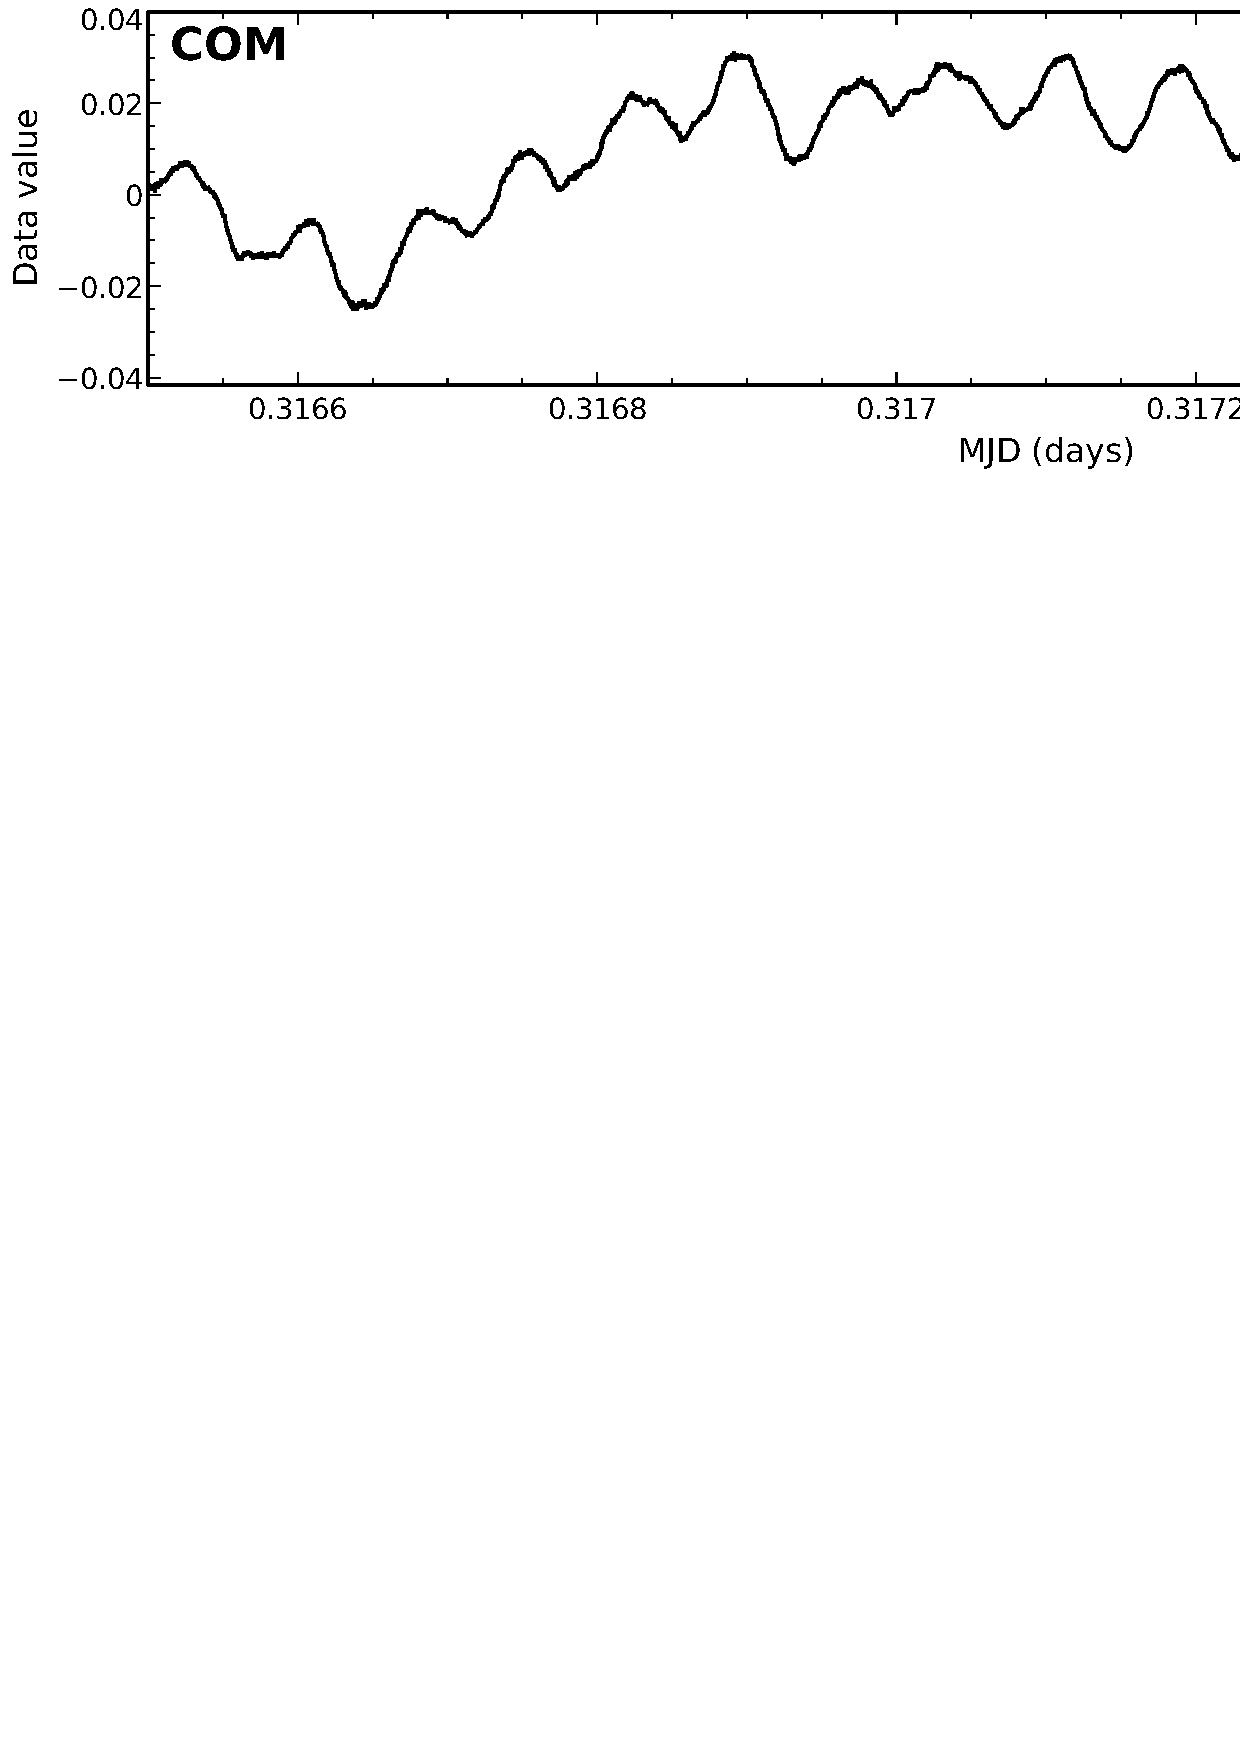
\includegraphics[width=\linewidth]{sc21_com} \\
  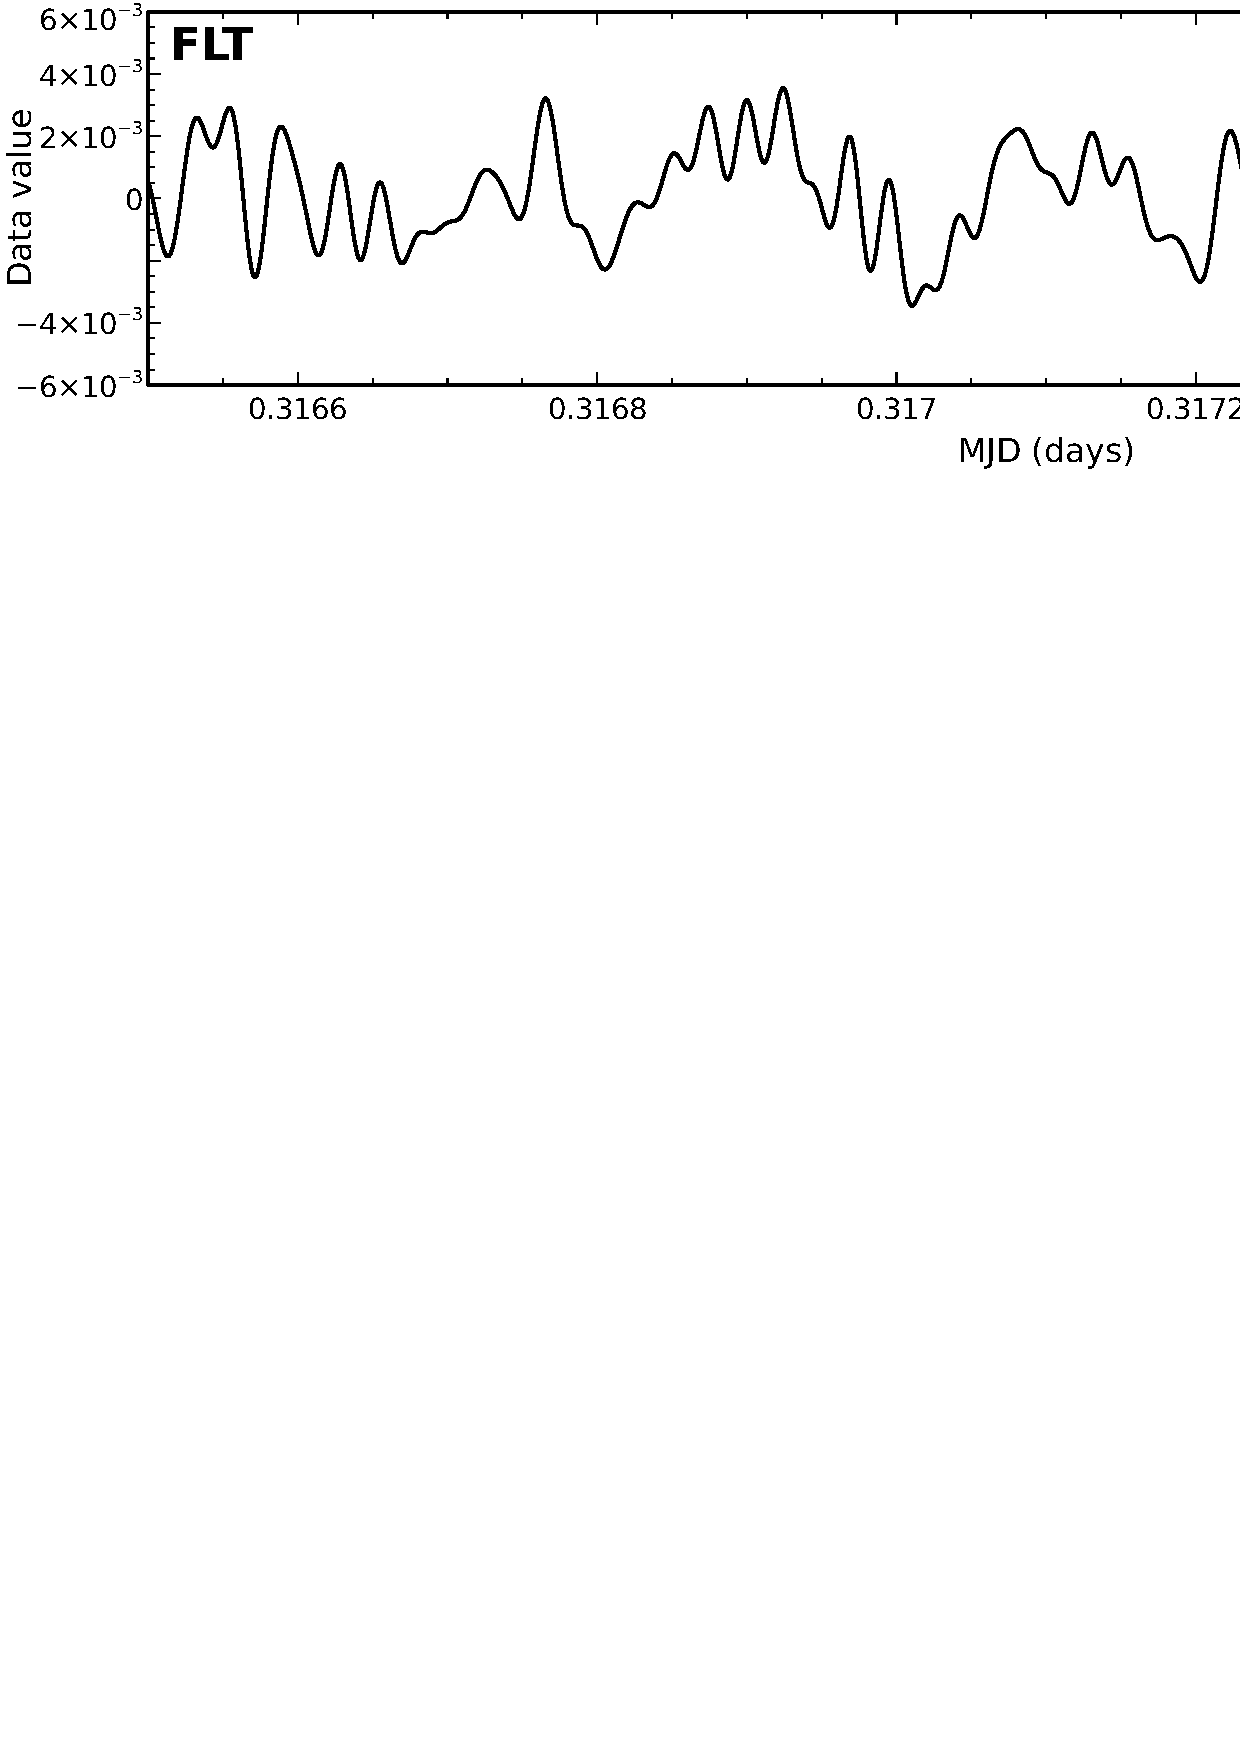
\includegraphics[width=\linewidth]{sc21_flt} \\
  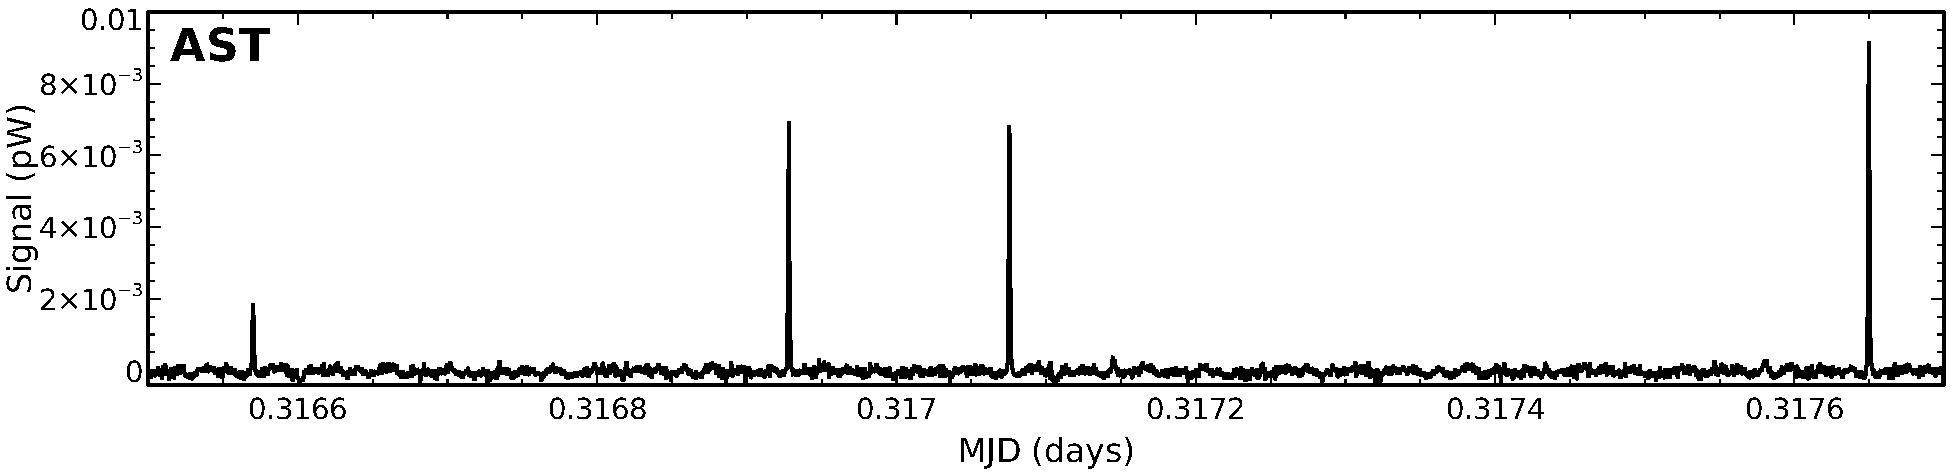
\includegraphics[width=\linewidth]{sc21_ast} \\
  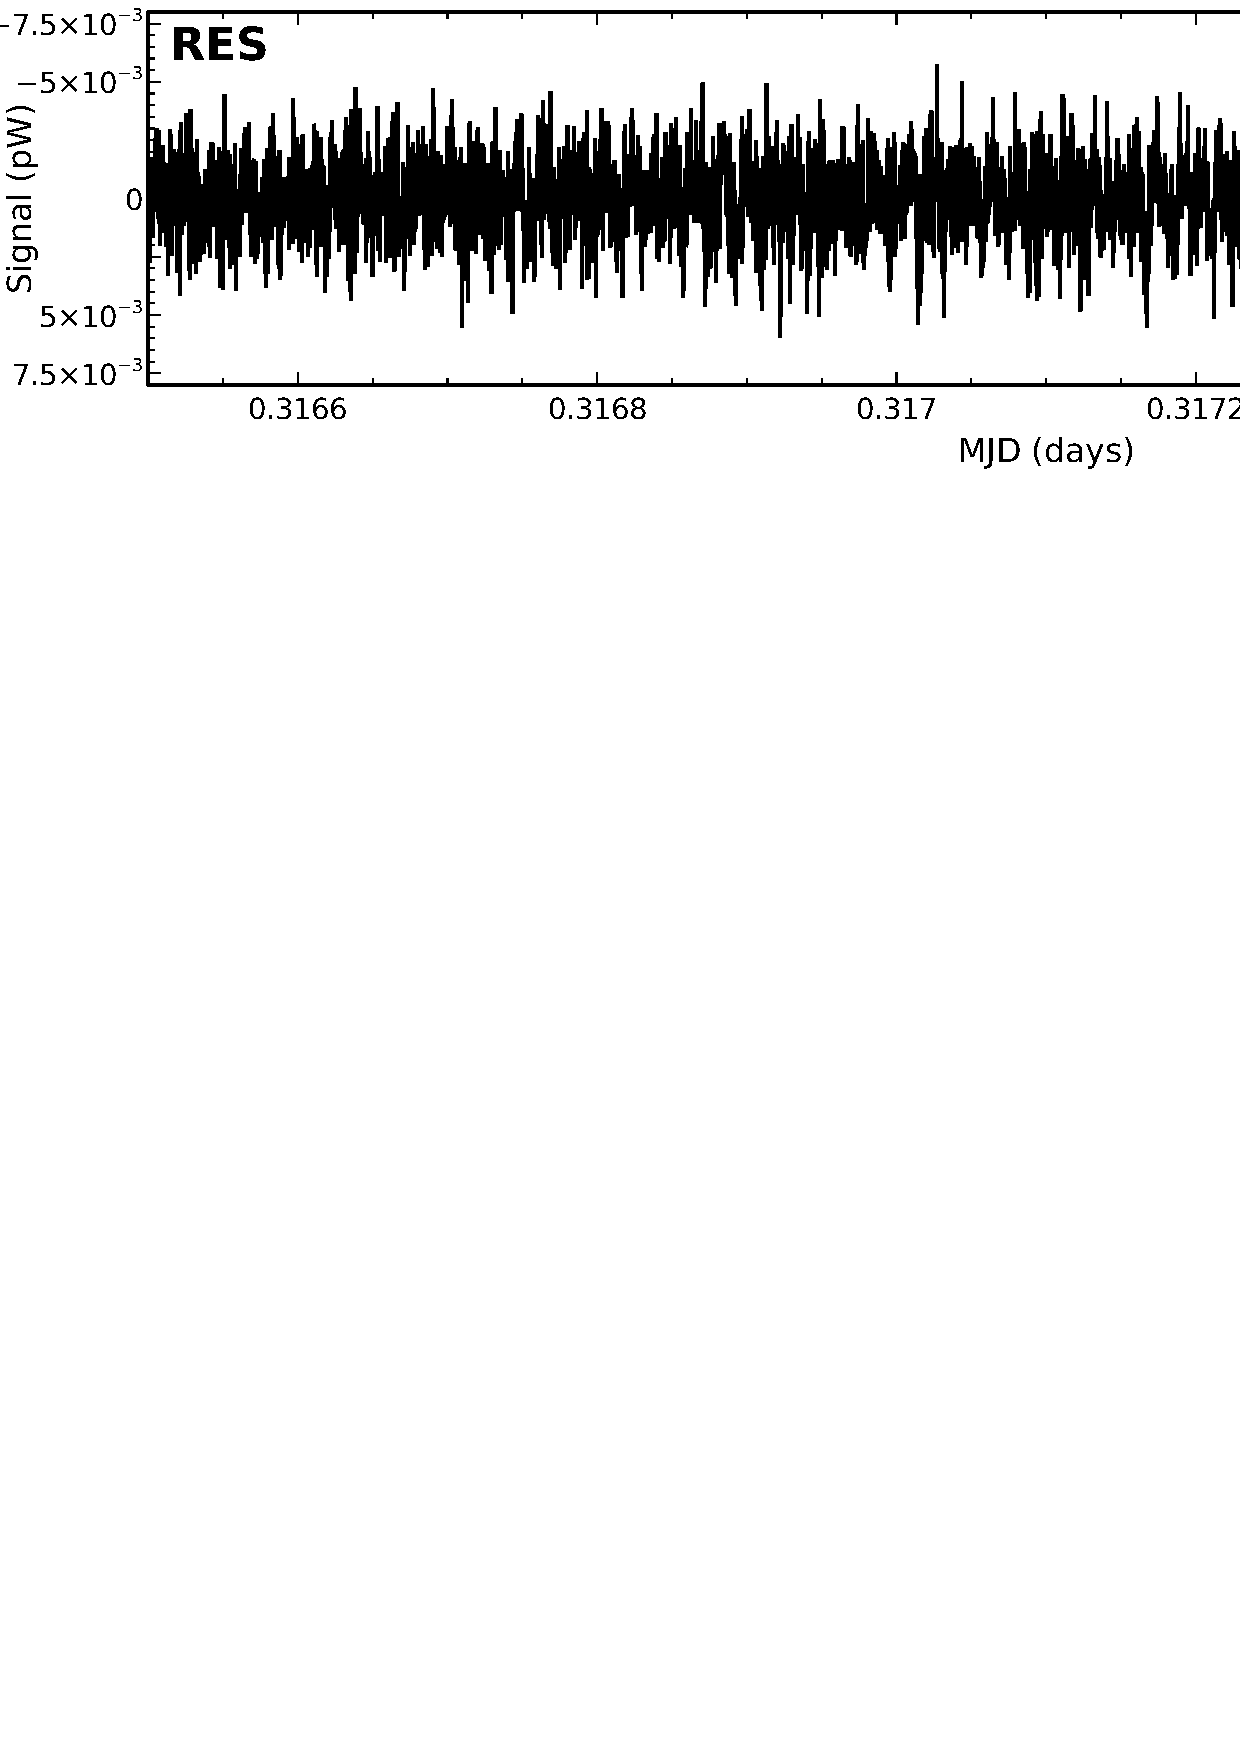
\includegraphics[width=\linewidth]{sc21_res} \\
\end{center}
\caption[Iterative models in the time domain]{\small These plots show
some of the models for a single bolometer, for part of an
observation of CRL~2688. From top to bottom: the \model{COM} model
containing signal common to all bolometers, the \model{FLT} model
containing residual low-frequency noise missed by \model{COM}, the
\model{AST} model with the astronomical signal showing as a positive
spike when this bolometer passes over the source, and the \model{RES}
model looking (as expected) like white noise.}
\label{fig:itercomp}
\end{figure}

\section{\xlabel{sec_masking}Masking}
\label{sec:masking}

The term \emph{masking} refers to the inclusion or exclusion of selected
bolometer samples from the estimate of specific models, based on the
positions of those samples within the output map. Masking can be applied
independently to the \model{AST}, \model{FLT} and \model{COM} models, as
described in the later sub-sections within this section.

A \emph{mask} is a selection of pixels within the output map. Normally
these pixels form one or more contiguous regions that enclose the areas
where significant sub-mm emission is expected (the ``source'' regions).
Pixels outside this mask are referred to as ``background pixels''. The use
to which such masks are put differs from model to model as described
later in model-specific sub-sections.

Masks fall into two broad categories:
\begin{itemize}

\item \textbf{dynamic masks} - these are masks that change shape from one
iteration to the next.

\item \textbf{static masks} - these are masks that retain the same shape
for all iterations.

\end{itemize}

Static masks are appropriate in cases where the areas containing significant
sub-mm emission are known in advance. If this is not the case, then the
mask needs to be based on evidence within the maps created at the end of
each iteration, resulting in the masks evolving from iteration to iteration
as the maps converge towards the final solution. Such \emph{dynamic} masks
have a potential problem  in that they can upset the convergence process by
introducing extra flexibility into the algorithm. For this reason, an
option is provided to freeze these masks after a fixed number of
iterations\footnote{Although by default masks are never frozen.}
(\emph{e.g.} see \xparam{AST.ZERO_FREEZE}{ast.zero\_freeze}) and this
is used within the specialist configuration file \fixconvergence\
described in \cref{Section}{sec:problem}{Configuration files for solving
specific problems}.

Each of the three models --- \model{AST}, \model{FLT} and \model{COM}
--- have an equivalent set of parameters to specify the masking (if any)
that should be used. Each set starts with the model name, followed by a
dot, followed by the parameter name. To enable masking, one or more of
these parameters needs to be set to a suitable value to define a mask, as
described below.

Static masks can be defined either as circles of specified radius,
centred on the source position (suitable for compact sources - see for
instance \xparam{AST.ZERO_CIRCLE}{ast.zero\_circle}), or by an external
image that uses special pixel values to indicate the source regions and
the background regions (suitable for extended sources - see for
instance \xparam{AST.ZERO_MASK}{ast.zero\_mask}). Within such ``external
masks'' all background pixels should be set to the Starlink \emph{bad} value
(see \xref{``Bad-pixel Masking''}{sun95}{se_badmasking} in SUN/95).
Pixels with any other value are treated as source pixels.
\cref{Section}{sec:maskbe}{Supplying an external mask} describes some
ways in which external masks can be generated.

Dynamic masks can be defined in several different ways:
\begin{enumerate}
\item By applying a simple threshold on the S/N ratio within the map
created at the end of each iteration (\emph{e.g.} see
\xparam{AST.ZERO_SNR}{ast.zero\_snr}).
\item By applying a simple threshold on the S/N ratio as above, and then
extending the resulting source regions down to a lower S/N value (\emph{e.g.}
see \xparam{AST.ZERO_SNRLO}{ast.zero\_snrlo}). This allows a low S/N
threshold to be used (which can sometimes help to avoid negative bowling
around the edges of extended sources) without introducing lots of isolated
pixels into the mask because of noise spikes in the map.
\item By applying a threshold on the number of bolometer samples falling
in each map pixel (\emph{e.g.} see \xparam{AST.ZERO_LOWHITS}
{ast.zero\_lowhits}). Because of the scanning strategy used with SCUBA-2
(see \cref{Section}{sec:mmodes}{Observing modes}), pixels near the edge of
the map will receive fewer bolometer samples than those near the centre,
and will therefore be noisier. Thus this scheme allows the noisy edges of
the map to be masked out. Whilst this is technically a dynamic mask ---
because the number of samples falling in each pixel could potentially change
from iteration to iteration --- in fact a mask based on hits per pixel
will usually only change very slightly from iteration to iteration.
\item By using an algorithm that automatically identifies features of a
given size in the map, similar to that used by the \textsc{Kappa}
\xref{\task{ffclean}}{sun95}{FFCLEAN} command (\emph{e.g.} see
\xparam{AST.ZERO_SNR_FFCLEAN}{ast.zero\_snr\_ffclean}). This can be a
useful alternative to simple S/N thresholding in cases where bright artificial
large-scale structures appear in the map. Such structures will result in
artificially large source regions in a simple S/N mask, which may in turn
cause the artificial structures to become even brighter and larger in
subsequent iterations. Using an \task{ffclean}-based mask instead will
restrict the mask to the brighter astronomical cores on top of such artificial
large-scale structures.
\end{enumerate}

Multiple masks can be used by selecting the appropriate configuration
parameters as described above. Whether the combined mask represents the
\emph{union} or \emph{intersection} of the individual masks is selected
using the parameters \xparam{AST.ZERO_UNION}{ast.zero\_union},
\xparam{FLT.ZERO_UNION}{flt.zero\_union} and \xparam{COM.ZERO_UNION}
{com.zero\_union}. By default, the union is used.



The masks used on the last iteration are stored in the \xref{\texttt{Quality}}
{sun95}{se_qualitymask} component of the NDF containing the output map.
A separate bit of the quality component is used for each model (\model{AST},
\model{FLT} or \model{COM}) that is being masked. These bits can be
viewed in various ways - see \cref{Section}{sec:maskshow}{Displaying masks}
and \cref{Section}{sec:itermaps}{Monitoring the map at the end of each
iteration}.

\begin{tip}
Be aware that the S/N ratio within individual map pixels depends on pixel
size --- larger pixels will have higher S/N ratios than small pixels.
Therefore masks based on a specific S/N threshold will grow or shrink in
area as a function of pixel size. As a rough rule, if you double the pixel
size, you should also double the S/N thresholds to get a mask that covers a
similar area of the sky.
\end{tip}

\subsection{\xlabel{sec_astmask}AST Masking}
\label{sec:astmask}
The iterative map-maker algorithm described earlier in this chapter
divides each cleaned bolometer value into four additive parts:
\begin{enumerate}
\item The common-mode signal (\model{COM}).
\item The low frequency background drift in each bolometer (\model{FLT}).
\item The astronomical signal (\model{AST}).
\item The left-over residual noise (\model{RES}).
\end{enumerate}

Whilst the value of each model is constrained to some extent by the
manner in which the model is calculated, there remains a large degree of
degeneracy in the algorithm. In other words, there are many different
ways in which each bolometer value can be divided up into the four values
listed above. For instance, any arbitrary change in the \model{AST} model
can be accommodated provided that equal and opposite changes are introduced
into the other model values so that the total value of all four components
remains the same.

The degeneracy between \model{COM} and \model{AST} is particularly
problematic, since it allows large scale features to appear in the map
(on the scale of the sub-array footprint) that are corrected for by equal
and opposite features in the \model{COM} model. Such features can appear
as gradients or ``saddles'' across the final map.

The purpose of masking the \model{AST} model is to apply an extra
constraint to the system to help break this degeneracy, and so avoid
these large-scale features. It functions by forcing the \model{AST} model
to zero at the end of each iteration for all samples that fall outside the
masked area on the sky (\emph{i.e.} samples that fall in the ``background''
areas of the map). Forcing the \model{AST} model to zero in this way means
that the \model{COM} model is more closely constrained.

Whilst this constraint is applied only in the background regions, its
effects are also felt part way into the source region because of the way in
which the \model{COM} model averages over a sub-array footprint. Thus source
regions that are much larger than a sub-array will still suffer from the
degeneracy between \model{COM} and \model{AST}, allowing arbitrary
large-scale background features to develop within the region, but these
features will become weaker as the edges of the mask are approached.

In order to avoid the final  map containing zero values in the background
region, it is necessary to avoid using \model{AST}-masking on the final
iteration. For this reason, by default one further iteration is performed ---
without \model{AST}-masking --- once the basic iterative algorithm has
converged (see \xparam{AST.ZERO_NOTLAST}{ast.zero\_notlast}).

All the configuration files supplied with \smurf\ use \model{AST}
masking, with the exception of \blankfield.

\subsection{\xlabel{sec_fltmask}FLT Masking}
\label{sec:fltmask}

The \model{FLT} model estimates and removes a low frequency background
from each bolometer time-stream. To do this it uses an FFT-based high-pass
filter. Ringing around sudden transients --- such as astronomical sources
--- is a natural consequence of all such filters, resulting in alternating
bright and dark rings around sources in the map. In most cases, the iterative
nature of the map-making algorithm eventually results in the rings
reducing to a much lower level, as more of the astronomical signal is removed
from the time stream on each iteration, causing the ring-inducing
transients to become weaker. However, this is not always completely
effective, and also slows down convergence.

For these reasons, it is often helpful to mask the \model{FLT} model.
This causes each bolometer time stream to be blanked out as the
bolometer passes over the source regions in the mask. Such blanked
sections are replaced by linear interpolation between the data on either
side of the blanked section. The effect of this is to remove the
transients that cause the ringing in the \model{FLT} model, and thus get
a better estimate of the low frequency background in each bolometer.

Such masking is most useful at the start of the iterative process,
before the bulk of the astronomical signal has been removed from the
time-streams. Indeed, if it is allowed to continue for too many iterations
it can cause its own problems that tend to slow down convergence. For
this reason, if \model{FLT} masking is used, it is (by default) limited
to two iterations ---  see \xparam{FLT.ZERO_NITER}{flt.zero\_niter}.

A difficulty with \model{FLT} masking is that the \model{FLT} model is
evaluated \emph{before} the map is made on each iteration. This means
that when the \model{FLT} model is evaluated on the first iteration,
there is no map available. This is not a problem if a static mask is
used, but if a dynamic mask is used, then it is not possible to calculate
the \model{FLT} mask on the first iteration (subsequent iterations will
create the mask on the basis of the map created at the end of the
previous iteration). This is a shame since \model{FLT} masking is most
beneficial on the first few iterations, whilst the bulk of the astronomical
signal is still present in the time streams. A scheme to get round this
problem is described in \cref{Section}{sec:skip}{Skipping the AST model}.

All the configuration files supplied with \smurf\ use \model{FLT}
masking, with the exception of \blankfield.

\subsection{\xlabel{sec_commask}COM Masking}
\label{sec:commask}

The value of the \model{COM} model at a specific time-slice is the mean
of all remaining bolometer values at that time slice. If the \model{COM}
model is masked, bolometer samples that fall within the source regions
defined by the mask are excluded from this mean, thus removing the bias
introduced into the mean by bright astronomical sources. This results in
the \model{COM} model more accurately representing the varying common-mode
background value at each time slice. This can help to reduce negative
bowling around sources in the map, and can help to reduce the amount of
data that is rejected as being too poorly correlated with the common-mode
signal.

\model{COM} masking has the same difficulty as \model{FLT} masking in that
the \model{COM} model is evaluated \emph{before} the map is made on each
iteration, and so it is difficult to use dynamic masks with \model{COM}
masking. However, the solution described in \cref{Section}{sec:skip}{Skipping
the AST model} can be used for \model{COM} masking as for \model{FLT}
masking.

Currently, none of the configuration files supplied with \smurf\ use
\model{COM} masking.

\section{\xlabel{sec_skip}Skipping the AST model}
\label{sec:skip}
As discussed in \cref{Section}{sec:masking}{Masking} - \model{FLT}
masking is most effective on the early iterations (particularly the very
first iteration). This is because the bulk of the astronomical signal is
still present in the time streams and is likely to cause bad ringing if
\model{FLT} masking is not used. However, since the \model{FLT} model
is evaluated before the map is made within each iteration, there is no map
available to use as the basis for a \model{FLT} mask on the very first
iteration.

One way to get round this is simply to use a static mask that does not
require a map to be available. However, this may not be possible -
particularly for extended sources where no \emph{a-priori} knowledge of the
source areas in the sub-mm may be available.

Another scheme is provided by the \xparam{AST.SKIP}{ast.skip}
configuration parameter. If \param{ast.skip} is set to a positive integer
$N$, the subtraction of the \model{AST} model from the time-series that
normally occurs at the end of each iteration is not performed on the
first $N$ iterations. This means that for the first $N$ iterations, the
time-series data remain unchanged, and consequently the models and the
resulting map are unchanged. Of itself, this does nothing useful --- it
merely delays the first useful iteration. However, when combined with
\model{FLT} masking, it can be very beneficial because it allows a mask
to be created \emph{before} the first ``real'' iteration occurs
(\emph{i.e.} the first iteration that subtracts off the \model{AST}
model). This means that the first ``real'' map will have far less
ringing around bright sources than would otherwise be the case.  This in
turn means that far fewer iterations are required to correct this ringing.

It is also possible to use \param{ast.skip} with \model{COM} masking, but
the benefits are no so noticeable as for \model{FLT} masking.

The default value for \param{ast.skip} is zero, but the \brightextended\
and \jsageneric\ configuration files supplied with \smurf\ both set
\setparam{AST.SKIP}{ast.skip}{5} (and also use \model{FLT} masking).

\section{\xlabel{config}Specialised configuration files}
\label{sec:config}

Maps made by the pipe-line using the
REDUCE\_SCAN recipe will use \file{dimmconfig\_jsa\_generic.lis} unless some
alternative configuration has been specified. This configuration file is
intended to provide a reasonably good map for all types of observations.
However, compromises have been made to reach that balance, the main one
being that some real extended structure is sacrificed in order to avoid
introducing artificial large scale structures.

Whilst \file{dimmconfig\_jsa\_generic.lis} is always a good place to start,
you will want to follow this up with a specialised configuration that will suit
your observation. A few specialised configuration files are supplied with
\smurf\ and can be found in \file{\$STARLINK\_DIR/share/smurf/}.

Note, any parameter for which no value is specified within the supplied
configuration will take on the default value listed in
\cref{Appendix}{app:parameters}{Configuration-parameter descriptions}.

Below is a description of each of the specialised configuration files.
The tables following each description list the parameters set by each file.
The files themselves are stored in \file{\$STARLINK\_DIR/share/smurf/} ---
they are simple text files and so can be inspected easily.

\subsection{dimmconfig\_jsa\_generic.lis}
The \jsageneric\ configuration file is designed to handle all science data. This is a good
configuration file to start with if you are unsure how to proceed with your
data reduction.  You may notice that elements of this configuration are
common to the other specialised configuration files.

This configuration is optimised to suppress the creation of artificial
large scale structure within the final map. Consequently, some real
extended emission may be lost if this configuration is used. This goal is
achieved by:

\begin{enumerate}

\item Setting
\xparam{FLT.FILT_EDGE_LARGESCALE}{flt.filt\_edge\_largescale}) to 200
arc-seconds so that the \model{FLT} model uses a  heavier than normal
filter.

\item Setting \xparam{COM.PERARRAY}{com.perarray} to 1, indicating that four separate
\model{COM} models should be used, one for each sub-array\footnote{By default, a single
\model{COM} model is used that represents the mean data value across all
four sub-arrays.}.

\item Using a mask to force the \model{AST} model to zero in the background regions
after each iteration (see parameters \xparam{AST.ZERO_SNR}{ast.zero\_snr}
and \xparam{AST.ZERO_SNRLO}{ast.zero\_snrlo} --- also see
\cref{Section}{sec:astmask}{AST masking}).

\end{enumerate}

In addition the S/N threshold for DC steps (\xparam{DCTHRESH}{dcthresh})
is relaxed from 25 in the default file to 100 to avoid problems bright
sources triggering the step detection algorithm.

The other major feature of this configuration is that the subtraction of
the \model{AST} model is skipped on the first five iterations. In
conjunction with the use of \model{FLT} masking, this helps to speed up
convergence and minimise dark rings around bright source (see
\cref{Section}{sec:skip}{Skipping the AST model}.

\latex{\renewcommand*\arraystretch{1}}
\begin{table}[h!]
\centering
\begin{tabular}{|p{6.5cm}p{6.5cm}|}
\hline
\multicolumn{2}{|l|}{\file{dimmconfig\_jsa\_generic.lis}}\\
\hline
\setparam{AST.SKIP}{ast.skip}{5}&\setparam{AST.ZERO_SNRLO}{ast.zero\_snrlo}{3}\\
\setparam{AST.ZERO_SNR}{ast.zero\_snr}{5}&\setparam{COM.PERARRAY}{com.perarray}{1}\\
\setparam{DCTHRESH}{dcthresh}{100}&\setparam{FLT.FILT_EDGE_LARGESCALE}{flt.filt\_edge\_largescale}{200}\\
\setparam{FLT.ZERO_SNRLO}{flt.zero\_snrlo}{3}&\setparam{FLT.ZERO_SNR}{flt.zero\_snr}{5}\\
\setparam{MAPTOL}{maptol}{0.01}&\setparam{NUMITER}{numiter}{-25}\\
\setparam{NOISECLIPHIGH}{noisecliphigh}{10.0}\\
\hline
\end{tabular}
\end{table}




\subsection{dimmconfig\_blank\_field.lis}

The \blankfield\ configuration is tuned for blank field surveys for which the goal
is to detect extremely low signal-to-noise point sources within otherwise
blank fields.

Applying a high-pass filter (\model{FLT}) on each iteration can result in
convergence problems when there is little or no signal in the
map. Instead, a single, harsher high-pass filter is applied as a
pre-processing step (corresponding to 200-arc-sec scales at both
450\,$\mu$m and 850\,$\mu$m). There are also more conservative cuts to
remove noisy/problematic bolometers. Only 4 (positive) iterations are
requested as there is no signal to confuse to models.

The option \xparam{COM.PERARRAY}{com.perarray}~=~1 requires the \model{COM} model to
be fit to each sub-array independently. This improves the overall fit
but with the loss of any structure on scales larger than a single
sub-array---not an issue for blank fields.

\cref{Figure}{fig:bfcompare}{The images below} shows the sharp
contrast in the output map between reducing data with the default
configuration file and using \file{dimmconfig\_blank\_field.lis}.

Blank-field maps commonly have a matched filter applied as part of the
post-processing to aid source detection (see
\cref{Section}{sec:mf}{Point-source detection}), however this is not
applied by the map-maker.

\begin{figure}[t!]
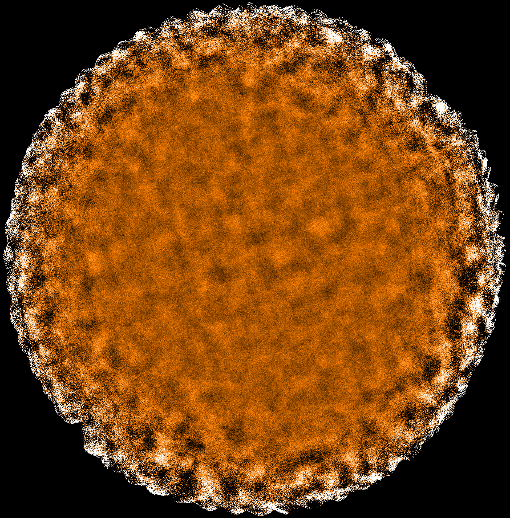
\includegraphics[width=0.47\linewidth]{sc21_cosmo1-def}
\hspace{3mm}
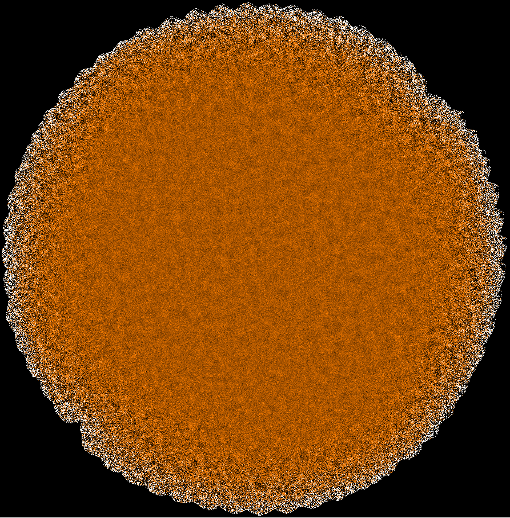
\includegraphics[width=0.47\linewidth]{sc21_cosmo1-bf}
\caption[Example map reduced with \file{dimmconfig\_blank\_field.lis}]{
    Maps of a deep cosmology field reduced with \textbf{(left)}
    default parameter values (\emph{i.e.} no configuration file) and
    \textbf{(right)} \file{dimmconfig\_blank\_field.lis} \label{fig:bfcompare}}.
\end{figure}



% The tildes around the equal sign are to ensure HTML table field is
% not wrapped after the parameter name.
\renewcommand*\arraystretch{0.95}
\begin{table}[h!]
\centering
\begin{tabular}{|p{6.5cm}p{7.0cm}|}
\hline
\multicolumn{2}{|l|}{\file{dimmconfig\_blank\_field.lis}}\\
\hline
\setparam{NUMITER}{numiter}{4}&\setparam{FILT_EDGE_LARGESCALE}{flt\_edge\_largescale}{200}\\
\setparam{SPIKETHRESH}{spikethresh}{10}&\setparam{MODELORDER}{modelorder}{(com,ext,ast,noi)}\\
\setparam{COM.PERARRAY}{com.perarray}{1}&\\
\hline
\end{tabular}
\end{table}




\subsection{dimmconfig\_bright\_compact.lis}

The \brightcompact\ configuration should be used for producing maps of
bright, isolated compact sources that are positioned at the centre of the
map (\emph{e.g.} calibrators).

The addition of the \xparam{AST.ZERO_CIRCLE}{ast.zero\_circle} parameter
is used to constrain the map to zero beyond a radius of 1\,arc-min from
the source centre (see \cref{Section}{sec:astmask}{AST masking}).  This
strategy helps with map convergence significantly, and can provide good
maps of bright sources, even in cases where scan patterns failed to
complete in full.

\xparam{COM.PERARRAY}{com.perarray} is set to 1 indicating that a \model{COM} model
should be fit separately for each sub-array. This is not advised for
extended sources as signal on scales larger than a single sub-array is
lost, but is fine for a compact central source. Likewise, the filtering
is tighter. The S/N threshold for DC steps (\xparam{DCTHRESH}{dcthresh}) is relaxed from
25 in the default file to 100 to avoid problems associated with bright sources.

The values of the parameters controlling the \model{COM} model are
modified to relax the test that compares each bolometer to the common
mode. This is because the algorithm that compares each bolometer to the
common-mode can be fooled by a bright compact source passing across
individual bolometers. Likewise the test for DC steps within each
bolometer baseline is also relaxes (parameter \xparam{DCTHRESH}{dcthresh}).

% The tildes around the equal sign are to ensure HTML table field is
% not wrapped after the parameter name.
\latex{\renewcommand*\arraystretch{0.95}}
\begin{table}[h!]
\centering
\begin{tabular}{|p{6.5cm}p{7.0cm}|}
\hline
\multicolumn{2}{|l|}{\file{dimmconfig\_bright\_compact.lis}}\\
\hline
\setparam{NUMITER}{numiter}{-40}&\setparam{FLT.FILT_EDGE_LARGESCALE}{flt.filt\_edge\_largescale}{200}\\
\setparam{COM.PERARRAY}{com.perarray}{1}&\setparam{FLT.ZERO_CIRCLE}{flt.zero\_circle}{(0.016666)}\\
\setparam{AST.ZERO_CIRCLE}{ast.zero\_circle}{(0.0166666666)}&\\
\setparam{NOISECLIPHIGH}{noisecliphigh}{10.0} & \setparam{DCTHRESH}{dcthresh}{100}\\
\setparam{COM.CORR_TOL}{com.corr\_tol}{7}& \setparam{COM.GAIN_TOL}{com.gain\_tol}{7}\\
\setparam{COM.GAIN_ABSTOL}{com.gain\_abstol}{5}& \\
\hline
\end{tabular}
\end{table}


\subsection{dimmconfig\_bright\_extended.lis}

\begin{figure}[t!]
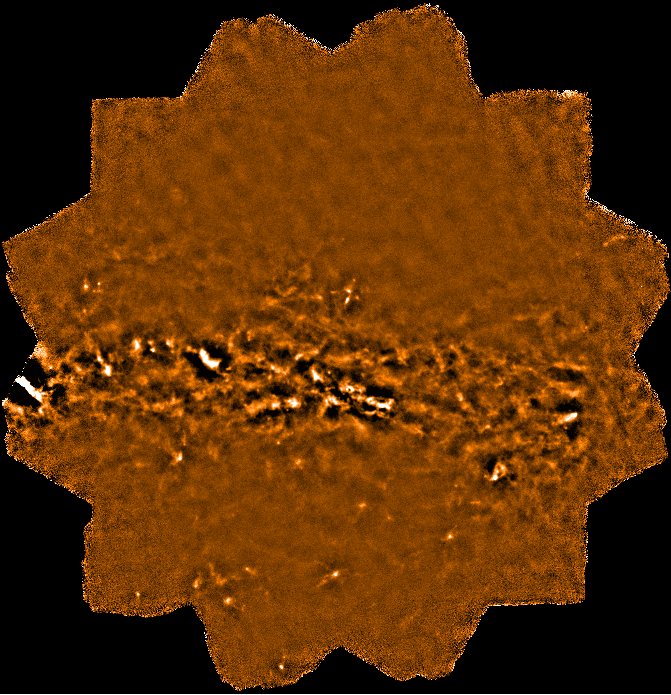
\includegraphics[width=0.47\linewidth]{sc21_gal_def}
\hspace{3mm}
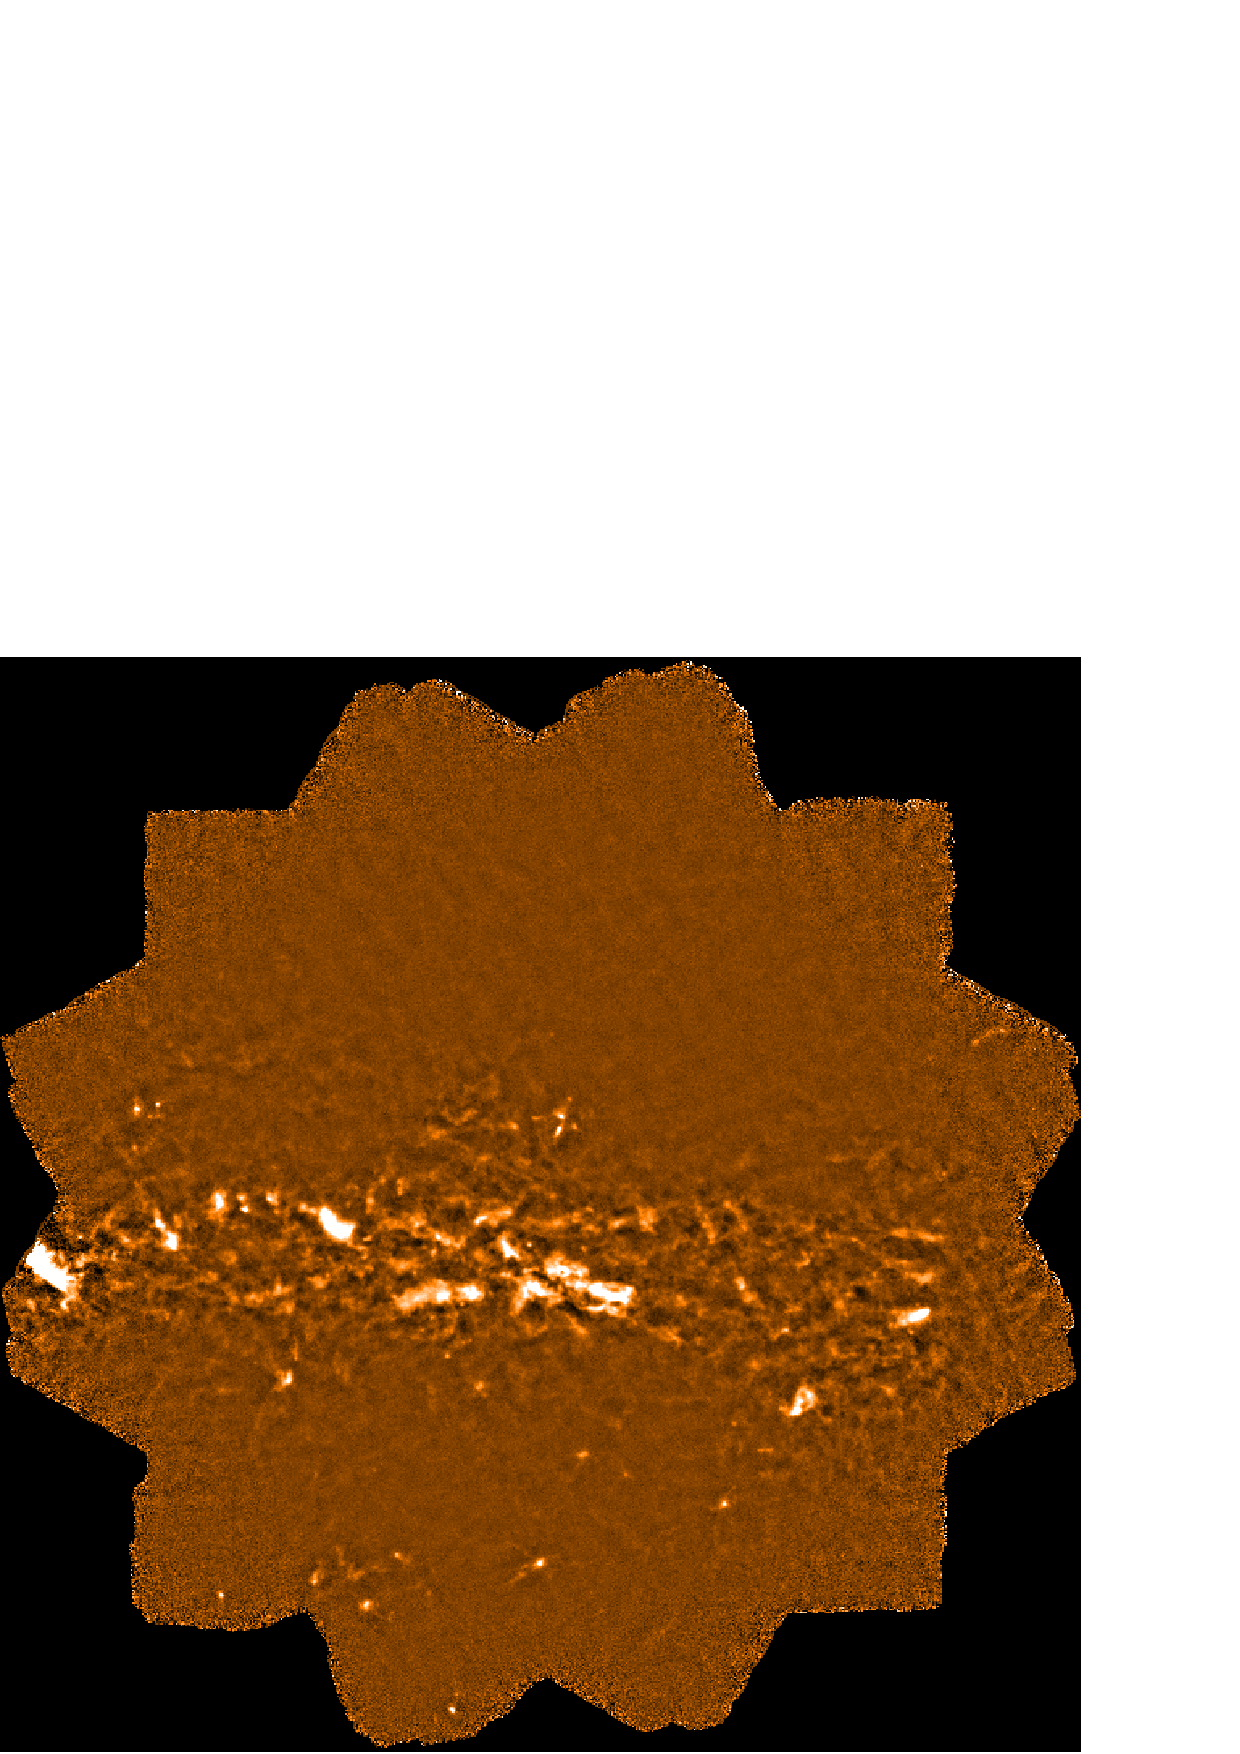
\includegraphics[width=0.47\linewidth]{sc21_gal_brex}
\caption[Example map reduced with
  \file{dimmconfig\_bright\_extended.lis}]
   {A region towards the Galactic Centre reduced with \textbf{(left)}
   default parameter values (\emph{i.e.} no configuration file) \textbf{(right)}
   \file{dimmconfig\_bright\_extended.lis}.\label{fig:becompare}}
\end{figure}

The \brightextended\ configuration is for reducing maps that contain
emission that is extended to some degree and contains some bright
regions. Here \xparam{AST.ZERO_SNR}{ast.zero\_snr} is used to constrain
the \model{AST} model to zero wherever the S/N is lower than 5$\sigma$
(see \cref{Section}{sec:astmask}{AST masking}). \xparam{NUMITER}{numiter}
has been raised to \texttt{-40}, as more iterations are required to
maximise the sensitivity to large dynamic signal ranges in the map.

The other major feature of this configuration is that the subtraction of
the \model{AST} model is skipped on the first five iterations. In
conjunction with the use of \model{FLT} masking, this helps to speed up
convergence and minimise dark bowls around bright source (see
\cref{Section}{sec:skip}{Skipping the AST model}.

\cref{Figure}{fig:becompare}{The images below} shows a comparison
between maps reduced with the default configuration file and using
\file{dimmconfig\_bright\_extended.lis}; the most noticeable
difference is the improvement in the bowling around strong sources.

\latex{\renewcommand*\arraystretch{1}}
\begin{table}[h!]
\centering
\begin{tabular}{|p{6.5cm}p{6.5cm}|}
\hline
\multicolumn{2}{|l|}{\file{dimmconfig\_bright\_extended.lis}}\\
\hline
\setparam{NUMITER}{numiter}{-40}&\setparam{FLT.FILT_EDGE_LARGESCALE}{flt.filt\_edge\_largescale}{480}\\
\setparam{AST.ZERO_SNR}{ast.zero\_snr}{3}&\setparam{AST.ZERO_SNRLO}{ast.zero\_snrlo}{2}\\
\setparam{AST.SKIP}{ast.skip}{5}&\setparam{FLT.ZERO_SNR}{flt.zero\_snr}{5}\\
\setparam{FLT.ZERO_SNRLO}{flt.zero\_snrlo}{3}& \\
\hline
\end{tabular}
\end{table}


\section{\xlabel{problem}Configuration files for solving specific problems}
\label{sec:problem}

Two additional configuration files are available that can be used to supplement your
configuration file in order to solve specific problems:

\begin{itemize}[noitemsep]

\item \fixconvergence\ to help your map converge. It does this by preventing masks
from changing, and by freezing the flags that identify aberrant bolometers. Both of
these restrictions are imposed only after 10 iterations have been performed.

\item \fixblobs\ to remove large ``blooms'' or smooth blobs of spurious emission
in your map. These can be caused by ringing induced by unidentified steps or
spikes in the bolometer time-streams. The fix is to look for oscillations
within the time-streams following the \model{FLT} model, and flag such
time-slices as unusable.  In addition, time slices at which the four sub-arrays
see significantly different common-mode values are also flagged as unusable.

\end{itemize}

These files provide a few additional settings that should be added to
some other configuration in order to achieve the desired fix. For
instance, a configuration file containing the following two lines would
indicate that values from both \file{dimmconfig\_bright\_extended.lis} and
\file{dimmconfig\_fix\_blobs.lis} should be used:

\begin{terminalv}
^/star/share/smurf/dimmconfig_bright_extended.lis
^/star/share/smurf/dimmconfig_fix_blobs.lis
\end{terminalv}

This reads a set of configuration parameter from the
\file{dimmconfig\_bright\_extended.lis} file, and then assigns new values for just
those parameters defined in \file{dimmconfig\_fix\_blobs.lis}. These values override
the values specified in \file{dimmconfig\_bright\_extended.lis}.

The parameters in these files are discussed further
\cref{Chapter}{sec:tweak}{Tailoring Your Reduction}.




\newpage
\chapter{\xlabel{pipeline}The SCUBA-2 Pipeline}
\label{sec:pipe}

\section{\xlabel{pl_overview}Pipeline overview}

SCUBA-2 data-reduction pipelines have been developed based on the
existing \oracdr\ pipeline (Cavanagh et al., 2008\cite{oracdr}) used
for ACSIS. There are three distinct pipelines currently utilised by
SCUBA-2. Users will likely only need to run the science pipeline. The
other two pipelines are designed to run at the JCMT---the quick-look (QL) and
summit pipelines. The latter two are run in real time at the JCMT
during data acquisition.

\begin{itemize}
\item The science pipeline has access to all the data observed for a
given project and adopts a best-possible reduction approach. Images are
made for each complete observation which are combined to create the final
image. Users wishing to reduce their own data should use this pipeline.
This pipeline is responsible for producing the reduced data that is
accessible to users via CADC.
\item The QL runs quality assurance checks on the data as they arrive.
For science data, it calculates the noise between 2\,Hz and 10\,Hz,
along with the NEP and effective NEP, for each 30-second scan. These
values undergo quality-assurance checks to ensure SCUBA-2 is within
an acceptable operating range.
\item The summit pipeline is designed to provide a quick map of the
data, it does this by running fewer iterations and chunking the data
more. This is a useful guide to observers who wish to check the
quality of their data.

\end{itemize}

The manual for the SCUBA-2 pipeline can be found at \pipelinesun,
while the pipeline software comes as part of the \starlink\ suite.
Data-reduction tutorials are available
\href{https://www.eaobservatory.org/jcmt/science/reductionanalysis-tutorials/}{online}\footnote{
\url{https://www.eaobservatory.org/jcmt/science/reductionanalysis-tutorials/}}

\section{\xlabel{science_pl}The science pipeline}

The science pipeline will perform the following:
\vspace{-0.3cm}
\begin{itemize}\itemsep-0.3em
\item Run the iterative map-maker.
\item Apply the FCF to calibrate to mJy/beam or mJy/arcsec$^2$.
\item Co-add multiple observations of the same object.
\item Apply the matched-filter (blank-field configuration file only)
\item Run a source-finding algorithm.
\end{itemize}

\subsection{\xlabel{pl_output}Pipeline recipes}
\label{sec:recipes}

When a project is initially created and MSBs (Minimum Scheduling Blocks)
are constructed using the \href{https://www.eaobservatory.org/jcmt/observing/omp/observing-tool/}{JCMT Observing Tool},
the PI can select a pipeline recipe to assign
to the data. When the data are run through the science pipeline this
recipe is then called by default. This can be overridden on the command
line---see \cref{Section}{sec:parameterfile}{Changing the defaults}.
Described below are the six main \oracdr\ science recipes.

\textbf{Note:} the ``dimmconfig*'' files can be found in:

\begin{terminalv}
% ls $STARLINK_DIR/share/smurf/
\end{terminalv}

\subsection{\xlabel{extsources}\drrecipe{REDUCE\_SCAN}}

\textbf{configuration file: \file{dimmconfig\_jsa\_generic.lis}}

This recipe uses the configuration file \jsageneric\ for \makemap, unless
the sources is identified as a calibrator in which case \file{dimmconfig\_bright\_compact.lis} is used and
FCFs are derived from the map. After all observations have
been processed the data are co-added and calibrated in mJy/beam using
the default FCF. The noise and NEFD properties for the co-add are
calculated and written to log files (\file{log.noise} and
\file{log.nefd} respectively). Finally, the \cupid\ task \findclumps\
is run using the FellWalker algorithm (Berry, 2015\cite{fellwalker}) to
create a source catalogue.

\subsection{\xlabel{extsources}\drrecipe{REDUCE\_SCAN\_CHECKRMS}}

\textbf{Configuration file: \file{dimmconfig\_jsa\_generic.lis}}

This recipe is the same as \drrecipe{REDUCE\_SCAN}, but includes extra
performance estimations determined by \drrecipe{SCUBA2\_CHECK\_RMS}
(see \picard's \xref{\drrecipe{SCUBA2\_CHECK\_RMS}}{sun265}{SCUBA2_CHECK_RMS}). These extra
metrics are written to a log file \file{log.checkrms}. Running
\drrecipe{SCUBA2\_CHECK\_RMS} in the pipeline, rather than as a
standalone \picard\ recipe, allows it to calculate results for
co-added maps.


\subsection{\xlabel{extsources}\drrecipe{REDUCE\_SCAN\_EXTENDED\_SOURCES}}

\textbf{Configuration file: \file{dimmconfig\_bright\_extended.lis}}

This is the recipe for processing extended sources. Multiple
observations are co-added and the output map is calibrated in units of
mJy/arcsec$^2$. This recipe also performs a source-finder routine; the
results are written as a FITS catalogue (with file extension
\file{.FIT}) which can be read as a local catalogue into \gaia.

\subsection{\xlabel{faint}\drrecipe{REDUCE\_SCAN\_FAINT\_POINT\_SOURCES}}

\textbf{Configuration file: \file{dimmconfig\_blank\_field.lis}}

This is the recipe for processing maps containing faint compact
sources. This time the configuration file called by \makemap\ is
\file{dimmconfig\_blank\_field.lis} and the map calibrated in
mJy/beam.  The output map is further processed with a matched filter,
then the S/N is taken to enhance point sources.  A map is written out
at each step.  This recipe also performs a source finder routine; the
results are written as a FITS catalogue (with file extension
\file{.FIT}) which can be read as a local catalogue into \gaia.

\subsection{\xlabel{brightcom}\drrecipe{REDUCE\_SCAN\_ISOLATED\_SOURCE}}

\textbf{Configuration file: \file{dimmconfig\_bright\_compact.lis}}

This is the recipe used for processing calibrator data. It can also
be used for any map of a single bright, isolated source at the
tracking position.

This reduction constrains the map to zero beyond a radius of 1 arc-min
from the source centre. See \cref{Section}{sec:brightcompact}{dimmconfig\_bright\_compact.lis}


\subsection{\xlabel{faintjk}\drrecipe{FAINT\_POINT\_SOURCES\_JACKKNIFE}}

\textbf{Configuration file: \file{dimmconfig\_blank\_field.lis}}

This recipe uses a
\htmladdnormallink{jack-knife}{http://en.wikipedia.org/wiki/Jackknife_resampling}
method to remove residual low-spatial frequency noise and create an
optimal matched-filtered output map. The map-maker is run twice, first
as a standard reduction using \file{dimmconfig\_blank\_field.lis} (and
calibrated in mJy/beam), and the second time with a fake source added
to the time series. This creates a signal map and an effective PSF
map. A jack-knife map is generated from two halves of the dataset and
the maps are `whitened' by the removal of the residual 1/\emph{f}
noise. The whitened signal map is processed with the matched filter
using the whitened PSF map as the PSF input. The data are calibrated
in mJy/beam using a corrected FCF.  See \cref{Section}{sec:jk}{Example
  2 -- Advanced pipeline method} for a more-detailed description of
this recipe and the files produced.


\section{\xlabel{running_pl}Running the science pipeline}
\label{sec:plsteps}

\textbf{Note:} Data-reduction tutorials are available
\href{https://www.eaobservatory.org/jcmt/science/reductionanalysis-tutorials/}{online}.

\begin{aligndesc}
\item[Step~1:]
\textbf{Initialise ORAC-DR}

For 850-micron data, this is done by:
\begin{terminalv}
% oracdr_scuba2_850 -cwd
\end{terminalv}

\vspace{0.2cm}

For 450-micron data, this is done by:

\begin{terminalv}
% oracdr_scuba2_450 -cwd
\end{terminalv}

\vspace{0.2cm}

\item[Step 2:]
\textbf{Set environment variables}

These ensure the data are read from and written to the right
places. Many are set automatically when the pipeline is initialised
but others must be set manually. Details of the optional variables are
given in \pipelinesun\ but the three main ones are:

\begin{itemize}\itemsep-0.1em
\item \envvar{STARLINK\_DIR} -- Location of your Starlink installation.
\item \envvar{ORAC\_DATA\_IN} -- The location where the data should be read from.
If you are supplying a text file listing the raw data this should be the
location of that file.
\item \envvar{ORAC\_DATA\_OUT} -- The location where the data products should be
written. Also used as the location for a user-specified configuration file.
\end{itemize}

Example: Setting \envvar{ORAC\_DATA\_IN} to be the current
directory for C shells (csh, tcsh):

\begin{terminalv}
% setenv ORAC_DATA_IN ./
\end{terminalv}

\newpage

and for Bourne shells (sh, bash, zsh):

\begin{terminalv}
% export ORAC_DATA_IN=./
\end{terminalv}


\item[Step 3:]
\textbf{Run the pipeline}

This is done by:
\begin{terminalv}
% oracdr  -loop file -files <list_of_files>
\end{terminalv}

\vspace{0.2cm}

where the list of files that you wish to reduce can be
an individual or multiple observations (one per line in a text file,
with full path names).

\end{aligndesc}


\begin{tip}
  If you run with -verbose on the command line then you will obtain all messages
 from the Starlink engines (rather than just \oracdr\ messages). This is
 particularly useful for understanding what is occurring during the map-maker stage
 of reduction. This is particularly recommended for new users.
\end{tip}

When executing the \oracdr command, unless ``-nodisplay'' is specified,
a new Xwindow will appear within which
will contain the pipeline output, as shown in \cref{Figures}
{pipeline-oracdr-1}{}--\cref{}{pipeline-oracdr-4}{}.

\begin{figure}
\begin{center}
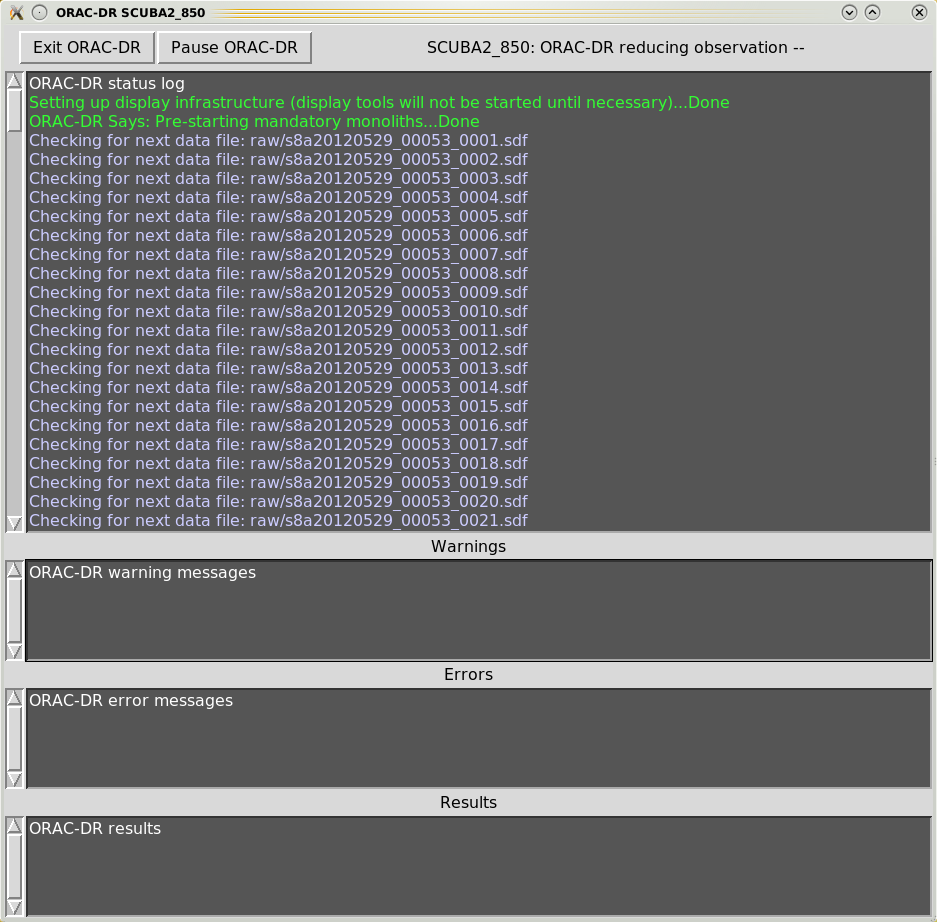
\includegraphics[width=0.7\linewidth]{sc21-pipeline-oracdr-1}
\caption[Output from the pipeline]{The Xwindows output from the \oracdr\
pipeline showing the initial log---here we see the pipeline is checking
for the raw files. \label{pipeline-oracdr-1}}
\end{center}
\end{figure}

\begin{figure}
\begin{center}
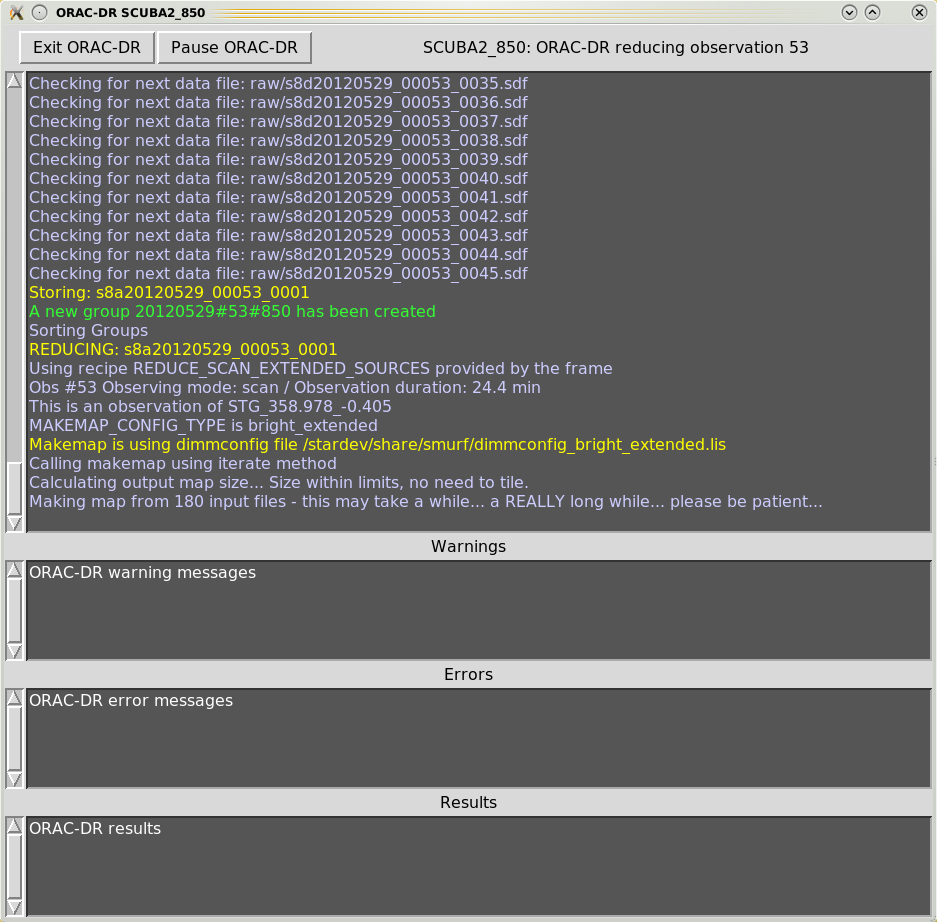
\includegraphics[width=0.7\linewidth]{sc21-pipeline-oracdr-2}
\caption[Output from the pipeline]{The Xwindows output from the \oracdr\
pipeline---here we see the data being reduced with the recipe
REDUCE\_SCAN\_EXTENDED\_SOURCES. The pipeline also reports the name of the
observation being reduced and the duration of the observation. \label{pipeline-oracdr-2}}
\end{center}
\end{figure}

\begin{figure}
\begin{center}
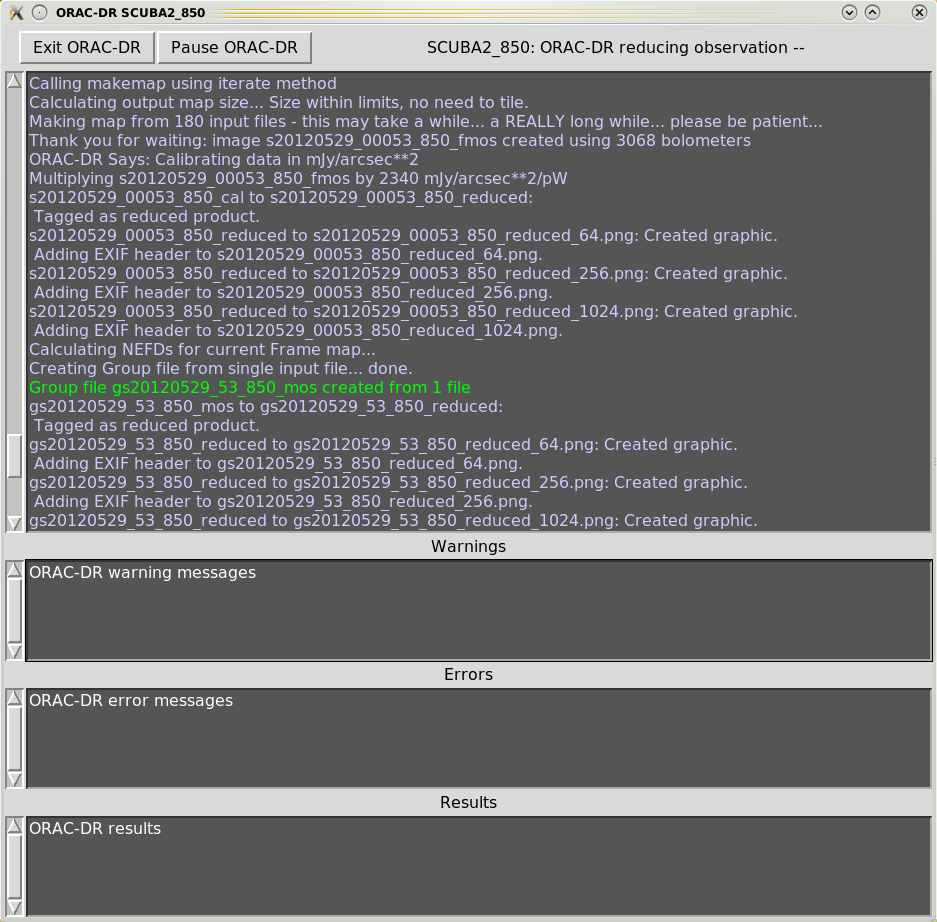
\includegraphics[width=0.7\linewidth]{sc21-pipeline-oracdr-3}
\caption[Output from the pipeline]{The Xwindows output from the \oracdr\
pipeline---here we we see the FCF being applied, the graphics
being created along with a group file (file containing co-added observations
from a single night, if provided). \label{pipeline-oracdr-3}}
\end{center}
\end{figure}


\begin{figure}
\begin{center}
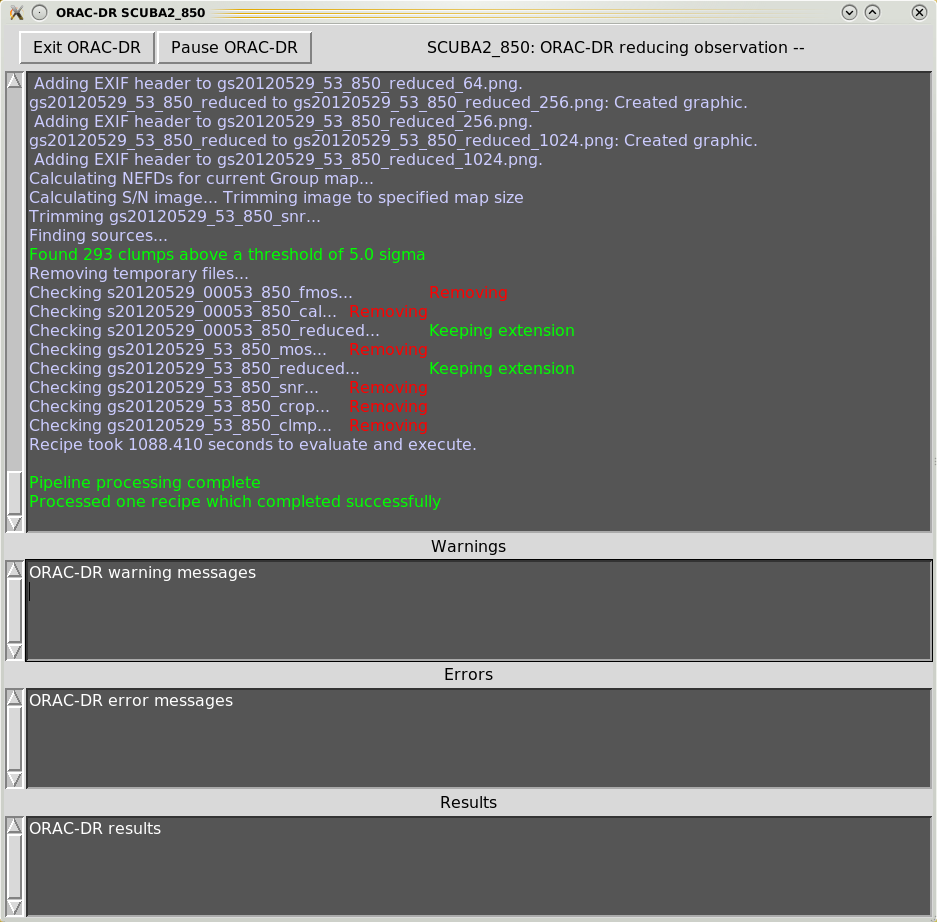
\includegraphics[width=0.7\linewidth]{sc21-pipeline-oracdr-4}
\caption[Output from the pipeline]{The Xwindows output from the \oracdr\
pipeline---here we see the pipeline process has completed. \label{pipeline-oracdr-4}}
\end{center}
\end{figure}




\section{Changing the defaults}
\label{sec:parameterfile}


\subsection{Changing ORAC-DR's behaviour}

{\oracdr}'s behaviour can be changed on the command line. For help simply type


\begin{terminalv}
% oracdr -help
\end{terminalv}

To run the pipeline and obtain all messages from the Starlink engines
(rather than just \oracdr\ messages) you will need to run with verbose (\emph{recommended})

\begin{terminalv}
% oracdr -loop file -files <list_of_files>  -verbose
\end{terminalv}


To run the pipeline and have the results sent to the screen (\param{s)} and to a
file (\param{f}---the file produced is usually called \file{.oracdr\_NNNN.log}
where NNNN is the current process ID. It is written to \$ORAC\_DATA\_OUT
and is a hidden file) is specified using the \param{-log} command.

\begin{terminalv}
% oracdr -files <list_of_files> -loop file  -log sf -verbose
\end{terminalv}



\subsection{Changing the pipeline recipe}
\label{subsec:ChangeRecipe}

You can override the recipe set in the header by listing any different
one on the command line when starting \oracdr. For example
\begin{terminalv}
% oracdr -file <list_of_files> -loop file -log sf REDUCE_SCAN_CHECKRMS
\end{terminalv}

You can find out which recipe is set in the data header via the FITS
header \texttt{RECIPE} keyword in any of your raw files.  For
example both of these options will return the same result (ensure KAPPA
commands are available before running):
\begin{terminalv}
% fitsval s8a20120725_00045_0003 RECIPE
% fitslist s8a20120725_00045_0003 | grep RECIPE
\end{terminalv}

\subsection{Changing the configuration file}

Although each recipe calls one of the standard configuration files
you can specify your own. You will need to create a recipe parameter
file. This file will set the parameter \param{MAKEMAP\_CONFIG} to be
your new configuration file. The first line must be the name of the
recipe used in the reduction.

For example, to run the pipeline with \drrecipe{REDUCE\_SCAN\_CHECKRMS} with a
configuration file called \file{myconfig.lis}, the recipe parameter file
(\file{mypars.ini}) will look like this.
\vspace{0.2cm}
\begin{terminalv}
[REDUCE_SCAN_CHECKRMS]
MAKEMAP_CONFIG = myconfig.lis
\end{terminalv}

Then run the pipeline calling the parameter file via the
\texttt{-recpars} option.
\begin{terminalv}
% oracdr -file <list_of_files> -loop file -log sf -recpars myparams.ini REDUCE_SCAN_CHECKRMS
\end{terminalv}

\subsection{Parameter-file options}

To supply both a new configuration file and a different set of
clump-finding parameters we would update the parameter file
\file{mypars.ini} to look like:

\begin{terminalv}
[REDUCE_SCAN]
MAKEMAP_CONFIG = mynewconfig.lis
FINDCLUMPS_CFG = myfellwalkerparams.lis
\end{terminalv}

Other options we can change in the parameter file include---changing the pixel size

\begin{terminalv}
[REDUCE_SCAN]
MAKEMAP_PIXSIZE = 2
\end{terminalv}

changing output units to mJy/beam

\begin{terminalv}
[REDUCE_SCAN]
CALUNITS = beam
\end{terminalv}

changing output units to mJy/arcsec

\begin{terminalv}
[REDUCE_SCAN]
CALUNITS = arcsec
\end{terminalv}



\section{\xlabel{look_for}What to look out for}
\flushbottom

Once the map-maker has completed you can open your output map using
\gaia\ (see \cref{Figure}{fig:itermap}{this example}). The excerpt in
\cref{Chapter}{sec:manual}{Running \task{makemap} Outside the Pipeline} shows the
output written to the terminal as you run the map-maker. There are a
number of clues in this output that indicate the status of the
reduction.


\begin{figure}
\begin{center}
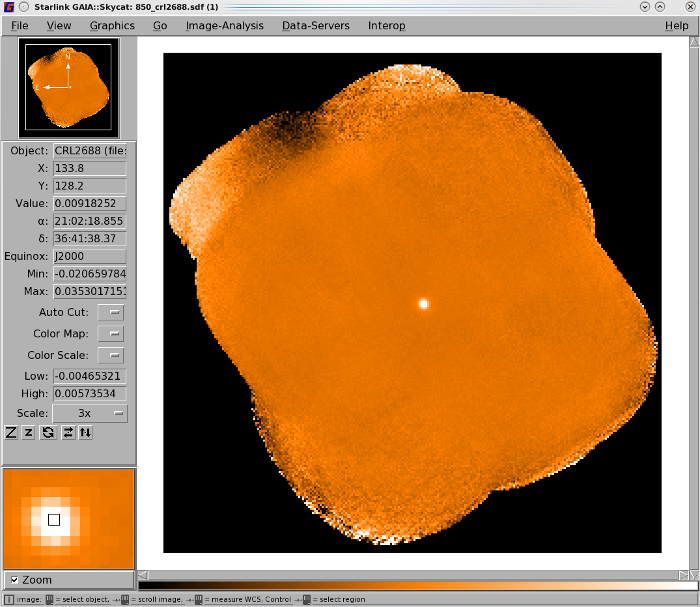
\includegraphics[width=0.7\linewidth]{sc21_crl2688}
\caption[CRL~2688 produced with \makemap]{
  Map of CRL~2688 produced with the \smurf\ task \makemap\ using the
  iterative algorithm with default parameters. \label{fig:itermap}}
\end{center}
\end{figure}

\begin{description}
\item[The number of input files] The first to note is the number of
  input files; it is worth checking this matches your expected
  number. Also summarised are the source name, UT date and scan
  number.

\item[Map dimension] Next the basic dimensions of the data being
  processed are listed near the start of the first iteration. The
  example above has 4\,arcsec pixels---the default at 850$\mu$m.


\item[Chunking] The map-maker then determines if the raw data should
  be split and processed in more than one chunk. In this map the data
  are reduced in one continuous piece: \param{Continuous chunk 1 /
    1}. Chunking is where the map-maker processes sub-sections of the
  time-series data independently and should be avoided if
  possible---see the text box on \latexhtml{Page~\pageref{box:chunk}}{\htmlref{Chunking}{box:chunk}}.
\end{description}


\subsubsection*{Quality statistics}

At the beginning of the reduction, the main purpose of QUALITY
flagging is to indicate how many bolometers are being used. In the
example above you can see that from a total of 5120 bolometers, 1842
were turned off during data acquisition (\texttt{BADDA}). In addition,
136 bolometers exceeded the acceptable noise threshold
(\texttt{NOISE}), while tiny fractions of the data were flagged
because the telescope was moving too slowly (\texttt{STAT}) or the
sample are adjacent to a step that was removed (\texttt{DCJUMP}).

The total number of bad bolometers (\texttt{BADBOL}) is 1984.
Accounting for these, and the small numbers of additionally flagged
samples, 3128.22 effective bolometers are available after initial
cleaning\footnote{The fractional number is due to time-slices being
removed during cleaning. The number of bolometers is then
reconstructed from the number of remaining time-slices.}.


After each subsequent iteration a new `Quality' report is produced,
indicating how the flags have changed. An important flag that appears
in the `Quality' report following the first iteration is \model{COM}:
the DIMM rejects bolometers (or portions of their time series) if they
differ significantly from the common-mode (average) of the remaining
bolometers.

You may note that compared with the initial report, the total number
of samples with good `Quality' (\texttt{Total samples available for
  map}) has dropped from 18634826 to 18273302 (about a 2 per cent
decrease) as additional samples were flagged in each iteration.

Be aware that some large reductions may take many iterations to reach
convergence and you may find significantly fewer bolometers remaining
resulting in higher noise than expected.

\subsubsection*{Convergence}

The convergence criteria \xparam{MAPTOL}{maptol} is updated for each
iteration. The convergence can be checked from the line reporting\\*
\hspace*{0.5cm} \texttt{smf\_iteratemap: *** NORMALIZED MAP CHANGE:
  0.10559 (mean) 2.81081 (max)}

The number to look out for is the mean value of the NORMALIZED MAP CHANGE.
This will have to drop
below your required \param{maptol} for convergence to be achieved.

The default configuration file used in this example executes a maximum
of five iterations, but stops sooner if the change in \param{maptol}
drops below 0.05 (i.e. \param{numiter~=$-$5}). In this example it
stops after five iterations.



\begin{tip}
  You can interrupt the processing at any stage with a single
  \texttt{Ctrl-C}. The map-maker will complete the iteration then
  write out a final science map. Entering \texttt{Ctrl-C} twice will
  kill the process immediately.\widowpenalty=100000
\end{tip}

\section{\xlabel{pl_output}Pipeline output}

The pipeline will produce a \textit{group} file for each object being
processed. If the pipeline is given data from multiple nights, all
those data will be included in the group co-add using inverse variance
weighting.

The final maps in your output directory will have the suffix
\file{\_reduced}. Maps will be made for individual observations, which
will start with an \file{s} for ``SCUBA-2'' (e.g.
\file{s20140620\_00030\_850\_reduced.sdf}). Group maps, which may
contain co-added observations from a single night, are also produced
which have the prefix \file{gs} for ``group SCUBA-2'' and the date/scan
of the \textit{first input file}
(e.g. \file{gs20140620\_30\_850\_reduced.sdf}).

\textbf{Note: A group file is \emph{always} created, even if only a
single observation is being processed.}

Additionally, PNG images are made of the reduced files at a variety of
resolutions.

Another useful feature is that the pipeline will generate log files
to record various useful quantities. The standard log files from
reducing science data are:

\begin{itemize}
\item \file{log.noise}---noise in the map for each observation and the co-add
(calculated from the median of the error array), and
\item \file{log.nefd}---NEFD calculated for each observation and for
the co-added map(s).
\item \file{log.removedobs}---list of observations removed from each
  group (e.g.~due to failing QA).
\end{itemize}

\section{\xlabel{cadc}Getting your data from CADC}

The JCMT Science Archive is hosted by The Canadian Astronomy Data
Centre (CADC). Both raw data and data processed by the science
pipeline are made available to PIs and co-Is through the CADC
interface (\url{http://www3.cadc-ccda.hia-iha.nrc-cnrc.gc.ca/jcmt/}).

To access proprietary data you will need to have your CADC username
registered by the EAO and thereby associated with the project code.
Please contact your friend of project or \url{helpdesk@eaobservatory.org}
to register your account.

An important search option to be aware of is `Group Type', where your
options are Simple, Night, Project and Public. Simple (which becomes
`obs' on the result page) is an individual observation; night means
the group file from the pipeline (these may or may not include more
than one observation; the `Group Members' value will tell you); and
the project option is generated if an entire project has been run
through the pipeline and identical sources across the project are
co-added into master group files.



\newpage
\chapter{\xlabel{manual}Running \task{makemap} Outside the Pipeline}
\label{sec:manual}

The previous chapter described how to make maps using the SCUBA-2 Pipeline.
Users - particularly new users - are encourage to use the pipeline for
their map-making. However, greater control of the map-making
process is available by running the \makemap\ command directly, rather
than from within the pipeline. This chapter describes how to do this, but
should be seen as ``advanced usage''.

\begin{quote}
\emph{
Note, when \makemap\ is run manually (rather than from the pipeline) the
resulting image will be in units of pW, not Jy. Each pixel value
in the map represents the weighted mean value of the bolometer samples
(in pW) that fall within the pixel, after removal of the noise components
described in \cref{Section}{sec:models}{The individual models}. Each
weight is the reciprocal of the variance associated with the bolometer.
Thus each pixel value can be thought of as the astronomical power
received by a typical bolometer at each point on the sky.
\cref{Section}{sec:cmult}{Flux conversion factors} describes how to
convert a map from units of pW to Jy.
}
\end{quote}

\section{Running \texttt{makemap}}

Before running \makemap\ directly, you need to ensure that the Starlink
environment has been initialised and the \smurf\ package started (see
\cref{Section}{sec:starinit}{Initialising Starlink} and
\cref{Section}{sec:packinit}{KAPPA and SMURF for data processing}).

To run \makemap, you  need to supply values for the following
command-line parameters\footnote{Note the distinction between
``command-line parameters'' (also known as ``ADAM'' parameters) that are
supplied on the \texttt{makemap} command line, and ``configuration parameters''
that are specified within a configuration file. Values for all
\emph{configuration} parameters are obtained using a single \emph{command-line}
parameter called \texttt{CONFIG}.}:

\begin{itemize}

\item \texttt{IN} - a list of input NDFs containing raw SCUBA-2 data (see
\cref{Section}{sec:rawdata}{The raw data} and \cref{Section}{sec:ndf}
{Data formats}). There are many ways in which the list of files can be supplied,
as described in Section ``\xref{Specifying Groups of Objects}{sun95}{se_groups}''
in \xref{SUN/95}{sun95}{}. The easiest is to create a simple text
file containing the names of the raw data files -- one per line --- and
then supply the name of the text file, preceded by an up-caret character
(\,\texttt{\^{}}\,), as the value for parameter \texttt{IN}. Note, the names of
the raw data files can contain wild-cards such as ``$*$'' and ``?''.

\item \texttt{OUT} - the name of the NDF in which to store the final
map. The supplied file name should either have a file type of
``\texttt{.sdf}'', or no file type at all (in which case \texttt{.sdf}
will be appended to the supplied value). Any existing file with the same
name will be over-written.

\item \texttt{CONFIG} - a string that specifies new values for one or more
configuration parameters. These new values are used in place of the
\xref{default values}{sun258}{par_full} described in
\xref{SUN/258}{sun258}{}. Any configuration parameter not specified by
the \texttt{CONFIG} string retains its default value. As with files
names, there are many ways in which the group of parameter values can be
specified, and the same documentation should be consulted for details
(\xref{SUN/95}{sun95}{se_groups}). Again, the easiest way is to list the
parameter values in a simple text file with one parameter setting (a
``<name>=<value>'' string) on each line. See \cref{Section}{sec:config}
{Specialised configuration files} for a list of the pre-defined
configuration files that come with \smurf. Note, \texttt{CONFIG}
can be set to the special value ``\texttt{def}'' to force \makemap\ to
use the default values for all parameters. It \emph{is} possible to create
a map using just these default values, but it will not usually be a very
good map. Advice on which parameters to edit can be found in
\cref{Section}{sec:tweak}{Tweaking the configuration file}.

\end{itemize}

If any of the above parameters are \emph{not} given on the \texttt{makemap}
command line, prompts will be issued and the user invited to supply values
for the missing parameters.

So an example command line would be:
\begin{terminalv}
% makemap in=^myfiles.lis out=850_crl2688 \
          config=^$STARLINK_DIR/share/smurf/dimmconfig_bright_compact.lis
\end{terminalv}

Here, the file \texttt{myfiles.lis} contains a list of the raw data
files to be included in the map, and could for instance look like this:

\begin{terminalv}
% cat myfiles.lis
/jcmtdata/raw/scuba2/s8a/20120720/00030/*
/jcmtdata/raw/scuba2/s8b/20120720/00030/*
/jcmtdata/raw/scuba2/s8c/20120720/00030/*
/jcmtdata/raw/scuba2/s8d/20120720/00030/*
\end{terminalv}

This uses all available data for all four 850\,$\mu$m sub-arrays, for
observation 30 taken on 20th July 2012\footnote{The input files should all be
for a single waveband and a single observation --- do not mix files from
different wavebands and/or observations.}.

The file \brightcompact\ is one of the pre-defined configuration files
supplied with \smurf. It contains configuration parameter values that are
optimised for creating maps from bright compact sources.

\begin{tip}
  An up-caret (\,\texttt{\^{}}\,) is required any time you are reading
  in a group text file in \starlink. For the map-maker this includes
  the configuration file (a group of configuration parameters) and the
  list of input files ( a group of NDFs --- \emph{e.g.}  \texttt{in=\^{}\,myfiles.lis}).
\end{tip}

After the \texttt{makemap} command completes, the final map will be left in file
\texttt{850\_crl2688.sdf} and can be displayed using \gaia:

\begin{terminalv}
% gaia 850_crl2688
\end{terminalv}

There are many other command-line parameters that can be supplied when
running \texttt{makemap}, but only the three listed above are mandatory. All the
others assume default values if not supplied on the command-line. For a
full list of all available command-line parameters, their functions and
default values, see the description of \makemap\ within the \textsc{smurf}
document, \xref{SUN/258}{sun258}{}.

You can supply values for any of these extra parameter on the command
line. For instance, one of the command-line parameters that is usually
defaulted is \texttt{PIXSIZE}, which specifies the pixel size for the final
map, in arc-seconds. The default pixel sizes, defined as one quarter of the
Airy disk rounded up to the nearest half arc-second, are:

\begin{itemize}
\item 2\,arcsec at 450$\mu$m
\item 4\,arcsec at 850$\mu$m
\end{itemize}

So for instance, the above command-line could be modified as follows to
produce a map with 3 arc-second pixels:

\begin{terminalv}
% makemap in=^myfiles.lis out=850_crl2688 pixsize=3 \
          config=^$STARLINK_DIR/share/smurf_bright_compact.lis
\end{terminalv}

Note, if parameters are specified by name on the command-line, as
in these examples, then the order in which they are specified is
insignificant\footnote{Some commands, for instance most \textsc{Kappa}
commands, allow the most important parameters to be specified by position
rather than name, in which case their order \emph{is} significant ---
see \xref{\texttt{Specifying Parameter Values on Command Lines}}{sun95}
{se_cmdlindef} in \xref{SUN/95}{sun95}{}.}. Also, parameter names are
case-insensitive.

\begin{tip}
  Map-maker not finding your raw data files from a path? Check you have
  escaped or protected any shell meta-characters in your `in' value,
  for instance by putting double quotes around it or escaping
  wild-cards using a backslash (\emph{e.g.} ``\texttt{in=\textbackslash*.sdf}''
  or just ``\texttt{in=\textbackslash*}''). Note, this issue applies only to
  wild-cards included directly on the command line --- there is no need to
  escape or protect wild cards within a text file.
\end{tip}

\section{Interpreting the screen output from \task{makemap}}

Whilst \makemap\ runs, it outputs information continuously to the screen
about what it is doing. The amount of information displayed can be
controlled using the \xref{\texttt{MSG\_FILTER}}{sun258}{sec_msg} command-line
parameter. It defaults to ``\texttt{normal}'', but if you want more
information you could set it to (say) ``\texttt{verbose}'':

\begin{terminalv}
% makemap in=^myfiles.lis out=850_crl2688 msg_filter=verb \
          config=^$STARLINK_DIR/share/smurf_bright_compact.lis
\end{terminalv}

Note - unambiguous abbreviations may be used for many command line
parameters --- so ``\texttt{verb}'' is acceptable instead of
``\texttt{verbose}''. Setting \texttt{MSG\_FILTER} to ``\texttt{quiet}''
will suppress all screen output.

\begin{tip}
  Map-maker generates a lot of screen output! The main things to check
  are that the ``\texttt{NORMALIZED MAP CHANGE}'' value (the mean value,
  not the max value) decreases nicely towards your requested
  \xparam{MAPTOL}{maptol} value as each iteration is completed, and that
  the ``\texttt{Total samples available for map:}'' value does not fall
  too low (you should usually be looking for values above 50\% of
  maximum). If neither of these two items look problematic, it is usually
  safe to pay less attention to the other screen output.
\end{tip}

The following shows the screen output generated by a typical run of \makemap\
if \texttt{MSG\_FILTER} is left set to its default value of
``\texttt{normal}''. Explanatory comments, which are not actually
part of the output generated by \makemap, are included in \emph{emphasised
type}. The input data is a short observation of a bright compact source
(CRL 2688):

\begin{terminalv}
% makemap in=^myfiles.lis out=850_crl2688 \
          config=^$STARLINK_DIR/share/smurf_bright_compact.lis

Out of 32 input files, 4 were darks, 8 were fast flats and 20 were science
Processing data from instrument 'SCUBA-2' for object 'CRL2688' from the
following observation  :
  20120720 #30 scan
\end{terminalv}

\emph{The output starts by reporting information about the input data files,
including the number that contain on-sky bolometer values (``science''
data), the astronomical object and the SCUBA-2 observation number.}

~
\begin{terminalv}

MAKEMAP: Map-maker will use no more than 92586 MiB of memory

   Projection parameters used:
      CRPIX1 = 0
      CRPIX2 = 0
      CRVAL1 = 315.578333333333 ( RA = 21:02:18.800 )
      CRVAL2 = 36.6938055555556 ( Dec = 36:41:37.70 )
      CDELT1 = -0.00111111111111111 ( -4 arcsec )
      CDELT2 = 0.00111111111111111 ( 4 arcsec )
      CROTA2 = 0

   Output map pixel bounds: ( -132:122, -126:129 )

   Output map WCS bounds:
        Right ascension: 21:01:38.318 -> 21:03:03.280
        Declination: 36:33:07.19 -> 36:50:11.70
\end{terminalv}

\emph{Next comes information about the output map. The world coordinate
system is described by means of the equivalent \htmladdnormallink{FITS-WCS}
{http://fits.gsfc.nasa.gov/fits_wcs.html} keywords\footnote{In fact, NDF
data structures do not use FITS-WCS to describe WCS --- instead they use the
\htmladdnormallink{AST}{http://www.starlink.ac.uk/ast} library, which
provides a much more flexible scheme for handling WCS.}}

\emph{The reported pixel bounds of the output map refer to a pixel coordinate
system in which the source is centred at position (0,0). Note, the definition of
pixel coordinates within the NDF format allows the origin of pixel
coordinates to be at any nominated position within the array --- it does
not have to be at the bottom left corner as in FITS --- and \texttt{makemap}
chooses to put the pixel origin at the specified source position. }

\emph{Finally, the bounds of the map are given in the celestial coordinate
system specified by the \xref{\texttt{SYSTEM}}{sun258}{MAKEMAP} command-line
parameter.  This parameter defaults to ``\texttt{tracking}'', which causes
the map to be created in the celestial coordinate system in which the
observation parameters were originally defined. It may instead be set to a
specific coordinate system (e.g. ``galactic'', ``icrs'', etc.) to force the
map to be made in that system.}

~
\begin{terminalv}
smf_iteratemap: will down-sample data to match angular scale of 4 arcsec
smf_iteratemap: Iterate to convergence (max 40)
smf_iteratemap: stop when mean normalized map change < 0.05
\end{terminalv}

\emph{By default, the data is down-sampled so that the on-sky distance between
adjacent samples is roughly equal to the pixel size (4 arc-seconds in
this case). This saves memory and computing time without adversely
affecting the final map. The degree of down-sampling can be controlled
using the \xparam{DOWNSAMPSCALE}{downsampscale} configuration parameter.}

\emph{Next come information about the stopping criteria for the iterative
map-making algorithm. In this case, iterations will stop when 40 iterations are
completed, or the normalised change in the map between iterations reduces
to less that 0.05. These values are specified by configuration parameters
\xparam{NUMITER}{numiter} and \xparam{MAPTOL}{maptol} (see \cref{Section}
{sec:converge}{Stopping criteria}).}

~
\begin{terminalv}
smf_iteratemap: provided data are in 1 continuous chunks, the largest of which
has 5957 samples (153.729 s)
smf_iteratemap: map-making requires 1626 MiB (map=28 MiB model calc=1598 MiB)
smf_iteratemap: Continuous chunk 1 / 1 =========
\end{terminalv}

\emph{In almost all cases, the raw data files constituting a SCUBA-2
observation will correspond to a single continuous stream of data
samples, taken at roughly 200 Hz. Sometimes however, this may not be the
case\footnote{A common cause of this is if some sub-scans are omitted
from the list of input files supplied to \task{makemap}.}, so the user is
now told how many chunks of data were found, and how long they were.
Something may be wrong if the input data contains any breaks.}

\emph{Next comes information about the amount of memory needed to make
the map. If insufficient memory is available to process all the input
data together, it will be split into chunks, and a separate map made from
each chunk. These maps are later co-added to form the final output map.
This can often result in a poorer map --- see \latexhtml{the box
describing \emph{Data Chunking} on Page~\pageref{box:chunk})~}
{\htmlref{Data Chunking)}{box:chunk}}.}

\emph{Finally, a loop is entered to process each chunk in turn, and the
user is told which chunk is currently being processed. In this
case there  is only one chunk (which is good).}

~
\begin{terminalv}
smf_iteratemap: Iteration 1 / 40 ---------------
\end{terminalv}

We now start the first iteration of the iterative algorithm described in
\cref{Section}{sec:algorithm}{The reduction step-by-step}, to create a
map from the current chunk of  input data. We will be performing ----
at most --- 40 iterations, as set by \xparam{NUMITER}{numiter}.

~
\begin{terminalv}
--- Size of the entire data array ------------------------------------------
bolos  : 5120
tslices: 5957(2.6 min)
Total samples: 30499840
\begin{terminalv}
--- Quality flagging statistics --------------------------------------------
 BADDA:   10805998 (35.43%),        1814 bolos
BADBOL:   10865568 (35.62%),        1824 bolos
DCJUMP:      19631 ( 0.06%),
  STAT:      71680 ( 0.24%),          14 tslices
 NOISE:      41699 ( 0.14%),           7 bolos
Total samples available for map:   19586411, 64.22% of max (3287.97 bolos)
\end{terminalv}

\emph{Now we have a number of statistics describing the cleaned data
prior to the first iteration\footnote{Setting
\texttt{MSG\_FILTER=verbose} on the \texttt{makemap} command line will
generate more information about the cleaning process.}.}

\emph{Each sub-array contains a grid of $32\times40$ bolometers, making 5120
bolometers in total over all four sub-arrays. The number of time slices in
the concatenated data after down-sampling is reported. In this case, 5957
time slices over 2.6 minutes, equating to a down-sampled frequency of about
38 Hz. The total number of samples is the product of the number of
bolometers and the number of time slices. Each of the following lines
indicates the percentage of the data that has been flagged as unusable for
various reasons:}

\begin{itemize}
\item \emph{BADDA - flagged as unusable during data acquisition.}
\item \emph{DCJUMP - flagged as unusable because of a sudden step change in
the base-line.}
\item \emph{STAT - flagged as unusable because the telescope was stationary
(or at least moving too slowly).}
\item \emph{NOISE - flagged as unusable because they were too noisy.}
\end{itemize}

\emph{The BADBOL item gives the fraction of bolometers that have been
flagged as entirely bad for any of these reasons, and from which no data
will be used.}

~
\begin{terminalv}
smf_iteratemap: Calculate time-stream model components
smf_iteratemap: Rebin residual to estimate MAP
smf_iteratemap: Calculate ast
\end{terminalv}

\emph{Indicates the models that are being calculated. More information
about each individual model is displayed if you set
\texttt{MSG\_FILTER=verbose} on the \texttt{makemap} command line.}

~
\begin{terminalv}
--- Quality flagging statistics --------------------------------------------
 BADDA:   10805998 (35.43%),        1814 bolos  ,change          0 (+0.00%)
BADBOL:   11008536 (36.09%),        1848 bolos  ,change     142968 (+1.32%)
DCJUMP:      19631 ( 0.06%),                    ,change          0 (+0.00%)
  STAT:      71680 ( 0.24%),          14 tslices,change          0 (+0.00%)
   COM:     372786 ( 1.22%),                    ,change     372786 (+0.00%)
 NOISE:      41699 ( 0.14%),           7 bolos  ,change          0 (+0.00%)
Total samples available for map:   19214687, 63.00% of max (3225.56 bolos)
     Change from last report:    -371724, -1.90% of previous
smf_iteratemap: Will calculate chi^2 next iteration
smf_iteratemap: *** NORMALIZED MAP CHANGE: 2.22778 (mean) 60.5292 (max)
\end{terminalv}

\emph{More statistics are displayed once the first iteration is completed
and the first estimate of the science map has been generated. Data
samples may be flagged as bad within the iterative stage for various
reasons, and so these statistics may be different to those shown prior to
the start of the iterative stage. Most significantly, the \texttt{COM:}
line shows the percentage of data that has been rejected because the time
stream did not resemble the common-mode signal closely enough. The
``\texttt{NORMALIZED MAP CHANGE}'' values are of no real significance on the
first iteration since there is no previous map with which to compare the
new map (in fact the numerical values are generated by comparing the new map
with a map full of zeros).}

~
\begin{terminalv}
smf_iteratemap: Iteration 2 / 40 ---------------
smf_iteratemap: Calculate time-stream model components
smf_calcmodel_noi: Calculating a NOI variance for each box of 581 samples
using variance of neighbouring residuals.
smf_iteratemap: Rebin residual to estimate MAP
smf_iteratemap: Calculate ast
--- Quality flagging statistics --------------------------------------------
 BADDA:   10805998 (35.43%),        1814 bolos  ,change          0 (+0.00%)
BADBOL:   11038321 (36.19%),        1853 bolos  ,change      29785 (+0.27%)
 SPIKE:         36 ( 0.00%),                    ,change         36 (+0.00%)
DCJUMP:      19631 ( 0.06%),                    ,change          0 (+0.00%)
  STAT:      71680 ( 0.24%),          14 tslices,change          0 (+0.00%)
   COM:     393125 ( 1.29%),                    ,change      20339 (+5.46%)
 NOISE:      41699 ( 0.14%),           7 bolos  ,change          0 (+0.00%)
Total samples available for map:   19194401, 62.93% of max (3222.16 bolos)
     Change from last report:     -20286, -0.11% of previous
smf_iteratemap: *** CHISQUARED = 0.997314089857974
smf_iteratemap: *** NORMALIZED MAP CHANGE: 1.78691 (mean) 8.09056 (max)

\end{terminalv}

\emph{The second iteration starts, and proceeds in much the same way as the
first iteration. The main difference is that the NOI model is generated
at the start of the second iteration. This model measures the variance
within each bolometer time-stream. It is used to weight the bolometer
samples when forming the mean sample value in each map
pixel\footnote{Bolometers are given equal weight in the map created at
the end of the first iteration since the NOI model has not yet been
calculated at that point.}. NOI is calculated from the residuals left after
removal of all other models, and is only calculated once --- subsequent
iterations re-use the same NOI values.}

\emph{The \texttt{SPIKE:} item that has appeared in the quality flagging
statistics records the number of samples that have been rejected as
transient spikes in the time-series. This flagging is done by comparing
the bolometer values that fall in each map pixel, and flagging any that
appear to be statistical out-liers - see configuration parameter
\xparam{AST.MAPSPIKE}{ast.mapspike}.}

\emph{The mean ``\texttt{NORMALIZED MAP CHANGE}'' value should drop with each
subsequent iteration (note, the ``max'' normalised map change value
can usually be ignored as it records the maximum normalised change in any
single map pixel and is thus highly subject to random variations).}

~
\begin{terminalv}
smf_iteratemap: Iteration 3 / 40 ---------------
smf_iteratemap: Calculate time-stream model components
smf_iteratemap: Rebin residual to estimate MAP
smf_iteratemap: Calculate ast
--- Quality flagging statistics --------------------------------------------
 BADDA:   10805998 (35.43%),        1814 bolos  ,change          0 (+0.00%)
BADBOL:   11050235 (36.23%),        1855 bolos  ,change      11914 (+0.11%)
 SPIKE:         36 ( 0.00%),                    ,change          0 (+0.00%)
DCJUMP:      19631 ( 0.06%),                    ,change          0 (+0.00%)
  STAT:      71680 ( 0.24%),          14 tslices,change          0 (+0.00%)
   COM:     401600 ( 1.32%),                    ,change       8475 (+2.16%)
 NOISE:      41699 ( 0.14%),           7 bolos  ,change          0 (+0.00%)
Total samples available for map:   19185947, 62.91% of max (3220.74 bolos)
     Change from last report:      -8454, -0.04% of previous
smf_iteratemap: *** CHISQUARED = 0.976599086972009
smf_iteratemap: *** change: -0.0207150028859653
smf_iteratemap: *** NORMALIZED MAP CHANGE: 0.305 (mean) 1.24407 (max)
\end{terminalv}

\emph{The mean normalised map change continues to drop with the third
iteration, as expected. The total number of samples going into the map is
dropping with each iteration, but only very slowly. This is mainly due to
the increased number of samples being flagged by the COM model, but is at
an acceptably small level.}

~
\begin{terminalv}
smf_iteratemap: Iteration 4 / 40 ---------------
smf_iteratemap: Calculate time-stream model components
smf_iteratemap: Rebin residual to estimate MAP
smf_iteratemap: Calculate ast
--- Quality flagging statistics --------------------------------------------
 BADDA:   10805998 (35.43%),        1814 bolos  ,change          0 (+0.00%)
BADBOL:   11056192 (36.25%),        1856 bolos  ,change       5957 (+0.05%)
 SPIKE:         36 ( 0.00%),                    ,change          0 (+0.00%)
DCJUMP:      19631 ( 0.06%),                    ,change          0 (+0.00%)
  STAT:      71680 ( 0.24%),          14 tslices,change          0 (+0.00%)
   COM:     409883 ( 1.34%),                    ,change       8283 (+2.06%)
 NOISE:      41699 ( 0.14%),           7 bolos  ,change          0 (+0.00%)
Total samples available for map:   19177684, 62.88% of max (3219.35 bolos)
     Change from last report:      -8263, -0.04% of previous
smf_iteratemap: *** CHISQUARED = 0.96404406922676
smf_iteratemap: *** change: -0.0125550177452489
smf_iteratemap: *** NORMALIZED MAP CHANGE: 0.0401588 (mean) 0.151877 (max)
\end{terminalv}

\emph{After the fourth iteration the mean normalised map change has
dropped to 0.0401588, which is below the value of 0.05 provided for the
\xparam{MAPTOL}{maptol} parameter by the \brightcompact\
configuration file\footnote{In fact, 0.05 is the default \texttt{maptol}
value, which is left unchanged by \texttt{dimmconfig\_bright\_compact.lis}.}.
Consequently, \texttt{makemap} considers the map to have converged. However,
in view of the fact that the \brightcompact\ configuration file uses
``AST masking'' (see \cref{Section}{sec:astmask}{AST masking}), it is
necessary to do one final iteration in order to assign correct values to
the pixels that lie outside the source mask. Note, when AST masking is being
used, the reported normalised map change values only include pixels that
are within the source mask.}

~
\begin{terminalv}
smf_iteratemap: Iteration 5 / 40 ---------------
smf_iteratemap: Calculate time-stream model components
smf_iteratemap: Rebin residual to estimate MAP
smf_iteratemap: Calculate ast
--- Quality flagging statistics --------------------------------------------
 BADDA:   10805998 (35.43%),        1814 bolos  ,change          0 (+0.00%)
BADBOL:   11068106 (36.29%),        1858 bolos  ,change      11914 (+0.11%)
 SPIKE:         36 ( 0.00%),                    ,change          0 (+0.00%)
DCJUMP:      19631 ( 0.06%),                    ,change          0 (+0.00%)
  STAT:      71680 ( 0.24%),          14 tslices,change          0 (+0.00%)
   COM:     414727 ( 1.36%),                    ,change       4844 (+1.18%)
 NOISE:      41699 ( 0.14%),           7 bolos  ,change          0 (+0.00%)
Total samples available for map:   19172853, 62.86% of max (3218.54 bolos)
     Change from last report:      -4831, -0.03% of previous
smf_iteratemap: *** CHISQUARED = 0.964032127175568
smf_iteratemap: *** change: -1.19420511923707e-05
smf_iteratemap: *** NORMALIZED MAP CHANGE: 0.0157131 (mean) 0.103135 (max)
smf_iteratemap: ****** Completed in 5 iterations
smf_iteratemap: ****** Solution CONVERGED
Setting 24282 map pixels bad because they contain fewer than 4 samples (=0.01
of the mean samples per pixel).
Total samples available from all chunks: 19172853 (3218.54 bolos)
\end{terminalv}

\emph{After the extra iteration required by AST masking has been
performed, the final output map is created. It is always advisable to
check the final number of samples available for the map, as a low value
will cause your map to have high noise levels. In this case, 62.86\% of
the samples are available for the map, which is quite acceptable --- only
a couple of percent of the samples have been rejected by the map-making,
mostly flagged by the COM model. The bulk of the bad samples (35.43\%)
were rejected during data acquisition due to dead bolometers \emph{etc}.}

\emph{Note, the \xparam{NUMITER}{numiter} parameter is set to -40 by
\brightcompact, meaning that no more than 40 iterations will be
performed. In this particular case we only needed 4 iteration (plus a
mandatory extra iteration) to achieve
our requested \xparam{MAPTOL}{maptol} value. But it is possible for some
observations --- particularly observations of extended sources --- to
require more than 40 iterations to converge to a \texttt{maptol} of 0.05.
In such cases the screen output will end with a message saying that the
solution ``FAILED TO CONVERGE''\footnote{However a map will still be
created, but should be used with caution.}. In such cases, you \emph{could}
simply increase \texttt{numiter} and re-run \texttt{makemap}, but you may
also want to investigate the cause of the slow convergence using one or more
of the techniques described in \cref{Chapter}{sec:raw}{Chapter 9}, as it
may indicate some issue with the raw data.}

\emph{Map pixels that receive a very small number of samples are automatically
set bad. These are usually the pixels around the periphery of the
observation, and will have very unreliable variance estimates. The
threshold is determined by the \xparam{HITSLIMIT}{hitslimit} parameter,
which defaults to 1 percent of the mean number of hits per pixel,
corresponding to 4 samples per pixel in this case.}

\emph{The observation used in this particular case was a short
observation of a calibrator, lasting only 2.6 minutes. Consequently there
was no need to divide the data up into multiple chunks in order to fit it
into memory.  However, for very long observations, or for shorter
observations when using a computer with less than the recommended amount
of memory (see \cref{Section}{sec:computing}{Chapter 1}), it may be
necessary to process the raw data in multiple chunks. If this happens, a
map is created from each chunk in turn, and all these maps are then added
together to form the final map.  The final message ``\texttt{Total
samples available from all chunks: 19172853 (3218.54 bolos)}'' indicates
the total number of samples (and equivalent number of bolometers) used
from all chunks. In this case there was only one chunk, so these values
are equal to the numbers reported at the end of the last iteration.}

\section{Interacting with \texttt{makemap} during a long run}
For long observations, \makemap\ can take several hour to run,
particularly on slow or low memory computers. For this reason it is
useful to be able to monitor progress so that potential problems can be
detected early, in order to avoid wasting time.

\subsection{Monitoring screen output}
The most straight-forward way of monitoring progress is to check the
values written to the screen by \texttt{makemap} at the end of each iteration (see
the previous section). For instance, if you run \texttt{makemap} as follows:

\begin{terminalv}
% makemap in=^infiles out=outmap config=^conf | tee makemap.log
\end{terminalv}

then the messages displayed by makemap on the screen will also be written
to text file \texttt{makemap.log}. This makes it easy to search the log
file whilst \texttt{makemap} is still running, for instance from another terminal
window:

\begin{terminalv}
% grep NORMALIZED makemap.log
smf_iteratemap: *** NORMALIZED MAP CHANGE: 1.02829 (mean) 20.7922 (max)
smf_iteratemap: *** NORMALIZED MAP CHANGE: 0.739832 (mean) 9.81836 (max)
smf_iteratemap: *** NORMALIZED MAP CHANGE: 0.370128 (mean) 5.42933 (max)
smf_iteratemap: *** NORMALIZED MAP CHANGE: 0.258304 (mean) 3.2717 (max)
smf_iteratemap: *** NORMALIZED MAP CHANGE: 0.205415 (mean) 2.66815 (max)
smf_iteratemap: *** NORMALIZED MAP CHANGE: 0.177044 (mean) 2.28417 (max)
smf_iteratemap: *** NORMALIZED MAP CHANGE: 0.159569 (mean) 2.05803 (max)
\end{terminalv}

This displays the normalised change in maps between successive
iterations, for the iterations that have so far been completed. If the mean
normalised map change is not decreasing smoothly,
(for instance if it is oscillating around a fixed value), then there is a
potential problem. In which case you may want to interrupt the
\texttt{makemap} process, rather than waiting potentially for several
hours just to end up with a bad map.

Likewise, it is useful to monitor the total number of samples that are
being pasted into the map at the end of each iteration:

\begin{terminalv}
% grep "Total samples" makemap.log
Total samples: 299919360
Total samples available for map:  174105275, 58.05% of max (2972.2 bolos)
Total samples available for map:  171284110, 57.11% of max (2924.03 bolos)
Total samples available for map:  171242020, 57.10% of max (2923.32 bolos)
Total samples available for map:  171239147, 57.10% of max (2923.27 bolos)
\end{terminalv}

The lower the percentage of samples included in the map, the greater will
be the noise in the map. If this number drops much below 50\% then you
may want to think about aborting \texttt{makemap} and investigating why
the number is so low (\emph{e.g.} by looking at the ``quality
statistics'' displayed at the end of each iteration, to determine the
cause of the data loss).

Likewise, information can be gather about chunking:

\begin{terminalv}
% grep chunk makemap.log
smf_iteratemap: provided data are in 7 continuous chunks, the largest of
which has 487 samples (10.1534 s)
smf_iteratemap: Continuous chunk 1 / 7 =========
smf_iteratemap: Adding map estimated from this continuous chunk to total
smf_iteratemap: Continuous chunk 2 / 7 =========
smf_iteratemap: Adding map estimated from this continuous chunk to total
smf_iteratemap: Continuous chunk 3 / 7 =========
smf_iteratemap: Adding map estimated from this continuous chunk to total
\end{terminalv}

This indicates that the raw data has gaps in it, resulting in seven maps
being made, one from each continuous chunk, before the final map is made
by combining all the individual maps. Chunking can produce sub-optimal
maps, and should normally be investigated - see \latexhtml{the description
of \emph{Data Chunking} on Page~\pageref{box:chunk})~}{\htmlref{Data
Chunking}{box:chunk}}.

\subsection{Monitoring the map at the end of each iteration}
\label{sec:itermaps}
The map created at the end of each iteration is normally discarded, but can
be saved by setting configuration parameter \xparam{ITERMAP}{itermap}
to either 1 or 2. By default, these ``itermaps'' are written to an
extension of the main output NDF as described in
\cref{Section}{sec:inter}{Writing out models and intermediate maps}, and
cannot be viewed until \makemap\ has completed. However, an alternative
destination for these itermaps can be specified on the \texttt{makemap}
command-line as follows, allowing them to be viewed whilst \texttt{makemap}
is still running:

\begin{terminalv}
% cat conf
^STARLINK_DIR/share/smurf/dimmconfig_jsa_generic.lis
itermap=1
%
% makemap in=^infiles out=outmap config=^conf itermaps=myitermaps
\end{terminalv}

Note the distinction between the ``\texttt{itermaps}'' (plural)
\emph{command-line} option, and the ``\texttt{itermap}'' (singular)
\emph{configuration} parameter.  As soon as the first iteration has
finished, the above command will create a new file
called \texttt{myitermaps.sdf} in which each itermap will be stored as soon
as it is created. The file is closed after each itermap is written, and
re-opened again before writing the next itermap. This is an example of a
\emph{container file}, where a single \texttt{.sdf} file contains several
NDFs, each holding a different map (see \cref{Section}{sec:ndf}{Data
formats}). You can list the maps in such a file using \textsc{Kappa}
\xref{\task{ndfecho}}{sun95}{NDFECHO} as follows:

\begin{terminalv}
% ndfecho myitermaps
myitermaps.CH00I001
myitermaps.CH00I002
myitermaps.CH00I003
myitermaps.CH00I004
myitermaps.CH00I005
myitermaps.CH00I006
myitermaps.CH00I007
...
\end{terminalv}

The name of each itermap is of the form ``CHxxIyyy'', where ``xx'' is the
chunk number and ``yyy'' is the iteration number. In the common case
where all raw data is processed in a single chunk, ``xx'' will be ``00''
for all itermaps.

You can view a single itermap using:
\begin{terminalv}
% gaia myitermaps.CH00I004
\end{terminalv}

If you want to view several itermaps side-by-side, you can use \textsc{Kappa}
\xref{\task{picgrid}}{sun95}{PICGRID} to divide the screen up into a grid
of ``pictures'', then use \xref{\task{picsel}}{sun95}{PICSEL} to pick each
picture in turn, and use \xref{\task{display}}{sun95}{DISPLAY} to display
an itermap in each one. For instance to display the first six itermaps
side-by-side in a $3 \times 2$ grid, all with the same scaling, without
any axes, do:

\begin{terminalv}
% gdclear
% picgrid 3 2
% picsel 1
% display myitermaps.CH00I001 axes=no mode=percentiles percentiles=\[2,98\]
% picsel 2
% display myitermaps.CH00I002 mode=current
% picsel 3
% display myitermaps.CH00I003 mode=current
% picsel 4
% display myitermaps.CH00I004 mode=current
% picsel 5
% display myitermaps.CH00I005 mode=current
% picsel 6
% display myitermaps.CH00I006 mode=current
\end{terminalv}

This produces the display shown in \cref{Figure}{fig:itermaps}{Initial
six itermaps}. \textsc{Kappa} \xref{\task{display}}{sun95}{DISPLAY} has
many options for controlling things like data scaling, axis annotation
and style, colour table, graphics device, \emph{etc.}.

\begin{figure}
\begin{center}
  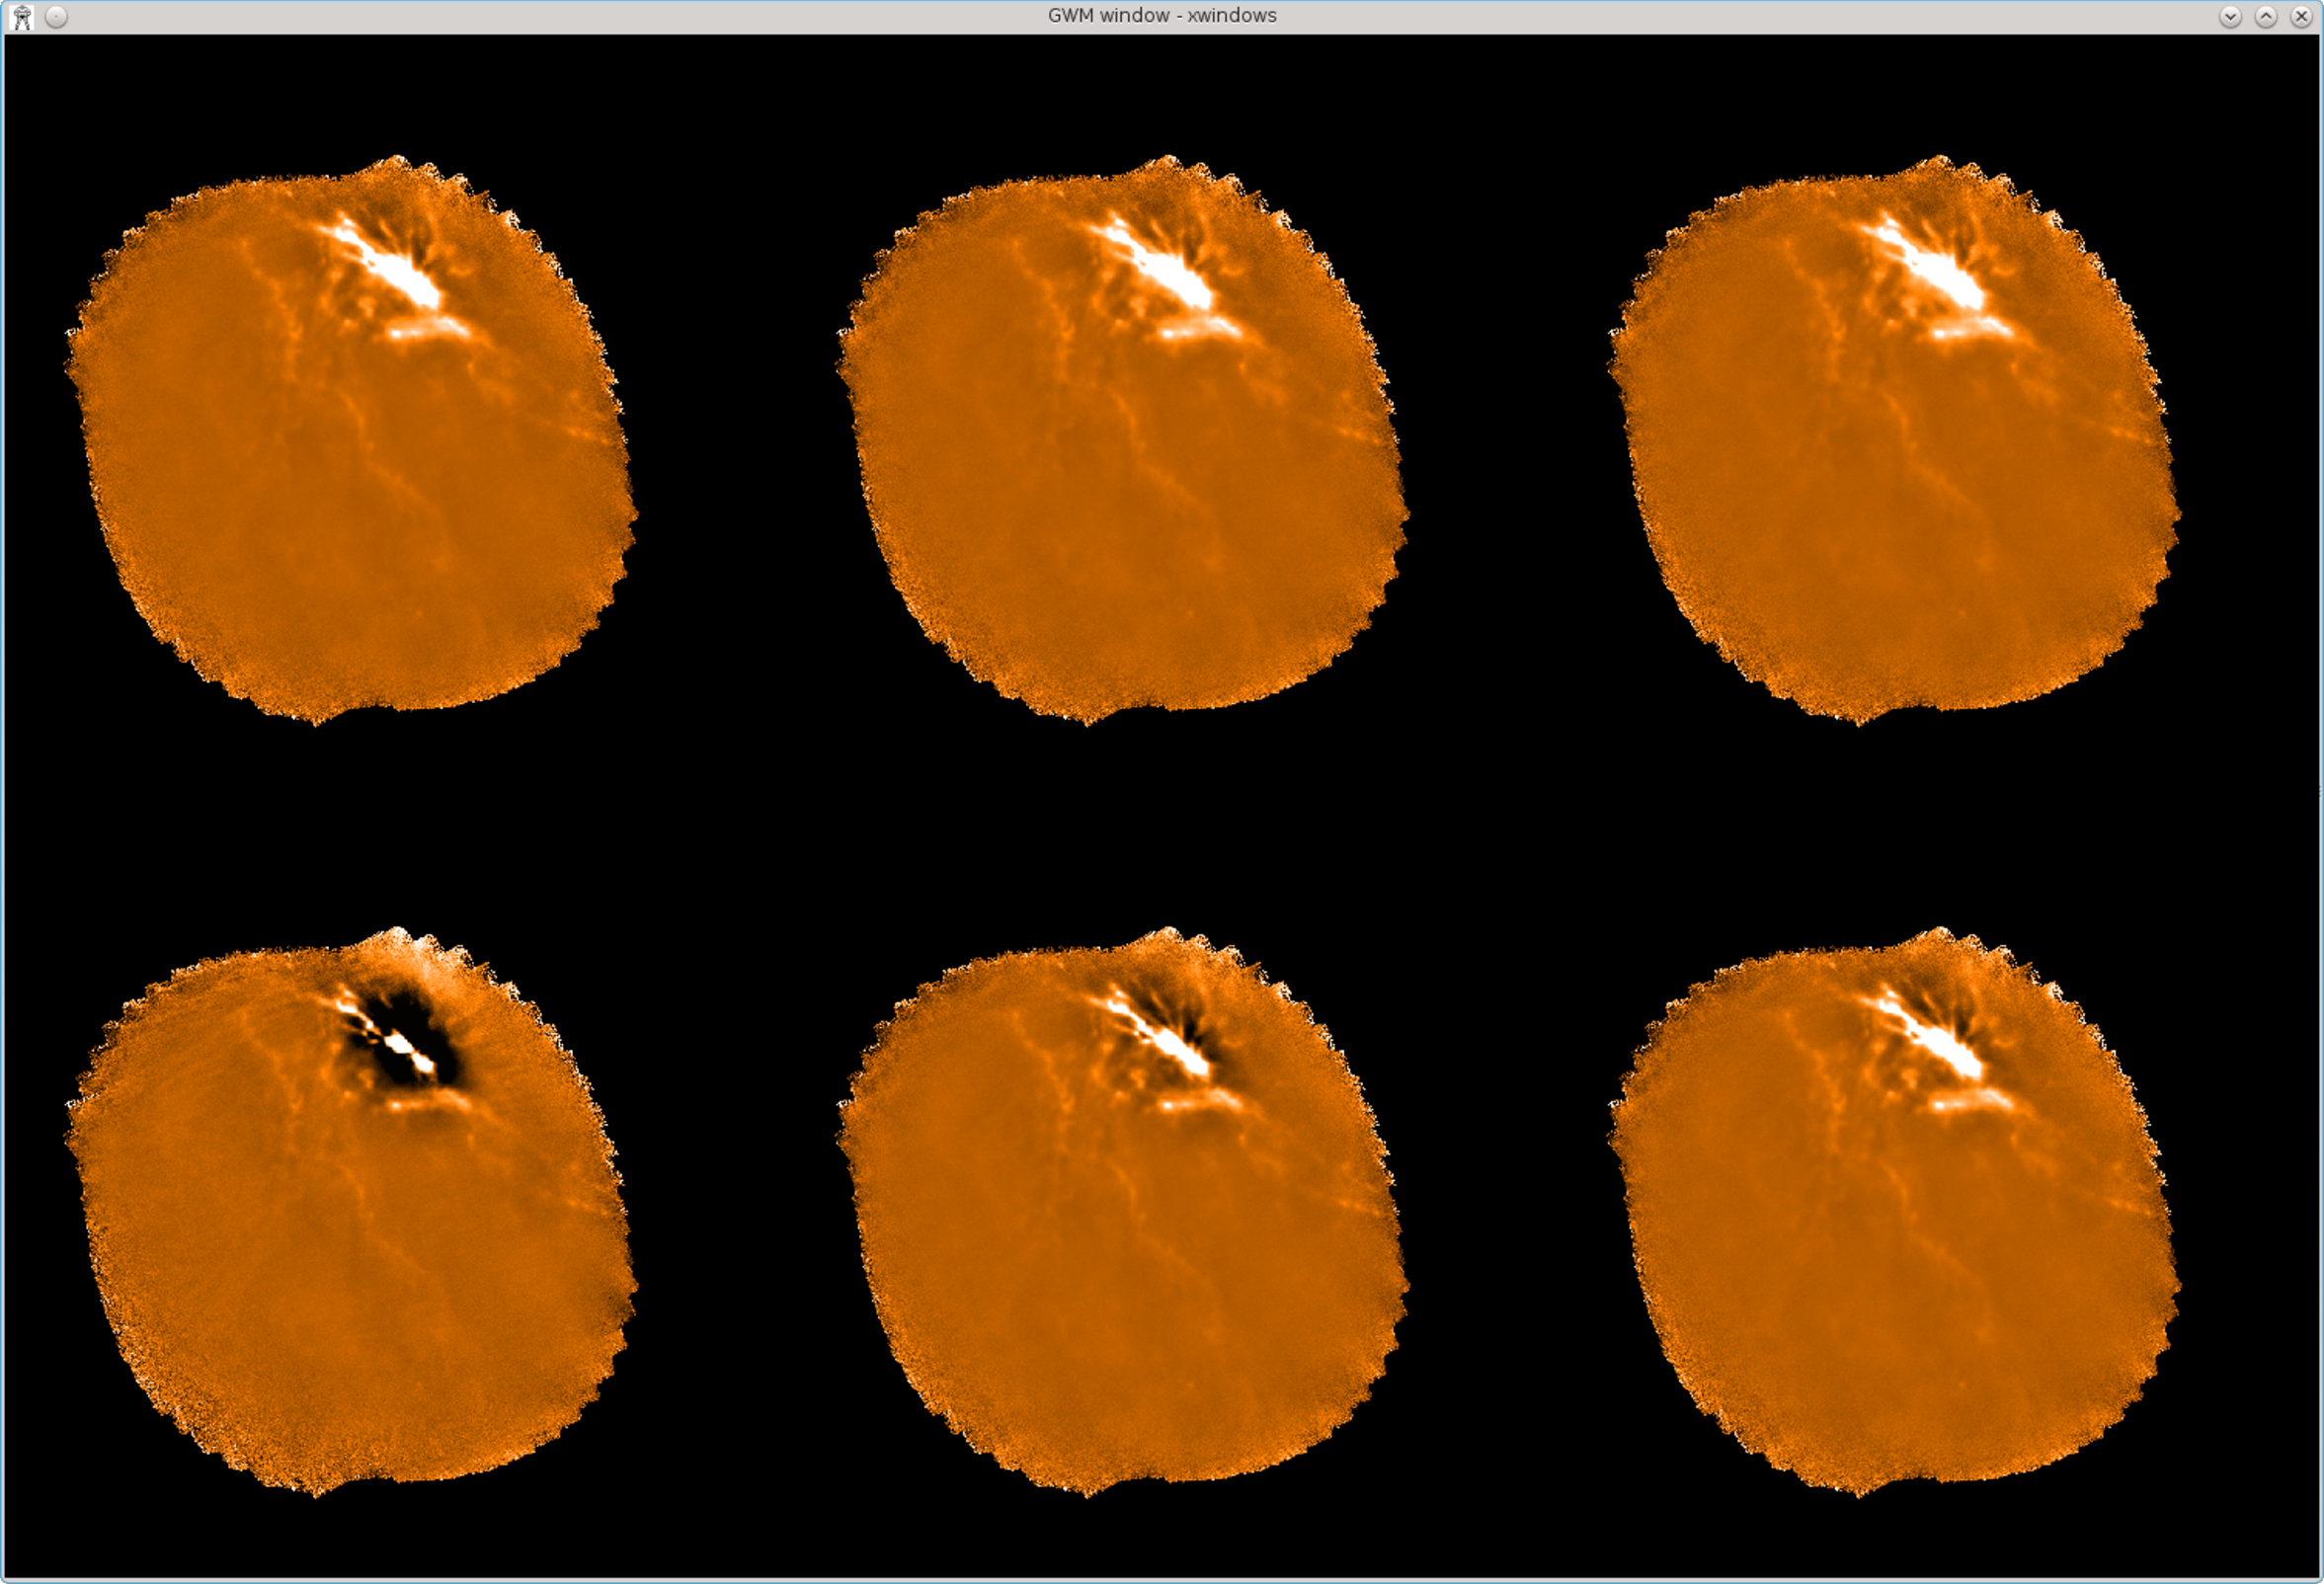
\includegraphics[width=\linewidth]{sc21_itermaps}
\end{center}
\caption[Initial six itermaps]{\small The maps created on the first six
iterations of \texttt{makemap}, from an observation of Orion A, using the
\texttt{dimmconfig\_jsa\_generic.lis} configuration file with the addition
of ``\texttt{itermap=1}''. The first map is bottom left, and the sixth
map is top right. This illustrates the initial fast improvement
in the map over the first few iterations.}
\label{fig:itermaps}
\end{figure}

Alternatively, you can combine the itermaps into a 3D cube, and then use
the cube-viewing facilities of \gaia\ to scroll through the itermaps in the
style of a movie (see \cref{Section}{sec:inter}{Writing out models and
intermediate maps})\footnote{Note, \textsc{smurf} \stackframes\ can be used
instead of \textsc{Kappa} \xref{\task{paste}}{sun95}{PASTE} if preferred.}:

\begin{terminalv}
% paste in=myitermaps out=itercube shift=\[0,0,1\]
% gaia itercube
\end{terminalv}

It is sometimes informative
to look at the \emph{change} between
itermaps, to see the incremental effect of each iteration. This is most
easily done if the itermaps are first stacked into a cube as described
above. The next step is to produce a copy of the cube in which the pixel
origin is moved by one pixel along the third axis (\emph{i.e.} the axis
that enumerates iteration). Finally subtract one cube from the other, and
display the resulting difference cube (this example shows how command-line
parameters can often be specified by position instead of by name when
running \textsc{Kappa} commands --- check the help information for each
command to see the order in which options should be supplied):

\begin{terminalv}
% paste myitermaps out=itercube shift=\[0,0,1\]
% slide itercube itercube-shifted \[0,0,1\] near
% sub itercube-shifted itercube diffcube
%
% picsel 1
% display diffcube'(,,1)' axes=no mode=percentiles percentiles=\[2,98\]
% picsel 2
% display diffcube'(,,2)' mode=current
% picsel 3
% display diffcube'(,,3)' mode=current
% picsel 4
% display diffcube'(,,4)' mode=current
% picsel 5
% display diffcube'(,,5)' mode=current
% picsel 6
% display diffcube'(,,6)' mode=current
\end{terminalv}

This produces the display shown in \cref{Figure}{fig:diffmaps}{Initial
six difference maps}.

\begin{figure}
\begin{center}
  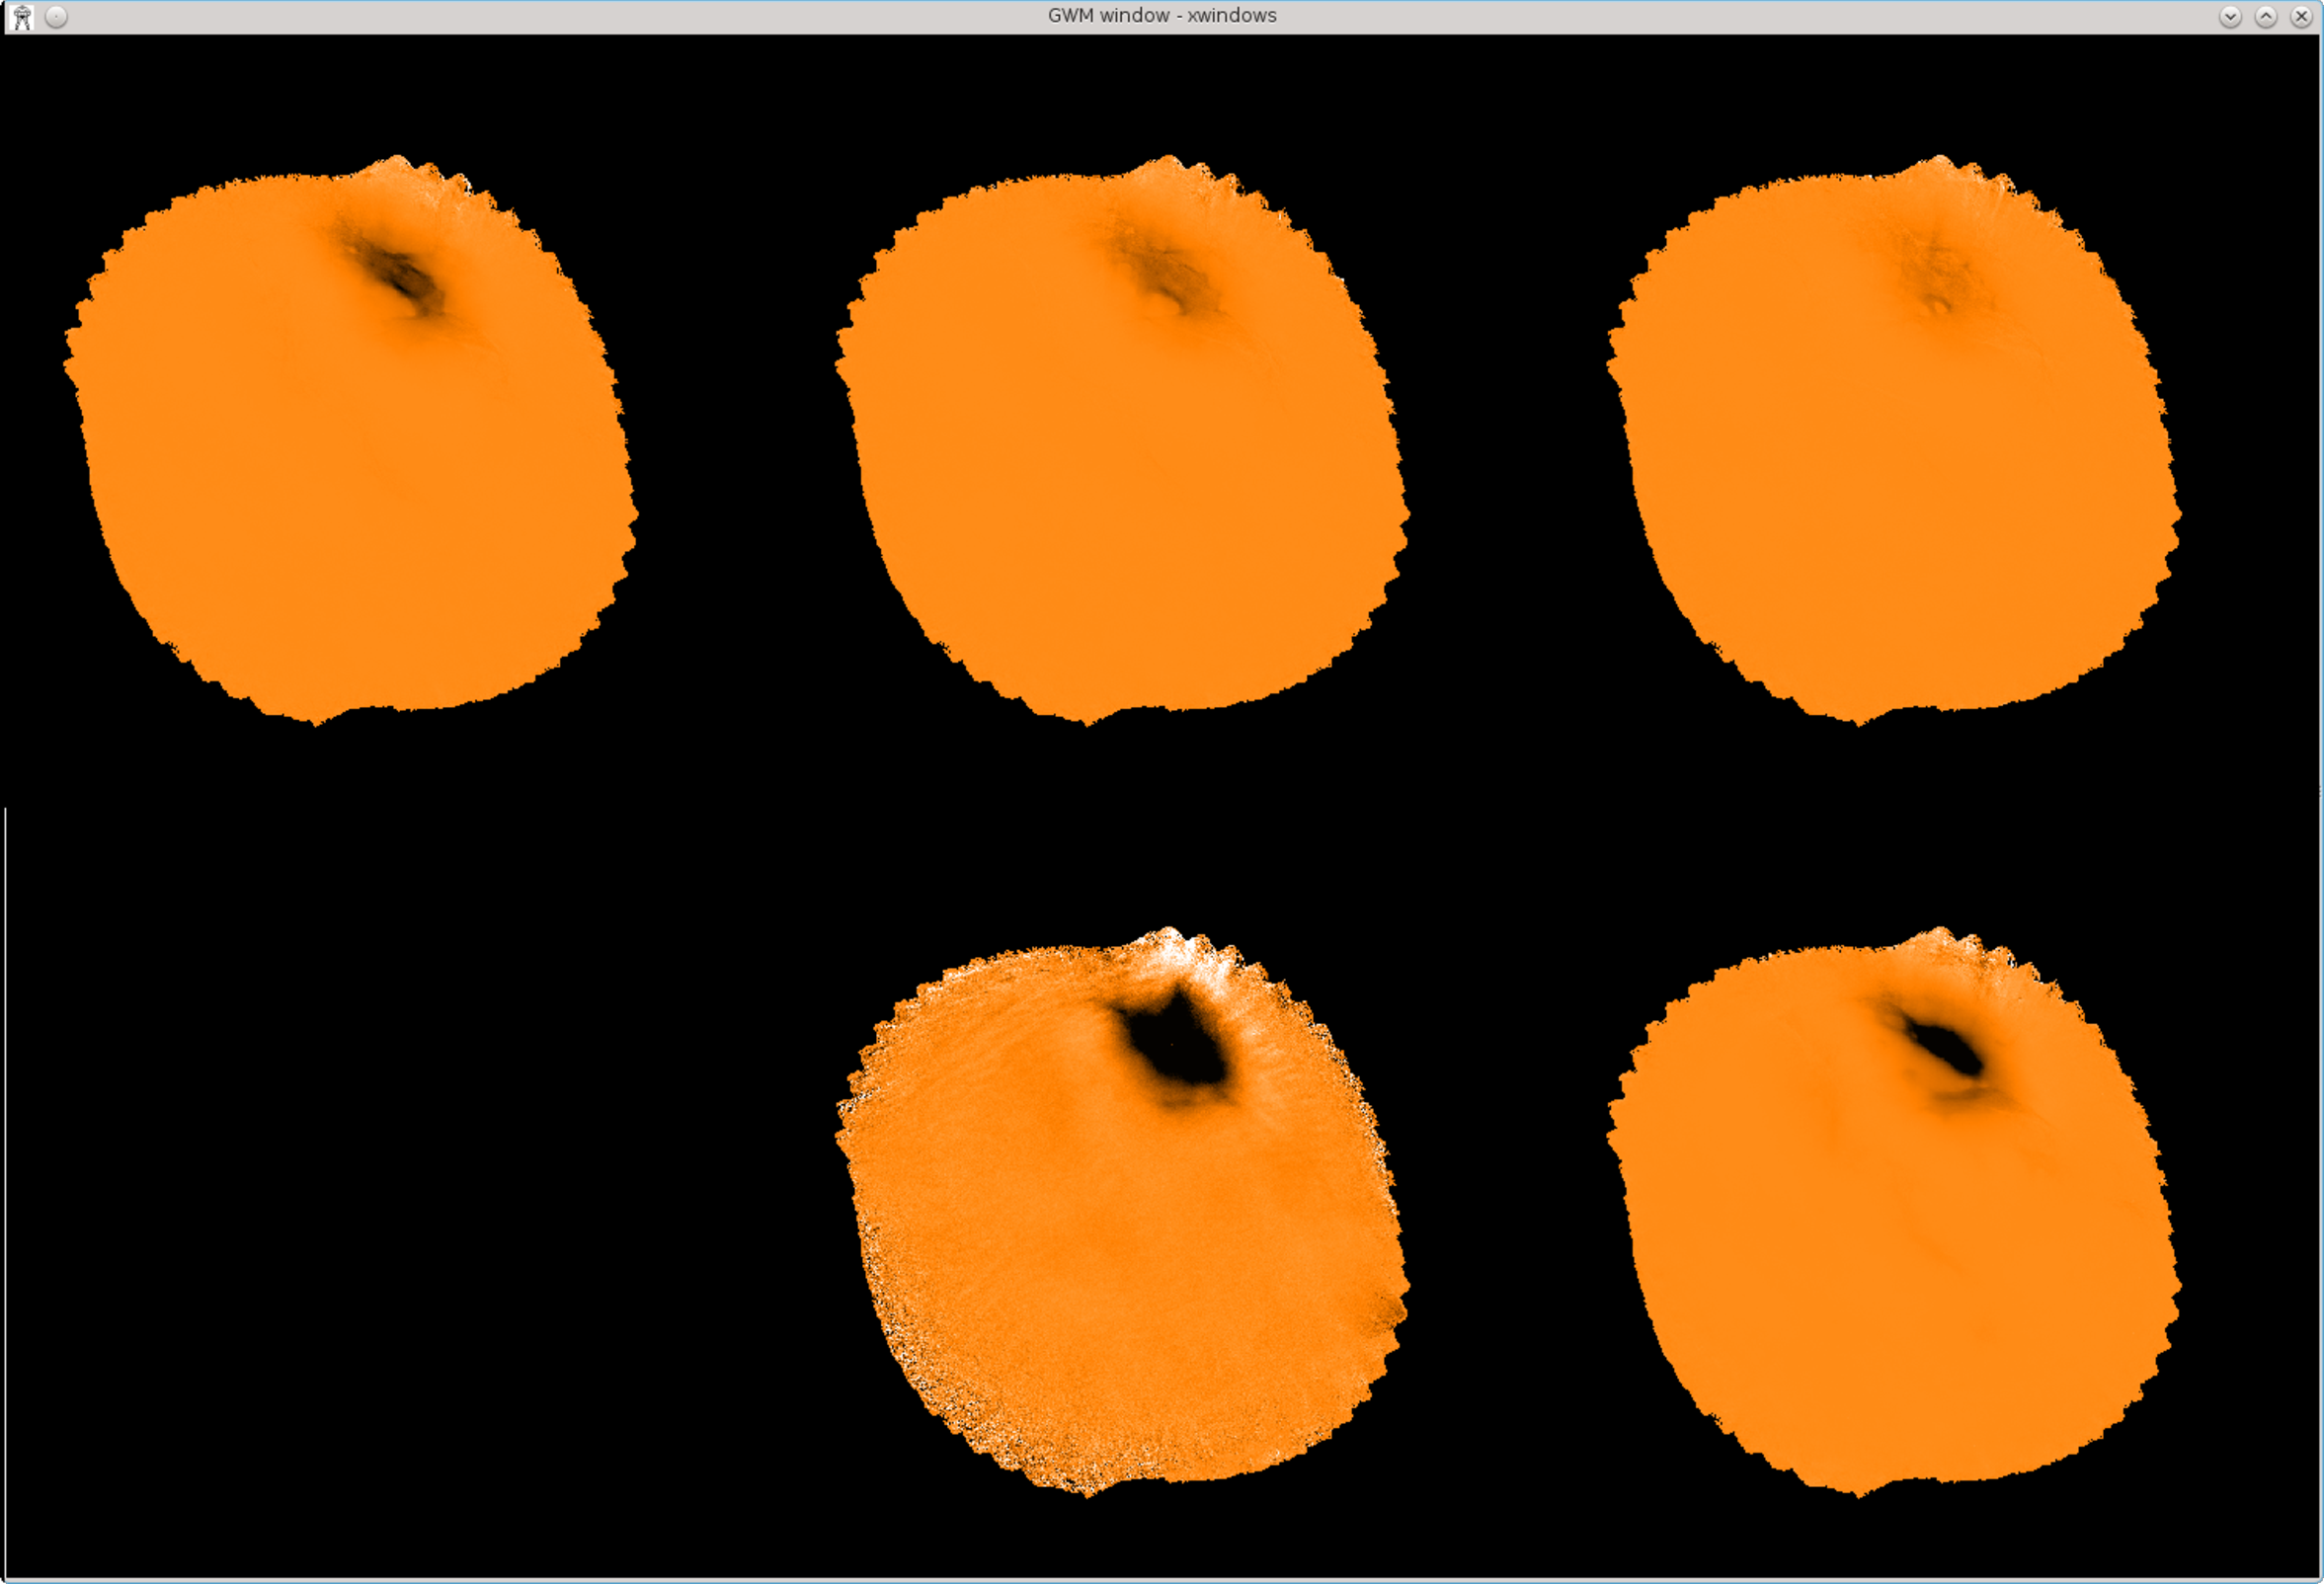
\includegraphics[width=\linewidth]{sc21_diffmaps}
\end{center}
\caption[Initial six difference maps]{\small The difference between each
pair of adjacent maps shown in \cref{Figure}{fig:itermaps}{Initial
six itermaps}.}
\label{fig:diffmaps}
\end{figure}

\textbf{Viewing the mask after each iteration:}

The above plots are based on the itermaps that are created by adding
``\texttt{itermaps=1}'' to your \texttt{makemap} configuration. You can
instead use ``\texttt{itermaps=2}'', which causes each itermap to be
masked so that pixels outside the current source mask are set bad
(\emph{i.e.} blank)\footnote{If no masking is being used, then
\texttt{itermaps=2} has the same effect as \texttt{itermaps=1}.}.
\cref{Figure}{fig:maskeditermaps}{Initial six itermaps with masking}
shows the resulting itermaps.

\begin{figure}
\begin{center}
  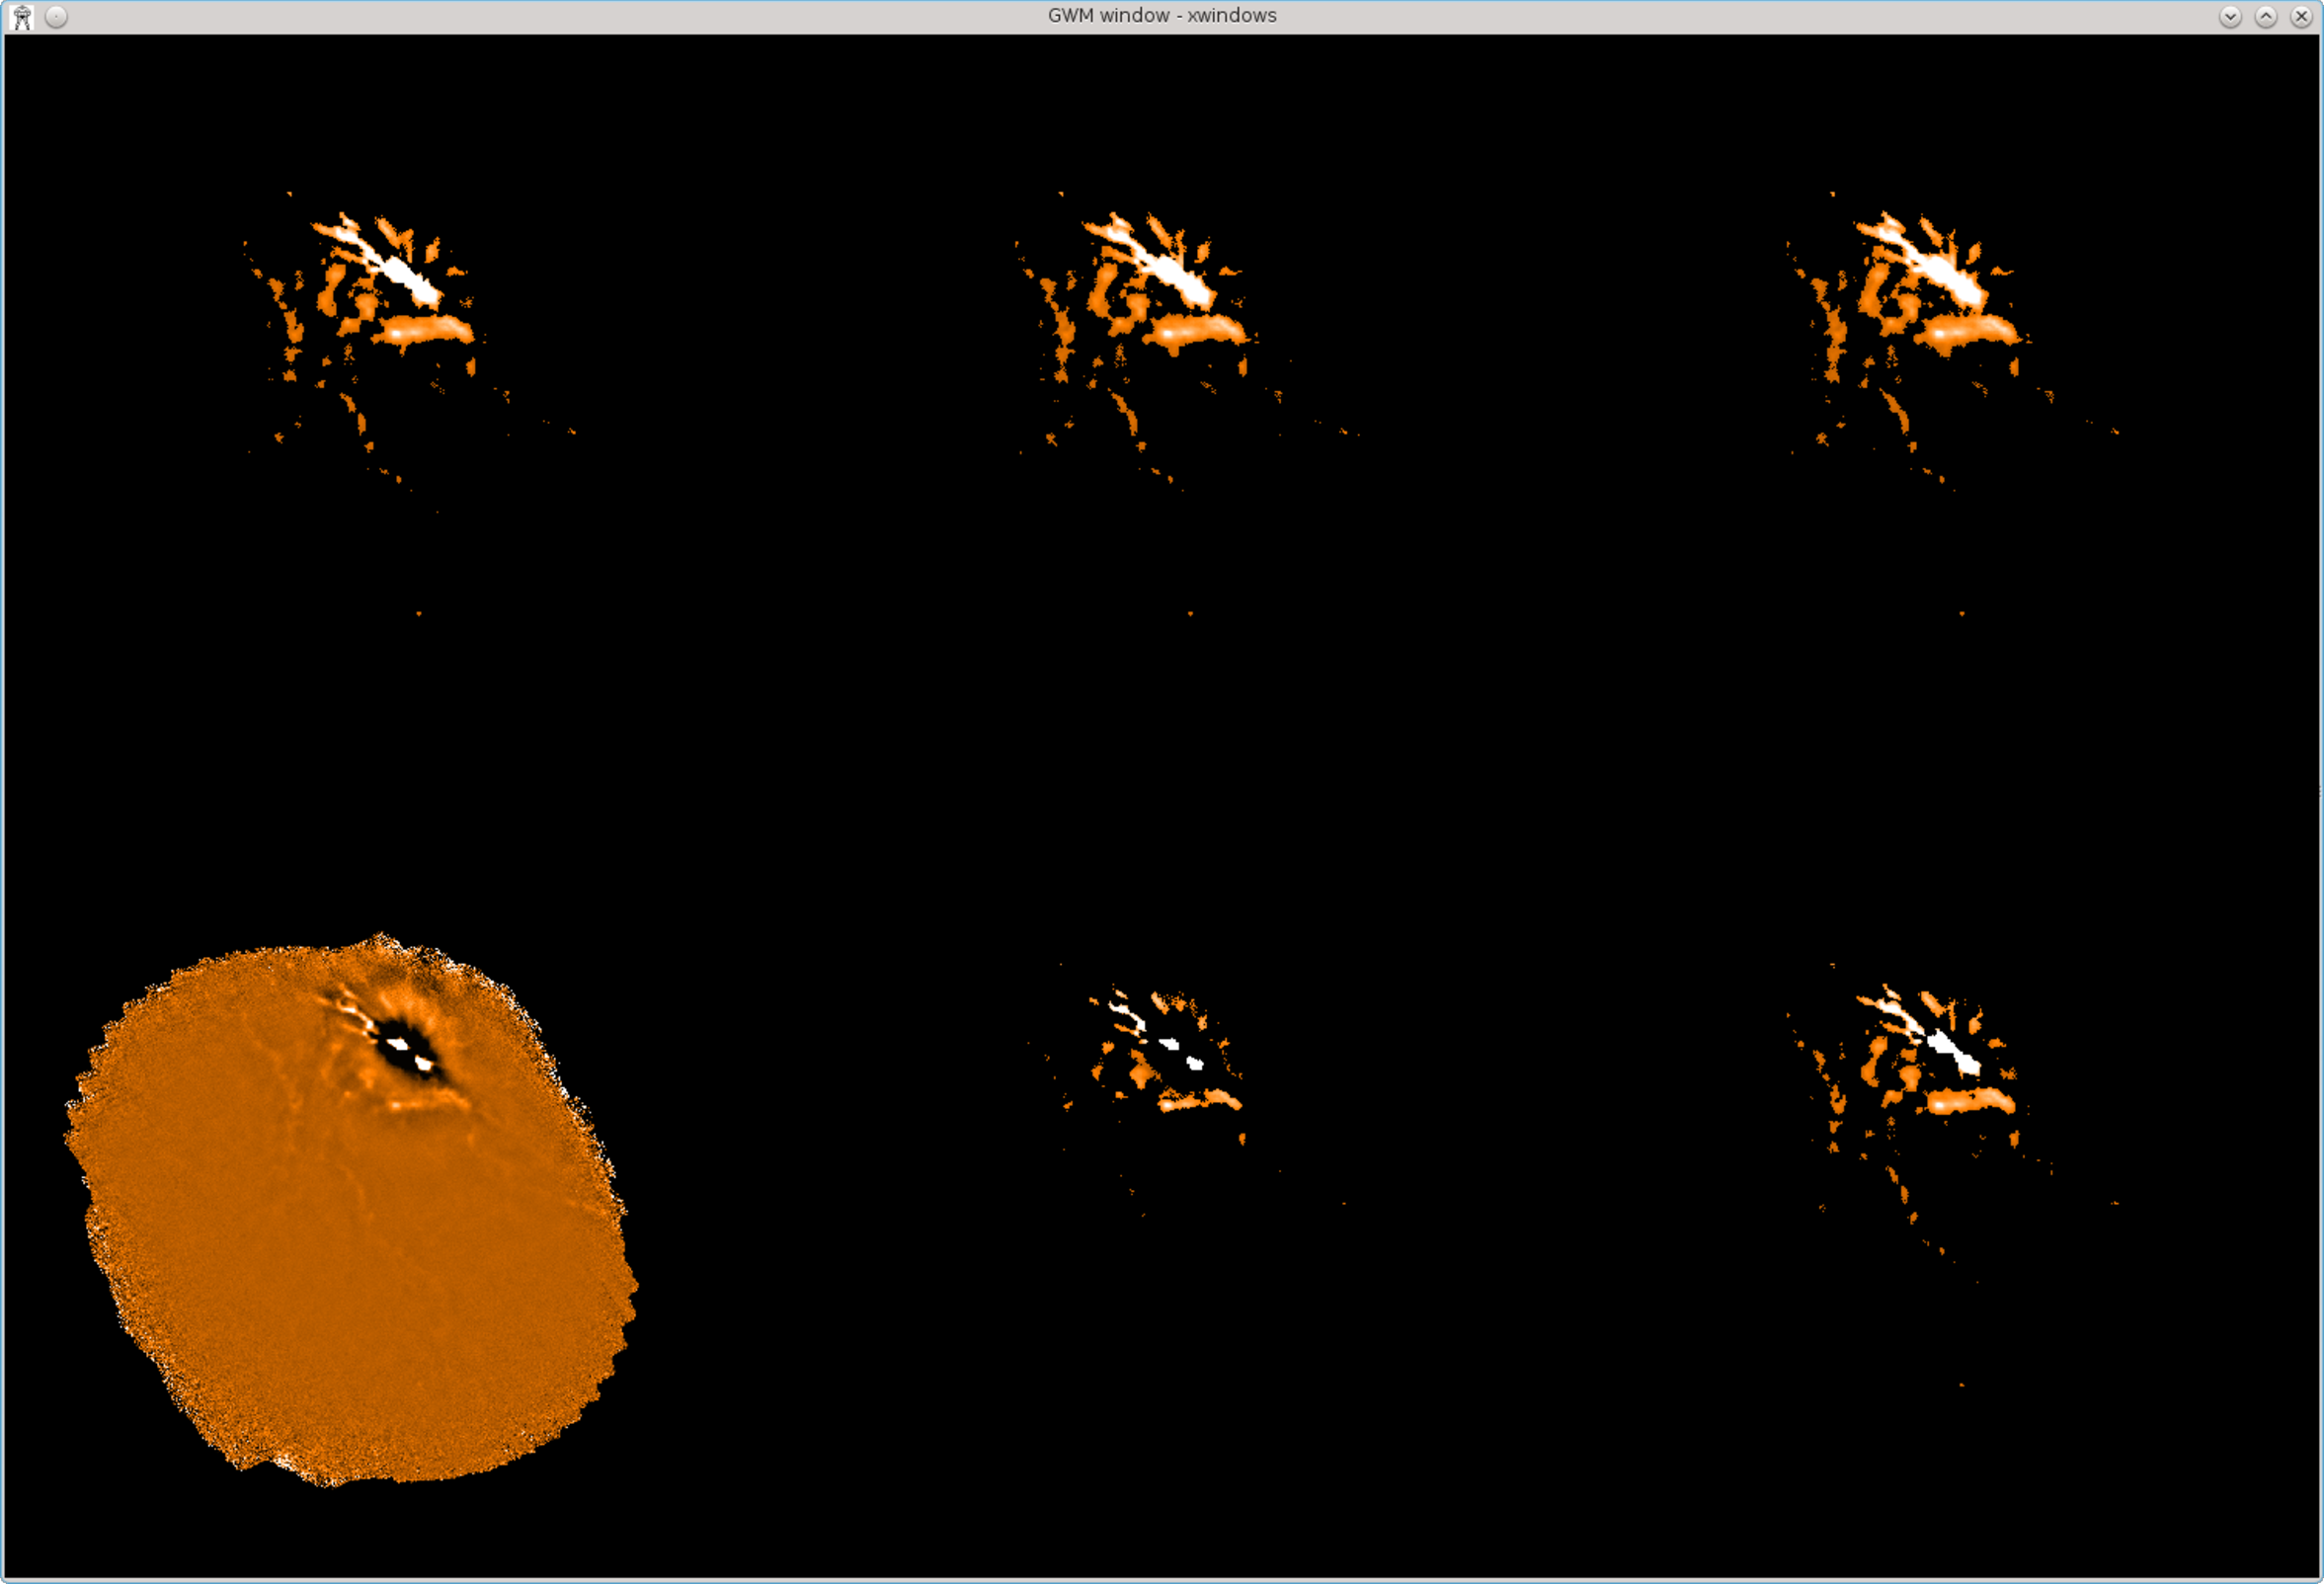
\includegraphics[width=\linewidth]{sc21_itermaps_masked}
\end{center}
\caption[Initial six itermaps with masking]{\small The first six
itermaps, create by using \texttt{itermap=2} in the configuration. This
causes pixels outside the source mask to be set blank, allowing the evolution
off the mask to be seen (the first iteration is not masked). In this
case, the mask includes all pixels above a signal-to-noise ratio of five.}
\label{fig:maskeditermaps}
\end{figure}

The main point of this section is to emphasise that all the above
investigations can be performed \emph{whilst makemap is still running},
if you specify an explicit file for the itermaps using the
``\texttt{itermaps} command-line option. This allows you to decide if
the reduction is progressing as expected, and whether to interrupt the
reduction.


\subsection{Interrupting \texttt{makemap}}

If you interrupt \makemap\ by pressing control-C on the keyboard (or
equivalently by sending an \texttt{INT} signal to the \texttt{makemap}
process), it will continue until the current iteration is completed
and then will issue a prompt with options allowing you to save the current
map before closing, as in the following example:

\begin{terminalv}
% makemap in=^infiles out=outmap config=^conf itermaps=myitermaps
Out of 29 input files, 1 was a dark, 1 was a fast flat and 27 were science
Processing data from instrument 'SCUBA-2' for object 'OMC1 tile10' from the
following observation  :
...
...
\end{terminalv}

\texttt{<press control-C>}

\begin{terminalv}
...
...
--- Quality flagging statistics
--------------------------------------------
 BADDA:   25525734 (20.86%),         267 bolos  ,change          0 (+0.00%)
BADBOL:   31261854 (25.55%),         327 bolos  ,change          0 (+0.00%)
 SPIKE:        339 ( 0.00%),                    ,change          4 (+1.19%)
DCJUMP:     146703 ( 0.12%),                    ,change          0 (+0.00%)
  STAT:     160000 ( 0.13%),         125 tslices,change          0 (+0.00%)
   COM:    1827454 ( 1.49%),                    ,change       3000 (+0.16%)
 NOISE:    5640518 ( 4.61%),          59 bolos  ,change          0 (+0.00%)
Total samples available for map:   89135553, 72.84% of max (932.361 bolos)
     Change from last report:      -3001, -0.00% of previous
smf_iteratemap: *** CHISQUARED = 0.998314983615372
smf_iteratemap: *** change: -0.0014711436109287
smf_iteratemap: *** NORMALIZED MAP CHANGE: 0.00941492 (mean) 2.9521 (max)


>>>> Interrupt detected!!! What should we do now? Options are:
1 - abort immediately with an error status
2 - close the application returning the current output map
3 - do one more iteration to finalise the map and then close

NOTE - another interrupt will abort the application, potentially leaving
files in an unclean state.

INTOPTION - What to do now (1-3) /3/ >
\end{terminalv}

At this point you should respond to the prompt for parameter
\texttt{INTOPTION} by typing 1, 2 or 3 followed by \texttt{<return>}. Options 2
and 3 cause \texttt{makemap} to tidy up its internals and create a map
from the current models just as if the iterative process had reached
convergence. Option 3 causes one further iteration to be performed,
without masking (you should use this option if you have been using AST
masking --- see \cref{Section}{sec:astmask}{AST masking}).

\begin{tip}
Note if you are running \texttt{makemap} from within a script, then the
handling of control-C interrupts will probably be quite different, because
the shell process (or perl, python or whatever) will catch the interrupt
before it gets to the \texttt{makemap} process. This usually causes the
shell process to die but leaves the \texttt{makemap} process running in
the background. Instead of pressing control-C on the keyboard, you should
find the process ID for the \texttt{makemap} process itself, and then send an
INT signal to that process explicitly:

\begin{terminalv}

% ps aux | grep makemap
dsb      25407  0.0  0.0  43716  1952 pts/5    0:00 makemap
% kill -s INT 25407

\end{terminalv}

\end{tip}


\section{Tips and Tricks}
\subsection{Aligning your map with a pre-existing image}
If you want to compare SCUBA-2 data with a map of the same region taken
with a different instrument, you will usually want to create the
SCUBA-2 map using the same pixel grid as the other map so that you can
compare pixel values directly in the two maps\footnote{Creating the map on the
required pixel grid is better than creating it on a default grid and then
re-sampling it onto the required grid later.}. You can use the
\aparam{REF} command-line parameter to do this. For instance, if your
other map is in file \texttt{herschel.sdf}, you can do:

\begin{terminalv}
% makemap in=^infiles out=outmap config=^conf ref=herschel
\end{terminalv}

This will cause the output map in file \texttt{outmap.sdf} to use
the same pixel grid as \texttt{herschel.sdf}.  This means that a given
point on the sky will have the same \emph{pixel coordinates} in both
maps, and so for instance you could divide one by the other to get a
ratio map without any further alignment step:

\begin{terminalv}
% div outmap herschel ratio_map
\end{terminalv}

This will divide \texttt{outmap.sdf} by \texttt{herschel.sdf} and put the
ratio in \texttt{ratio\_map.sdf}\footnote{In reality you would probably
want to take account of differing resolutions and /or units in the two
maps before dividing them.}.

However, by default \texttt{makemap} will trim the output map to
exclude blank borders, thus the two maps may have different
\emph{dimensions}. NDF-based applications such as \textsc{Kappa}
\xref{\task{div}}{sun95}{DIV} automatically take account of this when
comparing corresponding pixels in two NDFs --- see
\cref{Figure}{fig:pixelco}{Pixel coordinates}.

\begin{figure}
\begin{center}
  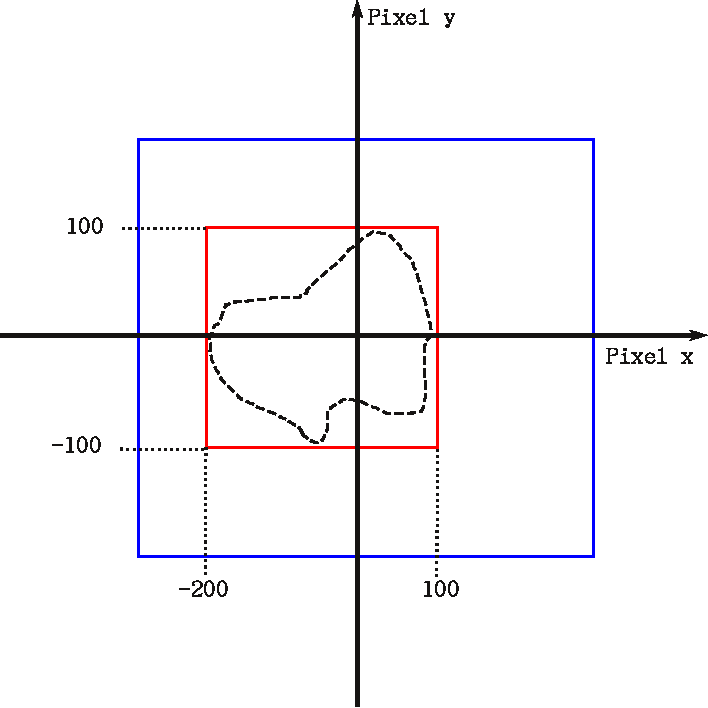
\includegraphics[width=0.8\linewidth]{sc21_pixelco}
\end{center}
\caption[Pixel coordinates]{\small The curved dotted line represents a
contour of an astronomical object. The heavy black lines represent the
X and Y axes of the pixel coordinate system, crossing at the pixel origin
(\texttt{pixel\_x},\texttt{pixel\_y})=(0,0). The numerical values
represent pixel X and Y values. The blue box represents the
bounds of the reference map supplied when running makemap. The
red box represents the bounds of the map created by makemap.
The reference image and the output image share the same pixel
coordinate system, so a given point on the sky has the same pixel
coordinates in both images. However, the output (red) image is cropped to
remove blank borders and so has smaller dimensions than the reference
(blue) image. All this is made possible by the fact that the NDF format, unlike
FITS, does not require the origin of pixel coordinates to be at the
bottom left corner of each map. NDF applications account for any
difference in pixel origin when comparing pixels in different files.}
 \label{fig:pixelco}
\end{figure}

If you want to force the output map to have certain bounds in pixel
coordinates, you can do so by assigning values to the \aparam{LBND} and
\aparam{UBND} parameters when running \texttt{makemap}. For instance, if
you want to force the output map to have the same dimensions as the
reference map, you could use \textsc{Kappa} \xref{\task{ndftrace}}{sun95}{NDFTRACE}
to list the properties of the reference NDF, including its pixel bounds, and
then assign these bounds to \aparam{LBND} and \aparam{UBND} parameters when
running \texttt{makemap}:

\begin{terminalv}
% ndftrace herschel

   NDF structure /home/dberry/herschel1:
      Title:  Example Herschel data

   Shape:
      No. of dimensions:  2
      Dimension size(s):  351 x 400
      Pixel bounds     :  -50:300, 1:400
      Total pixels     :  140400
...
...
% makemap in=^infiles out=outmap config=^conf ref=herschel \
          lbnd=\[-50,1\] ubnd=\[300,400\]
\end{terminalv}

The resulting map in \texttt{outmap.sdf} will have the same pixel bounds
as \texttt{hershel.sdf}.

\subsection{Limiting the amount of memory used by \texttt{makemap}}
There may be occasions when you need to limit the amount of memory used
by \makemap\ --- for instance to leave enough memory for other processes
to function correctly. For machines with more than 20 GB of memory, the
default is to leave 4 GB free for other processes. For machines with less
than than 20 GB of memory, the default is to leave 20\% of the total
memory free. This default can be over-ridden by indicating the maximum
amount of memory that \texttt{makemap} should use by setting a value for
the command-line parameter \aparam{MAXMEM}. For instance:

\begin{terminalv}
% makemap in=^infiles out=outmap config=^conf maxmem=50000
\end{terminalv}

will ensure that \texttt{makemap} never uses more than 50000
MiB\footnote{One MiB is 1048576 bytes.} of memory. Be aware though that
for larger observations this may cause the data to be processed in
multiple chunks rather than a single continuous chunk, resulting in a
poorer map.

\subsection{Re-using previously cleaned data to speed up map-making}

Usually, you will create your SCUBA-2 maps using one of the standard
configuration files distributed with \textsc{smurf} (see
\cref{Section}{sec:config} {Specialised configuration files}). However,
for certain problematic observations it may sometimes be necessary to
experiment with several different configurations to find one that
produces an acceptable map. In such cases a significant amount of time
can be saved by re-using pre-cleaned raw data each time you make a map,
rather than re-cleaning it each time.

By default \makemap\ assumes that the supplied data is raw data that
requires cleaning before being used to make a map. However, if you include
``\setparam{DOCLEAN}{doclean}{0}'' in your configuration, then
\texttt{makemap} will skip the entire cleaning process and move directly
on to the iterative map-making stage, thus saving significant time.

Obviously though, in this case you need to make sure that the data you
supply to \texttt{makemap} has already been cleaned. There are two ways
to do get cleaned data:

\begin{enumerate}

\item You can run \texttt{makemap} initially on the \emph{un}-cleaned
data (\emph{i.e.} the original raw data), and force \texttt{makemap} to
dump the cleaned data to disk before going onto the iterative map-making
stage. You can then re-use this cleaned data in subsequent invocations of
\texttt{makemap}. To dump the cleaned data, you need to add
``\setparam{EXPORTCLEAN}{exportclean}{1}'' to the configuration on your
initial run of \texttt{makemap} --- don't forget to remove it for
subsequent runs! The cleaned data are put into files in the current
directory, one for each sub-array, with names such as
\texttt{s8c20120706\_00037\_0003\_con\_res\_cln.sdf}. Note the \texttt{\_cln} on
the end of the name indicating cleaned data. The base name,
``\texttt{s8c20120706\_00037\_0003}'' in this case, is taken from the first
raw data file that contributes to each chunk. If the entire observation
is processed in one chunk (as it should usually be) then there will be
one such \texttt{\_cln} file for each sub-array. If the observation is
split into multiple chunks, then there will be multiple  \texttt{\_cln} files
for each sub-array (one for each chunk).

\item You can use the separate \smurf\ task \clean\ to clean the data
as described in \cref{Appendix}{app:clean}{Cleaning the raw data}.

\end{enumerate}






\newpage
\chapter{\xlabel{tweak}Tailoring Your Reduction}
\label{sec:tweak}


\section{Adding and amending parameters}
The configuration file \file{dimmconfig\_jsa\_generic.lis} is a good
configuration file to use as a first pass for reducing any data, and is
the default configuration used by the pipeline's \drrecipe{REDUCE\_SCAN}
recipe.

\textbf{You can create your own personalised configuration file from
scratch or copy one of the provided ones to your local directory and
edit it.}

The first line of each specialised configuration file is often the path
to another configuration file --- known as the \emph{parent} configuration
file. The new configuration file inherits all the parameter values
defined by the parent configuration file, and then goes on to specify
additional parameter settings which may supplement or over-ride those
defined in the parent configuration file. Parameters that are not set to
a specific value by \emph{either} configuration file assume the default
values listed in \cref{Appendix}{app:parameters}{Configuration-parameter
descriptions}\footnote{These default values are defined in the file
\texttt{\$SMURF\_DIR/smurf\_makemap.def}.}.

Often you will want to use one of the pre-defined configuration files
included within \starlink\ tree as the parent configuration. Remember
that any parameters appearing in your configuration file
automatically override the values supplied by the parent file. As an
example, consider the following text file ``\texttt{myconf}'':

\begin{terminalv}
% cat myconf

#  This is an example configuration file.
^$STARLINK_DIR/share/smurf/dimmconfig_jsa_generic.lis

numiter=-100
maptol=0.01

\end{terminalv}

The first thing to note is that blank lines and comment lines
(\emph{i.e.} lines beginning with the hash character ``\texttt{\#}'') are
ignored and can be used to document your configuration file. Next note
that this example file uses
\texttt{\$STARLINK\_DIR/share/smurf/dimmconfig\_jsa\_generic.lis} as its
parent (the path to the parent file must be preceded
by an up-caret (\texttt{\^}) character). Thus, all the parameter values
set by \texttt{\$STARLINK\_DIR/share/smurf/dimmconfig\_jsa\_generic.lis} are
first read, before adding in other parameter settings. In this case, values
are assigned to \param{maptol} and \param{numiter}, over-riding the
values provided by the parent file.

You can use more than one parent file if required (each one a separate
line, and preceded by an up-caret). Each specified parent will be read in
turn, with parameter settings read from later ones having priority over
those read from earlier ones.

You can also add or amend parameters by listing them directly on the
command line. They are appended to the configuration file name as a
comma separated list as shown in the example below. Be sure to include
all the necessary quotation marks.

\begin{terminalv}
% makemap in='s8*.sdf' out=850map method=iterate \
config='"^dimmconfig\_jsa\_generic.lis,numiter=-50,exportndf=(flt,noi),itermap=1"'
\end{terminalv}

For full details of all the possible ways of specifying groups of
parameter values, see Section ``\xref{Specifying Groups of
Objects}{sun95}{se_groups}'' in ``\xref{Starlink User Note 95}{sun95}{}.

\textbf{What parameters can be changed?}\\*
\cref{Appendix}{app:parameters}{Configuration-parameter descriptions}
lists the parameters that are more likely to be of interest to you when
creating your own configuration files. You can also change any of the
other more esoteric parameters not included in that list --- see
Appendix \xref{SUN/258} {sun258}{par_full} within \xref{Starlink
User Note 258}{sun258}{} for a full list -- but we do not advise this.

\begin{tip}
  If some feature is switched on either by default or within
  the parent configuration file, it can be switched off if required
  by assigning a suitable value to the corresponding parameter within
  your own configuration file. The value needed to do this will be
  given in the parameter description in \cref{Appendix}{app:parameters}
  {Configuration-parameter descriptions} --- for instance it may be
  \param{<undef>}, or \param{0}, or some other special value.
\end{tip}

\textbf{Note:} any parameter can be made wavelength dependent by
adding the prefix \param{450.} or \param{850.}, e.g.
\param{flt\_edge\_largescale} applies to both 450\,$\mu$m and
850\,$\mu$m whilst \param{450.flt\_edge\_largescale} applies to
450\,$\mu$m only. Be aware that if both are specified, unqualified
values (no prefix) take priority over qualified values.

\section{\xlabel{inter}Writing out models \& intermediate maps}
\label{sec:inter}

\textbf{itermaps}\\
Setting the parameter \setparam{ITERMAP}{itermap}{1} writes out the
map containing the astronomical signal after each iteration. Setting
\param{itermap~=~2} adds the QUALITY component.  These can be visually
inspected with

\begin{terminalv}
% gaia 850map.more.smurf.itermaps
\end{terminalv}

to help determine an appropriate number of iterations. Alternatively, you
can view several itermaps simultaneously side-by-side (\emph{e.g.}
\cref{Figure}{fig:itermaps}{Initial six itermaps}) using \Kappa\ as
described in \cref{Section}{sec:itermaps}{Monitoring the map at the
end of each iteration}.

Viewing itermaps is useful when a fixed number of iterations have been requested (i.e. a positive
value for \xparam{NUMITER}{numiter}) and the map solution diverges before
they have completed. See also \cref{Section}{sec:itermaps}{Monitoring the map
at the end of each iteration} for how to view these maps whilst \makemap\ is still running.
\newline\newline
\textbf{shortmaps}\\
If the parameter \param{shortmaps} is non-zero, a map is made from
every group of adjacent time-slices (as specified by the parameter).
These are stored as an NDF extension and can be viewed \gaia.

\begin{figure}[ht!]
\begin{center}
\begin{fmpage}{0.95\linewidth}
\vspace{0.2cm}
\hspace{2mm}
\textbf{Viewing ITERMAPs}
\minipageclear
\vspace{0.5cm}

\begin{minipage}[c]{0.65\linewidth}

\begin{terminalv}
% stackframes map.more.smurf.itermaps \
sort=false map_itermaps
\end{terminalv}
\end{minipage}
\hspace{0.3cm}
\begin{minipage}[c]{0.29\linewidth}
Stack the individual itermaps into a single cube (\textsc{Kappa}
\xref{PASTE}{sun95}{paste} can also be used).
\end{minipage}
\minipageclear

\vspace{0.5cm}

\begin{minipage}[c]{0.65\linewidth}
\centering
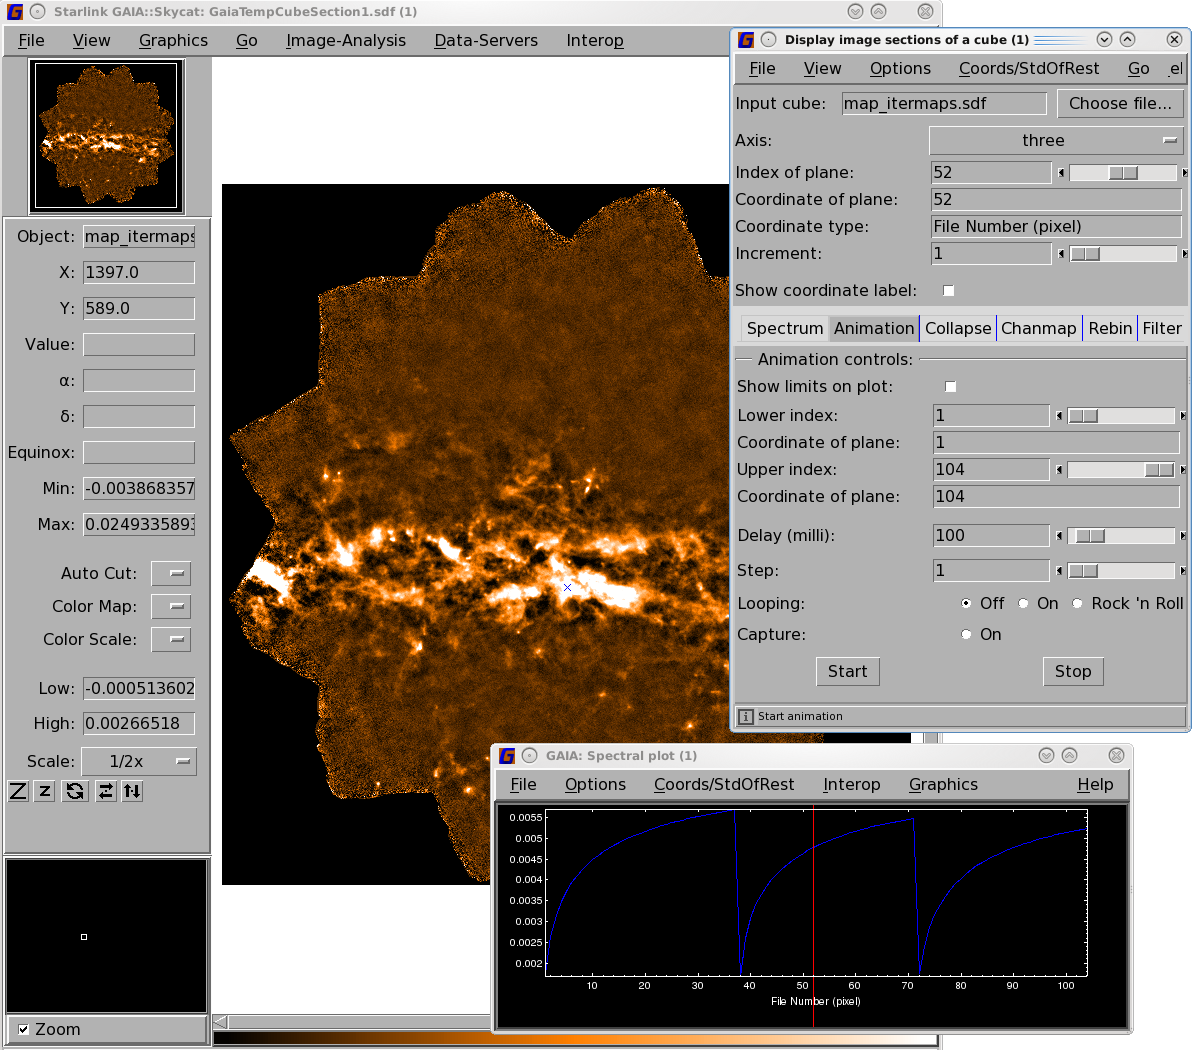
\includegraphics[width=0.95\textwidth]{sc21_itermaps_anim}
\end{minipage}
\hspace{0.3cm}
\begin{minipage}[c]{0.29\linewidth}
The output map \file{map\_itermaps} can be opened with \gaia. The data used
in this example is the Galactic map reduced in
\cref{Section}{sec:bright_ex}{\file{dimmconfig\_bright\_extended.lis}}. The
Spectral plot window shows the value for a single pixel and the three
chunks are easily identified. You can select the \gaiathing{Animation} tab
in the \gaiathing{Display image sections} window and click
\gaiathing{Start} to loop through the itermaps for each iteration.  The
`movie' will appear in the main \gaia\ window.
\end{minipage}
\minipageclear

\vspace{0.7cm}

\begin{minipage}[c]{0.65\linewidth}
\centering
\hspace{0.5mm}
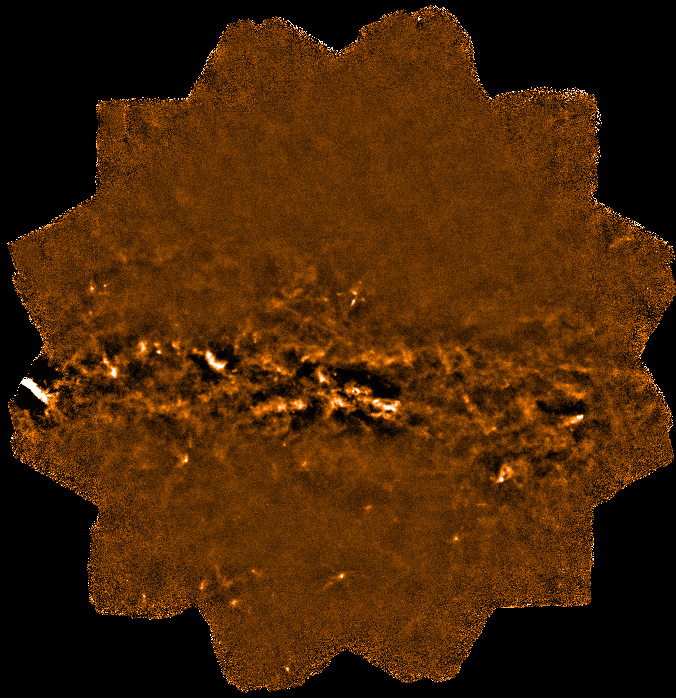
\includegraphics[width=3cm, ]{sc21_iter1}
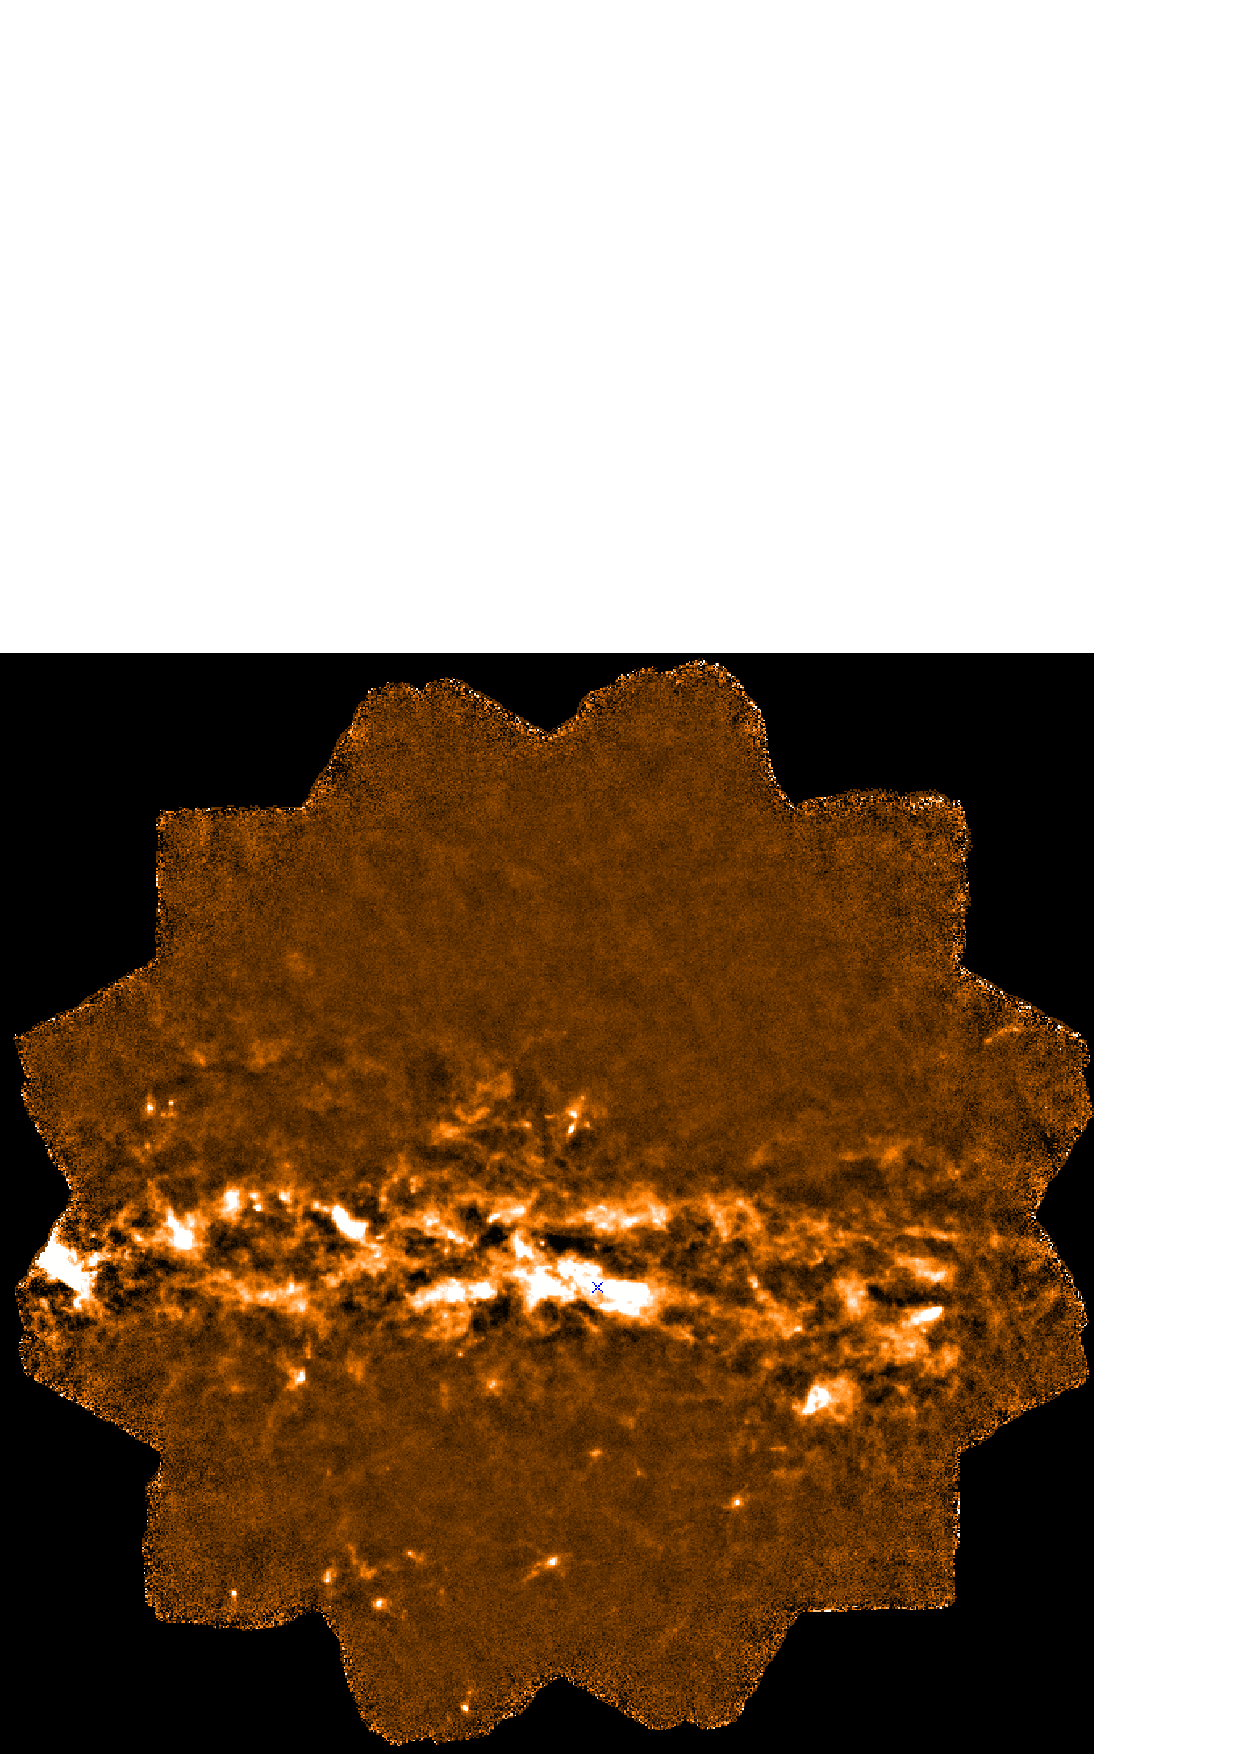
\includegraphics[width=3cm, ]{sc21_iter2}
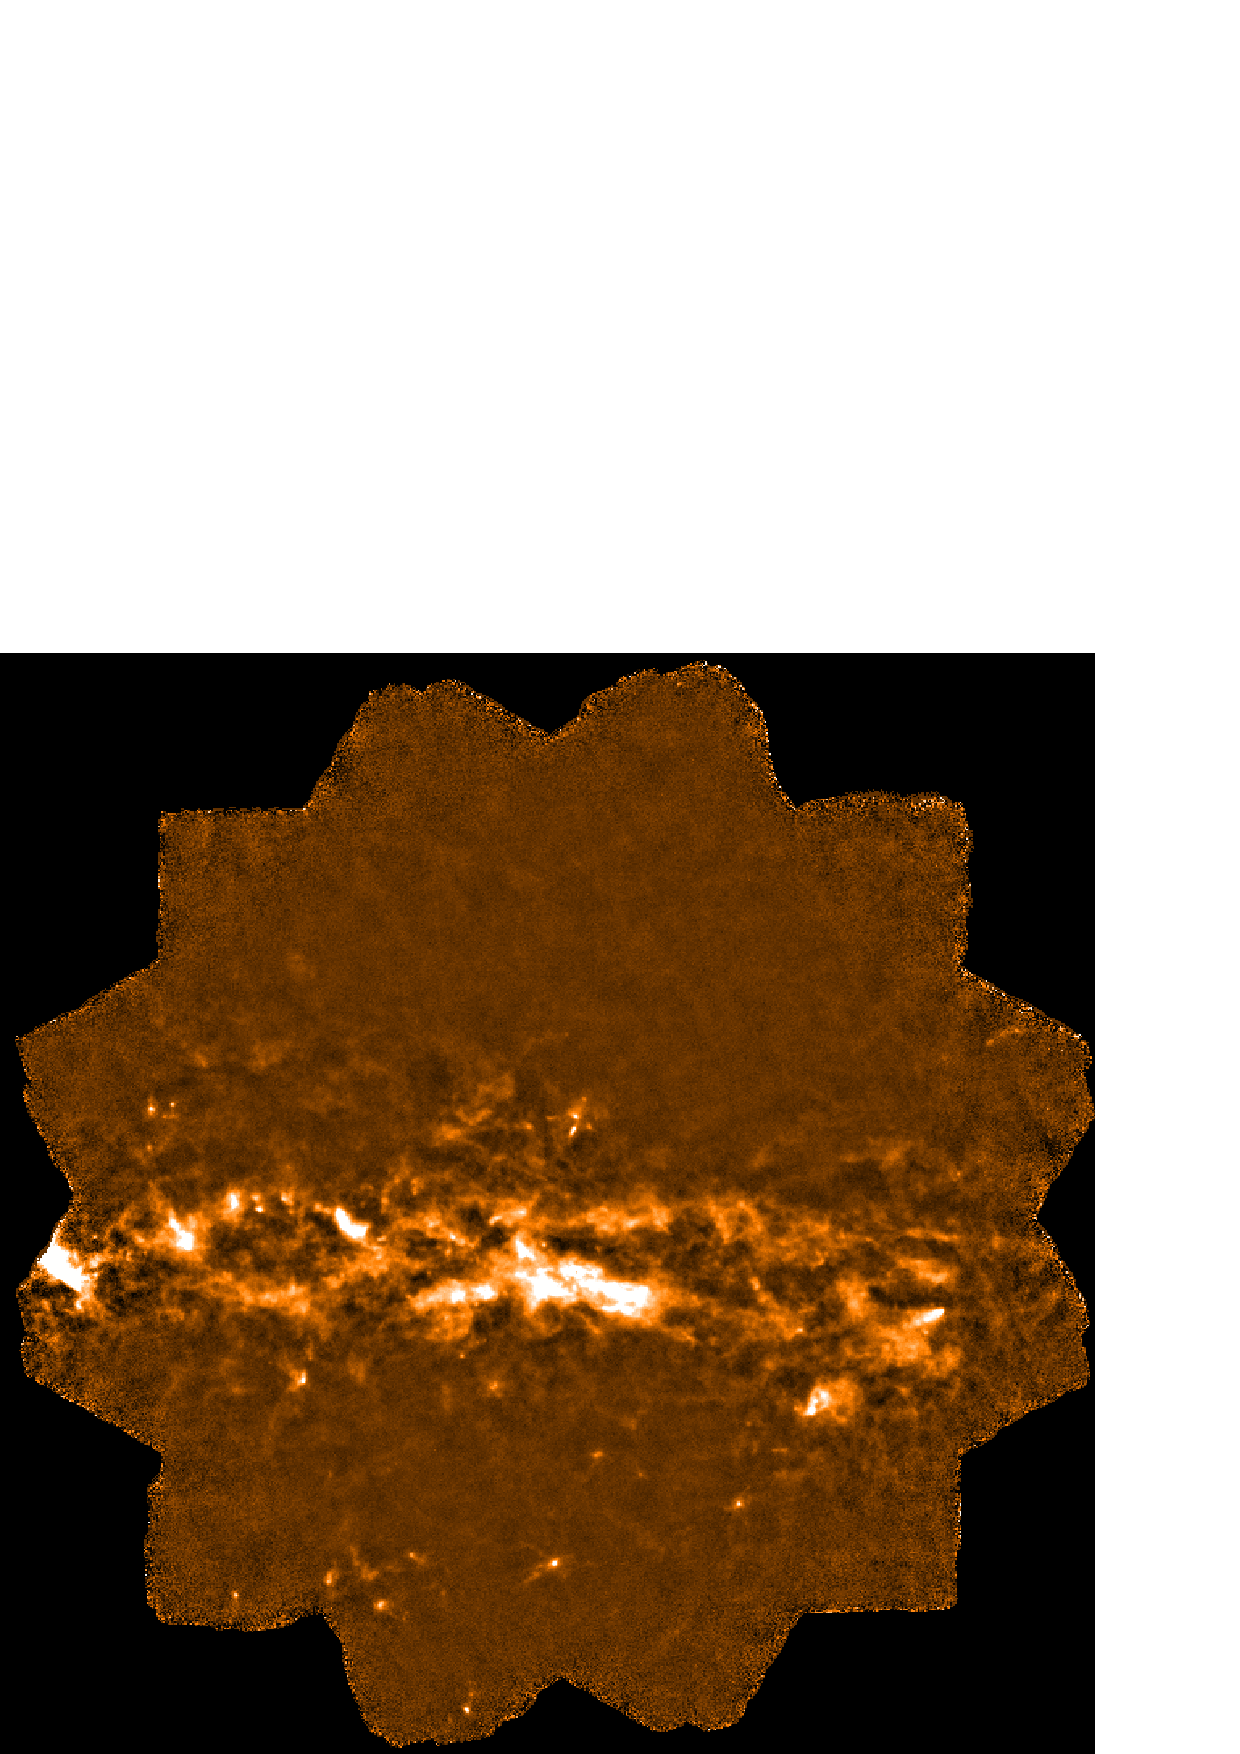
\includegraphics[width=3cm, ]{sc21_iter31}
\vspace{0.2cm}
\end{minipage}
\hspace{0.3cm}
\begin{minipage}[c]{0.29\linewidth}
These windows show the itermaps map at 1, 10, and 30 iterations. A
specific iteration can be selected using the \gaiathing{Index of plane}
slider on the \gaiathing{Display image sections} window.
\vspace{0.2cm}
\end{minipage}
\minipageclear
\end{fmpage}
\end{center}
\caption[View maps for each iteration]{
  \small Example using the \smurf\ command \stackframes\ and
  \gaia\ to view the `itermap' for each iteration.
}
\label{fig:stack}
\end{figure}


\begin{terminalv}
% gaia 850map.more.smurf.shortmaps
\end{terminalv}

You can view the shortmaps and itermaps more
conveniently by stacking them into a single cube using the \smurf\
command \stackframes. This cube can then be viewed as a
`movie' with \gaia, using the animation option to loop through the
itermaps. See \cref{Figure}{fig:stack}{the box above} for instructions.
\newline\newline
\textbf{exportmodel}\\
This parameter has been discussed in
\cref{Section}{sec:export}{Exporting individual models} and allowed
you to see the model that was fit for each component specified by the
\xparam{MODELORDER}{modelorder} parameter.

\section{\xlabel{filt}Large-scale filtering}
\label{sec:filt}

Some of the most important parameters to experiment with are the
filtering options. By default, no filtering is applied during the
pre-processing stage\footnote{However, the \blankfield\ configuration
over-rides this default.} (see \xparam{FILT_EDGE_LARGESCALE}{filt\_edge\_largescale}
and \xparam{FILT_EDGE_SMALLSCALE}{filt\_edge\_smallscale}). A high-pass
filter is used during the iterative stage if \xparam{MODELORDER}{moelorder}
includes \model{FLT}\footnote{The \blankfield\ configuration omits
\model{FLT} from \param{modelorder}.}, and selected a suitable value
for the filter size is crucial for maps containing extended emission.

The maximum spatial scale of structure that can be recovered by the
map-maker is determined by the scanning speed and frequency cut
applied to the data:

\begin{equation}
\frac{\textrm{speed}[arcsec / \textrm{s}]}{\textrm{frequency
    cut}[\textrm{Hz}]}=\textrm{scale size}[arcsec]
\end{equation}

The default (\emph{i.e.} if no configuration is supplied) filter sizes
in arc-seconds are:

\setparam{FLT.FILT_EDGE_LARGESCALE}{450.flt.filt\_edge\_largescale}{200} \\
\setparam{FLT.FILT_EDGE_LARGESCALE}{850.flt.filt\_edge\_largescale}{480}.

To make your life easier, these parameters allow you to specify the
filter limits in terms of spatial scale in arc-seconds---in this case
480\,arcsec at 850\,$\mu$m and 200\,arcsec at 450\,$\mu$m. For example,
at 850\,$\mu$m, recovering scales of 480\,arcsec at a scan speed of
600\,arcsec/sec (default for a 1 degree \textsc{pong}) corresponds to
a frequency of 1.25\,Hz.

Choosing a high-pass filter is especially important for the recovery
of extended emission. The \brightextended\ configuration file sets
\setparam{FLT.FILT_EDGE_LARGESCALE}{flt.filt\_edge\_largescale}{480}
for both 450\,$\mu$m and 850\,$\mu$m. Be aware that increasing filter sizes
decreases the flatness of your background. A compromise must be made between
extended structure and the flatness of your map. See \cref{Figure}{fig:fltcompare}
{the figure below} for an illustration of the effect of
\xparam{FLT.FILT_EDGE_LARGESCALE}{flt.filt\_edge\_largescale} on your map.

The scanning speeds are fixed for a given observing mode; you can find
out the speed at which your data were taken from the
\texttt{SCAN\_VEL} keyword in the FITS header (see
\cref{Section}{sec:fitsheader}{Headers and file structure}).

%\pagebreak[4]
\textbf{Flattening the background}\\*
There is an option to reduce the noise in your background introduced by
setting a high value for the large-scale filter. The parameter
\xparam{FLT.FILT_EDGE_LARGESCALE_LAST}{flt.filt\_edge\_largescale\_last}
filters the regions outside your \model{AST} mask (see \cref{Section}
{sec:astmask}{AST masking}) on a shorter scale for the last iteration only,
thereby producing a much flatter background. Note that this is probably a
bad idea if you intend to co-add several observations, as it removes
potentially real structure in the background regions that could otherwise be
recovered by co-adding several observations. In general, use of
\param{flt.filt\_edge\_largescale\_last} should be seen as a cosmetic
enhancement, since it results in differing filter sizes being used inside
and outside the \model{AST} mask.

Also note that when using \param{flt.filt\_edge\_largescale\_last} the
variances stored in the final map are from the penultimate iteration in
order to avoid using the artificially reduced variances created on the
last iteration.

\begin{figure}
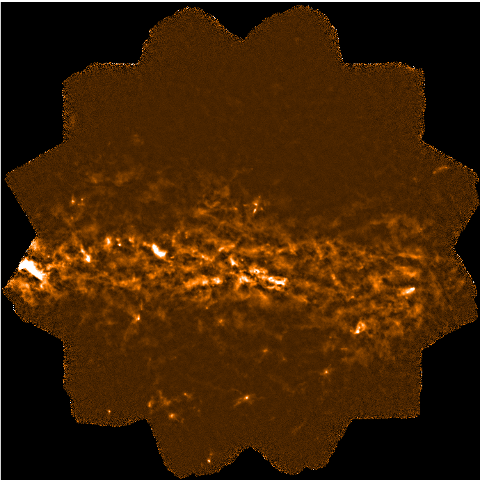
\includegraphics[width=0.46\linewidth]{sc21_brex_19}
\hspace{7mm}
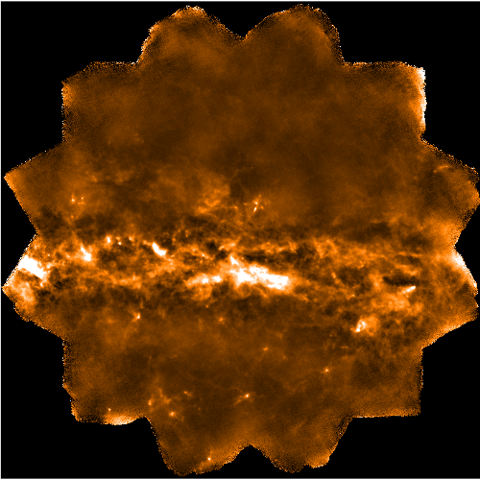
\includegraphics[width=0.46\linewidth]{sc21_brex_18}
\caption[Illustrating the effects of high-pass filtering]{
  Highlighting the effects of high-pass filtering on your map.
  \textbf{(Left)} Map made with \param{850.flt.filt\_edge\_largescale}{300}.
  \textbf{(Right)} Map made with \param{850.flt.filt\_edge\_largescale}{1000}.
  All other configuration parameters remain the same.\label{fig:fltcompare}
}
\end{figure}


\section{\xlabel{fitcom}Fitting COM for each sub-array}
\label{sec:fitcom}

A useful option to improve the flatness of your maps is to fit the
\model{COM} model independently for each sub-array. This is
particularly effective if you find you have one sub-array noisier than
the others.

This comes with the warning however that you will lose information on
any scales larger than the area covered by a single sub-array. It is
therefore not recommended if you have very large-scale extended
structure.

To initialise this option set \setparam{COM.PERARRAY}{com.perarray}{1}.


\section{\xlabel{noibox}Flagging bad data}
\label{sec:noibox}

Bolometers that have higher noise levels are down-weighted when forming
the map. By default, a separate noise estimate is created for each
15 second section\footnote{15 seconds is half a sub-scan.} of each bolometer
time-stream, but an alternative length can be specified using parameter
\xparam{NOI.BOX_SIZE}{noi.box\_size}.

Dividing each bolometer up into sections helps to remove `scuffs' or other
noise artefacts you might see in your error map due to a sub-array (or
arrays) temporarily jumping to a higher noise state. As the section length
tends to 1 second we find some of the source signal being down-weighted.
Higher than this 15 seconds and the map-maker becomes less sensitive to
the higher noise states.

Other parameters you may want to try include \xparam{FLAGFAST}{flagfast} and
\xparam{FLAGSLOW}{flagslow}. You may find that setting \param{flagfast} to less
than the default of 1000\,arcsec/sec will help reduce the effect of any
`smearing' of sources (and of noise) in maps, while setting
\param{flagslow} greater than the default of 300\,arcsec/sec helps to
flatten the edges of maps. To determine reasonable values for your
 data-set you should do \jcmtstate\ and view the scan speed using
\topcat. See \cref{Section}{sec:scan}{Displaying scan patterns} for
details.


\section{\xlabel{maskbe}Using external masks}
\label{sec:maskbe}

For an introduction to the purpose and effects of masking, see
\cref{Section}{sec:masking}{Masking}.

As an S/N mask is redetermined after each iteration it changes with the map
 which can sometimes cause convergence problems. The mask
will also depend on the amount of data going into the map and the
pixel size. A fixed externally supplied mask  can get around these problems.

The sequence below is a summary of the procedure for generating and
supplying an external mask. In this example the mask is generated from
the map produced by an initial run through the map-maker.
Alternatively maps from other observatories can be used.

These steps are followed in the example in
\cref{Section}{sec:bright_ex}{Extended galactic sources}.

\begin{aligndesc}
\item[Step~1] Generate a map covering your region. This may be by
  simply running the map-maker on your data as shown below.
\begin{terminalv}
% makemap in='s8*.sdf' out=850map \
          config='"^dimmconfig_bright_extended.lis"'
\end{terminalv}
The alternative is to access a map from a different data-set or even a
different telescope, e.g. a map downloaded from the Herschel Science
Archive. For instructions on converting from FITS to NDF see
\cref{Appendix}{app:fits}{Convert format from FITS to NDF}.\\

\item[Step 2] Make a signal-to-noise map using the \Kappa\ command
  \makesnr.
\begin{terminalv}
% makesnr 850map 850map_snr
\end{terminalv}

\item[Step 3] Threshold this S/N map to set everything below
  3$\sigma$ to 0 and everything above to 1.
\begin{terminalv}
% thresh 850map_snr 850map_mask thrlo=3 newlo=0 thrhi=3 newhi=1
\end{terminalv}
This generates a mask which has an unrealistic hard 3$\sigma$
cut-off. Step 4 is performed to smooth the the edges of your mask.

\item[Step 4] Smooth the thresholded map with a Gaussian filter
  of FWHM of 5 pixels (=\,20\,arcsec). Then it is again thresholded,
  this time keeping everything above 5\,\% of the 0 level as the mask
  and setting the rest to \texttt{bad}.
\begin{terminalv}
% gausmooth 850map_mask 850map_mask_sm fwhm=5
% thresh 850map_mask_sm 850map_mask_zm thrlo=0.05 newlo=bad \
  thrhi=0.05 newhi=1
\end{terminalv}

\item[Step 5] Finally the map is re-made with this mask supplied as an
  external file. Notice that the extra parameters required to pick up
  this external mask are being appended to the configuration file on
  the command line rather than editing the file itself.
\begin{terminalv}
% makemap in='s8*.sdf' out=850map_zm ref=850map_mask_zm \
          config='"^dimmconfig_bright_extended.lis,ast.zero_mask=1,\
                   ast.zero_snr=0"'
\end{terminalv}

\end{aligndesc}

\section{\xlabel{skyloop}Skyloop}
\label{sec:skyloop}

\starfig{sc21_skyloop}{}{width=0.55\linewidth}{fig:skyloop}{
  Illustration of the \task{skyloop} approach}{
  Illustration of the \task{skyloop} approach
  to map-making compared with the standard map-maker.
}

Traditionally, the map-maker divides a non-contiguous sequence of time
series data into chunks. It processes each chuck independently
before co-adding them as a final step in the the reduction---see
\cref{Figure}{fig:skyloop}{the figure below}.

This means for each chunk the map-maker has to start from scratch
determining the \model{AST} model, and the benefit of long integration
times spent building up the signal is lost. Configuration files that use
signal-to-noise masks especially suffer from this approach as the
signal-to-noise in each individual chunk can remain low and fainter
extended structure is not recovered.

The \skyloop\ command is a script that runs \makemap\ multiple times
performing just a single iteration on each occasion. It starts by
performing a single iteration of \task{makemap} from which a
co-added map is generated. This map is then supplied as an initial
estimate of the sky for the next invocation of \task{makemap}. On
this next invocation, the initial sky estimate is subtracted from the
cleaned time-series data and the \model{COM}, \model{GAI},
\model{FLT}, \model{EXT} models are subtracted. This produces a new
model of the sky (from the current iteration) to which the sky
estimate (from the previous iteration) is then added. In this way the
signal from all of the chunks is built up over the iterations and is
all included in the final map estimate when convergence is reached.




Be aware that \task{skyloop} uses a lot of disk space. Setting
environment variable \envvar{STAR\_TEMP} to a suitable location
before you start will prevent \task{skyloop} from crashing
if you run out of temporary storage space.
\begin{terminalv}
% setenv STAR_TEMP /some/directory/with/a/lot/of/space
\end{terminalv}
\task{skyloop} can then called in a way very similar to \makemap, with
a configuration file specified on the command line.
\begin{terminalv}
% skyloop in=^myfiles.lis out=map_skyloop config=^dimmconfig_bright_extended.lis
\end{terminalv}

\section{Troubleshooting}

\begin{table}[b]
\begin{center}
\begin{tabular}{|p{5cm}|p{10.5cm}|}
\hline
\textbf{PROBLEM} & \textbf{POSSIBLE SOLUTION}\\
\hline
I have blobs in my map that look like big thumbprints. & Try adding
\fixblobs\ into your configuration file (see \cref{Section}{sec:problem}
{Configuration files for solving specific problems}).  Note that this sets
\setparam{COM.SIG_LIMIT}{com.sig\_limit}{5} which is somewhat
conservative. You can experiment by lowering this, but we would not recommend
lower than $\sim$2 because you may then lose too many samples.

In addition, check you are not using \setparam{FLT.NOTFIRST}{flt.notfirst}{1} as this
can make blobs worse.\\
\hline
I want to recover more extended structure. & There is a trade off
between extended emission and noise in your map. If you are willing to
accept more low frequency noise you can increase the filter scale with
\xparam{FLT.FILT_EDGE_LARGESCALE}{flt.filt\_edge\_largescale}. The default is 480\,arcsec but you
could try 600\,arcsec. To reduce the increased background noise you can set
\setparam{FLT.FILT_EDGE_LARGESCALE_LAST}{flt.filt\_edge\_largescale\_last}{200}. This
sets the background filtering to 200\,arcsec for the final iteration
only, though you can go as low as you want with it. Note, this should be
seen as a mainly cosmetic effect as it causes the map to use different
filter sizes in different regions, making interpretation of the map difficult. \\
\hline
I want a flatter background.  & Try \setparam{COM.PERARRAY}{com.perarray}{1}, although
be aware this will lose structure on scales larger than a sub-array.
If you are chasing extended emission see the point above. For a more uniform
background set \xparam{FLT.FILT_EDGE_LARGESCALE_LAST}{flt.filt\_edge\_largescale\_last}
to a small value to get harsh filtering on your final iteration.\\
\hline
I have linear striations in my map making my background look
scratchy.& Try setting \setparam{COM.CORR_ABSTOL}{com.corr\_abstol}{0.8} [default=0.2].
This rejects more bolometers with deviant common-mode signals.
However, as more bolometers are removed there are fewer data available
for your final map, resulting in higher noise.\\
\hline
My map will not converge. & Try adding \fixconvergence\ into your
configuration file (see \cref{Section}{sec:problem}{Configuration files
for solving specific problems}).  This prevents the masks from changing
after ten iterations.\\
\hline
\end{tabular}
\end{center}
\end{table}








\newpage
\chapter{\xlabel{Examples}Examples of Different Reductions}
\label{sec:eg}

\section{\xlabel{Cosmology}Deep point-source maps}
\label{sec:cosmology}

The science goal of many extra-galactic SCUBA-2 observations is to
detect unresolved point sources. In the examples below we work through the
reduction of just such an extra-galactic field, A1835.

Most extra-galactic objects are on average only slightly brighter than
the confusion limit---the fluctuations of the background sky
brightness due to multiple super-imposed, unresolved sources within
the telescope beam, below which individual sources cannot be detected.
It is likely that any sources in the map will be at best, only a few
standard deviations brighter than the noise in the map (caused by a
combination of instrumental noise and source confusion).

\subsection{Example 1 -- The simple reduction}
The basic reduction method for maps like these follow two main
steps---running the data through the map-maker using the
\file{dimmconfig\_blank\_field.lis} configuration file (see
\cref{Section}{sec:config}{Specialised configuration files}). Then
applying the \picard\ \drrecipe{SCUBA2\_MATCHED\_FILTER} recipe (see
\cref{Section}{sec:mf}{Point-source extraction}).
\\ \\
\textbf{Step 1: Run the map-maker}\\
In this example the raw data are stored locally in a directory called
\file{data}. We have three observations (\#13, \#18, \#21) of the field
which we will reduced independently.

\begin{terminalv}
% makemap data/s8*00013_00\*.sdf cosmo1 \
          config=^$STARLINK_DIR/share/smurf/dimmconfig_blank_field.lis

% makemap data/s8*00018_00\*.sdf cosmo2 \
          config=^$STARLINK_DIR/share/smurf/dimmconfig_blank_field.lis

% makemap data/s8*00021_00\*.sdf cosmo3 \
          config=^$STARLINK_DIR/share/smurf/dimmconfig_blank_field.lis

\end{terminalv}

\textbf{Step 2: Combine the maps}\\
These three maps are then combined using the \textsc{Picard} recipe
\xref{\drrecipe{MOSAIC\_JCMT\_IMAGES}}{sun265}{MOSAIC_JCMT_IMAGES}. In
this case we accept the default of \wcsmosaic\ mosaicking and
nearest-neighbour pixel spreading and so do not supply a parameter
file.
\begin{terminalv}
% picard MOSAIC_JCMT_IMAGES cosmo*.sdf
\end{terminalv}
The output map, \file{cosmo3\_mos.sdf} (named for the last input file
appended by \_mos), is shown in the left-hand panel of
\cref{Figure}{fig:cosmomap}{the figure below}. The advantage of using the
\textsc{Picard} recipe over standalone \Kappa\ commands is that the exposure
time is also propagated correctly to the output mosaic (it is stored
in the \texttt{MORE.SMURF.EXP\_TIME} extension).
\\

\begin{figure}
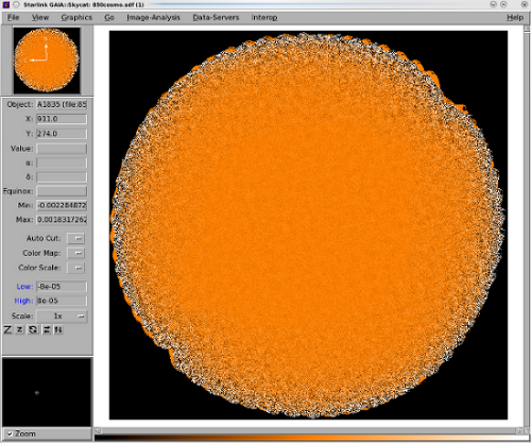
\includegraphics[width=0.48\linewidth]{sc21_850cosmo_bf}
\hspace{2mm}
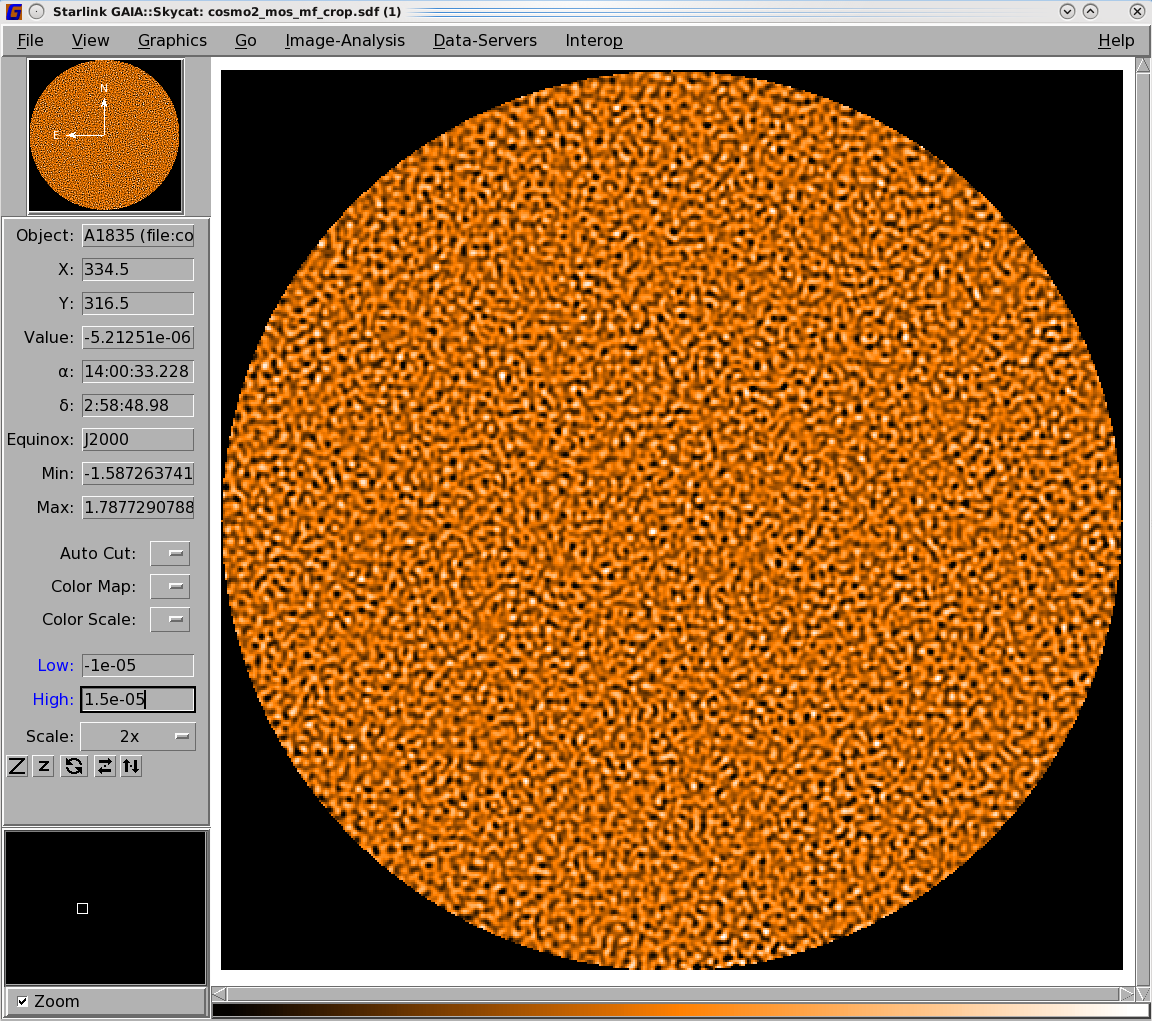
\includegraphics[width=0.48\linewidth]{sc21_850cosmo_mf_crop}
\caption[Cosmology field with the matched filter applied]{
  Reduced \textsc{pong} maps of cosmology field A1835. \textbf{Left:}
  Map reduced with \file{dimmconfig\_blank\_field.lis}.
  \textbf{Right:} Map on the left after the matched filter has been
  applied and it has been cropped.\label{fig:cosmomap}
}
\end{figure}

\textbf{Step 3: Apply the matched filter}\\
In order to optimally find sources that are the size of the telescope
beam, we apply the matched filter recipe, namely
\xref{\drrecipe{SCUBA2\_MATCHED\_FILTER}}{sun265}{SCUBA2_MATCHED_FILTER}.
We create a simple parameter file called \file{smooth.ini}:

\begin{terminalv}
[SCUBA2_MATCHED_FILTER]
SMOOTH_FWHM = 15
\end{terminalv}
where \param{SMOOTH\_FWHM~=~15} indicates that the background should be
estimated by first smoothing the map and PSF with a 15-arcsec FWHM
Gaussian. Next, the recipe is executed as follows:
%
\begin{terminalv}
% picard -recpars smooth.ini SCUBA2_MATCHED_FILTER cosmo2_mos.sdf
\end{terminalv}
%
The output of this operation is a smoothed image called
\file{cosmo3\_mos\_mf.sdf} and a cropped version is shown in the
right-hand panel of \cref{Figure}{fig:cosmomap}{figure above}. You can immediately
see the contrast to the left-hand panel which is the output from the
map-maker. A number of signal peaks now emerge as possible sources.
\\ \\
\textbf{Step 4: Crop the map}\\
Next we shall crop the map to remove the noisy edges,
in this case to a 900-arcsec radius circle. The output file will be named
\file{cosmo2\_mos\_mf\_crop.sdf}.
\begin{terminalv}
% picard CROP_JCMT_IMAGES cosmo3_mos_mf.sdf

\end{terminalv}

\starfig{sc21_850cosmo_mf_crop_snr}{}{width=0.6\linewidth}{fig:snrmask}{
  S/N map of a cosmology field}{
  Signal-to-noise map made using the \Kappa\ command \makesnr.
  The map has been scaled from 0 to $+$3.
}

\textbf{Step 5: Make an S/N map}\\
Finally, we need to find sources. The filtered map contains a
VARIANCE component, so it is easy to produce a S/N map using the
\textsc{Kappa} task \makesnr:
\begin{terminalv}
% makesnr cosmo2_mos_mf_crop cosmo2_mos_mf_crop_snr
\end{terminalv}

The resulting map, \file{cosmo2\_mos\_mf\_snr}, is shown in
\cref{Figure}{fig:snrmask}{the signal-to-noise image}. Compared with the
matched filter map the
edges no longer appear as noisy because they have been down-weighted
by the larger noise values where there were less data.
\\ \\
\textbf{Step 6: Identify sources}\\
The basic procedure for identifying sources would be to locate peaks
above some threshold S/N. The S/N image above shows peaks that are
likely to be real sources. For a start, a source appears where
expected at the 0,0 position.

But how can we check if these sources are real?
\begin{itemize}

\item One option is to split your data into mutually exclusive subsets
  and produce independent maps. Are the highest S/N peaks detected in each of
  them?
\item A second test is to compare the number of \emph{negative} peaks above
  a given S/N with the number of \emph{positive} peaks.
\end{itemize}

\subsection{Example 2 -- Advanced pipeline method}
\label{sec:jk}

Although this method is considerably simpler to execute, the products
have undergone more advanced processing than the manual method just
given. The pipeline is particularly recommended for this recipe due to
its extra analysis steps.

\textbf{Step 1: Create input file}\\
Create an file with the names of all the files you wish to process (e.g.
\file{myfiles.lis})
\\ \\
\textbf{Step 2: Run the pipeline}\\
The pipeline must first be initiated for the wavelength you are
working on. In the case below this is 850\,$\mu$m. Note that the date
does not \emph{have} to be specified when initialising the pipeline.
The pipeline is run using the
\xref{\drrecipe{REDUCE\_SCAN\_FAINT\_POINT\_SOURCES\_JACKKNIFE}}{sun264}{REDUCE_SCAN_FAINT_POINT_SOURCES_JACKKNIFE}
recipe; this uses \file{dimmconfig\_blank\_field.lis} as the
configuration file. If you wish to provide an alternative file you
will need to put the name of the new configuration file in a recipe
parameter file.  See \cref{Section}{sec:pipe}{The SCUBA-2 Pipeline}
for details.
\begin{terminalv}
% oracdr_scuba2_850 -cwd YYYYMMDD
% oracdr -loop file -files myfiles.lis -nodisplay \
-log sf FAINT_POINT_SOURCES_JACKKNIFE
\end{terminalv}

You substitute the required date for \texttt{YYYYMMDD}.
The pipeline will write out a large number of files with the following
suffices.

\begin{aligndesc}
\item[\file{sYYYYMMDD*\_fmos}]
The map for each observation

\item[\file{sYYYYMMDD*\_mappsf}] The map for each observation with an
  artificial point source added at the map centre

\item[\file{gsYYYYMMD*\_wmos}] The co-add of all the \file{\_fmos}
  files

\item[\file{gsYYYYMMD*\_whiten}] The whitened version of \file{\_wmos}

\item[\file{gsYYYYMMD*\_cal}] The calibrated version of
  \file{\_whiten}

\item[\file{gsYYYYMMD*\_mf}] The matched-filtered version of
  \file{\_cal}
\end{aligndesc}

\drrecipe{FAINT\_POINT\_SOURCES\_JACKKNIFE} is a recipe designed to
process blank field/extra-galactic data. The recipe uses a
\htmladdnormallink{jack-knife}{http://en.wikipedia.org/wiki/Jackknife_resampling}
method to remove low-spatial frequency noise and generate a matched
filter output map.

The recipe processes each observation twice, a standard reduction
first, then a re-run with a fake point source added to the time
series. This produces a co-added signal map (\file{\_wmos}) and a
coadded PSF map (\file{\_mappsf}).

\begin{tip}
The recipe name \drrecipe{FAINT\_POINT\_SOURCES\_JACKKNIFE} can be used
interchangably with  \drrecipe{REDUCE\_SCAN\_FAINT\_POINT\_SOURCES\_JACKKNIFE}.
\end{tip}


After the map-maker has completed, the recipe will call
\xref{\drrecipe{SCUBA2\_JACKKNIFE}}{sun265}{SCUBA2_JACKKNIFE}. This
routine divides the observations into two groups (odd and even) which
are co-added and then subtracted to create a jack-knife map. This map
contains only noise with no contribution from astronomical signal. The
angular power spectrum of this map is then used to estimate and remove
the residual 1/\emph{f} noise from the signal map and the PSF map;
this is the whitening step. The whitened jack-knife map is run through
\xref{\drrecipe{SCUBA2\_MATCHED\_FILTER}}{sun265}{SCUBA2_MATCHED_FILTER}
using the whitened PSF map as the PSF input. It is this matched filter
map which will be of most interest to users.

See \pipelinesun\ for more information on
\drrecipe{REDUCE\_SCAN\_FAINT\_POINT\_SOURCES\_JACKKNIFE} and all other pipeline
recipes.
\\ \\
\textbf{Step 3: (Optional) Re-run \drrecipe{SCUBA2\_JACKKNIFE}}\\
You may wish to run the \drrecipe{SCUBA2\_JACKKNIFE} step again
independently from the pipeline. If your final map does not look as
expected you might first examine the individual mosaics from the
pipeline (\file{\_fmos}), one of these observations might show visible
artefacts that you wish to exclude from the co-add. The size of the
region in the jack-knife image which is used to do the whitening step
is determined automatically, but the method may fail if the box is too
small.

If you decide to re-run this step you first co-add all the
\file{\_mappsf} files to create a coadded PSF using the \picard\ recipe
\xref{\drrecipe{MOSAIC\_JCMT\_IMAGES}}{sun265}{MOSAIC_JCMT_IMAGES}.
\begin{terminalv}
% picard MOSAIC_JCMT_IMAGES *_mappsf
\end{terminalv}
Next create a parameter file (\file{recpars.lis}) for the jack-knife
recipe (\drrecipe{SCUBA2\_JACKKNIFE}) containing the following lines.
\begin{terminalv}
[SCUBA2_JACKKNIFE]
PSF_MATCHFILTER = <name_of_above_coadded_PSF>.sdf
\end{terminalv}
Another option for this parameter file is \param{WHITEN\_BOX} to set the
size of the region used to calculate the angular power spectrum.
Finally run \drrecipe{SCUBA2\_JACKKNIFE}.
\begin{terminalv}
% picard -log sf -nodisplay -recpars recpars.lis SCUBA2_JACKKNIFE *fmos.sdf
\end{terminalv}
This will create files beginning with \file{pgYYYMMDD}$\ldots$ that
should have the same suffices as above: \file{\_wmos},
\file{\_whiten}, \file{\_cal}, and \file{\_mf}.



\section{\xlabel{Galactic}Extended galactic sources}
\label{sec:bright_ex}

This example is concerned with recovering bright extended emission.
The signal from extended emission varies slowly as seen by the array
passing over it. It thus appears at lower frequencies in the power
spectrum and complicates the high-pass filter selection. Too harsh a
filter will make flat maps but any extended emission will have been
removed in doing so.
\\ \\
\textbf{Step 1: Running the map-maker}
\vspace{0.2cm}\\
We run the map-maker using \file{dimmconfig\_bright\_extended.lis};
we have also specified a couple of overrides on the command
line---\xparam{MAPTOL}{maptol}~=~0.04 is slightly more stringent than default and
\xparam{AST.ZERO_SNR}{ast.zero\_snr}~=~3.5 constrains emission everything below
3.5\,$\sigma$ to zero.

In this example we give the map-maker a file containing a list of the
input files (\file{filelist.txt}) and
\file{dimmconfig\_bright\_extended.lis} is in the local directory.

\begin{terminalv}
% makemap in=^filelist.txt 850galactic \
          config='"^dimmconfig_bright_extended.lis,maptol=0.04,ast.zero_snr=3.5"'
\end{terminalv}
The resulting map is shown in \cref{Figure}{fig:galmakemap}{the figure below}.

\starfig{sc21_gal_11}{[t!]}{width=0.6\linewidth}{fig:galmakemap}{
  Galactic example: initial reduction using \file{dimmconfig\_bright\_extended.lis}}{
  The output from the map-maker using \file{dimmconfig\_bright\_extended.lis}.
}

\textbf{Step 2: Generating an external mask}
\vspace{0.2cm}\\
Next we create an external mask from the output of \makemap. Here we
follow the steps outlined in \cref{Section}{sec:mask}{Masking options}.

\begin{terminalv}
% makesnr 850map 850map_snr
\end{terminalv}

This S/N map is thresholded to set everything below 3\,$\sigma$ to 0 and
everything above to 1.

\begin{terminalv}
% thresh 850map_snr 850map_mask thrlo=3 newlo=0 thrhi=3 newhi=1
\end{terminalv}
The thresholded map is shown in the left-hand panel of
\cref{Figure}{fig:mask}{this figure}. The next step is to smooth this map
by convolving it with a Gaussian of 16\,arcsec. For this we use a factor
of 4 for the FWHM parameter.

\begin{terminalv}
% gausmooth 850map_mask 850map_mask_sm fwhm=4
\end{terminalv}

We threshold the map again to produce our mask. In this case all
values below out threshold are set to `bad'. The the smoothed map now
has values scaled between 0 and 1, we set our threshold at 0.02 to
include more of the emission beyond the 3\,$\sigma$ edge.
\begin{terminalv}
% thresh 850map_mask_sm 850map_mask_zm thrlo=0.02 newlo=bad thrhi=0.02 newhi=1
\end{terminalv}
The final mask is shown in the right-panel of \cref{Figure}{fig:mask}{the figure below}.
Note how it encompasses more emission and has softer edges than the
first threshold map. \\

\begin{figure}[t]
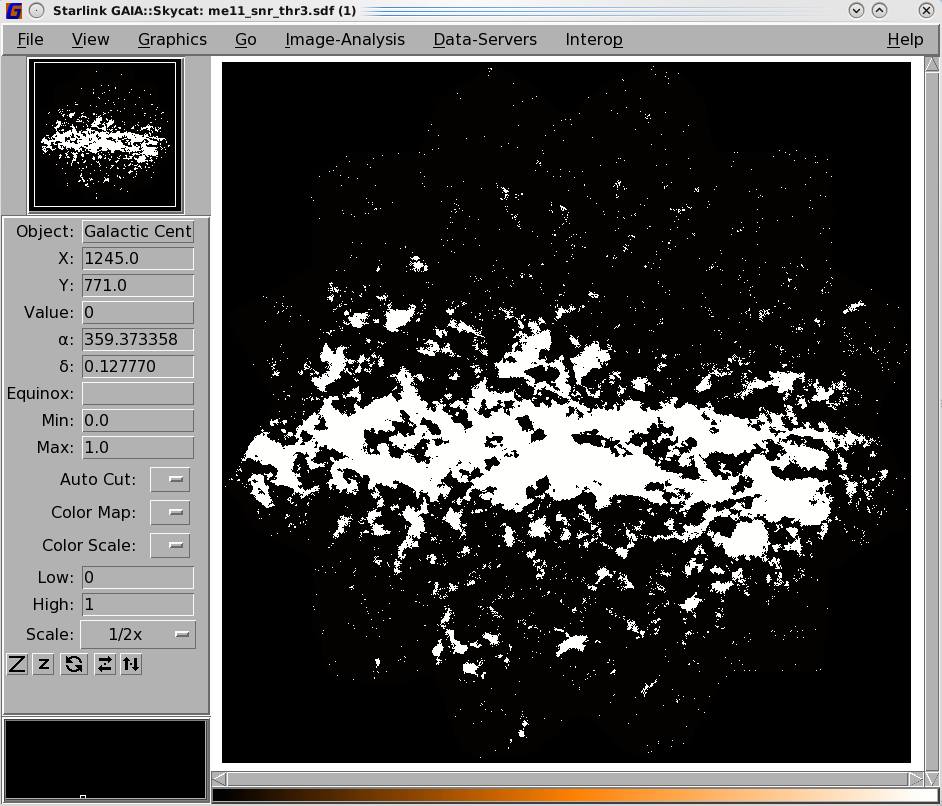
\includegraphics[width=0.475\linewidth]{sc21_gal_mask1}
\hspace{2mm}
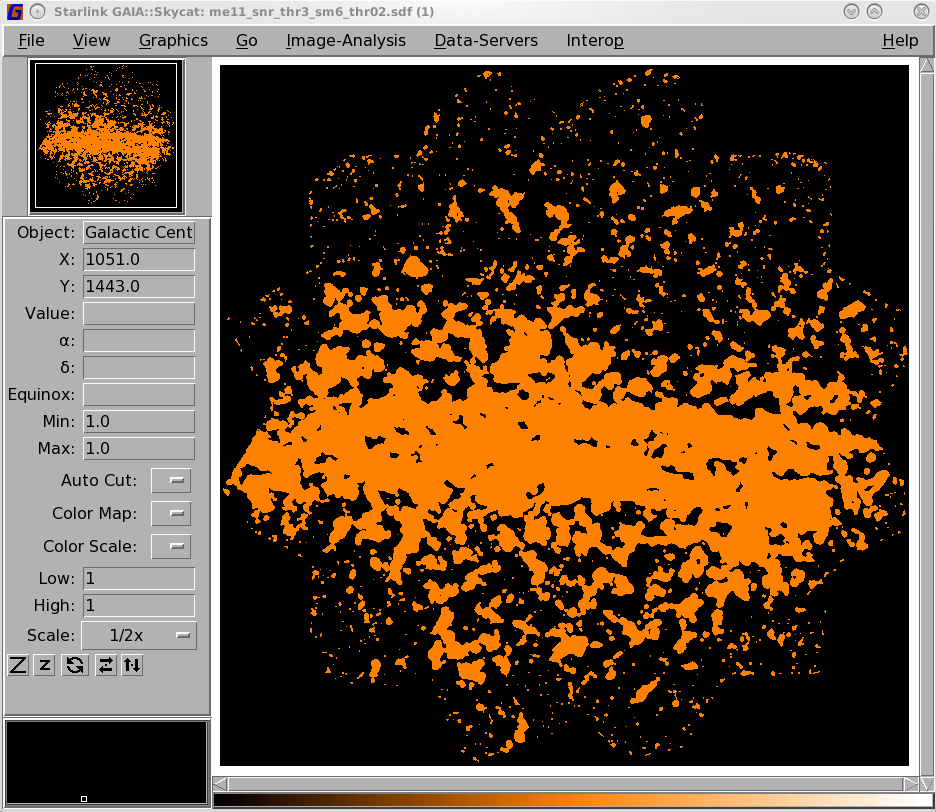
\includegraphics[width=0.475\linewidth]{sc21_gal_mask2}
\caption[Galactic example: thresholded SNR map and smoothed map]{
  \textbf{(Left)} The initial mask created by thresholding 850map\_snr
  to 3$\sigma$. \textbf{(Right)} Second mask made by thresholding the
  smoothed map to 0.02.\label{fig:mask}
}
\end{figure}


\textbf{Step 3: Re-running the map-maker with an external mask supplied}
\vspace{0.2cm}\\
As a last step the map is re-made with this mask supplied as an external
file. For this run we apply the additional parameters in a
personalised configuration file, \file{mydimmconfig.lis}.
\begin{terminalv}
% makemap in=^filelist.txt 850galactic \
          config=^mydimmconfig.lis ref=850map_mask_zm
\end{terminalv}

The configuration file, \file{mydimmconfig.lis}, has the following
format---note how it is based on
\file{dimmconfig\_bright\_extended.lis}. It has decreased the
convergence parameter to \xparam{MAPTOL}{maptol}~=~0.03 but increased the number
of iterations to compensate as 40 is unlikely to be sufficient.
\begin{terminalv}
^$STARLINK_DIR/share/smurf/dimmconfig_bright_extended.lis
numiter = -100
noisecliphigh = 10.0
maptol = 0.03
ast.zero_mask=1
ast.zero_snr = 0
\end{terminalv}

\textbf{Step 4: Cropping the map}
\vspace{0.2cm}\\
We now crop the map to remove the noisy edges using the \picard\ recipe
\drrecipe{CROP\_JCMT\_IMAGES}. To determine what to trim we can look
at the exposure-time image with \gaia.  See
\cref{Figure}{fig:exptime}{the exposure time image}.

\starfig{sc21_gal_exptime}{[h!]}{width=0.7\linewidth}{fig:exptime}{
  Galactic example: exposure time map}{
  The exposure-time image of the science map from \cref{Figure}{fig:galmakemap}{
  our example map}. You can right-click and drag the mouse
  between two points to measure the distance. Here we see the exposure
  time dropping off sharply at a radius of 30\,arcmin. A non-default
  colour scale has been chosen to illustrate the morphology.
}

The exposure-time map shows a sharp drop off at a radius of 30\,arcmin.
We can thus specify a parameter file like below.
\begin{center}
\begin{terminalv}
[CROP_JCMT_IMAGES]
MAP_RADIUS = 1800
\end{terminalv}
\end{center}

\begin{terminalv}
% picard CROP_JCMT_IMAGES 850galactic.sdf
\end{terminalv}
The final cropped map is shown in \cref{Figure}{fig:crop_map}{this plot}.
Compared with the first map out of the map-maker
(\cref{Figure}{fig:galmakemap}{first map}),
slightly more of the faint extended emission is apparent.

One of the challenges facing this type of reduction is the need to
account for both faint extended structure and very bright sources in
the same map. You may find some degree of bowling remains around the
brightest sources.

There are areas you may wish to experiment with. One is to adjust the
filtering. Another option is to supply an external mask from
a different dataset, e.g. a
\htmladdnormallink{Herschel}{http://herschel.esac.esa.int/} map.
See \cref{Chapter}{sec:tweak}{Tailoring Your Reduction} for further
discussion.

\starfig{sc21_gal12_crop}{[b!]}{width=0.65\hsize}{fig:crop_map}{
  Galactic example: cropped final map}{
  The final cropped, reduced map from the map-maker run with
  an external mask supplied.
}


\clearpage

\newpage
\chapter{\xlabel{postprocess}Post-processing Reduction Steps}
\label{sec:postprocess}

\section{\xlabel{apply_fcf}Flux conversion factors}
\label{sec:cmult}

When your data comes out of the map-maker it is in units of picowatts
(pW). A flux conversion factor, or FCF, needs to be applied to scale
your data from units of pW to janskys (Jy). For more information on
calibrating SCUBA-2 data see Dempsey et al. (2013) \cite{dempsey12}.


Below are our default FCFs.
\vspace{0.5cm}
\renewcommand*\arraystretch{1.2}

\begin{table}[h!]
\centering
\begin{tabular}{|c|c|c|c|}
\hline
\multicolumn{2}{|c|}{\textbf{APERTURE}}  &
\multicolumn{2}{c|}{\textbf{PEAK}}      \\
\hline
\multicolumn{2}{|c|}{\fcfa\ (Jy/pW/arcsec$^2$) }  &
\multicolumn{2}{c|}{\fcfb\ (Jy/pW/beam)}      \\
\hline
\hspace{0.4cm} 450\,$\mu$m \hspace{0.3cm} & 850\,$\mu$m & \hspace{0.4cm} 450\,$\mu$m \hspace{0.3cm}& 850\,$\mu$m \\
\hline
4.71 $\pm$ 0.5& 2.34 $\pm$ 0.08& 491 $\pm$ 67& 537 $\pm$ 24 \\
\hline
\end{tabular}
\end{table}
\renewcommand*\arraystretch{1.0}
\vspace{0.5cm}

\begin{sltextbox}{IMPORTANT NOTES:}
  \begin{itemize}
  \item The standard FCF to be applied depends on the reduction date
    for your data. For data that have been \emph{reduced prior} to
    July 2012 you should see \cref{Appendix}{app:fcfs}{FCFs by
      reduction date} for alternative FCFs.

  \item Due to a glitch in the WVM, data reduced between 2012
    September 19, and 2013 January 18 must be re-reduced using a
    recent version of Starlink (Hikianalia or later), or should have
    an FCF derived from a calibrator reduced at the same time (and not
    our standard FCF) applied to it.
  \end{itemize}
\end{sltextbox}


\subsection{Aperture flux}

To get the flux density of extended sources with aperture photometry
you should apply the \fcfa.  You can then sum the emission in an
aperture. \fcfa\ was determined using a 60-arcsec diameter
aperture. If your aperture differs from this you should scale your
flux accordingly---the scaling factor can be read off the curve of
growth (see \cref{Appendix}{app:cog}{this appendix}). This graph gives
the ratio of aperture flux to total flux for a range of aperture
diameters.

\fcfa\ is determined using 1-arcsec pixels. For different pixel sizes
you will also need to multiply by the pixelsize squared.

\subsection{Peak flux}

If you want to read off the peak flux from your map, you should apply
the \fcfb\ (also known as the peak FCF).  When you open your map in
\gaia\ the value of the brightest pixel will be the peak flux of your
source. (If your source is point-like, the peak value in the map is
the total flux density). Applying \fcfb\ will result in a map with
units of Jy/beam. For point-like or compact sources smaller than the
beam (with a Gaussian profile), this peak value will be the flux
density of your source.

\subsection{\xlabel{own_fcf}Determining your own Flux conversion factors}
\label{sec:own_fcf}

Calibration observations are taken at various points throughout the
night and we recommend you compare the FCF calculated from your
nearest calibrator to the standard FCF. You can use this FCF to scale
the the standard value accordingly. You should chose the calibrator
nearest in time to your science observations, unless the weather has
changed significantly.

\begin{enumerate}
\item Reduce the calibrator with the map-maker using
  \file{dimmconfig\_bright\_compact.lis} as the configuration file.

\item Determine the FCF value by passing the output map to the
  \picard\ recipe
  \xref{\drrecipe{SCUBA2\_CHECK\_CAL}}{sun265}{SCUBA2_CHECK_CAL}.

\begin{terminalv}
% picard SCUBA2_CHECK_CAL 850calibrator.sdf
\end{terminalv}

This will produce a log file (\file{log.checkcal}) which records the
both \fcfb\ and \fcfa. Check that these values closely approximate the
standard FCF values given above.

\item Re-reduce the calibrator using the map-maker with the
  \emph{same} configuration file you used for your science
  observations.

\item Again determine the FCF using \drrecipe{SCUBA2\_CHECK\_CAL}.

\item Apply this FCF to your reduced science data using \cmult---see
  the next section. Remember to apply the pixel size squared factor if
  using \fcfa.
\end{enumerate}

\subsection{Applying the FCF}
\label{subsec:ApplyingFCF}

You can apply the FCF using the \picard\ recipe
\xref{\drrecipe{CALIBRATE\_SCUBA2\_DATA}}{sun265}{CALIBRATE\_SCUBA2\_DATA}.
By default this will multiply your map by 1000$\times$\fcfb, obtained
from the start of \cref{Section}{sec:cmult}{Flux conversion
  factors}. This produces a calibrated map with units of mJy/beam.

You can supply a parameter file if you wish to use a different value
for the FCF or use \fcfa. The recipe will write out the calibrated
file with an \file{\_cal} suffix and will change the units in the map
header.

\begin{terminalv}
% picard CALIBRATE_SCUBA2_DATA  mapinpW.sdf
\end{terminalv}

Note that the recipe will also take account of the pixel size when
applying \fcfa.

\section{\xlabel{crop}Cropping your map}
\label{sec:crop}

The nature of the scan patterns results in SCUBA-2 maps significantly
larger than the requested size. The high noise towards the outer edges
is a consequence of the scanning pattern. Although this excess data
are down-weighted during reduction by the map-maker, you may wish to
remove it before either combining maps (see
\cref{Section}{sec:coadd}{Co-adding multiple maps}) or publishing your
map.

You can crop your map to the map-size set in the data header or to any
requested size of box or circle using the \picard\ recipe
\xref{\drrecipe{CROP\_SCUBA2\_IMAGES}}{sun265}{CROP\_SCUBA2\_IMAGES}.
The centre of the cropping area will always be the centre of your map.

\begin{terminalv}
% picard -recpars mypar.lis CROP_SCUBA2_IMAGES map_cal.sdf
\end{terminalv}

The example above includes a parameter file specifying the radius of
the circle to be extracted (in arcsecs).  The format for the parameter
file is shown below.

\begin{terminalv}
[CROP_SCUBA2_IMAGES]
MAP_RADIUS = 1800.0
CROP_METHOD = circle
\end{terminalv}


If this parameter file is omitted it will default to a box of sides
equal to the map size in the header (as requested in the MSB). The
output from \drrecipe{CROP\_SCUBA2\_IMAGES} is a file with the suffix
\file{\_crop}. Full details of this recipe can be found in the
\htmladdnormallinkfoot{\textsc{Picard}
  website}{http://www.oracdr.org/oracdr/PICARD}

\begin{tip}
  The default crop shape will be a square. Avoid losing good data by
  specifying a circle using the parameter file.
\end{tip}

\section{\xlabel{coadd}Co-adding multiple maps}
\label{sec:coadd}

You may have multiple maps of the same source which you would like to
co-add. \picard\ has a recipe called
\xref{\drrecipe{MOSAIC\_JCMT\_IMAGES}}{sun265}{MOSAIC_JCMT_IMAGES}
that co-adds maps while correctly dealing with the exposure time and
weights NDF extensions. The images are combined using inverse-variance
weighting and the output variance is derived from the input variances.

\begin{terminalv}
% picard -recpars mypar.lis MOSAIC_JCMT_IMAGES 850map*_cal_crop.sdf
\end{terminalv}

This creates a single output file based on the name of the last file
in the list, and with a suffix \file{\_mos}.

There are a number of options associated with
\drrecipe{MOSAIC\_JCMT\_IMAGES} (see the \textsc{Picard} manual for a full
description). However, the main one is choosing between \wcsmosaic\
(default) and the \ccdpack\ option \makemos\ for the combination
method. For more information on \task{makemos} and advice on choosing the
best method see \xref{\textbf{SUN/139}}{sun139}{}.

The example parameter file below chooses \task{makemos} using a 3-$\sigma$
clipping threshold.

\begin{terminalv}
[MOSAIC_JCMT_IMAGES]
MOSAIC_TASK = makemos
MAKEMOS_METHOD = sigmas
MAKEMOS_SIGMAS = 3
\end{terminalv}

Currently there is no advantage in terms of data quality to reducing
all observations simultaneously or separately. However, the latter
does allow the option of assessing the individual maps before co-adding.

\begin{tip}
  The list of files can be the output from \texttt{cat}. Remember
  to include the back quotes.  For example, \texttt{\% picard
    MOSAIC\_JCMT\_IMAGES \`{}cat myfiles.txt\`{}}.
\end{tip}


\subsection{Registering maps}

You can register a series of SCUBA-2 maps to a common reference
position using the \picard\ recipe
\xref{\drrecipe{SCUBA2\_REGISTER\_IMAGES}}{sun265}{SCUBA2\_REGISTER\_IMAGES}.
This is only possible if a there is a common, known source that is
present in \textit{all} of the input maps. This should be done before
combining your maps.

\begin{terminalv}
% picard -recpars myparams.ini SCUBA2_REGISTER_IMAGES `cat listoffiles.txt`
\end{terminalv}

Here the parameter file contains the equatorial position of the
reference source as in the example below. See \picardsun\ for more
details.

\begin{terminalv}
[SCUBA2_REGISTER_IMAGES]
REGISTER_IMAGES = 1
REGISTER_X  = HH:MM:SS.S
REGISTER_Y  = DD:MM:SS.S
\end{terminalv}

\param{REGISTER\_X} and \param{REGISTER\_Y} may also be galactic
longitude and latitude respectively, both measured in decimal
degrees.

\section{\xlabel{noise}Sensitivity}

\subsection{Getting the noise}
\label{sec:mapstats}

You can use the \picard\ recipe \drrecipe{SCUBA2\_MAPSTATS} to get the
noise. This recipe estimates the RMS from both the map, the NEP, and
the RMS predicted by the Integration Time Calculator. It then writes out
a series of results in a log file called \file{log.mapstats}. The
parameters written to this file are listed in
\cref{Appendix}{app:mapstats}{SCUBA2_MAPSTATS}.

\begin{terminalv}
% picard SCUBA2_MAPSTATS map.sdf
\end{terminalv}
This recipe will report the noise in the same input units provided. 


\textbf{Note:} \drrecipe{SCUBA2\_MAPSTATS} is only designed to work on
reductions of single observations. On coadded observations it could
produce misleading results, or even fail completely to work.

If multiple files are run through \drrecipe{SCUBA2\_MAPSTATS}, either in a single call
of PICARD or by repeatedly running PICARD in the same terminal on different
files, the results will be appended to the existing log.mapstats file.
The final columns — project, recipe and filename — are given to ensure it
is clear to users which line of the logfile corresponds to which input file.

\subsubsection*{Steps for getting your coadded-map noise}
After applying any necessary FCF, \drrecipe{SCUBA2\_MAPSTATS} simply
executes the following steps to get the map noise.

\begin{enumerate}
\item Crop the map to remove the noisy edges.

\begin{terminalv}
% picard CROP_JCMT_IMAGES map_cal.sdf
\end{terminalv}

\item Run the \Kappa\ command \stats\ to extract the median value from
the error array.

\begin{terminalv}
% stats map_cal_crop comp=err order
\end{terminalv}

\end{enumerate}

\begin{tip}
  Use the error array to avoid contamination of the noise distribution
  from bright sources.
\end{tip}


\subsection{Map statistics}

The \Kappa\ commands \histat\ and \stats\ are very similar and both
return a range of statistics describing any NDF. In addition to the
main data array they can be passed the error (\param{comp=err}), variance
(\param{comp=var}) or quality (\param{comp=qua}) arrays (if available).

The reported statistics include the pixel maximum and minimum,
standard deviation, number of pixels used and omitted, along with
pixel mode, and mean.  If you supply the \xparam{ORDER}{order} keyword,
the median is also shown.

\begin{terminalv}
% stats comp=err map_cal_crop order
\end{terminalv}

\textbf{Note:} the standard deviation of the data array will give a
similar result to the mean/median of the error array except with
additional contamination from sources.



\subsection{Viewing the noise histogram}

You can view a histogram of the error array with the
\textsc{Kappa} command \histogram. Again \param{comp=err} must be
specified.

\begin{terminalv}
% histogram map_cal_crop comp=err numbin=200 style="color=white"
\end{terminalv}
The output is shown in the \cref{Figure}{fig:noihisto}{the plot below}.
For more information on the options for \histogram\ see
\kappasun.

\starfig{sc21_noihist}{}{width=0.7\linewidth}{fig:noihisto}{
  The error array viewed with \textsc{Kappa} command \task{histogram}.}{
  The error array viewed with \textsc{Kappa} command \task{histogram}.
}

\subsection{Examining the error map with GAIA}

It is also useful to view the error map itself. Open your reduced map
in \gaia, then select the \gaiathing{Error} button on the
\gaiathing{Select NDF in container file} window---see
\cref{Figure}{fig:noigaia}{the figure below}. You will need to adjust
the scaling to view the error map properly.

To assess the noise using \gaia, go to the toolbar on the main window
and click on \gaiathing{Image-Analysis$\Rightarrow$Image
regions}. Next select the region shape you would like to check and
draw it on your map by clicking and dragging the mouse. Click the
\gaiathing{Stats selected} button in the \gaiathing{Image regions}
window to get a report of the statistics in the selected region.

\begin{tip}
  You can write out the error array of your map into a new NDF using
  the \textsc{Kappa} command \ndfcopy. For example, \texttt{\% ndfcopy
    map comp=err map\_err}
\end{tip}



\starfig{sc21_noigaia6}{[h!]}{width=\linewidth}{fig:noigaia}{
  The error map viewed with \gaia}{
  The error array displayed with \gaia. After clicking the
  \gaiathing{Error} button (circled in red) you will have to rescale your map.
}


\section{\xlabel{regridding}Regridding your data}
\label{sec:regriddata}

To change the pixel size use the \Kappa\ command \compave. The
following example increases the pixel size from 4\,arcsec to 8\,arcsec
by using a compression factor of 2.

\begin{terminalv}
% compave map map_regrid 2
\end{terminalv}

\begin{tip}
  Remember you can use \ndftrace\ if you are unsure of the pixel size.
\end{tip}


% they find that smaller pixels produce higher peak values (due to the
% smaller pixels producing less smoothing that larger pixels), and
% also converge faster (due to each pixel needing to be consistent
% with fewer bolometers). The average noise per pixel is higher for
% smaller pixels (as expected), and this means that the SNR level used
% for masking needs to be adjusted to get the same mask produced using
% larger pixels.

\section{\xlabel{maskshow}Displaying masks}
\label{sec:maskshow}

SCUBA-2 maps created using ``\model{AST}-masking'' (see \cref{Section}
{sec:masking}{Masking}) will contain a \texttt{Quality} array indicating the
background pixels that were masked (i.e. forced to zero). In itself this
is fairly simple - background pixels have a non-zero Quality value and
source pixels have a Quality value of zero. However, it is also possible
to have independent masks for the \model{FLT} and \model{COM} models,
in addition to the \model{AST} mask. For instance, maps created using
\brightextended\ or \jsageneric\ will have \texttt{Quality} arrays that
contain both a \model{FLT} and an \model{AST} mask, and so some care needs
to be used when interpreting the \texttt{Quality} array.

Each value in the \texttt{Quality} array is restricted to taking integer values
between 0 and 255, and so can be thought of as 8 separate bits. Each ``bit
plane'' within the \texttt{Quality} array holds a single mask - \model{AST},
\model{FLT} or \model{COM}. The \xref{\task{showqual}}{sun95}{SHOWQUAL}
command can be used to find out which mask is held by which bit plane:

\begin{terminalv}
% showqual fred.sdf
   AST (bit 1) - "Set iff AST model is zeroed at the output pixel"
   FLT (bit 2) - "Set iff FLT model is blanked at the output pixel"
\end{terminalv}

This means that the \model{AST} mask is stored in bit 1 (the least significant
bit), the \model{FLT} mask is stored in bit 2, and there is no \model{COM}
mask. Note, if
a map was produced using \model{FLT} masking but no \model{AST} masking,
then the \model{FLT} mask would be stored in bit 1.

The decimal integer value of any element of the \texttt{Quality} array is
equal to the binary value formed from the bits listed by \task{showqual}.
So in the above case the maximum \texttt{Quality} value is 3 (the decimal
equivalent of binary ``11'' --- both bits set). Remembering that a bit is set
(\emph{i.e.} is 1) for background pixels and cleared (\emph{i.e.} is 0) for
source pixels, it follows that the four possible decimal \texttt{Quality}
values in the above case (0-3) are:

\begin{enumerate}
\item - neither bit set, so the pixel is inside both the \model{AST} and the \model{FLT} mask
(a source pixel).

\item - bit 1 set but not bit 2, so the pixel is outside the \model{AST} mask but
inside the \model{FLT} mask (a border-line pixel).

\item - bit 2 set but not bit 1, so the pixel is inside the \model{AST} mask but
outside the \model{FLT} mask (a border-line pixel).

\item - both bits set, so the pixel is inside neither mask (a background
pixel).
\end{enumerate}

\cref{Figure}{fig:qualmap}{Quality component displayed as an image} shows
a simple map of the \texttt{Quality} array values --- the black areas have
value zero and are thus inside both masks, the dark brown areas have value 2
and are thus inside the \model{AST} mask but outside the \model{FLT} mask.
The light brown areas have value 3 and are inside neither mask. In this
particular case, there are no  areas with a quality value of 1, so the
\model{FLT} mask is contained entirely within the \model{AST} mask.

\begin{figure}[t!]
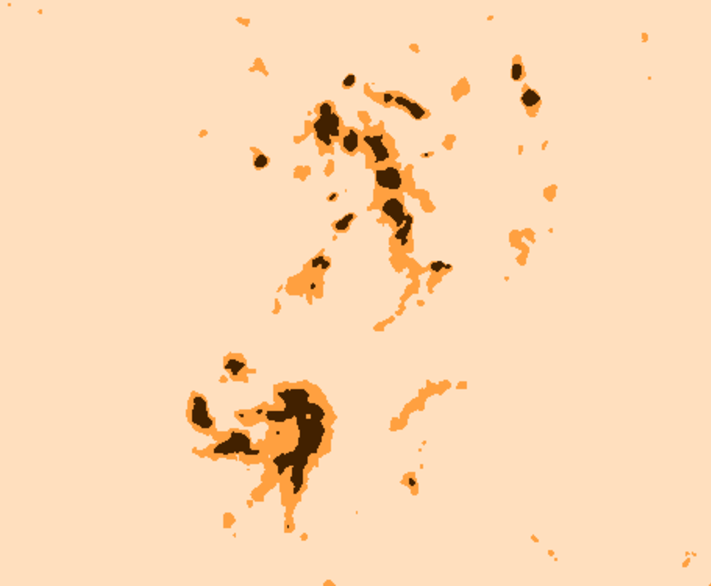
\includegraphics[width=0.6\linewidth]{sc21_qual}
\caption[Quality component displayed as an image]{The quality component
from a typical map.}
\label{fig:qualmap}
\end{figure}

To produce a plot like this, first open your map in \textsc{Gaia}. Select
the top level NDF from list in the pop-up window then click the
\gaiathing{Quality} button. You will need to rescale the map to bring
out the masks--see \cref{Figure}{fig:qualdisp}{} for another example
showing the full \textsc{Gaia} window (using rather brighter colours this
time!).

\starfig{sc21_qualitygaia}{[t!]}{width=0.9\hsize}{fig:qualdisp}{
   Display of the mask made by the map-maker}{
   Using \gaia\ to display the mask applied by the map-maker. Select the
   QUALITY component of your map.
}

There are several commands within \textsc{Kappa} that manipulate
\texttt{Quality} arrays in various ways. For instance, the
\xref{\task{setbb}}{sun95}{SETBB} command allows pixel data values to
be set bad if the associated \texttt{Quality} value has a specified
collection of set bits. Thus:

\begin{terminalv}
% setbb fred 1
\end{terminalv}

will set all pixels bad in \texttt{fred.sdf} except for those inside the
\model{AST} mask. Likewise,

\begin{terminalv}
% setbb fred 2
\end{terminalv}

will set all pixels bad except for those inside the \model{FLT} mask.  Note, the
change made by \task{setbb} is temporary - it can be undone by doing:

\begin{terminalv}
% setbb fred 0
\end{terminalv}

To display the \texttt{fred.sdf} map and then overlay the \model{AST} mask in blue
and the \model{FLT} mask in red, do:

\begin{terminalv}
% gdclear
% display fred mode=perc percentiles=\[2,98\]
% setbb fred 1
% contour fred clear=no mode=good labpos=! style='colour=blue'
% setbb fred 2
% contour fred clear=no mode=good labpos=! style='colour=red'
% setbb fred 0
\end{terminalv}

The resulting plot is shown in \cref{Figure}{fig:masks}{AST and FLT masks
shown together}.

\begin{figure}[t!]
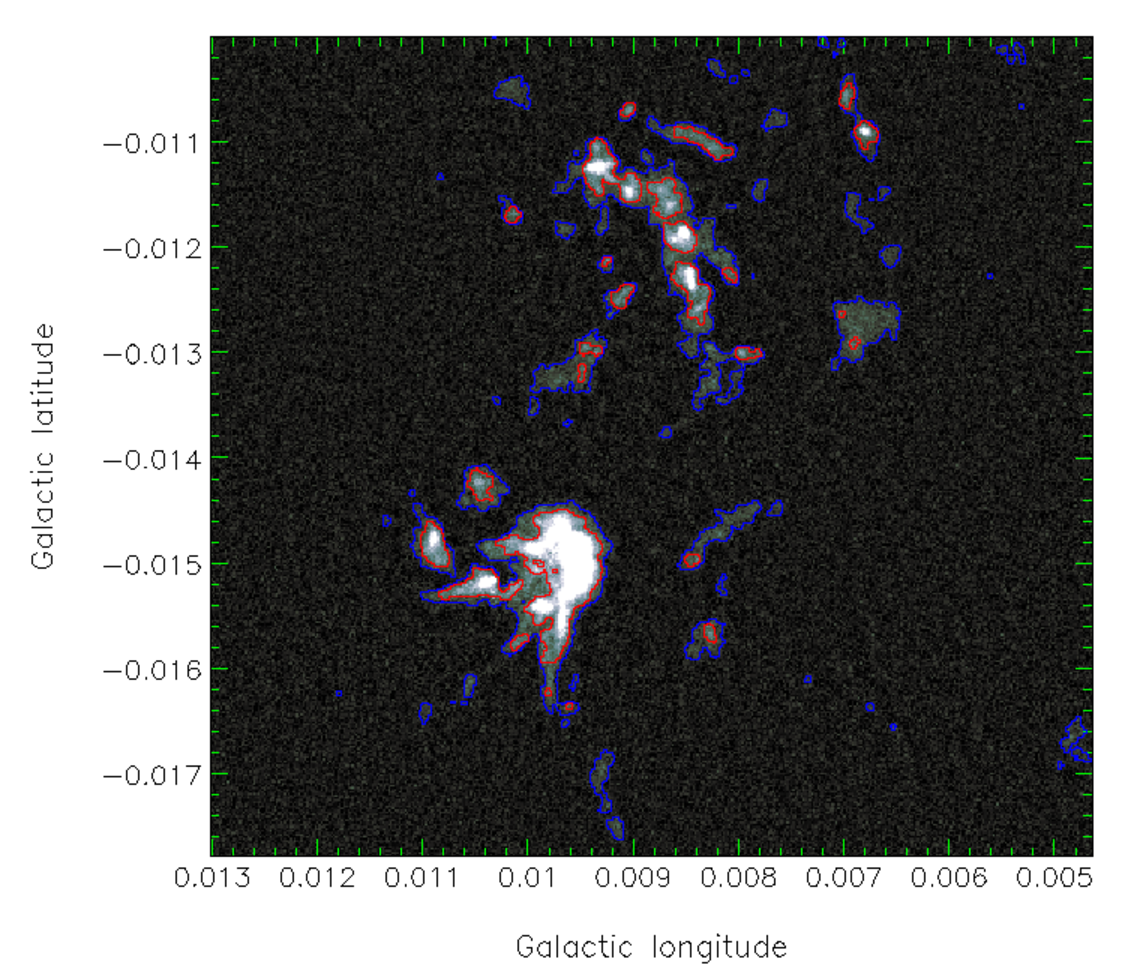
\includegraphics[width=0.6\linewidth]{sc21_masks}
\caption[AST and FLT masks shown together]{The AST and FLT masks contoured
together over an image.}
\label{fig:masks}
\end{figure}

Alternatively, \gaia\ can be used to contour the \texttt{Quality} array
over an image, but you cannot then distinguish the \model{AST} mask from
the \model{FLT} mask. First you will need to copy out the QUALITY component
of the data to a separate file using \task{ndfcopy}:

\begin{terminalv}
% ndfcopy comp=qua map map_mask
\end{terminalv}

Then open your map in \gaia\ and contour the mask NDF on top.
Select \gaiathing{Contouring...} from the \gaiathing{Image-Analysis}
menu, and supply the name of the mask NDF either by entering its name in
the \gaiathing{Other image:} box, or selecting with
\gaiathing{Choose file...} file browser. See
\cref{Figure}{fig:maskdisp}{the figure below}.

For more information on the use of masks by \makemap\ and the
parameters that affect them see \cref{sectyion}{sec:masking}{Masking}.

\starfig{sc21_dispmask3}{[hb!]}{width=0.95\linewidth}{fig:maskdisp}{
   Contours of an \model{AST} mask overlaid on a map}{
   Using \gaia\ to display your map with the \model{AST} mask used by
   the map-maker contoured on top.
}


\section{\xlabel{match_filter}Point-source extraction: the matched filter}
\label{sec:mf}

This effectively fits a single Gaussian point spread function (PSF),
centered over every pixel in the map, and applies a background
suppression filter to remove any residual large-scale noise.

Cosmology maps usually contain very faint sources that often need
extra help extracting. The \picard\ recipe
\xref{\drrecipe{SCUBA2\_MATCHED\_FILTER}}{sun265}{SCUBA2_MATCHED_FILTER}
can be used to improve point-source detectability.

The matched filter works by smoothing the map and PSF with a broad
Gaussian, and then subtracting from the originals. The images are then
convolved with the modified PSF. The output map should be used
primarily for source detection only. Although the output is normalised
to preserve peak flux density, the accuracy of this depends on how
closely the real PSF matches the telescope beam size. In the case of
nearby sources, each ends up contributing flux to both peaks.

\begin{terminalv}
% picard -recpars mypar.lis SCUBA2_MATCHED_FILTER 850_map_cal_crop.sdf
\end{terminalv}

As in the example parameter file below we have requested the
background should be estimated by first smoothing the map and PSF with
a 15-arcsec Gaussian.

\begin{terminalv}

[SCUBA2_MATCHED_FILTER]
SMOOTH_FWHM = 15

\end{terminalv}

This is a fairly common technique used throughout the extra-galactic
sub-millimetre community to identify potential sources. A full
description of the matched filter principle is given in
\cref{Appendix}{app:mf}{SCUBA-2 matched filter}, while the
\textsc{Picard} manual gives full details of all the available
parameters.

\section{\xlabel{clumps}Clump finding}
\label{sec:clumps}
\label{sec:clumpfind}

The \cupid\ application \findclumps\ can be used to generate a clump
catalogue. It identifies clumps of emission in one-, two- or
three-dimensional NDFs. You can select from the clump-finding
algorithms ``FellWalker''\cite{fellwalker}, ``Gaussclumps'',
``ClumpFind'' or ``Reinhold'' and must supply a configuration file
specific to each method. See the \xref{\textsc{Cupid} manual}{sun255}{}
for descriptions of the various algorithms.

The result is returned as a catalogue in a text file and as a NDF
pixel mask showing the clump boundaries.

\begin{terminalv}
% findclumps in=S2map.sdf out=clumpmap.sdf outcat=clumps.FIT logfile=clumps.log \
  config=^config.dat method=fellwalker rms=25 shape=polygon
\end{terminalv}

The shape option allows \findclumps\ to create an
\htmladdnormallink{STC-S}{http://ivoa.net/documents/STC-S/index.html}
description (polygonal or elliptical) for each clump. These are added
as extra columns to the output catalogue.

\begin{aligndesc}
\item[Polygon] Each polygon will have, at most, 15 vertices. For
  two-dimensional data the polygon is a fit to the clump's outer
  boundary (the region containing all good data values). For
  three-dimensional data the spatial footprint of each clump is
  determined by rejecting the least significant 10\% of spatial
  pixels, where "significance" is measured by the number of spectral
  channels that contribute to the spatial pixel. The polygon is then a
  fit to the outer boundary of the remaining spatial pixels.

\item[Ellipse] All data values in the clump are projected onto the
  spatial plane and "size" of the collapsed clump at four different
  position angles---all separated by 45$^\circ$---is found. The
  ellipse that generates the same sizes at the four position angles is
  then found and used as the clump shape.
\end{aligndesc}

\starfig{sc21_plotstcshapes}{[ht!]}{width=1.0\linewidth}{fig:stcshapes}{
  Overlaying a clump catalogue in \gaia.}{
  STC shapes displayed over the input map with \gaia. To overlay your clumps
  in this way display your map with \textsc{Gaia}. Under the \gaiathing{Image-Analysis}
  menu select \gaiathing{Positions...} followed by \gaiathing{Import CUPID
  catalogue...} In the pop-up window select the \file{.FIT} file
  generated by \findclumps\ and ensure the \gaiathing{STC shape} box is
  checked before importing.
}


\section{\xlabel{provenance}Map provenance \& configuration parameters}
\label{sec:prov}

You may want to check a reduced file to determine which raw files went
into it and what configuration parameters were used with the
map-maker. There are a number of useful \Kappa\ commands to help you
with this:

\begin{description}
\item[Map provenance]
  \provshow\ will list all the NDFs and operations that were used in the
  creation of your map, while \hislist\ will show a truncated list of input
  files and operations but will list every configuration parameter used by
  the map-maker.  This includes all the hidden default values as well as
  those specified in your supplied configuration file. These commands are
  executed like this:

\begin{terminalv}
% provshow 850map
% hislist 850map
\end{terminalv}

The output of \task{provshow} can be very long.  If you merely want to
know what the original files were, the ones with no parents, select the
root ancestors.

\begin{terminalv}
% provshow 850map show=roots
\end{terminalv}


\item[Map-maker parameters]
The task \configmeld\ will compare two maps and highlight any differences
between the configuration parameters that were used to create the maps. A
configuration file can be supplied in place of a map, in which case the
parameters used to create the map are compared with those in the
configuration file. \task{configmeld} requires a visual-differences tool
to be installed on your machine; those currently recognised are:
\htmladdnormallink{\texttt{meld}}{http://meldmerge.org/}
\htmladdnormallink{\texttt{opendiff}}{http://developer.apple.com/},
\htmladdnormallink{\texttt{diffmerge}}{http://www.sourcegear.com/diffmerge},
\htmladdnormallink{\texttt{kdiff3}}{http://kdiff3.sourceforge.net},
\htmladdnormallink{\texttt{tkdiff}}{http://sourceforge.net/projects/tkdiff}, and
\htmladdnormallink{\texttt{diffuse}}{http://diffuse.sourceforge.net},
and are searched for in that order. The follow example illustrates two
ways to run \task{configmeld}:

\begin{terminalv}
% configmeld 850map1.sdf 850map2.sdf
% configmeld 850map1.sdf ^mydimmconfig2.lis
\end{terminalv}

Another useful command is the \Kappa\ command \configecho.
This is very versatile and will display the name and value of one or
all configuration parameters either from a configuration file or from
the history of an NDF.

The first example below will return the value of \xparam{NUMITER}{numiter} from
the map \file{850map.sdf}. The second example will display the values of all
the parameters in \file{850map.sdf} and will prefix them with a `+' if they
differ from the the default parameter values defined in \file{\$SMURF\_DIR/smurf\_makemap.def}.

\begin{terminalv}
% configecho name=numiter config=! ndf=850map.sdf
% configecho name=! config=^$SMURF_DIR/smurf_makemap.def ndf=850map.sdf
\end{terminalv}
\end{description}


s
\newpage
\chapter{\xlabel{data_files}SCUBA-2 Diagnostic Tools}
\label{sec:raw}

This chapter describes a number of procedures visualising and
assessing the quality of raw data files.  These steps need not be part
of your data reduction process and do not concern the iterative
map-maker.

However, there are reasons you may wish to examine your raw data in
greater depth. The most likely motivation is unusual result from  your
reduction such as higher than expected noise, artefacts in your map,
or inconsistent noise across multiple tiles.  This chapter will help
you get to the bottom of many of these issues.


\section{\xlabel{concat}Concatenate \& apply a flat-field}
\label{sec:concat}

Since SCUBA-2 data for a given sub-array are broken into multiple
30-second scans by the data acquisition (DA) system, it is useful to
concatenate the data into a single file. The \smurf\ task \concat\ can
be used for this operation. The example below combines all of the
files associated with Observation 8 for the s8a array into a single
file called \file{s8a20120725\_0008\_con}.

\begin{terminalv}
% sc2concat s8a20120725_0008\*.sdf s8a20120725_0008_con
\end{terminalv}

\task{sc2concat} will automatically filter out any dark or flat-field
observations, so that the concatenated file contains only the science
data. Be careful when concatenating a very long observation since the
output file may be too large to reasonably handle. Fifteen-minute
chunks (30 files) should be sufficient.

\task{sc2concat} applies the flat-field by default (although it can be
disabled using the \param{noflat} option on the command-line).

The flat-field can also be applied manually using the \flatfield\
command.

\begin{terminalv}
% flatfield 's8a20120701_0008*.sdf' '*_flat'
\end{terminalv}
Here, the output will be a flat-fielded version of each science scan
in Observation 8; the file names will be the original input
names with \_flat appended to them.

As a rule of thumb, you should apply the flat-field to your data
before examining it.


\begin{tip}
You do not need to apply the flat-field prior to reducing your
data with the map-maker.
\end{tip}

\section{\xlabel{header}Headers and file structure}
\label{sec:fitsheader}

There are two \Kappa\ tasks which are extremely useful for examining
your data: \fitslist\ and \ndftrace, which can be used to view the
FITS headers and dimensions of the data.


\begin{aligndesc}
\item[\textbf{\task{fitslist}:}] This lists the FITS header
  information for any file (raw or reduced). This extensive list
  includes dates \& times, source name, scan type, pattern and
  velocity, size of the map, exposure time, start and end elevation,
  opacity, and the temperature of the instrument. An example is given
  below:
\begin{terminalv}
% fitslist s8a20120720_00030_000\*.sdf | grep SEQ_TYPE
\end{terminalv}

If you already know the name of the parameter you want to view you can
use the \fitsval\ command instead, e.g.%\\
\begin{terminalv}
% fitsval file.sdf TAU225ST
\end{terminalv}

\item[\textbf{\task{ndftrace}:}] \task{ndftrace} displays the
  attributes of the data structure. This will tell you the units of
  the data, pixel bounds, dimensions, world coordinate bounds and
  attributes, and axis assignations.
\begin{terminalv}
% ndftrace file.sdf fullframe
\end{terminalv}

\end{aligndesc}


Full details of these commands can be found in the
\xref{\textsc{Kappa} manual}{sun95}{}.

\begin{figure}[ht!]
\begin{center}
\begin{fmpage}{0.95\linewidth}
\textbf{Topcat Example}
\minipageclear
\vspace{0.5cm}

\begin{minipage}[c]{0.6\linewidth}

\begin{terminalv}
% topcat -f tst 20120720_30.tst
\end{terminalv}
\end{minipage}
\hspace{0.3cm}
\begin{minipage}[c]{0.32\linewidth}
Load the tst file generated by \task{jcmtstate2cat} into \topcat.
\end{minipage}
\minipageclear

\vspace{0.5cm}

\begin{minipage}[c]{0.6\linewidth}
\begin{center}
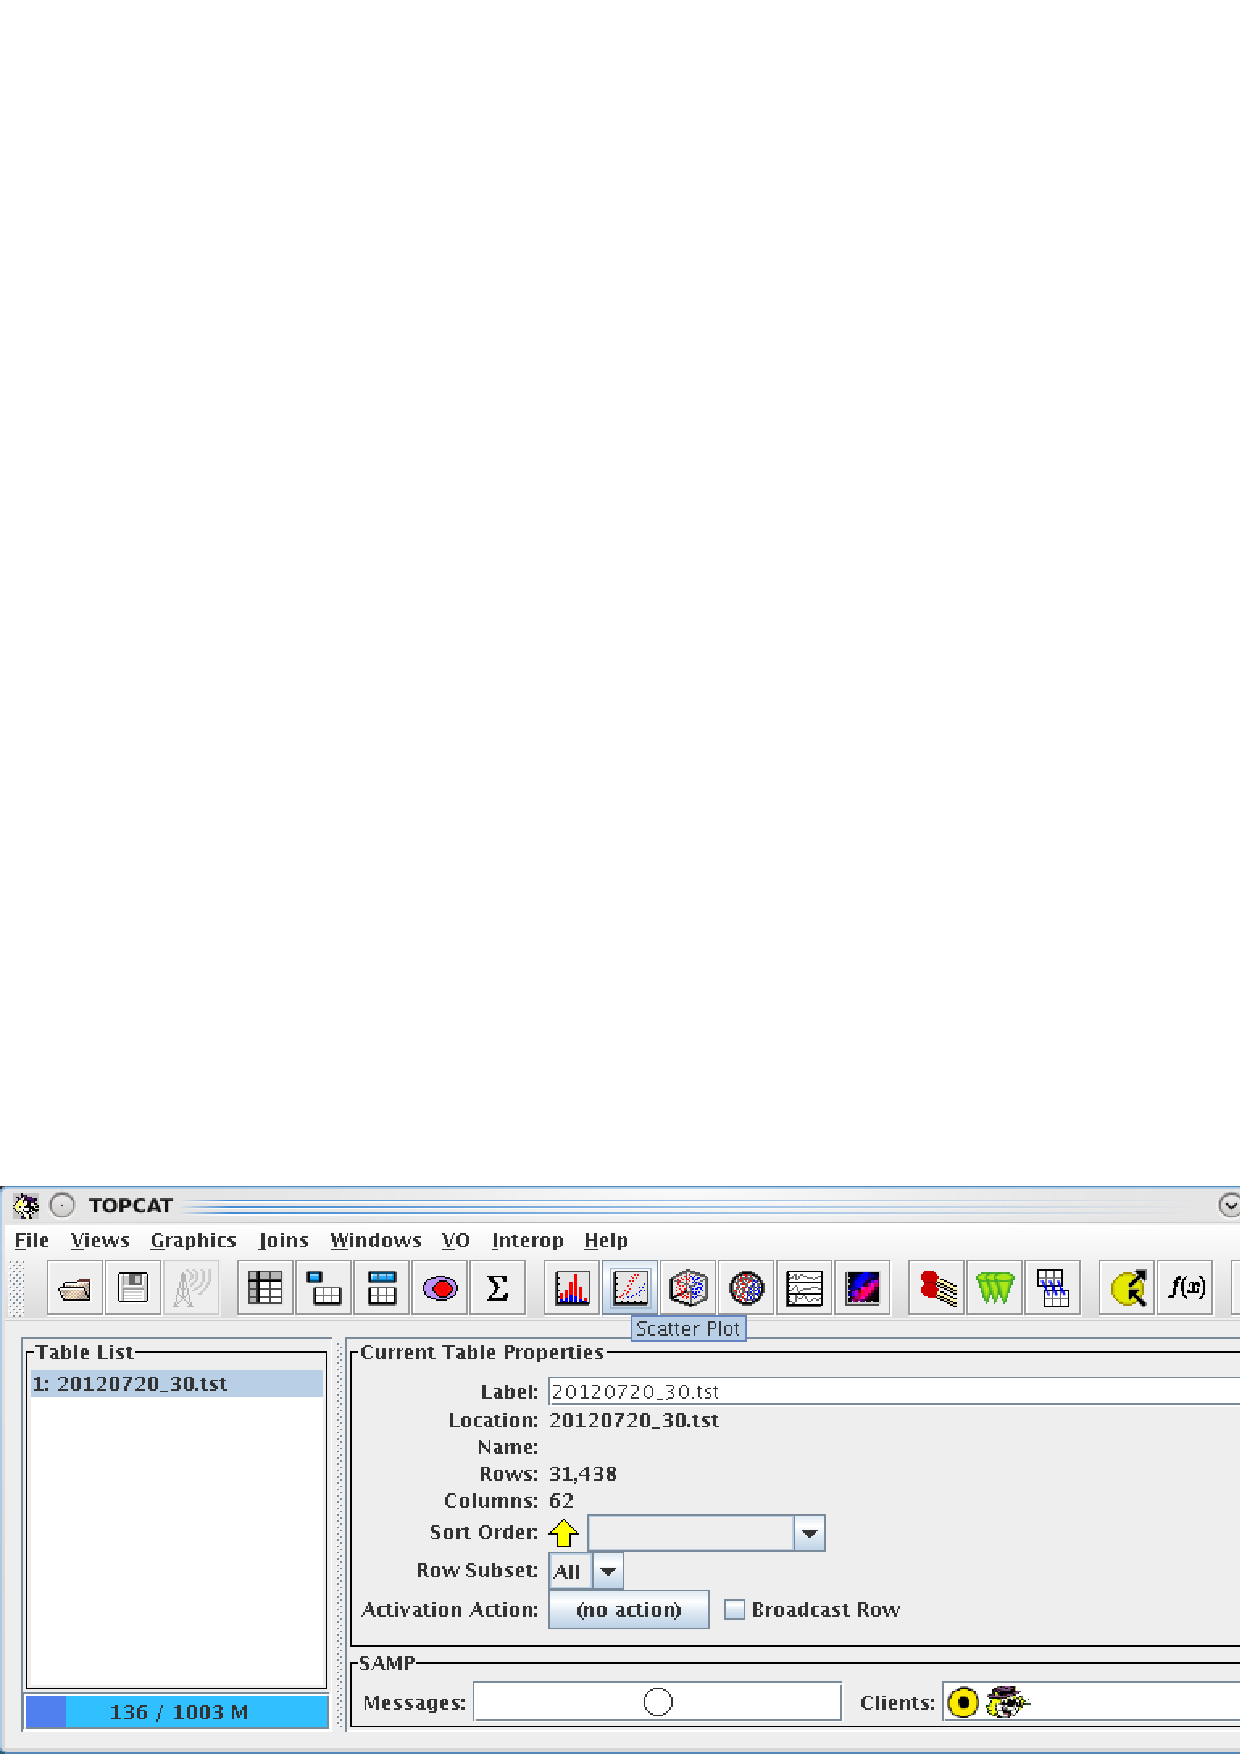
\includegraphics[width=0.95\textwidth]{sc21_topcat1}
\end{center}
\end{minipage}
\hspace{0.3cm}
\begin{minipage}[c]{0.32\linewidth}
In \topcat\ select the scatter plot option
from the menu bar across the top of the window.
\end{minipage}
\minipageclear
\vspace{0.5cm}

\begin{minipage}[c]{0.6\linewidth}
\begin{center}
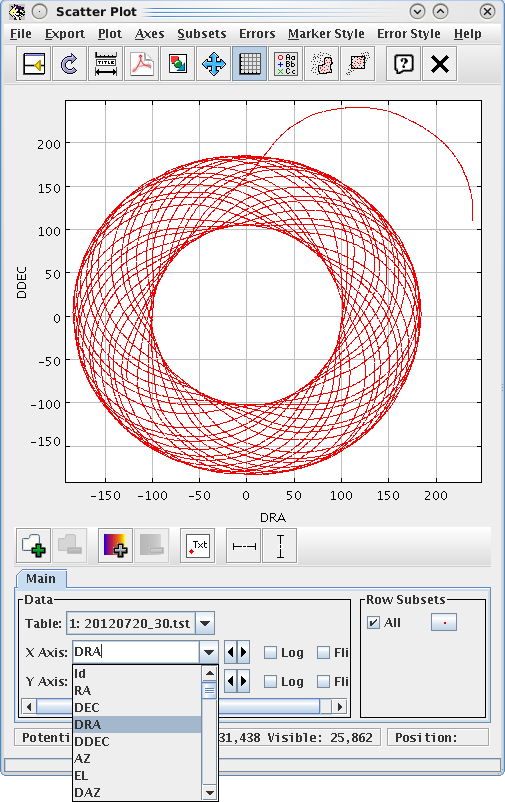
\includegraphics[width=0.75\textwidth]{sc21_topcat2}
\end{center}
\vspace{0.2cm}
\end{minipage}
\hspace{0.3cm}
\begin{minipage}[c]{0.32\linewidth}
With the scatter plot displayed you can adjust the $X$-axis and
$Y$-axis values to DRA and DDEC respectively to display the scan pattern.
If you are interested in seeing how any of the variables change over time,
select the the $X$ Axis to be either Id or RTS\_NUM.
\end{minipage}
\minipageclear

\end{fmpage}
\end{center}
\caption[Displaying the scan pattern with \topcat] { \small \topcat\
  example demonstrating how to display the scan pattern for an
  observation.  }
\label{fig:topcat}
\end{figure}


\section{\xlabel{scan_pat}Displaying scan patterns}
\label{sec:scan}

The movement of the telescope throughout a scan (as well as other
state information) is stored in the \texttt{MORE.SMURF.JCMTSTATE}
extension of a data file. The \smurf\ task \jcmtstate\ converts this
information into a simple ASCII tab-separated table.

\begin{terminalv}
% jcmtstate2cat s8a20120701_00008_*.sdf > state.tst
\end{terminalv}

Multiple files can be supplied to the command using standard shell
wild cards. If you have already concatenated your data you can simply
input the single concatenated file. It may be useful to view the scan
pattern for your observation, particularly for maps taken at high
elevations, to ensure the pattern completed successfully.


\begin{tip}
  Follow the \task{jcmtstate} command with \texttt{-h} to find out
  more information.
\end{tip}


This catalogue can be loaded into \topcat\ for plotting, making sure
to specify the TST format during loading.

\begin{terminalv}
% topcat -f tst state.tst
\end{terminalv}

Example of scan patterns displayed with \topcat\ can be seen in
\cref{Figure}{fig:scan}{telescope tracks}. Detailed instructions on
how to display the scan pattern for your observation are given in
\cref{Figure}{fig:topcat}{box below}.  All of the time-varying header
values are available for plotting. Other values include the azimuth
and elevation offsets (DAZ \& DEL), the WVM and 225\,GHz opacity
values, and the instrument temperatures (e.g.  SC2\_FPUTEMP gives the
temperature of the focal plane).

Due to extreme accelerations at ``turn-around'' points of a scan
pattern (especially for \textsc{pong}s), the telescope finds it hard
to follow the proscribed scan patterns at high elevations. To mitigate
this we try to avoid observing any sources above 70$^\circ$ elevation.
If the \fitslist\ keywords \param{ELSTART} and \param{ELEND}
indicate that your map was taken at high elevation you may consider
checking the success of the scan pattern. If you find your observation
has failed to follow the demanded scan pattern don't worry, the data are
likely to still be useful. This is especially true for \textsc{daisy}
maps where the high exposure-time central region is usually
unaffected.

\section{\xlabel{display_cube}Displaying time-series data}
\label{sec:gaiacube}

Use the \starlink\ application \textsc{Gaia} to visualise the
bolometer time-series data (or indeed \emph{any} SCUBA-2 data
file). This is initiated simply typing \texttt{gaia} into a terminal.

\begin{terminalv}
% gaia s8a20120725_00058_con.sdf
\end{terminalv}

Loading a file in \textsc{Gaia} produces two windows. The main window
(see \cref{Figure}{fig:gaia_main}{upper graphic}) shows a map of
bolometer values at a given point in time. The time slice displayed
may be changed by scrolling through the time axis. This is done in the
second window entitled \gaiathing{Display image sections of a
  cube}. The \gaiathing{Index of plane} slider towards the top of this
window may be moved to display different time slices in the main
window.

\starfig{sc21_gaia1}{[b]}{width=\linewidth}{fig:gaia_main}{
  Raw data displayed in the main \gaia\ window}{
  Initial \gaia\ windows displayed upon loading a data cube.
  The main window in the left shows a map of bolometer values at a fixed
  sample in time. You may have to zoom in multiple times by clicking the
  \gaiathing{Z} icon. On the right-hand side, the
  \gaiathing{Display image sections of a cube}
  dialogue enables you to navigate the time axis.
}

A third window will appear when you click on a bolometer---the
\gaiathing{Spectral plot} (see \cref{Figure}{fig:gaia_spec}{lower graphic}).
This shows an automatically scaled plot of the raw time stream of data for
that given bolometer. It will be overridden when you click on a different
bolometer.

\starfig{sc21_gaia2}{[t]}{width=0.8\linewidth}{fig:gaia_spec}{ \gaia\
  spectral plot window}{ The \gaiathing{Spectral plot} window displays
  the time-varying signal. This window appears automatically when a
  bolometer is clicked in the main window.  The vertical red line
  indicates the time slice that is currently selected in the
  \gaiathing{Display image sections of a cube} dialogue---this can be
  dragged across the spectrum to scroll through the time-slices.  }

A second way to scroll through the time axis is to click and drag the
vertical red bar on the \gaiathing{Spectral plot} window. As you do
so, the array shown in the main window will automatically update.

To highlight small variations between bolometers you will need to
change the auto cut and (depending on your preference) the colour
scheme---both are controlled by buttons on the sidebar.

See the \xref{\textsc{Gaia} manual}{sun214}{} for full
details.\footnote{\url{http://www.starlink.ac.uk/docs/sun214.htx/sun214.html}}


\section{\xlabel{regrid_map}Regridding data into a map}
\label{sec:regrid}

Any raw time-series data can be quickly regridded into sky frame
coordinates using the \smurf\ \makemap\ task in rebin mode. This
involves no further processing of the data. The following command produces
a map from the raw concatenated data; unlike the iterative mode of
\task{makemap} described in the next chapter, no configuration file is
required.

\begin{terminalv}
% makemap s8a20120725_00058_con.sdf crl2688_sky method=rebin spread=near
\end{terminalv}

The output map here is called \file{crl2688\_sky.sdf} and is shown in
\cref{Figure}{fig:regrid}{the figure below}.  The pixel scale is left
at the default values of 2\,arcsec on a side at 450$\mu$m and
4\,arcsec at 850$\mu$m (although this can be changed using the
\texttt{pixsize=}$x$ option on the command-line, where $x$ is in
arcsec).

\starfig{sc21_crl2688_regrid}{[b!]}{width=0.65\linewidth}{fig:regrid}{
  The regridded map of CRL~2688 displayed with \gaia.}{ The regridded
  map of CRL~2688 with the s8a sub-array displayed with \gaia.  }

\begin{tip}
  If you do not include \param{method=rebin}, the map-maker will
  default to \param{method=iterate}.
\end{tip}


\section{\xlabel{clean}Notes on cleaning your data}
\label{sec:clean}

Cleaning raw data is an essential first step towards making a quality
final map. The map-maker performs all of these cleaning steps during
the pre-processing stage. The commands for manually cleaning your data
are given in \cref{Appendix}{app:clean}{Cleaning the raw data}.  You
can also check out the SMURF SRO
Cookbook{\footnote{\url{http://www.starlink.ac.uk/docs/sc19.htx/sc19.html}}}
which goes into great depth on the data cleaning options.


\section{\xlabel{calcnoise}Checking the array performance}
\label{sec:calcnoise}

The on-sky performance of the array can be assessed using the \smurf\
command \calcnoise. Rather than give an absolute measure,
\task{calcnoise} should be used as an indicator of array performance
and stability.  \task{calcnoise} cleans the data then calculates the
white noise on the array (between 2 and 10\,Hz by default).
\begin{terminalv}
% calcnoise s8a20110720_00030\*.sdf s8a_noise power=!
\end{terminalv}
It will prompt for a configuration file to describe the cleaning
steps. The default is the file
\file{\$STARLINK\_DIR\allowbreak/share\allowbreak/smurf\allowbreak/dimmconfig\allowbreak\_calcnoise.lis} that is
included in \smurf. Two noise measurements are reported in the terminal:
the `Effective noise' and the `Effective NEP'.

An output file is created for each sub-array with the NEP map stored
in the \texttt{.MORE.SMURF.NEP} extension.

If you have a bright source in the field this will contaminate the
signal. In this case you should examine the \model{NOI} model from the
map-maker instead---see \cref{Section}{sec:models}{The individual
  models} for a description and \cref{Section}{sec:export}{Exporting
  individual models} for details on how to examine it.

\section{\xlabel{export}Exporting individual models}
\label{sec:export}

By default, the final values of the models fitted by the map-maker are
\emph{not} written out. However, this can be changed by setting
\xparam{EXPORTNDF}{exportndf} in the configuration file to the list of models
that you wish to view.
%\vspace{0cm}

\begin{terminalv}
exportndf = (com,gai,ast,flt,res,noi,qua)
\end{terminalv}

In addition to the models listed in \cref{Section}{sec:models}{The
individual models}, you can request \model{RES} in order to export the
\model{RES} model --- the residual signal remaining after
the other models have been removed.  If \model{NOI} (the estimate of
the bolometer noise levels) is exported, it is stored as the VARIANCE
component of the \model{RES} model; thus, export of \model{RES} is implied
if \model{NOI} is specified.

The \texttt{exportndf} parameter will write out the requested models
as NDF files with names based on the first input file that went into
the maps for each sub-array. This is first suffixed by \texttt{con},
indicating that several data files may have been concatenated
together. The three-letter code for each model is then appended to the
filename (such as \file{s8a20120720\_00030\_0003\_con\_com.sdf},
\file{s8a20120720\_00030\_0003\_con\_flt.sdf},
\file{s8a20120720\_00030\_0003\_con\_res.sdf})\footnote{The filename
shows the third sub-scan of Observation 30 since this is the first science
file that is encountered (see \cref{Chapter}{sec:raw}{Handling Raw
SCUBA-2 Data}).~} The variance and quality for the data are stored as
the VARIANCE and QUALITY components within the residual file NDF.

\begin{tip}
  These exported model components are 3-dimensional arrays with axes \texttt{
  (bolometer column, bolometer row, time slice index)}, and so can be viewed
  using the cube visualisation facilities within \gaia\ (see \gaiasun).
\end{tip}






\begin{thebibliography}{}
\addcontentsline{toc}{section}{References}

\bibitem{archibald}
Archibald,~E.~N., et~al, 2002, \htmladdnormallink{\textit{On the atmospheric limitations
of ground-based submillimetre astronomy using array receivers}}{http://dx.doi.org/10.1046/j.1365-8711.2002.05582.x}, MNRAS, 336, 1-13
(DOI:10.1046/j.1365-8711.2002.05582.x)

\bibitem{fellwalker}
Berry~D.~S.,  2015,
\htmladdnormallink{\textit{FellWalker - a Clump Identification Algorithm}}
{http://dx.doi.org/10.1016/j.ascom.2014.11.004},
Ast. \& Comp., 10, 22-31 (DOI:10.1016/j.ascom.2014.11.004)

\bibitem{oracdr}
Cavanagh~B., Jenness~T., Economou~F., Currie~M.~J., 2008,
\htmladdnormallink{\textit{The ORAC-DR data reduction
pipeline}}{http://dx.doi.org/10.1002/asna.200710944}, Astron. Nactr., 329, 295
(DOI:10.1002/asna.200710944)

\bibitem{smurf}
Chapin~E.~L., et~al., 2013, \textit{SMURF -- Sub-Millimetre User Reduction
Facility}, \xref{Starlink User Note 258}{sun258}{}

\bibitem{mapmaker}
Chapin~E.~L., et~al., 2013,
\htmladdnormallink{\textit{SCUBA-2: iterative map-making with the
Sub-Millimetre User Reduction Facility}}{http://dx.doi.org/10.1093/mnras/stt052},
MNRAS, 430, 2545 (DOI:10.1093/mnras/stt052)

\bibitem{ssds}
Currie~M.~J., Wallace~P.~T., Warren-Smith~R.~F., 1989,
\textit{Starlink Standard Data Structures}, \xref{Starlink General
Paper 38.2}{sgp38}{}

\bibitem{kappa}
Currie~M.~J., Berry~D.~S, 2013, \textit{KAPPA -- Kernel Application Package},
\xref{Starlink User Note 95}{sun95}{}

\bibitem{dempsey12}
Dempsey~J.~T. et al., 2013, \htmladdnormallink{\textit{SCUBA-2: on-sky calibration using
submillimetre standard sources}}{http://dx.doi.org/10.1093/mnras/stt090},
MNRAS, 430, 2534 (DOI:10.1093/mnras/stt090)

\bibitem{dempsey-spie}
Dempsey~J.~T., Friberg~P., Jenness~T., Bintley~D., Holland~W.~S., 2010
\htmladdnormallink{\textit{Extinction correction and on-sky calibration of
SCUBA-2}}{http://dx.doi.org/10.1117/12.856476},
Proc.\ SPIE, 7741 (DOI:10.1117/12.856476)

\bibitem{gaia}
Draper~P.~W., Gray~N., Berry~D.~S., Taylor~M., 2012,
\textit{GAIA -- Graphical Astronomy and Image Analysis Tool},
\xref{Starlink User Note 214}{sun214}{}

\bibitem{picard}
Gibb~A.~G., Jenness~T., Economou~F., 2012, \textit{PICARD --- a
PIpeline for Combining and Analyzing Reduced Data}
\xref{Starlink User Note 265}{sun265}{}

\bibitem{s2main}
Holland, W. S., et~al, 2013, \htmladdnormallink{\textit{SCUBA-2: The
10,000 pixel bolometer camera on the James Clerk Maxwell Telescope}}
{http://dx.doi.org/10.1093/mnras/sts612}, MNRAS, 430, 2513
(DOI:10.1093/mnras/sts612)

\bibitem{flux1}
Jenness~T., et~al, 2002, \htmladdnormallink{\textit{Towards the automated
reduction and calibration of SCUBA data from the James Clerk Maxwell
Telescope}}{http://dx.doi.org/10.1046/j.1365-8711.2002.05604.x},
MNRAS, 336, 14-21 (DOI:10.1046/j.1365-8711.2002.05604.x)

\bibitem{sc2ana005}
Scott~D., Van Engelen~A., 2005, \htmladdnormallink{\textit{Scan Mode Strategies for
SCUBA-2}}{http://docs.jach.hawaii.edu/JCMT/SC2/ANA/S210/005/sc2_ana_s210_005.ps},
SCUBA-2 Data Reduction document SC2/ANA/S210/005

\end{thebibliography}

\newpage
\appendix
\chapter{\xlabel{app_clean}Cleaning the raw data}
\label{app:clean}

You can use the \smurf\ task \clean\ to help inspect time-series.
\task{sc2clean} can be used to do two basic tasks in one go:
concatenate data (with or without applying a flatfield); and cleaning
(fix up steps and spikes, remove the means, filter, remove common-mode
etc.). It uses the same configuration files as the iterative map-maker
(though ignoring the map-making specific items).

In this first basic example, we just want to clean up some data enough
to see whether the bolometers have been flat-fielded correctly, and
more-or-less exhibit the same behaviour over time. The pre-processing
or cleaning steps used by default (\emph{i.e.} if ``\texttt{config=def}''
is included on the command line) are summarised in \cref{Table}{tab:dimmdef}{this
table}. Note, whilst it is not recommended to run \makemap\ in this way
(\emph{i.e.} without a configuration file), it is not so critical when running
\clean.

\begin{terminalv}
% sc2clean $FILES clean config=def
\end{terminalv}

Here \file{\$FILES} can just be a single file from a sub-array, or a
subset, e.g. \file{s8a20110417\_00051\_0003.sdf} (the first file
containing science data), \file{s8a20110417\_00051\_000"[1234]"} (File
1 is a noise observation with shutter closed that gets ignored, File 2
is a flatfield observation that will be used to override the flatfield
stored in the subsequent Files 3 and 4 which are concatenated
together, the \file{.sdf} is optional),
\file{s8a20110417\_00051\_000\textbackslash?} (Files 1 through 9),
\file{s8a20110417\_00051\_\textbackslash*} (the whole observation).

If you inspect the resulting \file{clean.sdf} in \gaia\
(\cref{Section}{sec:gaiacube}{Displaying time-series data}) and flip
through the data cube you should see all of the bolometers signals go
up and down together with about the same amplitude: the hope is that
for a well-behaved instrument you are mostly seeing sky noise
variations that are seen with roughly the same amplitude by all
bolometers.

Another common feature, if the scans are particularly long and/or fast
(e.g. 1\,degree across), is strong periodic signals that are
correlated with the scan pattern. See
\cref{Section}{sec:scan}{Displaying scan patterns}---in particular you
will want to plot \texttt{az} and \texttt{el} (the absolute azimuth
and elevation), and also \texttt{daz} and \texttt{del} (the azimuth
and elevation offsets from the map centre). This signal is usually
azimuth-correlated due to magnetic-field pickup. It only shows up in
azimuth, because the instrument is on a Nasmyth platform and therefore
does not move in elevation.

Part of the reason the signals look the same is because they have been
flatfielded. You can turn off flatfielding using the \param{noflat}
option to \task{sc2clean}, and you should then see that all of the
detector amplitudes vary.

Another very useful option is to remove the common signal observed by
all of the bolometers. This may be accomplished by

\begin{terminalv}
% sc2clean $FILES clean config='"compreprocess=1"'
\end{terminalv}

This \texttt{config} setting causes the default values to be used for all
configuration parameters except \xparam{COMPREPROCESS}{compreprocess},
which is set to 1 (the default is 0).  The residual signal left by this
command will exhibit second-order time-varying correlated signals across
the focal plane.  Usually these are not very large, but in some cases some
very large localized signals have been detected, particularly in the
850\,$\mu$m arrays in early 2011.

Another variation on this is to accentuate the residual low-frequency
noise by low-pass filtering the result. This can again be accomplished
by simply adding a filter command in the \param{config} parameter,
which in this case low-pass filters with a cutoff at 10\,Hz:

\begin{terminalv}
% sc2clean $FILES clean config='"compreprocess=1,filt_edgelow=10"'
\end{terminalv}

Finally, in some cases you might just want to fit and remove
polynomial baselines from the bolometers (by default only the mean is
removed). This example will remove a line, but you can increase the
value of \xparam{ORDER}{order} to remove higher-order polynomials

\begin{terminalv}
% sc2clean $FILES clean config='"order=1"'
\end{terminalv}

Non-default values for any of the cleaning parameter can be specified like so:
\begin{terminalv}
% sc2clean $FILES clean config='"order=1,dcfitbox=30,dcthresh=25,dcsmooth=50"'
\end{terminalv}
Or you can create your own customised configuration file. For instance:

\begin{terminalv}
% cat myconf
order=1
dcfitbox=30
dcthresh=25
dcsmooth=50
% sc2clean $FILES clean config=^myconf
\end{terminalv}

The more interesting pre-processing options that may be specified are listed
and described in \cref{Appendix}{app:parameters}{here}.





\newpage
\chapter{\xlabel{calib}SCUBA-2 data calibration}
\label{app:cal}

\section{\xlabel{fcf}Flux conversion factors (FCF)}
\label{app:fcf}

Primary and secondary calibrator observations have been reduced using
the specifically designed \file{dimmconfig\_bright\_compact.lis}.  The
maps produced from this are then analysed using tailor-made \picard\
recipes. For instructions on applying the FCFs to your map see
\cref{Section}{sec:cmult}{this page}.

A map reduced by the map-maker has units of pW. To calibrate the data
into units of janskys (Jy), a set of bright, point-source objects with
well-known flux densities are observed regularly to provide a flux
conversion factor (FCF). The data (in pW) can be multiplied by this
FCF to obtain a calibrated map. The FCF can also be used to assess the
relative performance of the instrument from night to night. The noise
equivalent flux density (NEFD) is a measure of the instrument
sensitivity, and while not discussed here, is also produced by the
\textsc{Picard} recipe shown here. For calibration of primary and
secondary calibrators, the FCFs and NEFDs have been calculated as
follows:

\begin{enumerate}
\item The \textsc{Picard} recipe \drrecipe{SCUBA2\_FCFNEFD} takes the
  reduced map, crops it, and runs background removal. Surface-fitting
  parameters are changeable in the \textsc{Picard} parameter file.

\item It then runs the \Kappa\ \beamfit\ task on the specified point
  source. The \task{beamfit} task will estimate the peak
  (uncalibrated) flux density and the FWHM. The integrated flux
  density within a given aperture (30-arcsec radius default) is
  calculated using \photom\ \autophotom. Flux densities for
  calibrators such as Uranus, Mars, CRL~618, CRL~2688 and HL~Tau are
  already known to \picard. To derive an FCF for other sources of
  known flux densities, the fluxes can be added to the parameter file
  with the source name (in upper case, spaces
  removed): \param{FLUX\_450.MYSRC~=~0.050}
  and \param{FLUX\_850.MYSRC~=~0.005} (where the values are in Jy),
  for example.

\item Three different FCF values are calculated, two of which are
  described below.

  \begin{enumerate}

  \item \textbf{The arcsecond FCF}
    \begin{equation}
      \label{eq:fcf_arcsec}
      \mathrm{FCF_{arcsec}} = \frac{S_{\mathrm{tot}}}{P_{\mathrm{int}} \times
        A_{\mathrm{pix}}}
    \end{equation}

    where $S_{\mathrm{tot}}$ is the total flux density of the
    calibrator, $P_{\mathrm{int}}$ is the integrated sum of the source
    in the map (in pW) and $A_{\mathrm{pix}}$ is the pixel area in
    arcsec$^2$, producing an FCF in Jy/arcsec$^2$/pW.

  \item\textbf{The beam FCF}
    \begin{equation}
      \label{eq:fcf_beam}
      \mathrm{FCF_{beam}} = \frac{S_{\mathrm{peak}}}{P_{\mathrm{peak}}}
    \end{equation}
    producing an FCF in units of Jy/beam/pW.
  \end{enumerate}

\end{enumerate}

The measured peak signal here is derived from the Gaussian fit of
\task{beamfit}. The peak value is susceptible to pointing and focus
errors, and we have found this number to be somewhat unreliable,
particularly at 450$\mu$m.


\section{\xlabel{extinction}Extinction correction}

Analysis of the SCUBA-2 secondary calibrators has allowed calculation
of the transmission relationships for the SCUBA-2 450\,$\mu$m and
850\,$\mu$m pass-bands to be determined. Full details of the analysis
and on-sky calibration methods of SCUBA-2 can be found in Dempsey et
al.\ (2013)~\cite{dempsey12}\cite{dempsey-spie}.

Archibald et al. (2002)\,\cite{archibald} describes how the Caltech
Submillimeter Observatory (CSO) 225\,GHz opacity, $\tau_{225}$,
relates to SCUBA opacity terms in each band, $\tau_{450}$ and
$\tau_{850}$. The JCMT water-vapour radiometer (WVM) uses the 183\,GHz
water line to calculate the precipitable water vapour (PWV) along the
line-of-sight of the telescope. This PWV is then input into an
atmospheric model to calculate the zenith opacity at 225\,GHz
($\tau_{225}$). This allows ease of comparison with the adjacent CSO
225\,GHz tipping radiometer. The opacities have been as:

\begin{equation}
\tau_{450} = 26.0 \times (\tau_{225} - 0.012);
\end{equation}
and
\begin{equation}
\tau_{850} = 4.6 \times (\tau_{225} - 0.0043).
\end{equation}

The SCUBA-2 filter characteristics are described in detail
\htmladdnormallinkfoot{on the JCMT
  website}{http://www.jach.hawaii.edu/JCMT/continuum/scuba2/filter/}.

The extinction correction parameters that scale from $\tau_{225}$ to
the relevant filter have been added to the map-maker code. You can
override these values by setting \param{ext.taurelation.filtname} in
your map-maker config files to the two coefficients `($a$,$b$)' that
you want to use (where \param{filtname} is the name of the
filter). The defaults are listed in
\file{\$SMURF\_DIR/smurf\_extinction.def}.

% It is worth noting that if an individual science map and
% corresponding calibrator observation has already been reduced with
% the old factors (and your source and calibrator are at about the
% same airmass and if the tau did not change appreciably), any errors
% in extinction correction should cancel out in the calibration.



\newpage
\chapter{\xlabel{calcrms}\drrecipe{SCUBA2\_CHECK\_RMS}}
\label{app:checkrmsparams}

The \picard\ recipe \drrecipe{SCUBA2\_CHECK\_RMS} estimates the RMS
and NEFD for a given observation via two methods to compare with
values from the SCUBA-2 integration time calculator (ITC).

The average NEP is calculated from the QL pipeline log file
(\file{log.nep}) corresponding to the date and wavelength. The FCF
(either from the file or the standard value) and mean transmission
over the observation is used to convert this to a zenith NEFD
(NEFD\_NEP). The elapsed time is used to convert that to an RMS noise
(RMS\_NEP).

The input images are cropped to the given size (as specified in the
FITS headers or via the MAP\_HEIGHT and MAP\_WIDTH recipe parameters)
before the mean exposure time is derived, along with the mean/median
noise and NEFD (RMS\_MAP and NEFD\_MAP).

The RMS corresponding to the observation type is calculated from the
SCUBA-2 ITC (RMS\_ITC); the time is used to convert that to a
corresponding NEFD (NEFD\_ITC).

The parameters written out to \file{log.checkrms} are listed below:
\begin{table}[h!]
  \begin{center}
    \begin{tabular}{|p{2.5cm}|p{12cm}|}
      \hline
      \textbf{Parameter} & \textbf{Description}\\
      \hline
      UT & UT date including day fraction\\
      Source & object name, upper case with spaces removed\\
      Obs & observation number\\
      FILTER & filter (wavelength)\\
      telapsed & elapsed time of observation in seconds\\
      texp & mean exposure time, derived from EXP\_TIME NDF component (sec)\\
      trans & mean line-of-sight transmission\\
      nep\_av & mean NEP for current observation (W/sqrt(Hz))\\
      nep\_av\_err & uncertainty in nep\_av (W/sqrt(Hz))\\
      rms\_nep & RMS derived from nefd\_nep (mJy/beam)\\
      nefd\_nep & NEFD derived from nep\_av and scaled elapsed time (mJy sqrt(sec))\\
      rms\_map & RMS noise in map, obtained from median of error array (mJy/beam)\\
      nefd\_map & NEFD derived from combination of variance and exposure time images (mJy sqrt(sec))\\
      rms\_itc & RMS noise estimated by SCUBA-2 integration time calculator (ITC) (mJy/beam) \\
      nefd\_itc & NEFD derived from rms\_itc and scaled elapsed time (mJy sqrt(sec)) \\
      itc\_obstype & observation type used by the ITC to derived RMS\\
      rms\_ratio & ratio of rms\_map to rms\_itc\\
      El & mean elevation in degrees\\
      CSO & mean zenith optical depth at 225 GHz, derived from WVM\\
      Tau & mean zenith optical depth at the current wavelength (given by FILTER above)\\
      Radius & radius in arcsec of image used in analysis\\
      pixscale & pixel scale in arcsec\\
      f & ITC f parameter\\
      project & project ID\\
      \hline
    \end{tabular}
  \end{center}
\end{table}




\newpage
\chapter{\xlabel{matchedfilter}SCUBA-2 Matched Filter}
\label{app:mf}

In order to optimally find sources that are the size of the telescope
beam, and suppress this residual large-scale noise, the \picard\
recipe \drrecipe{SCUBA2\_MATCHED\_FILTER} may be used. If there were
no large-scale noise in the map, the filtered signal map would be
calculated as follows:

\begin{equation}
  {\cal{M}} = \frac{[M(x,y)/\sigma^2(x,y)] \otimes P(x,y)}
  {[1/\sigma^2(x,y)] \otimes [P^2(x,y)]},
\end{equation}

where $M(x,y)$ and $\sigma(x,y)$ are the signal and RMS noise maps
respectively produced by \smurf, and $P(x,y)$ is a map of the
PSF. Here \(\otimes\)
denotes the 2-dimensional cross-correlation operator. Similarly, the
variance map would be calculated as

\begin{equation}
  {\cal{N}}^2 = \frac{1}{[1/\sigma^2(x,y)] \otimes [P^2(x,y)]}.
\end{equation}

This operation is equivalent to calculating the maximum-likelihood fit
of the PSF centered over every pixel in the map, taking into account
the noise. Presently $P(x,y)$ is simply modelled as an ideal Gaussian
with a FWHM set to the diffraction limit of the telescope.

However, since there is large-scale (and therefore correlated from
pixel to pixel) noise, the recipe also has an additional step. It
first smooths the map by cross-correlating with a larger Gaussian
kernel to estimate the background, and then subtracts it from the
image. The same operation is also applied to the PSF to estimate the
effective shape of a point-source in this background-subtracted map.

Before running \textsc{Picard}, a simple parameters file called
\file{smooth.ini} may be created.
\begin{terminalv}
[SCUBA2_MATCHED_FILTER]
SMOOTH_FWHM = 15
\end{terminalv}
%
where \param{SMOOTH\_FWHM~=~15} indicates that the background should
be estimated by first smoothing the map and PSF with a 15~arcsec FWHM
Gaussian. The recipe is then executed as follows:
%
\begin{terminalv}
% picard -recpars smooth.ini SCUBA2_MATCHED_FILTER map.sdf
\end{terminalv}
%
The output of this operation is a smoothed image called
\file{map\_mf.sdf}. By default, the recipe automatically normalizes
the output such that the peak flux densities of point sources are
conserved. Note that the accuracy of this normalization depends on how
closely the real PSF matches the 7.5~arcsec and 14~arcsec full-width
at half-maximum (FWHM) Gaussian shapes assumed at 450$\mu$m and
850$\mu$m, respectively (an explicit PSF can also be supplied using
the \param{PSF\_MATCHFILTER} recipe parameter).




\newpage
\chapter{\xlabel{fcfsred}FCFs by reduction date}
\label{app:fcfs}

Ongoing development of the SCUBA-2 analysis has resulted in ongoing
changes to the atmospheric opacity relationships and the FCFs. 
Depending on when your data were reduced you will need to apply 
different calibration values. \textsc{orac-dr} will automatically apply
the appropriate values. 

\textbf{Note:} As of the 2021A Starlink release, the
opacity relations and FCF values have been updated following the
results presented by Mairs et al. 2021 \cite{mairs21}. Historical values derived by Dempsey et al. 2013
\cite{dempsey12} are presented below the updated values for comparison.

\vspace{1cm}

\textbf{Explanation of parameters} (see also Appendix \ref{app:cal}):

Starlink currently applies the following multiplicative extinction correction to SCUBA-2 data:

\begin{equation}
\mathrm{Extinction\:Correction} = \frac{1}{\mathrm{exp}[-\tau_{\nu}\times\mathrm{Airmass}]}
\end{equation}
where $\tau_{\nu}$ is the atmospheric opacity at the given frequency, $\nu$. ``Opacity relations''  
relate the measured $\tau_{225}$ to the atmospheric opacity at the operating frequencies of 
SCUBA-2, $\tau_{666}$ (450~$\mu$m) and $\tau_{345}$ (850~$\mu$m). Their form is:
\begin{equation}
\label{eq:2021taurelation}
\tau_{\nu} = \mathrm{a}\times(\tau_{225,\mathrm{zen}} + \mathrm{b} + \mathrm{c}\times\sqrt{\tau_{225,\mathrm{zen}}}),
\end{equation}
where a, b, and c are empirically derived coefficients (see Mairs et al 2021 \cite{mairs21}).
You can find out what opacity relation was applied by using the \Kappa\ command \hislist.

\begin{terminalv}
%  hislist file | grep EXT.TAURELATION
\end{terminalv}

This will return something like the following,
\begin{terminalv}
      EXT.TAURELATION.450=(23.3,-0.018,0.05),
      EXT.TAURELATION.850=(3.71,-0.040,0.202), EXT.TAUSRC=auto, FAKESCALE=1,
\end{terminalv}
indicating, for example, that at 850~$\mu$m, a=3.71, b=-0.040, and c=0.202.

\vspace{5mm}

There are two commonly used FCF types:
\begin{itemize}
\item Peak FCF (Jy/pW/beam)---multiply your map by this when you wish
to measure absolute peak fluxes of discrete sources.
\item Arcsec FCF (Jy/pW/arcsec$^2$)---multiply your map by this if
you wish to use the calibrated map to do aperture photometry/extended source flux recovery.
\end{itemize}

\textbf{Note:} The FCFs are applied after the extinction correction, so the values are intrinsically
related to one another. The proper extinction correction must be applied before using the FCF
values presented below.

\newpage

\textbf{Results from Mairs et al 2021 \cite{mairs21}. Employed by default in Starlink versions 2021A and after. Dates are inclusive. See Figure~\ref{fig:FCFstep}}\\
\begin{table}[h!]
\begin{center}
\begin{tabular}{|l|c|c|c|c|}
 \hline
 \multicolumn{1}{|c|}{Date} &
 \multicolumn{2}{c|}{FCF - 450$\mu$m} &
 \multicolumn{2}{c|}{FCF - 850$\mu$m} \\
\cline{2-5}
& Jy/pW/beam &Jy/pW/arcsec$^2$ & Jy/pW/beam &Jy/pW/arcsec$^2$ \\
 \hline
until 30 April 2011 &383  & 4.9 &1080 &5.0 \\
1 May 2011 - 1 Nov 2016 & $531\pm93$ & $4.61\pm0.60$ & $525\pm37$ & $2.25\pm0.13$ \\
2 Nov 2016 - 29 June 2018 & $531\pm93$ & $4.61\pm0.60$ & $516\pm42$ & $2.13\pm0.12$ \\
30 June 2018 Onwards & $472\pm76$ & $3.87\pm0.53$ & $495\pm32$ & $2.07\pm0.12$ 
 \\
\hline
\end{tabular}
\end{center}
\end{table}

From 1 May 2011 onwards, the a, b, and c values presented in the table below correspond to Equation \ref{eq:2021taurelation}:\\
\begin{table}[h!]
\begin{center}
\begin{tabular}{|l|c|c|}
 \hline
 \multicolumn{1}{|c}{Date} & \multicolumn{2}{|c|}{Opacity Relation}  \\ \cline{2-3}
                           & 450$\mu$m  & 850$\mu$m \\ \hline
until 30 April 2011 & 32 $\times$ ($\tau_{225}$ - 0.02)    & 5.2 $\times$ ($\tau_{225}$ - 0.013)  \\
1 May 2011 Onwards & \begin{tabular}[c]{@{}c@{}c@{}c@{}}\\a=23.3$\pm$1.5\\b=-0.018$\pm$0.006\\c=0.05$\pm$0.04\end{tabular}& \begin{tabular}[c]{@{}c@{}c@{}c@{}}\\a=3.71$\pm$0.18\\b=-0.040$\pm$0.008\\c=0.202$\pm$0.044\end{tabular}\\
\hline
\end{tabular}
\end{center}
\end{table}

\begin{center}
\begin{figure}
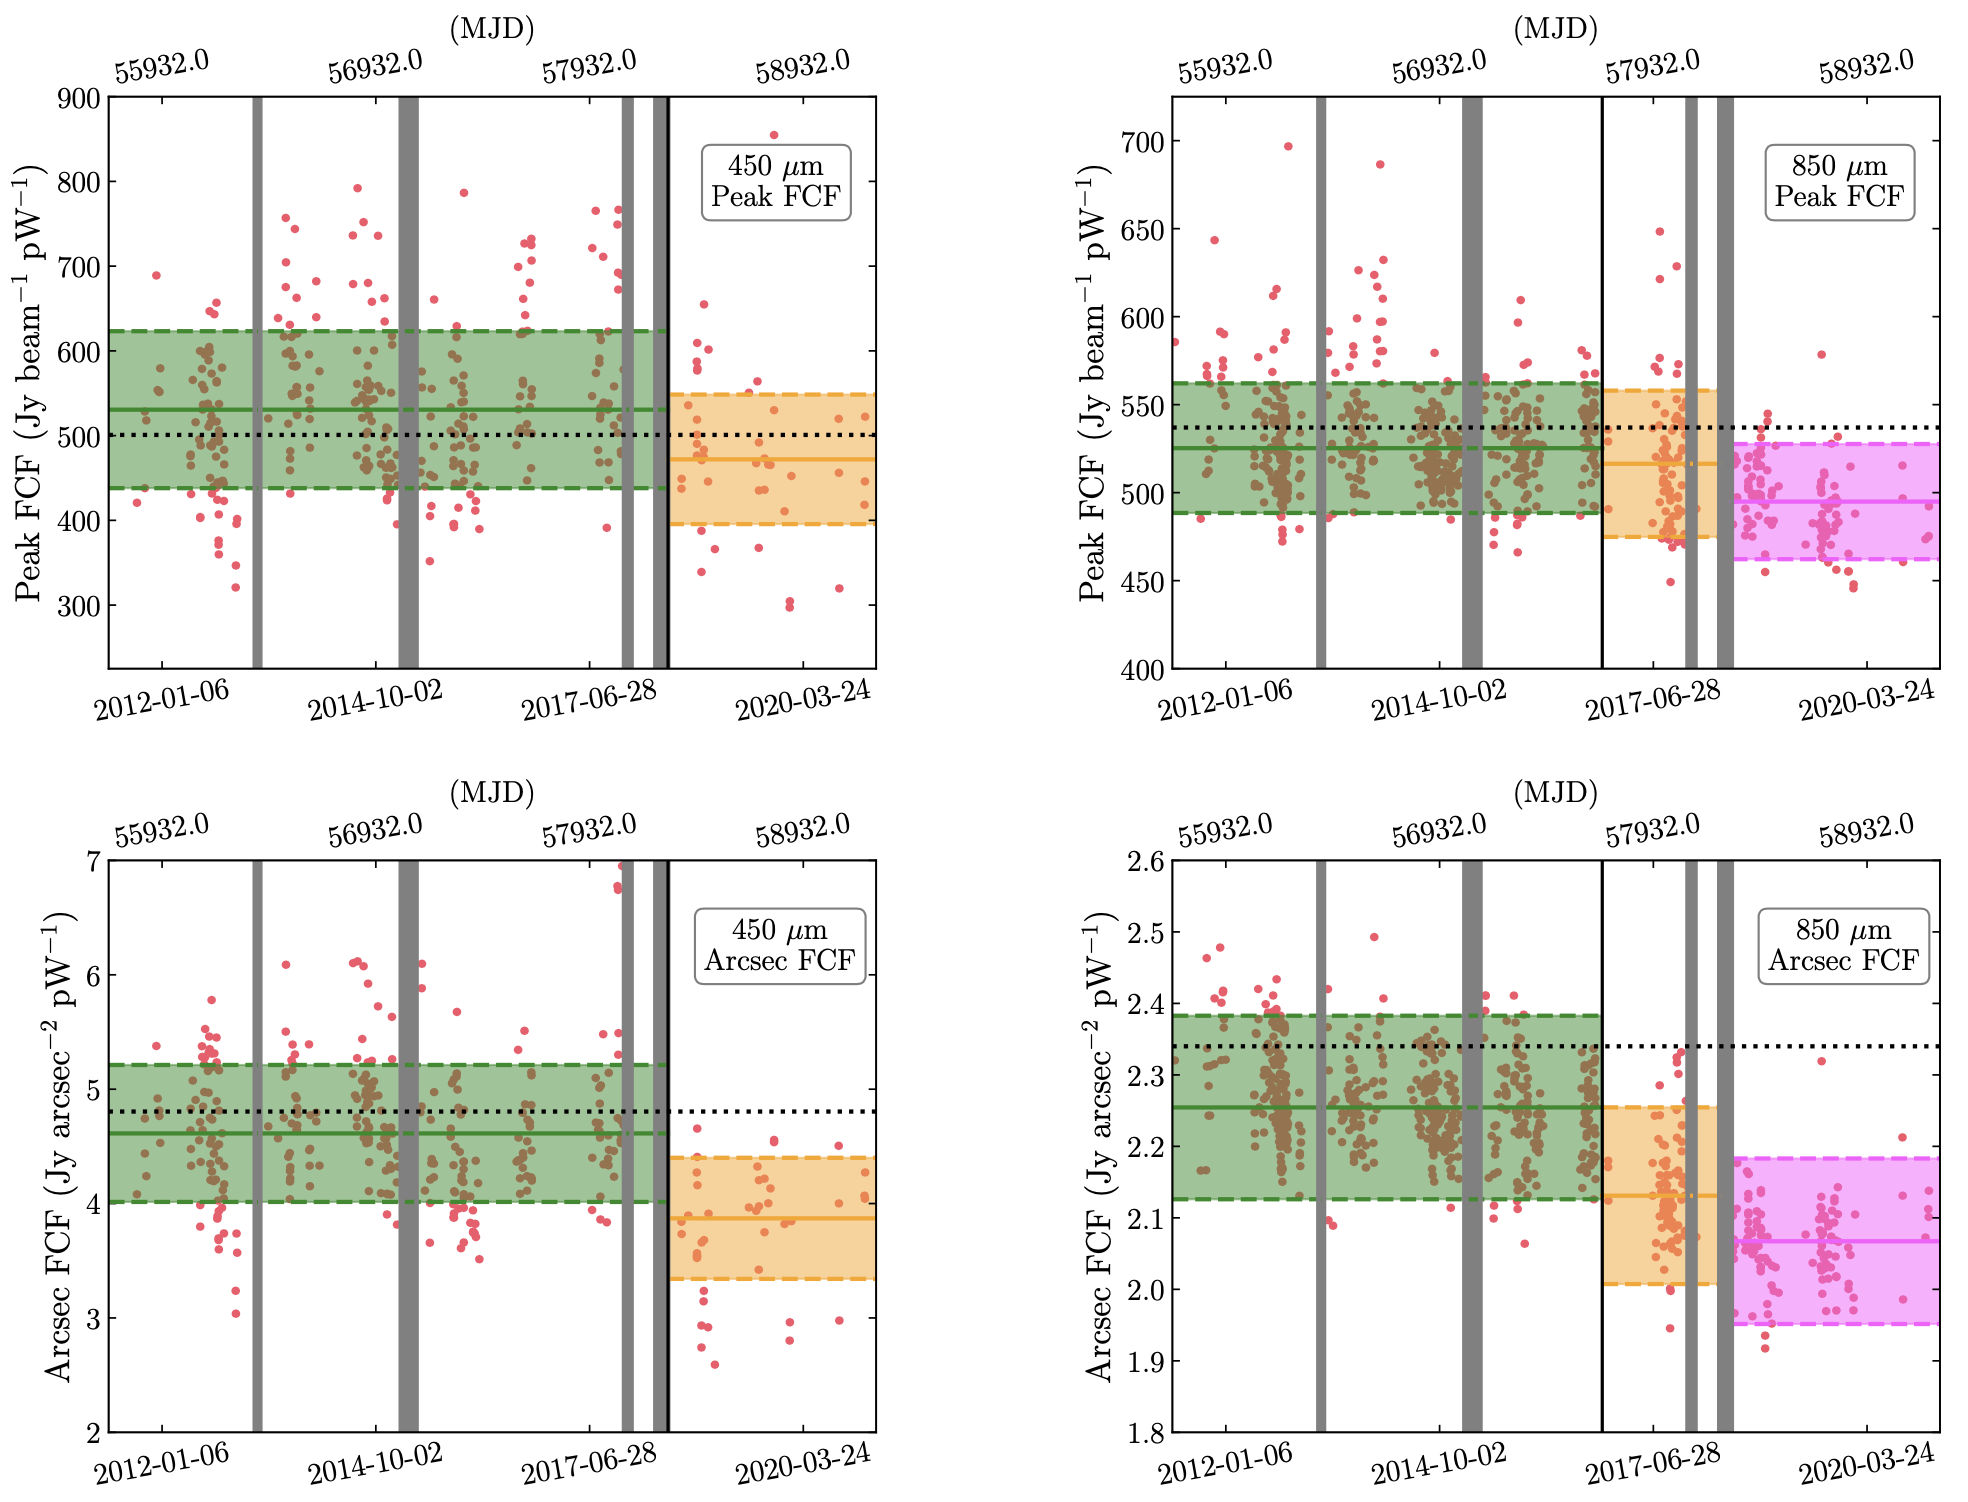
\includegraphics[width=0.9\linewidth]{sc21_FCFstep}
\caption[FCF step function]{From Mairs et al (2021)~\cite{mairs21}. FCFs derived using flux measurements of the primary calibrator Uranus during the stable part of the night (07:00-17:00 UTC) as a function of date. The gray shaded regions indicate epochs that are not included in the FCF determinations. The horizontal, shaded regions indicate the median FCF value over each span of time and the associated median absolute deviation added in quadrature with the 5\% uncertainty in the Uranus flux model. The black (dotted) lines indicate the original FCF value derived by Dempsey et al (2013)~\cite{dempsey12}, adjusted for the newly derived opacity relations, assuming the most common atmospheric transmissions during observations (see Figure 2). Left: Peak (Top) and Arcsecond (Bottom) FCFs derived at 450 microns. The solid, vertical line at the right edge of the latest gray region marks 2018 June 30 when the secondary mirror unit maintenance was completed. Data wherein the atmospheric transmission are less than 10\% are excluded. Right: Peak (Top) and Arcsecond (Bottom) FCFs derived at 850 microns. The solid, vertical line marks 2016 November, when the SCUBA-2 thermal filter stack was updated. Data wherein the atmospheric transmission are less than 25\% are excluded..}
\label{fig:FCFstep}
\end{figure}
\end{center}

\rule{1.0\textwidth}{2pt}

\textbf{Results from Dempsey et al. 2013 \cite{dempsey12}: employed by default in Starlink versions 2018A and previous.}\\
\begin{table}[h!]
\begin{center}
\begin{tabular}{|l|c|c|c|c|}
 \hline
 \multicolumn{1}{|c|}{Date} &
 \multicolumn{2}{c|}{FCF - 450$\mu$m} &
 \multicolumn{2}{c|}{FCF - 850$\mu$m} \\
\cline{2-5}
& Jy/pW/beam &Jy/pW/arcsec$^2$ & Jy/pW/beam &Jy/pW/arcsec$^2$ \\
 \hline
until January 2012 &383  & 4.9&1080 &5.0 \\
January 2012 - July 2012&606&6.06 &556 &2.42 \\
July 2012 onwards&491 &4.71 &537 &2.34 \\
\hline
\end{tabular}
\end{center}
\end{table}
\vspace{-2mm}
\begin{table}[h!]
\begin{center}
\begin{tabular}{|l|c|c|}
 \hline
 \multicolumn{1}{|c}{Date} & \multicolumn{2}{|c|}{Opacity Relation}  \\ \cline{2-3}
                           & 450$\mu$m  & 850$\mu$m \\ \hline
until January 2012       & 32 $\times$ ($\tau_{225}$ - 0.02)    & 5.2 $\times$ ($\tau_{225}$ - 0.013)  \\
January 2012 - July 2012 & 26 $\times$ ($\tau_{225}$- 0.01923)  & 4.6 $\times$ ($\tau_{225}$ - 0.00435)  \\
July 2012 onwards        & 26 $\times$ ($\tau_{225}$ - 0.01196) & 4.6 $\times$ ($\tau_{225}$ - 0.00435)  \\
\hline
\end{tabular}
\end{center}
\end{table}

\newpage
\chapter{\xlabel{cog}Aperture-photometry Curve of Growth}
\label{app:cog}

The SCUBA-2 beam has a broad error beam. As the size of the annulus
changes, the contribution from the error beam scales according to the
curve-of-growth---see \cref{Figure}{fig:cog}{the figure below}. To correct for an
aperture size differing from 60-arcsec diameter you should read off the
appropriate scaling factor for your FCF from the graph below.

\starfig{sc21_curveofgrowth}{[h!]}{width=\linewidth}{fig:cog}{
  Aperture photometry curve of growth}{
  Aperture photometry curve of growth normalised for a 60-arcsec
  aperture at 450$\mu$m \textbf{(left)} and 850$\mu$m
  \textbf{(right)}. Figure taken from Dempsey et al. (2013).
}


\newpage
\chapter{\xlabel{fits}Convert format from FITS to NDF}
\label{app:fits}

It is often useful to utilise data from other wavelengths or
instruments (either for a comparison or for an external mask). In the
following example, the FITS file called \file{file.fits} is
converted to NDF format as \file{file.sdf} using the \starlink\
package \convert. Note that the \file{.sdf} file extension NDF may
be omitted to save typing.

\begin{terminalv}
% convert
% fits2ndf file.fits file.sdf
\end{terminalv}

FITS files from certain recognised sources have special rules applied
when converting from FITS to NDF, as described in the documentation for
\xref{\task{fits2ndf}}{sun55}{FITS2NDF}. For FITS files from other sources, the
primary array in the FITS file is stored as the main NDF in the output
file. Any FITS extensions present in the FITS file will be placed into
NDF extensions called FITS\_EXT\_$<n>$, where $n$ counts from one for
the first FITS extension.  To see a list of the extension NDFs in
\file{fred.sdf}, do:

\begin{terminalv}
% ndfecho fred.more
fred.MORE.FITS_EXT_1
fred.MORE.FITS_EXT_2
fred.MORE.FITS_EXT_3
\end{terminalv}

When running a \textsc{Kappa} ot \textsc{smurf} command, you can refer
to these extension just as they are listed above. So for instance:

\begin{terminalv}
% ndftrace fred.MORE.FITS_EXT_1

   NDF structure /home/dsb/fred.MORE.FITS_EXT_1:
      Units:  COUNTS/S

   Shape:
      No. of dimensions:  2
      Dimension size(s):  270 x 263
      Pixel bounds     :  1:270, 1:263
      Total pixels     :  71010
...
...
\end{terminalv}

Alternatively, you can copy the NDF into its own separate file:

\begin{terminalv}
% ndfcopy in=fred.MORE.FITS_EXT_1 out=new_file
\end{terminalv}

If one of the extensions contains a variance array that you would like to
as the \texttt{Variance} component of the main NDF, a command like the
following will do that:

\begin{terminalv}
% setvar ndf=new_file from=fred.MORE.FITS_EXT_2
\end{terminalv}

The \task{fits2ndf} command offers a way of mapping FITS extensions to
familiar NDF array components DATA, VARIANCE, and QUALITY
through the \param{EXTABLE} file, avoiding the \ndfcopy\ and possible
\setvar\ steps.

You can convert an NDF to a FITS file using the command
\xref{\task{ndf2fits}}{sun55}{NDF2FITS}:

\begin{terminalv}
% convert
% ndf2fits file.sdf file.fits
\end{terminalv}





\newpage
\chapter{\xlabel{selpars}Configuration-parameter Descriptions}
\label{app:parameters}

This appendix describes some of the \makemap\ configuration parameters
that are more likely to be of interest to a typical user. Thus parameters
relating to experimental or deprecated features, or features that should
not normally need to be changed, are not included here. For a complete list
of all available configturation parameters, see
\xref{SUN/258}{sun258}{par_full}.

\begin{itemize}
\item The ``SMURF Usage'' section of each description lists the \SMURF commands
that accept the parameter. This does not mean that all the
listed commands actually \emph{use} the parameter---it just means that
any commands \emph{not} in the list will report an error if the parameter
is supplied.
\item The default value for each parameter is shown in square brackets at
the end of the description. These default values are defined in the file
\texttt{\$SMURF\_DIR/smurf\_makemap.def} and are the values that are used
for any parameters that are not assigned a value within the configuration
file supplied to \makemap. In other words, any parameter values supplied
within a configuration file will be used instead of these default values.
\end{itemize}
\ifpdf
\else
~\newline
\textbf{\large Alphabetical listing:} \newline
See \cref{Appendix}{app:catpars}{Configuration parameters listed by
category} for classified listings.
\fi

\sstminitoc{}
\sstnomaintoc
% This file was created using:
%
%	applications/smurf/defaults/make_pardocs \
%		selected_params.lis \
%		selected_params.tex \
%		../../../applications/smurf/defaults 
%


\section{General Iterative }
\sstminitoc{}


\sstroutine{
   NUMITER
}{
   Determines when to stop iterating
}{
   \sstdescription{
      If a positive number is supplied, the specified number of
      iterations will always be performed. If a negative number is
      supplied, the absolute value gives the maximum number of
      iterations to perform. Fewer iterations will be performed if
      the termination criteria specified by parameter {\tt{"}}\xref{maptol}{sun258}{MAPTOL}{\tt{"}} and
      parameter {\tt{"}}\xref{chitol}{sun258}{CHITOL}{\tt{"}} are both met before {\tt{"}}-numiter{\tt{"}}
      iterations have been performed. [-5]
   }
   \sstattributetype{
      real
   }
   \sstdiytopic{
      SMURF Usage
   }{
      MAKEMAP, CALCQU
   }
}

\sstroutine{
   MAPTOL
}{
   Specifies when to stop iterating
}{
   \sstdescription{
      If the normalised change (either the mean or maximum change -
      see parameter {\tt{"}}\xref{maptol\_mean}{sun258}{MAPTOL_MEAN}{\tt{"}}) between the maps created on
      subsequent iterations falls below the value of maptol, then the
      map-maker performs one more iteration and then terminates. Only
      used if parameter {\tt{"}}\xref{numiter}{sun258}{NUMITER}{\tt{"}} is negative. The normalised mean
      (or maximum) change between maps is defined as the mean (or
      maximum) of the absolute change in map pixel value, taken
      over all pixels within the region of the AST mask (if any,
      see parameter {\tt{"}}\xref{ast.zero\_mask}{sun258}{AST.ZERO_MASK}{\tt{"}}, etc), and normalised by the RMS
      of the square root of the pixel variances. Compared to parameter
      {\tt{"}}\xref{chitol}{sun258}{CHITOL}{\tt{"}}, this is much more like a {\tt{"}}by eye{\tt{"}} test, that will stop
      the solution when the map stops changing. [0.05]
   }
   \sstattributetype{
      real
   }
   \sstdiytopic{
      SMURF Usage
   }{
      MAKEMAP, CALCQU
   }
}


\sstroutine{
   MODELORDER
}{
   Determines which models to include in the iterative
   process, and the order in which they are evaluated
}{
   \sstdescription{
      This should be a comma-separated list, in parentheses,
      containing one or more of the following model names, in the
      order in which they should be evaluated. Note: components
      specified AFTER 'ast' will not be calculated for the first
      time until the second iteration:

      \sstitemlist{

         \sstitem
         dks: fit and remove dark squid for the column

         \sstitem
         com: remove common-mode signal

         \sstitem
         gai: if com specified, fit gain/offset of common mode

         \sstitem
         ext: apply extinction correction

         \sstitem
         ast: estimate the map and astronomical signal

         \sstitem
         flt: apply filter to time streams

         \sstitem
         noi: estimate time-domain variance

         \sstitem
         smo: time series smoothing using a median or mean boxcar filter

         \sstitem
         ssn: scan-synchronous (i.e. azimuth dependent) noise removal

         \sstitem
         pln: remove plane from each time slice

         \sstitem
         tmp: remove externally define template such as azimuth [(com,gai,ext,flt,ast,noi)]
      }
   }
   \sstattributetype{
      list of strings
   }
   \sstdiytopic{
      SMURF Usage
   }{
      MAKEMAP, CALCQU
   }
}

\sstroutine{
   EXPORTNDF
}{
   Provides diagnostic information
}{
   \sstdescription{
      Specify a value of 1 or 0 to export all or none of the
      model components after the final iteration. You can also
      specify a comma-separated list of component names, enclosed
      in parentheses, to be exported. Note that you can specify
      additional components RES and QUA to what may be provided to
      parameter {\tt{"}}\xref{modelorder}{sun258}{MODELORDER}{\tt{"}} if you wish to export the residual
      model or quality arrays respectively. Exportation of RES is
      implied if NOI is specified as it becomes the variance
      component of the resulting NDF for RES. QUA will become the
      quality component of any full 3-dimensional model (e.g.
      RES, AST, FLT, EXT), but no quality will be written to model
      components with different dimensions. [0]
   }
   \sstattributetype{
      integer or list of strings
   }
   \sstdiytopic{
      SMURF Usage
   }{
      MAKEMAP, CALCQU
   }
}


\sstroutine{
   ITERMAP
}{
   Provide extra diagnostic information
}{
   \sstdescription{
      If itermap is set to a positive value, the map from each iteration
      of each chunk will be stored in an output NDF. If itermap is set
      to a negative value, only the final iteration will be written from
      each chunk. If its absolute value is larger than 1, then each
      itermap will include a quality component that reflects the AST
      mask in use.

      By default, each itermap NDF will be stored in an extension
      called .MORE.SMURF.ITERMAPS in the main output NDF. However,
      an alternative location can be specified by supplying a value
      for ADAM parameter ITERMAPS. This is useful as it allows you
      to look at earlier itermaps whilst makemap is still running. [0]
   }
   \sstattributetype{
      integer
   }
   \sstdiytopic{
      SMURF Usage
   }{
      MAKEMAP, CALCQU
   }
}

\sstroutine{
   BOLOMAP
}{
   Creates diagnostic information
}{
   \sstdescription{
      If non-zero, a separate map will be created from each
      individual bolometer. These maps are placed in the BOLOMAPS
      component of the SMURF extension in the main output map. [0]
   }
   \sstattributetype{
      integer
   }
   \sstdiytopic{
      SMURF Usage
   }{
      MAKEMAP, CALCQU
   }
}

\sstroutine{
   SHORTMAP
}{
   Provides extra diagnostic information
}{
   \sstdescription{
      If non-zero, then an extension called .MORE.SMURF.SHORTMAPS
      is added to the output map NDF, holding maps made from every
      group of {\tt{"}}shortmap{\tt{"}} adjacent time slices. Alternatively, set
      to -1 to produce a map each time the TCS\_INDEX value within
      the JCMTSTATE extension is incremented (i.e., each time a full
      pass through the scan pattern has been completed). Any other
      negative value is interpreted as a duration in seconds, and is
      converted to time slices using the (possibly down-sampled)
      sample frequency of the data being mapped. [0]
   }
   \sstattributetype{
      integer
   }
   \sstdiytopic{
      SMURF Usage
   }{
      MAKEMAP, CALCQU
   }
}


\sstroutine{
   HITSLIMIT
}{
   Rejects map pixels that receive very few samples
}{
   \sstdescription{
      If non-zero, pixels that receive very few bolometer samples
      are set to bad in the final map. The limiting number of
      bolometer samples is equal to {\tt{"}}hitslimt{\tt{"}} times the mean
      number of hits per pixel, averaged over the map pixels
      that recieve at least one bolometer sample. [0.01]
   }
   \sstattributetype{
      real
   }
   \sstdiytopic{
      SMURF Usage
   }{
      MAKEMAP, CALCQU
   }
}




\section{Preprocessing     }
\sstminitoc{}


\sstroutine{
   DOWNSAMPSCALE
}{
   Speeds up map-making, and reduces memory requirements
}{
   \sstdescription{
      If the telescope is scanning slowly the data may be
      safely down-sampled to save memory and time. This parameter
      controls the minimum angular scale on the sky. The new
      sample frequency is chosen such that this scale will be
      preserved taking into account the average slew speed and
      the sample rate of the input files. If a positive value is
      selected, this gives the angular scale (in arcsec) to which
      the new sample rate will be matched. Alternatively, if a
      negative value is supplied, its magnitude will be multiplied
      by the PIXSIZE for the requested map. For example, the default
      here is to set it to -1 such that the time-series sample rate
      matches the pixel grid (in practice, a factor of 2 might make
      more sense as this would correspond to the Nyquist frequency
      of the map pixel grid). [-1]
   }
   \sstattributetype{
      real
   }
   \sstdiytopic{
      SMURF Usage
   }{
      MAKEMAP, CALCQU
   }
}


\sstroutine{
   MAXLEN
}{
   Determines how the input time-series data is split into chunks
}{
   \sstdescription{
      The maximum length (in seconds) for a single chunk of
      concatenated data. If 0 is supplied, attempt to concatenate
      entire continuous chunks. [0]
   }
   \sstattributetype{
      integer
   }
   \sstdiytopic{
      SMURF Usage
   }{
      MAKEMAP, CALCQU
   }
}

\sstroutine{
   DOCLEAN
}{
   Allows pre-cleaned data to be used
}{
   \sstdescription{
      Set this to 0 to turn off all data cleaning operations
      prior to the start of iterative map-making. [1]
   }
   \sstattributetype{
      integer
   }
   \sstdiytopic{
      SMURF Usage
   }{
      MAKEMAP, CALCQU
   }
}


\sstroutine{
   EXPORTCLEAN
}{
   Allows the initial cleaned data to examined or saved for
   later use
}{
   \sstdescription{
      If non-zero, the data will be saved to an NDF immediately
      after data cleaning and before map-making. The NDF name will
      be the same as model components, except with the suffix
      {\tt{"}}\_cln{\tt{"}}. Even if parameter {\tt{"}}\xref{doclean}{sun258}{DOCLEAN}{\tt{"}} ise set to zero, the
      data will be exported immediately before map-making. [0]
   }
   \sstattributetype{
      integer
   }
   \sstdiytopic{
      SMURF Usage
   }{
      MAKEMAP, CALCQU
   }
}


\sstroutine{
   ORDER
}{
   Baseline removal
}{
   \sstdescription{
      Subtract a baseline polynomial of this order as part of
      the initial cleaning phase. [1]
   }
   \sstattributetype{
      integer
   }
   \sstdiytopic{
      SMURF Usage
   }{
      SC2CLEAN, CALCQU, MAKEMAP
   }
}


\sstroutine{
   COMPREPROCESS
}{
   Remove common-mode before the iterative algorithm begins
}{
   \sstdescription{
      If non-zero, the common-mode will be estimated and removed
      additionally as a pre-processing step. All the {\tt{"}}com.$<$xxx$>${\tt{"}} and
      {\tt{"}}gai.$<$xxx$>${\tt{"}} parameters are parsed and used (e.g., to also
      flag bad data and optionally flatfield off the relative
      response to the common-mode signal). If this pre-processing
      step is chosen, it is still possible to specify COM/GAI
      as model components in the iterative solution. [0]
   }
   \sstattributetype{
      integer
   }
   \sstdiytopic{
      SMURF Usage
   }{
      SC2CLEAN, CALCQU, MAKEMAP
   }
}


\sstroutine{
   DCTHRESH
}{
   Control the cleaning of DC steps in bolometer time streams
}{
   \sstdescription{
      The SNR threshold at which to detect DC steps. Note, this
      refers to the noise level in the bolometer data after it
      has been smoothed with a median filter of width given by
      parameter {\tt{"}}\xref{dcsmooth}{sun258}{DCSMOOTH}{\tt{"}}. In order to find the equivalent
      threshold in the unsmoothed data, multiply the dcthresh
      value by 1.25/sqrt(dcsmooth). For instance, the default
      values for dcsmooth (50) and dcthresh (25) correspond
      to a threshold of 25$*$1.25/sqrt(50) = 4.4 sigma in the
      unsmoothed data. Only used if parameter {\tt{"}}\xref{dcfitbox}{sun258}{DCFITBOX}{\tt{"}} is
      non-zero. [25.0]
   }
   \sstattributetype{
      integer
   }
   \sstdiytopic{
      SMURF Usage
   }{
      SC2CLEAN, CALCQU, MAKEMAP
   }
}

\sstroutine{
   DCFITBOX
}{
   Control the cleaning of DC steps in bolometer time streams
}{
   \sstdescription{
      This gives the box size over which to fit data with a
      straight line on either side of a potential DC jump,
      prior to estimating the bolometer noise levels when doing
      initial data cleaning. If positive, in units of samples. If
      negative, in units of seconds. If zero, do not perform step
      correction during initial data cleaning. [30]
   }
   \sstattributetype{
      integer
   }
   \sstdiytopic{
      SMURF Usage
   }{
      SC2CLEAN, CALCQU, MAKEMAP
   }
}

\sstroutine{
   DCMAXSTEPS
}{
   Control the cleaning of DC steps in bolometer time streams
}{
   \sstdescription{
      The maximum number of steps that can be corrected in each
      minute of good data (i.e. per 12000 samples) from a bolometer
      before the entire bolometer is flagged as bad. A value of
      zero will cause a bolometer to be rejected if any steps are
      found in the bolometer data stream. Only used if parameter
      {\tt{"}}\xref{dcfitbox}{sun258}{DCFITBOX}{\tt{"}} is non-zero. [10]
   }
   \sstattributetype{
      integer
   }
   \sstdiytopic{
      SMURF Usage
   }{
      SC2CLEAN, CALCQU, MAKEMAP
   }
}

\sstroutine{
   DCLIMCORR
}{
   Control the cleaning of DC steps in bolometer time streams
}{
   \sstdescription{
      If more than DCLIMCORR bolometer have a step at a given
      time, then all bolometers are corrected for a step at that
      time, using lower thresholds. A value of zero switches off
      the correction of correlated steps within the initial
      data cleaning phase. Only used if parameter {\tt{"}}\xref{dcfitbox}{sun258}{DCFITBOX}{\tt{"}} is
      non-zero. [0]
   }
   \sstattributetype{
      integer
   }
   \sstdiytopic{
      SMURF Usage
   }{
      SC2CLEAN, CALCQU, MAKEMAP
   }
}

\sstroutine{
   DCSMOOTH
}{
   Control the cleaning of DC steps in bolometer time streams
}{
   \sstdescription{
      The width of the median filter used to smooth a bolometer
      data stream prior to finding DC jumps. If positive, in units
      of samples. If negative, in units of seconds. Only used if
      parameter {\tt{"}}\xref{dcfitbox}{sun258}{DCFITBOX}{\tt{"}} is non-zero. [50]
   }
   \sstattributetype{
      integer
   }
   \sstdiytopic{
      SMURF Usage
   }{
      SC2CLEAN, CALCQU, MAKEMAP
   }
}


\sstroutine{
   SPIKETHRESH
}{
   Controls time-based spike detection within initial data
   cleaning
}{
   \sstdescription{
      The SNR value at which to flag spikes within the
      sigma-clipper used within initial data cleaning. Also see
      parameter {\tt{"}}\xref{spikebox}{sun258}{SPIKEBOX}{\tt{"}}. No de-spiking is performed in the
      initial data cleaning if a value of zero is supplied. [0]
   }
   \sstattributetype{
      integer
   }
   \sstdiytopic{
      SMURF Usage
   }{
      SC2CLEAN, CALCQU, MAKEMAP
   }
}

\sstroutine{
   SPIKEBOX
}{
   Controls time-based spike detection within initial data
   cleaning
}{
   \sstdescription{
      Size of filter box for the sigma-clipper within the
      initial data cleaning, in units of samples if positive and
      seconds if negative. For instance, setting spikebox to 50
      will check for excursions from a rolling median filter in a
      box of length 50 samples. Also see parameter {\tt{"}}\xref{spikethresh}{sun258}{SPIKETHRESH}{\tt{"}}. [50]
   }
   \sstattributetype{
      integer
   }
   \sstdiytopic{
      SMURF Usage
   }{
      SC2CLEAN, CALCQU, MAKEMAP
   }
}




\sstroutine{
   NOISECLIPHIGH
}{
   Reject bolometers based on their noise
}{
   \sstdescription{
      This step will remove any bolometers noisier than
      noisecliphigh standard deviations above the median, or
      noisecliplow standard deviations below the median. Normally
      the noise clipping happens at the end of the cleaning stage,
      but if you set noiseclipprecom it will instead occur
      immediately prior to common-mode subtraction (see
      parameter {\tt{"}}comppreprocess{\tt{"}}). [4]
   }
   \sstattributetype{
      real
   }
   \sstdiytopic{
      SMURF Usage
   }{
      SC2CLEAN, CALCQU, MAKEMAP
   }
}

\sstroutine{
   NOISECLIPLOW
}{
   Reject bolometers based on their noise
}{
   \sstdescription{
      See parameter {\tt{"}}\xref{noisecliphigh}{sun258}{NOISECLIPHIGH}{\tt{"}}. [0]
   }
   \sstattributetype{
      real
   }
   \sstdiytopic{
      SMURF Usage
   }{
      SC2CLEAN, CALCQU, MAKEMAP
   }
}

\sstroutine{
   NOISECLIPPRECOM
}{
   Reject bolometers based on their noise
}{
   \sstdescription{
      See parameter {\tt{"}}\xref{noisecliphigh}{sun258}{NOISECLIPHIGH}{\tt{"}}. [0]
   }
   \sstattributetype{
      integer
   }
   \sstdiytopic{
      SMURF Usage
   }{
      SC2CLEAN, CALCQU, MAKEMAP
   }
}


\sstroutine{
   FLAGSLOW
}{
   Flag data when we're moving too slowly
}{
   \sstdescription{
      Data taken when the telescope was moving too slowly
      such that sources are buried in 1/f noise, can be flagged
      using this parameter. The value is a threshold slew velocity
      (arcsec/sec) measured in tracking coordinates. Assuming we
      would like to be able to sample scales of at least 30 arcsec
      (at least two 15 arcsec beams at 850), and assuming a typical
      1/f knee of 1 Hz, the telescope needs to slew at least 30
      arcsec/sec to place sources in the signal band above the
      knee. [30]
   }
   \sstattributetype{
      integer
   }
   \sstdiytopic{
      SMURF Usage
   }{
      SC2CLEAN, CALCQU, MAKEMAP
   }
}

\sstroutine{
   FLAGFAST
}{
   Flag data when we're moving too fast
}{
   \sstdescription{
      Data taken when the telescope was moving too fast such
      that sources are smeared can be flagged using this
      parameter. The value is a threshold slew velocity (arcsec/sec)
      measured in tracking coordinates. Assuming a sample rate of
      200 Hz, we want to be able to fully-sample the 450 and 850
      beams. For now just set it to something that is bigger than
      we need, but be warned that point-sources may be smeared-out. [1000]
   }
   \sstattributetype{
      integer
   }
   \sstdiytopic{
      SMURF Usage
   }{
      SC2CLEAN, CALCQU, MAKEMAP
   }
}


\sstroutine{
   FILT\_EDGELOW
}{
   Specifies the highest frequency to be retained by the
   initial data cleaning
}{
   \sstdescription{
      If non-zero, this is the cut-off frequency of a
      low pass filter that is applied to the data stream as
      part of the initial data cleaning. See also parameter
      {\tt{"}}\xref{filt\_edge\_largescale}{sun258}{FILT_EDGE_LARGESCALE}{\tt{"}}. [0]
   }
   \sstattributetype{
      real
   }
   \sstdiytopic{
      SMURF Usage
   }{
      SC2CLEAN, CALCQU, MAKEMAP
   }
}






\section{Preprocess: fakemaps}
\sstminitoc{}


\sstroutine{
   FAKEMAP
}{
   Diagnostic tool to explore the effects of the map-making
   process on known sources
}{
   \sstdescription{
      To test the response of the map-maker to different known
      astronomical sources, an external {\tt{"}}fakemap{\tt{"}} can be specified
      to provide an image of the sky that will produce additional
      astronomical signal to the time series. At present, the
      dimensions of this map must be identical to that of the real
      map. A typical procedure may involve: (i) produce a map with
      makemap; (ii) produce an image with simulated data with the
      same pixel dimensions; (iii) specify this new map for the
      {\tt{"}}fakemap{\tt{"}} parameter below. Note that this is a fully-parsed
      ndf identifier, so you can do things like:

      \sstitemlist{

         \sstitem
         fakemap = fakesky.sdf

         \sstitem
         fakemap = fakesky[1:300,100:450] [{\tt $<$undef$>$}]
      }
   }
   \sstattributetype{
      string
   }
   \sstdiytopic{
      SMURF Usage
   }{
      MAKEMAP, CALCQU
   }
}

\sstroutine{
   FAKESCALE
}{
   Control the use oif the supplied fake map
}{
   \sstdescription{
      Each pixel in the supplied fake map (see paramater {\tt{"}}fakemap{\tt{"}})
      will be multiplied by this scaling factor before being added
      to the time stream data. [1]
   }
   \sstattributetype{
      real
   }
   \sstdiytopic{
      SMURF Usage
   }{
      MAKEMAP, CALCQU
   }
}




\section{Iterative: com model}
\sstminitoc{}


\sstroutine{
   COM.PERARRAY
}{
   Controls the estimate of the common-mode signal
}{
   \sstdescription{
      If non-zero, calculate a separate common-mode signal
      for each subarray. If zero, a single common-mode signal
      will be calculated from all subarrays at a given
      wavelength simultaneously. [0]
   }
   \sstattributetype{
      integer
   }
   \sstdiytopic{
      SMURF Usage
   }{
      SC2CLEAN, CALCQU, MAKEMAP
   }
}



\sstroutine{
   COM.NOFLAG
}{
   Controls the rejection of bad samples from the COM estimate
}{
   \sstdescription{
      If non-zero, disable flagging of bad bolometers using the
      common-mode. See parameter {\tt{"}}\xref{com.corr\_abstol}{sun258}{COM.CORR_ABSTOL}{\tt{"}}. [0]
   }
   \sstattributetype{
      integer
   }
   \sstdiytopic{
      SMURF Usage
   }{
      SC2CLEAN, CALCQU, MAKEMAP
   }
}

\sstroutine{
   COM.CORR\_TOL
}{
   Controls the rejection of bad samples from the COM estimate
}{
   \sstdescription{
      The maximum number of standard deviations away from the
      mean correlation coefficient that a bolometer can be
      without being rejected. See parameter {\tt{"}}\xref{com.corr\_abstol}{sun258}{COM.CORR_ABSTOL}{\tt{"}}. [5.0]
   }
   \sstattributetype{
      real
   }
   \sstdiytopic{
      SMURF Usage
   }{
      SC2CLEAN, CALCQU, MAKEMAP
   }
}

\sstroutine{
   COM.CORR\_ABSTOL
}{
   Controls the rejection of bad samples from the COM estimate
}{
   \sstdescription{
      Gives the absolute lower limit of acceptable correlation
      between a bolometer time-stream and the common-mode. This
      is the first of a set of {\tt{"}}com.$<$xxx$>${\tt{"}} parameters that control
      the rejection of bad detectors based on the gain and
      correlation coefficients for the fit of the common-mode
      signal to each detector (good at identifying bolo signals
      with bizarre gains, or shapes if they have for example steps
      in them). These are basically sigma-clippers; outliers are
      removed at the given threshold and then new means and sample
      standard deviations are measured until convergence. The time
      axis is divided up into one or more equal sized boxes, and
      a separate fit is performed for each box. If you wish to
      completely disable the flagging of outlier bolometers
      compared with the common-mode, simply set com.noflag=1.
      The flags may be frozen after a specified number of
      iterations - see parameter {\tt{"}}\xref{com.freeze\_flags}{sun258}{COM.FREEZE_FLAGS}{\tt{"}}. [0.2]
   }
   \sstattributetype{
      real
   }
   \sstdiytopic{
      SMURF Usage
   }{
      SC2CLEAN, CALCQU, MAKEMAP
   }
}


\sstroutine{
   COM.GAIN\_TOL
}{
   Controls the rejection of bad samples from the COM estimate
}{
   \sstdescription{
      The maximum number of standard deviations away from the
      mean gain coefficient that a bolometer can be without being
      rejected. See parameter {\tt{"}}\xref{com.corr\_abstol}{sun258}{COM.CORR_ABSTOL}{\tt{"}}. [5]
   }
   \sstattributetype{
      real
   }
   \sstdiytopic{
      SMURF Usage
   }{
      SC2CLEAN, CALCQU, MAKEMAP
   }
}

\sstroutine{
   COM.GAIN\_ABSTOL
}{
   Controls the rejection of bad samples from the COM estimate
}{
   \sstdescription{
      The maximum absolute ratio between a bolometer's gain
      coefficient, and the mean gain coefficient for the bolometer
      not to be rejected. See parameter {\tt{"}}\xref{com.corr\_abstol}{sun258}{COM.CORR_ABSTOL}{\tt{"}}. [3.0]
   }
   \sstattributetype{
      real
   }
   \sstdiytopic{
      SMURF Usage
   }{
      SC2CLEAN, CALCQU, MAKEMAP
   }
}

\sstroutine{
   COM.GAIN\_BOX
}{
   Controls the rejection of bad samples from the COM estimate
}{
   \sstdescription{
      The number of time slices (or seconds if negative) in
      a box. The gain, offset and correlation coefficient
      describing the relationship between a bolometer time
      stream and the common-mode is re-evauated for each such
      box of time slices. See parameter {\tt{"}}\xref{com.corr\_abstol}{sun258}{COM.CORR_ABSTOL}{\tt{"}}. [-30.0]
   }
   \sstattributetype{
      real
   }
   \sstdiytopic{
      SMURF Usage
   }{
      SC2CLEAN, CALCQU, MAKEMAP
   }
}

\sstroutine{
   COM.GAIN\_FGOOD
}{
   Controls the rejection of bad samples from the COM estimate
}{
   \sstdescription{
      The minimum fraction of good gain boxes for a usable bolometer.
      See parameter {\tt{"}}\xref{com.corr\_abstol}{sun258}{COM.CORR_ABSTOL}{\tt{"}}. [0.25]
   }
   \sstattributetype{
      integer
   }
   \sstdiytopic{
      SMURF Usage
   }{
      SC2CLEAN, CALCQU, MAKEMAP
   }
}

\sstroutine{
   COM.GAIN\_RAT
}{
   Controls the rejection of bad samples from the COM estimate
}{
   \sstdescription{
      The ratio of the largest usable gain to the mean gain for a
      bolometer not to be rejected. See parameter {\tt{"}}\xref{com.corr\_abstol}{sun258}{COM.CORR_ABSTOL}{\tt{"}}. [4.0]
   }
   \sstattributetype{
      real
   }
   \sstdiytopic{
      SMURF Usage
   }{
      SC2CLEAN, CALCQU, MAKEMAP
   }
}


\sstroutine{
   COM.ZERO\_MASK
}{
   Provides a  better estimate of the common-mode ({\tt{"}}COM{\tt{"}})
   signal, by excluding samples that fall within fixed
   regions on the sky specified by an external mask
}{
   \sstdescription{
      If com.zero\_mask is set to one of {\tt{"}}REF{\tt{"}}, {\tt{"}}MASK2{\tt{"}} or
      {\tt{"}}MASK3{\tt{"}} then an NDF will be obtained using the specified
      ADAM parameter (REF, MASK2 or MASK3) and used as a
      user-defined mask. Setting com.zero\_mask to an integer value
      larger than zero has the same effect as setting it to {\tt{"}}REF{\tt{"}}.
      Setting it to an integer less than or equal to zero results
      in no external mask being used with the COM model. Note,
      using {\tt{"}}REF{\tt{"}} ensures that the mask and the output image of
      MAKEMAP are on the same pixel grid - using {\tt{"}}MASK2{\tt{"}} or {\tt{"}}MASK3{\tt{"}}
      does not provide this guarantee (it is then the users
      responsibility to ensure that the supplied masks are aligned
      with the output image in pixel coordinates). The pixels in
      the map that are to be included in the common-mode
      estimation should be set to the bad value in the mask. All
      other pixels will be excluded from the COM estimation. [0]
   }
   \sstattributetype{
      integer or string
   }
   \sstdiytopic{
      SMURF Usage
   }{
      MAKEMAP, CALCQU
   }
}

\sstroutine{
   COM.ZERO\_CIRCLE
}{
   Improves common-mode estimation by excluding sources
   within a circle of given radius from the COM estimate
}{
   \sstdescription{
      Using com.zero\_circle causes any samples falling within a
      specified circle on the map to be excluded from the
      estimate of the mean signal at each time slice (the
      common mode, or {\tt{"}}COM{\tt{"}}, signal). [{\tt $<$undef$>$}]
   }
   \sstattributetype{
      real
   }
   \sstdiytopic{
      SMURF Usage
   }{
      MAKEMAP, CALCQU
   }
}

\sstroutine{
   COM.ZERO\_LOWHITS
}{
   Improves common-mode estimation by excluding sources
   in regions containing many data samples
}{
   \sstdescription{
      Using com.zero\_lowhits causes samples to be excluded from
      the estimation of the common mode if they fall in regions
      of the map where the number of samples falling in each
      pixel is higher than com.zero\_lowhits times the mean number
      of samples per pixel, averaged over the map. A value of
      zero means that no masking of low hits regions is
      performed. The mask is updated on each iteration. [0]
   }
   \sstattributetype{
      real
   }
   \sstdiytopic{
      SMURF Usage
   }{
      MAKEMAP, CALCQU
   }
}

\sstroutine{
   COM.ZERO\_SNR
}{
   Improve the estimate of the common-mode by excluding samples
   that correspond to high SNR pixels in the map
}{
   \sstdescription{
      Setting the com.zero\_snr parameter will exclude samples from
      the COM estimate that fall within map pixels with SNR values
      greater than com.zero\_snr. A com.zero\_snr value of zero means
      no SNR mask is used. See also parameter {\tt{"}}\xref{com.zero\_snr\_ffclean}{sun258}{COM.ZERO_SNR_FFCLEAN}{\tt{"}}.

      Note, the SNR values are only available once a map has been
      created, and so using this parameter results in no COM masking
      on the first iteration. Consequently the map at the end of the
      first iteration will have a bowl around any bright sources,
      since no COM masking was done. Normally, these rings
      would polute the AST model derived from the map, and thus
      polute the residuals on the next iteration, resulting in
      the bowls remaining in later maps. To avoid this, parameter
      {\tt{"}}\xref{ast.skip}{sun258}{AST.SKIP}{\tt{"}} can be set to a positive value. This causes the
      AST model to be skipped (i.e. no AST signal is subtracted from
      the residuals) for the first {\tt{"}}ast.skip{\tt{"}} iterations. This means
      that a good COM mask can be formed from these initial iterations
      before any AST model is calculated and used. [0.0]
   }
   \sstattributetype{
      real
   }
   \sstdiytopic{
      SMURF Usage
   }{
      MAKEMAP, CALCQU
   }
}

\sstroutine{
   COM.ZERO\_SNRLO
}{
   Improve estimate of the common-mode by increasing the size
   of the SNR mask without introducing noise
}{
   \sstdescription{
      If non-zero values are supplied for com.zero\_snrlo and
      parameter {\tt{"}}\xref{com.zero\_snr}{sun258}{COM.ZERO_SNR}{\tt{"}}, then the basic mask created by
      thresholding at the SNR value specified by com.zero\_snr is
      modified by expanding each un-masked {\tt{"}}source{\tt{"}} area down to
      an SNR equal to com.zero\_snrlo, without introducing any new
      isolated source areas. The com.zero\_snrlo should be lower than
      the com.zero\_snr value. [0]
   }
   \sstattributetype{
      real
   }
   \sstdiytopic{
      SMURF Usage
   }{
      MAKEMAP, CALCQU
   }
}

\sstroutine{
   COM.ZERO\_UNION
}{
   Controls how multiple COM masks are combined
}{
   \sstdescription{
      If more than one COM mask is specified (for instance, if
      values are supplied for both parameter {\tt{"}}\xref{com.zero\_lowhits}{sun258}{COM.ZERO_LOWHITS}{\tt{"}}
      and parameter {\tt{"}}\xref{com.zero\_snr}{sun258}{COM.ZERO_SNR}{\tt{"}}), then they are combined
      into a single mask. If com.zero\_union is true (i.e.
      non-zero), then the source region in the combined mask is
      the union of the source regions in the individual masks.
      If com.zero\_union is false (i.e. zero), then the source
      region in the combined mask is the intersection of the
      source regions in the individual masks. [1]
   }
   \sstattributetype{
      integer
   }
   \sstdiytopic{
      SMURF Usage
   }{
      MAKEMAP, CALCQU
   }
}

\sstroutine{
   COM.ZERO\_FREEZE
}{
   Prevent the COM mask from changing after a given number
   of iterations. This can help convergence
}{
   \sstdescription{
      If com.zero\_freeze is non-zero, the COM mask will be frozen
      after the specified number of iterations. A value of zero
      means that the mask is never frozen. Note, any initial
      iterations specified by parameter {\tt{"}}\xref{ast.skip}{sun258}{AST.SKIP}{\tt{"}} are not
      included in the count of iterations. [0]
   }
   \sstattributetype{
      integer
   }
   \sstdiytopic{
      SMURF Usage
   }{
      MAKEMAP, CALCQU
   }
}




\section{Iterative: noi model}
\sstminitoc{}


\sstroutine{
   NOI.CALCFIRST
}{
   Determines when the noise in each bolometer is estimated
}{
   \sstdescription{
      If a non-zero value is supplied, the bolometer noise levels are
      calculated immediately after pre-conditioning. Otherwise, they
      calculated at the end of the first iteration. The former can
      reduce execution time if parameter {\tt{"}}noiseclip{\tt{"}} is also set
      since both operations share a single FFT. [0]
   }
   \sstattributetype{
      integer
   }
   \sstdiytopic{
      SMURF Usage
   }{
      MAKEMAP, CALCQU
   }
}

\sstroutine{
   NOI.BOX\_SIZE
}{
   Allow finer estimation of the noise levels in the time-series
   data
}{
   \sstdescription{
      Specifies the number of time slices used to determine the
      noise level in a section of a bolometer time stream. If zero,
      then the whole bolometer time stream is used, and each
      bolometer has only one variance value. If non-zero, each
      bolometer time stream is divided up into boxes containing the
      specified number of time slices, and a separate variance
      is found for each box. This variance is then used for each
      sample in the box, so each bolometer ends up with a variance
      for every time slice. Negative values are interpreted as number
      of seconds, and positive values as a number of down-sampled
      time slices. Note, very small box sizes may produce
      unrepresentative noise levels, and there is a hard minimum
      of 101 on the number of downsampled time slices in a noise
      box. Also, if the number of time slices in the data is smaller
      than two times the requested box size, then a single noise
      value is used for each bolometer. [-15]
   }
   \sstattributetype{
      real
   }
   \sstdiytopic{
      SMURF Usage
   }{
      MAKEMAP, CALCQU
   }
}

\sstroutine{
   NOI.BOX\_TYPE
}{
   Determines how the noise in each box is found
}{
   \sstdescription{
      If this is zero, the noise in each box (see parameter
      {\tt{"}}\xref{noi.box\_size}{sun258}{NOI.BOX_SIZE}{\tt{"}}) is found by taking Fourier transform of the
      residuals in each box and then using the mean power in the
      range 2 to 10 Hz as the noise. If it is non-zero, the noise
      for each residual is set to the variance of the neighbouring
      residuals in a box centred on the residual. Using this
      scheme causes the noise values to vary continuously with
      time, whereas the FFT scheme produced blocks of equal
      noise values. When using a small box size, {\tt{"}}noi.box\_type=1{\tt{"}}
      will often result in far fewer samples being flagged as
      unusable. Note, if {\tt{"}}noi.box\_size{\tt{"}} is set to zero, then the
      value of {\tt{"}}noi.box\_type{\tt{"}} is ignored and the noise is always
      calculated on the basis of the mean power in the 2 to 10
      Hz band. [1]
   }
   \sstattributetype{
      integer
   }
   \sstdiytopic{
      SMURF Usage
   }{
      MAKEMAP, CALCQU
   }
}




\section{Iterative: flt model}
\sstminitoc{}








\sstroutine{
   FLT.ZERO\_MASK
}{
   Speeds up convergences and reduces ringing by excluding
   sources within a region specified by an external mask file
   from the filtering performed by the FLT model
}{
   \sstdescription{
      If flt.zero\_mask is set to one of {\tt{"}}REF{\tt{"}}, {\tt{"}}MASK2{\tt{"}} or
      {\tt{"}}MASK3{\tt{"}} then an NDF will be obtained using the specified
      ADAM parameter (REF, MASK2 or MASK3) and used as a
      user-defined mask. Setting flt.zero\_mask to an integer value
      larger than zero has the same effect as setting it to {\tt{"}}REF{\tt{"}}.
      Setting it to an integer less than or equal to zero results
      in no external mask being used with the COM model. Note,
      using {\tt{"}}REF{\tt{"}} ensures that the mask and the output image of
      MAKEMAP are on the same pixel grid - using {\tt{"}}MASK2{\tt{"}} or {\tt{"}}MASK3{\tt{"}}
      does not provide this guarantee (it is then the users
      responsibility to ensure that the supplied masks are aligned
      with the output image in pixel coordinates). The pixels in
      the map that are to be included in filtering performed by
      the FLT model should be set to the bad value in the mask. All
      other pixels will be excluded from the filtering (i.e.
      they will be replaced by artifical data interpolated from the
      adjacent data). [0]
   }
   \sstattributetype{
      integer or string
   }
   \sstdiytopic{
      SMURF Usage
   }{
      MAKEMAP, CALCQU
   }
}

\sstroutine{
   FLT.ZERO\_CIRCLE
}{
   Speeds up convergences and reduces ringing by excluding
   sources within a circle of given radius from the FLT estimate
}{
   \sstdescription{
      Using flt.zero\_circle causes any samples falling within a
      specified circle on the map to be excluded from the
      filtering performed by the FLT model. [{\tt $<$undef$>$}]
   }
   \sstattributetype{
      real
   }
   \sstdiytopic{
      SMURF Usage
   }{
      MAKEMAP, CALCQU
   }
}

\sstroutine{
   FLT.ZERO\_LOWHITS
}{
   Experimental
}{
   \sstdescription{
      Using flt.zero\_lowhits causes samples to be excluded from
      the filtering performed by the FLT model if they fall in
      regions of the map where the number of samples falling in each
      pixel is higher than flt.zero\_lowhits times the mean number
      of samples per pixel, averaged over the map. A value of
      zero means that no masking of low hits regions is
      performed. The mask is updated on each iteration. [0]
   }
   \sstattributetype{
      real
   }
   \sstdiytopic{
      SMURF Usage
   }{
      MAKEMAP, CALCQU
   }
}

\sstroutine{
   FLT.ZERO\_SNR
}{
   Speeds up convergences and reduces ringing by excluding samples
   that correspond to high SNR pixels in the map
}{
   \sstdescription{
      Setting the flt.zero\_snr parameter will prevent samples
      contributing to the FLT model if they fall within map pixels
      that have SNR values greater than flt.zero\_snr. A flt.zero\_snr
      value of zero means no SNR mask is used. See also parameter
      {\tt{"}}\xref{flt.zero\_snr\_ffclean}{sun258}{FLT.ZERO_SNR_FFCLEAN}{\tt{"}}.

      Note, the SNR values are only available once a map has been
      created, and so using this parameter results in no FLT masking
      on the first iteration. Consequently the map at the end of the
      first iteration will have deep rings around bright sources,
      since no FLT masking was done. Normally, these rings
      would polute the AST model derived from the map, and thus
      polute the residuals on the next iteration, resulting in
      the rings remaining in later maps. To avoid this, parameter
      {\tt{"}}\xref{ast.skip}{sun258}{AST.SKIP}{\tt{"}} can be set to a positive value. This causes the
      AST model to be skipped (i.e. no AST signal is subtracted from
      the residuals) for the first {\tt{"}}ast.skip{\tt{"}} iterations. This means
      that a good FLT mask can be formed from these initial iterations
      before any AST model is calculated and used. [0.0]
   }
   \sstattributetype{
      real
   }
   \sstdiytopic{
      SMURF Usage
   }{
      MAKEMAP, CALCQU
   }
}

\sstroutine{
   FLT.ZERO\_SNRLO
}{
   Speeds up convergences and reduces ringing by increasing the
   size of the SNR mask without introducing noise
}{
   \sstdescription{
      If non-zero values are supplied for flt.zero\_snrlo and
      parameter {\tt{"}}\xref{flt.zero\_snr}{sun258}{FLT.ZERO_SNR}{\tt{"}}, then the basic mask created by
      thresholding at the SNR value specified by flt.zero\_snr is
      modified by expanding each un-masked {\tt{"}}source{\tt{"}} area down to
      an SNR equal to flt.zero\_snrlo, without introducing any new
      isolated source areas. The flt.zero\_snrlo should be lower than
      the flt.zero\_snr value. [0]
   }
   \sstattributetype{
      real
   }
   \sstdiytopic{
      SMURF Usage
   }{
      MAKEMAP, CALCQU
   }
}

\sstroutine{
   FLT.ZERO\_NITER
}{
   Allows FLT masking to be switched off after a given
   number of iterations
}{
   \sstdescription{
      If flt.zero\_niter is non-zero, it gives the number of
      iterations for which the FLT model should be masked.
      Subsequent iterations are not masked. A value of zero
      means {\tt{"}}mask on all iterations{\tt{"}}. However, if parameter
      {\tt{"}}\xref{flt.zero\_notlast}{sun258}{FLT.ZERO_NOTLAST}{\tt{"}} is set, the mask will will not be applied
      on the last iteration, even if flt.zero\_niter is zero.
      Note, using FLT masking on many iterations can inhibit
      convergence. Also, any initial iterations specified by
      parameter {\tt{"}}\xref{ast.skip}{sun258}{AST.SKIP}{\tt{"}} are not included in the count of
      iterations. [2]
   }
   \sstattributetype{
      int
   }
   \sstdiytopic{
      SMURF Usage
   }{
      MAKEMAP, CALCQU
   }
}

\sstroutine{
   FLT.ZERO\_UNION
}{
   Controls how multiple FLT masks are combined
}{
   \sstdescription{
      If more than one FLT mask is specified (for instance, if
      values are supplied for both parameter {\tt{"}}\xref{flt.zero\_lowhits}{sun258}{FLT.ZERO_LOWHITS}{\tt{"}}
      and parameter {\tt{"}}\xref{flt.zero\_snr}{sun258}{FLT.ZERO_SNR}{\tt{"}}), then they are combined
      into a single mask. If flt.zero\_union is true (i.e.
      non-zero), then the source region in the combined mask is
      the union of the source regions in the individual masks.
      If flt.zero\_union is false (i.e. zero), then the source
      region in the combined mask is the intersection of the
      source regions in the individual masks. [1]
   }
   \sstattributetype{
      integer
   }
   \sstdiytopic{
      SMURF Usage
   }{
      MAKEMAP, CALCQU
   }
}

\sstroutine{
   FLT.ZERO\_FREEZE
}{
   Prevent the FLT mask from changing after a given number
   of iterations. This can help convergence
}{
   \sstdescription{
      If flt.zero\_freeze is non-zero, the FLT mask will be frozen
      after the specified number of iterations. A value of zero
      means that the mask is never frozen. Note, any initial
      iterations specified by parameter {\tt{"}}\xref{ast.skip}{sun258}{AST.SKIP}{\tt{"}} are not
      included in the count of iterations. [0]
   }
   \sstattributetype{
      integer
   }
   \sstdiytopic{
      SMURF Usage
   }{
      MAKEMAP, CALCQU
   }
}




\section{Iterative: ext model}
\sstminitoc{}


\sstroutine{
   EXT.TAUSRC
}{
   Controls the extinction values used in the EXT model
}{
   \sstdescription{
      Best is to use WVM, uses continuously varying measurements
      as a function of time stored with each observation. Allowed
      values are  {\tt{"}}auto{\tt{"}}, {\tt{"}}wvmraw{\tt{"}}, {\tt{"}}csotau{\tt{"}} and {\tt{"}}filtertau{\tt{"}}. See
      EXTINCTION task for further information. [auto]
   }
   \sstattributetype{
      string
   }
   \sstdiytopic{
      SMURF Usage
   }{
      MAKEMAP, CALCQU
   }
}

\sstroutine{
   EXT.TAUMETHOD
}{
   Controls the extinction values used in the EXT model
}{
   \sstdescription{
      The method to use for determing tau. Can be {\tt{"}}adaptive{\tt{"}},
      {\tt{"}}full{\tt{"}} or {\tt{"}}quick{\tt{"}}. See parameter {\tt{"}}\xref{ext.tausrc}{sun258}{EXT.TAUSRC}{\tt{"}}. [adaptive]
   }
   \sstattributetype{
      string
   }
   \sstdiytopic{
      SMURF Usage
   }{
      MAKEMAP, CALCQU
   }
}




\sstroutine{
   EXT.CSOTAU
}{
   Controls the extinction values used in the EXT model
}{
   \sstdescription{
      Specifies the CSO tau value to be used by the EXT model.
      If {\tt $<$undef$>$}, the default value to use is derived from the
      FITS headers. See parameter {\tt{"}}\xref{ext.tausrc}{sun258}{EXT.TAUSRC}{\tt{"}}. [{\tt $<$undef$>$}]
   }
   \sstattributetype{
      real
   }
   \sstdiytopic{
      SMURF Usage
   }{
      MAKEMAP, CALCQU
   }
}

\sstroutine{
   EXT.FILTERTAU
}{
   Controls the extinction values used in the EXT model
}{
   \sstdescription{
      Used if parameter {\tt{"}}\xref{ext.tausrc}{sun258}{EXT.TAUSRC}{\tt{"}} is set to {\tt{"}}filtertau{\tt{"}}. If
      {\tt $<$undef$>$}, the default value to use is derived from the
      FITS headers. [{\tt $<$undef$>$}]
   }
   \sstattributetype{
      real
   }
   \sstdiytopic{
      SMURF Usage
   }{
      MAKEMAP, CALCQU
   }
}




\section{Iterative: ast model}
\sstminitoc{}


\sstroutine{
   AST.MAPSPIKE
}{
   Removes spikes from the map
}{
   \sstdescription{
      If ast.mapspike is non-zero, spikes in the time-series
      residuals will be identified by looking at the spread of
      residual values that contribute to each map pixel. Any
      residuals that are above ast.mapspike standard deviations
      from the mean value in the pixel are flagged as spikes. [10.0]
   }
   \sstattributetype{
      real
   }
   \sstdiytopic{
      SMURF Usage
   }{
      MAKEMAP, CALCQU
   }
}


\sstroutine{
   AST.ZERO\_MASK
}{
   Reduces spurious large scale structure in the final map
   within fixed regions specified by an external mask
}{
   \sstdescription{
      If ast.zero\_mask is set to one of {\tt{"}}REF{\tt{"}}, {\tt{"}}MASK2{\tt{"}} or
      {\tt{"}}MASK3{\tt{"}} then an NDF will be obtained using the specified
      ADAM parameter (REF, MASK2 or MASK3) and used as a
      user-defined mask. Setting ast.zero\_mask to an integer value
      larger than zero has the same effect as setting it to {\tt{"}}REF{\tt{"}}.
      Setting it to an integer less than or equal to zero results
      in no external mask being used with the AST model. Note,
      using {\tt{"}}REF{\tt{"}} ensures that the mask and the output image of
      MAKEMAP are on the same pixel grid - using {\tt{"}}MASK2{\tt{"}} or {\tt{"}}MASK3{\tt{"}}
      does not provide this guarantee (it is then the users
      responsibility to ensure that the supplied masks are aligned
      with the output image in pixel coordinates). The pixels in
      the map that are to be constrained to 0 should be set to the
      bad value in the mask. All other pixels will be allowed to
      vary during map-making. [0]
   }
   \sstattributetype{
      integer or string
   }
   \sstdiytopic{
      SMURF Usage
   }{
      MAKEMAP, CALCQU
   }
}

\sstroutine{
   AST.ZERO\_CIRCLE
}{
   Reduces spurious large scale structure in the final map
   outside a circle of given radius
}{
   \sstdescription{
      Using ast.zero\_circle defines a circle on the map outside
      of which the map will be constrained to zero on each
      iteration (but see parameter {\tt{"}}\xref{ast.zero\_notlast}{sun258}{AST.ZERO_NOTLAST}{\tt{"}}). If a value
      is supplied for this parameter, it can be a single real value,
      or a comma-separated list of three real values in parentheses.
      If one value is supplied, it should be the radius of the
      circle in decimal degrees (the centre of the circle defaults
      to the coordinates at the tangent point of the map). If three
      values are supplied they should be the central longitude,
      latitude and radius of the circle, in decimal degrees, in the
      coordinate system of the map (e.g., RA and Dec.). [{\tt $<$undef$>$}]
   }
   \sstattributetype{
      real
   }
   \sstdiytopic{
      SMURF Usage
   }{
      MAKEMAP, CALCQU
   }
}

\sstroutine{
   AST.ZERO\_LOWHITS
}{
   Reduces spurious large scale structure in the final map
   in regions containing few data samples
}{
   \sstdescription{
      Using ast.zero\_lowhits causes the map to be forced to
      zero in regions where the number of samples falling in
      each pixel is less than ast.zero\_lowhits times the mean
      number of samples per pixel, averaged over the map. A
      value of zero means that no masking of low hits regions
      is performed. The mask is updated on each iteration. [0]
   }
   \sstattributetype{
      real
   }
   \sstdiytopic{
      SMURF Usage
   }{
      MAKEMAP, CALCQU
   }
}

\sstroutine{
   AST.ZERO\_SNR
}{
   Reduces spurious large scale structure in the final map
   within regions of low signal-to-noise
}{
   \sstdescription{
      The ast.zero\_snr parameter will mask the map after each
      iteration based on the the signal to noise ratio within
      each map pixel. For example, if it is set to 5, after each
      iteration all map pixels with an SNR below this threshold
      will be forced to zero. the mask is re-evaluated on each
      iteration. An ast.zero\_snr value of zero means no SNR mask
      is used. See also parameter {\tt{"}}\xref{ast.zero\_snr\_ffclean}{sun258}{AST.ZERO_SNR_FFCLEAN}{\tt{"}}. [0.0]
   }
   \sstattributetype{
      real
   }
   \sstdiytopic{
      SMURF Usage
   }{
      MAKEMAP, CALCQU
   }
}

\sstroutine{
   AST.ZERO\_SNRLO
}{
   Can help to remove bowls around sources by increasing the
   size of the SNR mask without introducing noise
}{
   \sstdescription{
      If non-zero values are supplied for ast.zero\_snrlo and
      parameter {\tt{"}}\xref{ast.zero\_snr}{sun258}{AST.ZERO_SNR}{\tt{"}}, then the basic mask created by
      thresholding at the SNR value specified by ast.zero\_snr is
      modified by expanding each un-masked {\tt{"}}source{\tt{"}} area down to
      an SNR equal to ast.zero\_snrlo, without introducing any new
      isolated source areas. The ast.zero\_snrlo should be lower
      than the ast.zero\_snr value. [0]
   }
   \sstattributetype{
      real
   }
   \sstdiytopic{
      SMURF Usage
   }{
      MAKEMAP, CALCQU
   }
}



\sstroutine{
   AST.ZERO\_UNION
}{
   Controls how multiple AST masks are combined
}{
   \sstdescription{
      If more than one AST mask is specified (for instance, if
      values are supplied for both parameter {\tt{"}}\xref{ast.zero\_lowhits}{sun258}{AST.ZERO_LOWHITS}{\tt{"}}
      and parameter {\tt{"}}\xref{ast.zero\_snr}{sun258}{AST.ZERO_SNR}{\tt{"}}), then they are combined
      into a single mask. If ast.zero\_union is true (i.e.
      non-zero), then the source region in the combined mask is
      the union of the source regions in the individual masks.
      If ast.zero\_union is false (i.e. zero), then the source
      region in the combined mask is the intersection of the
      source regions in the individual masks. [1]
   }
   \sstattributetype{
      integer
   }
   \sstdiytopic{
      SMURF Usage
   }{
      MAKEMAP, CALCQU
   }
}

\sstroutine{
   AST.ZERO\_FREEZE
}{
   Prevent the AST mask from changing after a given number
   of iterations. This can help convergence
}{
   \sstdescription{
      If ast.zero\_freeze is non-zero, the AST mask will be frozen
      after the specified number of iterations. A value of zero
      means that the mask is never frozen. Note, any initial
      iterations specified by parameter {\tt{"}}\xref{ast.skip}{sun258}{AST.SKIP}{\tt{"}} are not
      included in the count of iterations. [0]
   }
   \sstattributetype{
      integer
   }
   \sstdiytopic{
      SMURF Usage
   }{
      MAKEMAP, CALCQU
   }
}

\sstroutine{
   AST.ZERO\_NITER
}{
   Allows AST masking to be switched off after a given
   number of iterations
}{
   \sstdescription{
      If ast.zero\_niter is non-zero, it gives the number of
      iterations for which the AST model should be masked.
      Subsequent iterations are not masked. A value of zero
      means {\tt{"}}mask on all iterations{\tt{"}}. However, if parameter
      {\tt{"}}\xref{ast.zero\_notlast}{sun258}{AST.ZERO_NOTLAST}{\tt{"}} is set, the mask will will not be
      applied on the last iteration, even if ast.zero\_niter
      is zero. This feature will probably be useful for deep
      point-source observations for which the large-scale noise
      is not as important, but keeping as much data around the
      edges of the map is. Note, any initial iterations
      specified by parameter {\tt{"}}\xref{ast.skip}{sun258}{AST.SKIP}{\tt{"}} are not included in
      the count of iterations. [0]
   }
   \sstattributetype{
      int
   }
   \sstdiytopic{
      SMURF Usage
   }{
      MAKEMAP, CALCQU
   }
}


\sstmaintoc


\newpage
\chapter{Configuration Parameters Listed by Category}
\label{app:catpars}

This appendix orders the configuration parameters described in
\cref{Appendix}{app:parameters}{Configuration-parameter descriptions}
into functional categories.

\sstminitoc{}
% This file was auto-generated and should not be edited!!!
% It was created using:
%
%	applications/smurf/defaults/make_pardocs \
%		selected_params.lis \
%		selected_params.tex \
%		../../../applications/smurf/defaults 
%

\section{General}
\begin{center}
{\renewcommand{\arraystretch}{1.2}
\begin{longtable}{| p{4.5cm} | p{6cm} | p{6.5cm} | }
\hline
\textbf{Parameter} & \textbf{Purpose} & \textbf{Values} \\
\hline

\hline
\xparam{NUMITER}{numiter} &
Specifies when to stop iterating. &
default~:~-5 \newline
\jsageneric~:~-25 \newline
\brightextended~:~-40 \newline
\brightcompact~:~-40 \newline
\blankfield~:~4 \\

\hline
\xparam{MAPTOL}{maptol} &
Specifies when to stop iterating. &
default~:~0.05 \newline
\jsageneric~:~0.01 \\

\hline
\xparam{MODELORDER}{modelorder} &
Specifies which models to include in the iterative process, and the order in which they are evaluated. &
default~:~(com,gai,ext,flt,ast,noi) \newline
\blankfield~:~(com,ext,ast,noi) \\

\hline
\xparam{HITSLIMIT}{hitslimit} &
Rejects map pixels that receive very few samples. &
default~:~0.01 \\
\hline
\end{longtable}
}
\end{center}


\section{Diagnostics}
\begin{center}
{\renewcommand{\arraystretch}{1.2}
\begin{longtable}{| p{4.5cm} | p{6cm} | p{6.5cm} | }
\hline
\textbf{Parameter} & \textbf{Purpose} & \textbf{Values} \\
\hline

\hline
\xparam{FAKEMAP}{fakemap} &
Diagnostic tool to explore the effects of the map-making process on known sources. &
default~:~<undef> \\

\hline
\xparam{FAKESCALE}{fakescale} &
Control the use oif the supplied fake map. &
default~:~1 \\

\hline
\xparam{EXPORTNDF}{exportndf} &
Create NDFs holding final model values. &
default~:~0 \\

\hline
\xparam{ITERMAP}{itermap} &
Create NDFs holding the map created by each iteration. &
default~:~0 \\

\hline
\xparam{BOLOMAP}{bolomap} &
Create NDFs holding the map made form each bolometer. &
default~:~0 \\

\hline
\xparam{SHORTMAP}{shortmap} &
Create NDFs holding the map made form a short chunk of data. &
default~:~0 \\

\hline
\xparam{DIAG.OUT}{diag.out} &
Switches on the dumping of various diagnostic information. &
default~:~<undef> \\
\hline
\end{longtable}
}
\end{center}


\section{Pre-processing }
\label{cat:preproc}
\begin{center}
{\renewcommand{\arraystretch}{1.2}
\begin{longtable}{| p{4.5cm} | p{6cm} | p{6.5cm} | }
\hline
\textbf{Parameter} & \textbf{Purpose} & \textbf{Values} \\
\hline

\hline
\xparam{DOWNSAMPSCALE}{downsampscale} &
Speeds up map-making, and reduces memory requirements. &
default~:~-1 \\

\hline
\xparam{MAXLEN}{maxlen} &
Determines how the input time-series data is split into chunks &
default~:~0 \\

\hline
\xparam{DOCLEAN}{doclean} &
Allows pre-cleaned data to be used. &
default~:~1 \\

\hline
\xparam{EXPORTCLEAN}{exportclean} &
Allows the initial cleaned data to examined or saved for later use. &
default~:~0 \\

\hline
\xparam{ORDER}{order} &
Baseline removal &
default~:~1 \\

\hline
\xparam{BADFRAC}{badfrac} &
Ensures that bad data from DA system are ignored &
default~:~0.05 \\

\hline
\xparam{COMPREPROCESS}{compreprocess} &
Remove common-mode before the iterative algorithm begins. &
default~:~0 \\

\hline
\xparam{DCTHRESH}{dcthresh} &
Control the cleaning of DC steps in bolometer time streams &
default~:~25.0 \newline
\jsageneric~:~100 \newline
\brightcompact~:~100 \\

\hline
\xparam{DCFITBOX}{dcfitbox} &
Control the cleaning of DC steps in bolometer time streams &
default~:~30 \\

\hline
\xparam{DCMAXSTEPS}{dcmaxsteps} &
Control the cleaning of DC steps in bolometer time streams &
default~:~10 \\

\hline
\xparam{DCLIMCORR}{dclimcorr} &
Control the cleaning of DC steps in bolometer time streams &
default~:~0 \\

\hline
\xparam{DCSMOOTH}{dcsmooth} &
Control the cleaning of DC steps in bolometer time streams &
default~:~50 \\

\hline
\xparam{SPIKETHRESH}{spikethresh} &
Controls time-based spike detection within initial data cleaning. &
default~:~0 \newline
\blankfield~:~10 \\

\hline
\xparam{SPIKEBOX}{spikebox} &
Controls time-based spike detection within initial data cleaning. &
default~:~50 \\

\hline
\xparam{WHITEN}{whiten} &
Experimental. &
default~:~0 \\

\hline
\xparam{NOISECLIPHIGH}{noisecliphigh} &
Reject bolometers based on their noise. &
default~:~4 \newline
\jsageneric~:~10.0 \newline
\brightcompact~:~10.0 \\

\hline
\xparam{NOISECLIPLOW}{noisecliplow} &
Reject bolometers based on their noise. &
default~:~0 \\

\hline
\xparam{NOISECLIPPRECOM}{noiseclipprecom} &
Reject bolometers based on their noise. &
default~:~0 \\

\hline
\xparam{FLAGSLOW}{flagslow} &
Flag data when we're moving too slowly &
default~:~30 \\

\hline
\xparam{FLAGFAST}{flagfast} &
Flag data when we're moving too fast &
default~:~1000 \\

\hline
\xparam{FILT_EDGELOW}{filt\_edgelow} &
Specifies the highest frequency to be retained by the initial data cleaning. &
default~:~0 \\

\hline
\xparam{FILT_EDGE_LARGESCALE}{filt\_edge\_largescale} &
Specifies the largest scale size to be retained by the initial data cleaning. &
default~:~0 \newline
\blankfield~:~200 \\

\hline
\xparam{FILT_ORDER}{filt\_order} &
Indicates the shape of the filter. &
default~:~0 \\
\hline
\end{longtable}
}
\end{center}


\section{Iterative: COM model}
\begin{center}
{\renewcommand{\arraystretch}{1.2}
\begin{longtable}{| p{4.5cm} | p{6cm} | p{6.5cm} | }
\hline
\textbf{Parameter} & \textbf{Purpose} & \textbf{Values} \\
\hline

\hline
\xparam{COM.PERARRAY}{com.perarray} &
Controls the estimate of the common-mode signal &
default~:~0 \newline
\jsageneric~:~1 \newline
\brightcompact~:~1 \newline
\blankfield~:~1 \\

\hline
\xparam{COM.SIG_LIMIT}{com.sig\_limit} &
Controls the rejection of time slices with inconsistent common-modes. &
default~:~0 \\

\hline
\xparam{COM.NOFLAG}{com.noflag} &
Controls the rejection of bad samples from the COM estimate &
default~:~0 \\

\hline
\xparam{COM.CORR_TOL}{com.corr\_tol} &
Controls the rejection of bad samples from the COM estimate &
default~:~5 \newline
\brightcompact~:~7 \\

\hline
\xparam{COM.CORR_ABSTOL}{com.corr\_abstol} &
Controls the rejection of bad samples from the COM estimate &
default~:~0.2 \\

\hline
\xparam{COM.FREEZE_FLAGS}{com.freeze\_flags} &
Controls flagging of samples that differ from the common-mode. &
default~:~0 \\

\hline
\xparam{COM.GAIN_TOL}{com.gain\_tol} &
Controls the rejection of bad samples from the COM estimate &
default~:~5 \newline
\brightcompact~:~7 \\

\hline
\xparam{COM.GAIN_ABSTOL}{com.gain\_abstol} &
Controls the rejection of bad samples from the COM estimate &
default~:~3 \newline
\brightcompact~:~5 \\

\hline
\xparam{COM.GAIN_BOX}{com.gain\_box} &
Controls the rejection of bad samples from the COM estimate &
default~:~-30.0 \\

\hline
\xparam{COM.GAIN_FGOOD}{com.gain\_fgood} &
Controls the rejection of bad samples from the COM estimate &
default~:~0.25 \\

\hline
\xparam{COM.GAIN_RAT}{com.gain\_rat} &
Controls the rejection of bad samples from the COM estimate &
default~:~4 \\

\hline
\xparam{COM.ZERO_MASK}{com.zero\_mask} &
Provides a better estimate of the common-mode ("COM") signal, by excluding samples that fall within fixed regions on the sky specified by an external mask. &
default~:~0 \\

\hline
\xparam{COM.ZERO_CIRCLE}{com.zero\_circle} &
Improves common-mode estimation by excluding sources within a circle of given radius from the COM estimate. &
default~:~<undef> \\

\hline
\xparam{COM.ZERO_LOWHITS}{com.zero\_lowhits} &
Improves common-mode estimation by excluding sources in regions containing many data samples. &
default~:~0 \\

\hline
\xparam{COM.ZERO_SNR}{com.zero\_snr} &
Improve the estimate of the common-mode by excluding samples that correspond to high SNR pixels in the map. &
default~:~0 \\

\hline
\xparam{COM.ZERO_SNRLO}{com.zero\_snrlo} &
Improve estimate of the common-mode by increasing the size of the SNR mask without introducing noise. &
default~:~0 \\

\hline
\xparam{COM.ZERO_UNION}{com.zero\_union} &
Controls how multiple COM masks are combined. &
default~:~1 \\

\hline
\xparam{COM.ZERO_FREEZE}{com.zero\_freeze} &
Prevent the COM mask from changing after a given number of iterations. This can help convergence. &
default~:~0 \\
\hline
\end{longtable}
}
\end{center}


\section{Iterative: NOI model}
\begin{center}
{\renewcommand{\arraystretch}{1.2}
\begin{longtable}{| p{4.5cm} | p{6cm} | p{6.5cm} | }
\hline
\textbf{Parameter} & \textbf{Purpose} & \textbf{Values} \\
\hline

\hline
\xparam{NOI.CALCFIRST}{noi.calcfirst} &
Determines when the noise in each bolometer is estimated. &
default~:~0 \\

\hline
\xparam{NOI.BOX_SIZE}{noi.box\_size} &
Allow finer estimation of the noise levels in the time-series data. &
default~:~-15 \\

\hline
\xparam{NOI.BOX_TYPE}{noi.box\_type} &
Determines how the noise in each box is found. &
default~:~1 \\
\hline
\end{longtable}
}
\end{center}


\section{Iterative: FLT model}
\begin{center}
{\renewcommand{\arraystretch}{1.2}
\begin{longtable}{| p{4.5cm} | p{6cm} | p{6.5cm} | }
\hline
\textbf{Parameter} & \textbf{Purpose} & \textbf{Values} \\
\hline

\hline
\xparam{FLT.FILT_EDGE_LARGESCALE}{flt.filt\_edge\_largescale} &
Specifies the largest scale size to be retained by the FLT model. &
default~:~ \newline
\jsageneric~:~200 \newline
\brightextended~:~480 \newline
\brightcompact~:~200 \\

\hline
\xparam{FLT.FILT_EDGE_LARGESCALE_LAST}{flt.filt\_edge\_largescale\_last} &
Specifies the largest scale size to be retained by the FLT model on the last iteration. &
default~:~<undef> \\

\hline
\xparam{FLT.FILT_ORDER}{flt.filt\_order} &
Indicates the shape of the filter. &
default~:~0 \\

\hline
\xparam{FLT.RING_BOX1}{flt.ring\_box1} &
Controls the flagging of samples that suffer from ringing. &
default~:~0 \\

\hline
\xparam{FLT.ZERO_MASK}{flt.zero\_mask} &
Speeds up convergences and reduces ringing by excluding sources within a region specified by an external mask file from the filtering performed by the FLT model. &
default~:~0 \\

\hline
\xparam{FLT.ZERO_CIRCLE}{flt.zero\_circle} &
Speeds up convergences and reduces ringing by excluding sources within a circle of given radius from the FLT estimate. &
default~:~<undef> \newline
\brightcompact~:~0.016666 \\

\hline
\xparam{FLT.ZERO_LOWHITS}{flt.zero\_lowhits} &
Experimental. &
default~:~0 \\

\hline
\xparam{FLT.ZERO_SNR}{flt.zero\_snr} &
Speeds up convergences and reduces ringing by excluding samples that correspond to high SNR pixels in the map. &
default~:~0 \newline
\jsageneric~:~5 \newline
\brightextended~:~5 \\

\hline
\xparam{FLT.ZERO_SNRLO}{flt.zero\_snrlo} &
Speeds up convergences and reduces ringing by increasing the size of the SNR mask without introducing noise. &
default~:~0 \newline
\jsageneric~:~3 \newline
\brightextended~:~3 \\

\hline
\xparam{FLT.ZERO_NITER}{flt.zero\_niter} &
Allows FLT masking to be switched off after a given number of iterations. &
default~:~2 \\

\hline
\xparam{FLT.ZERO_UNION}{flt.zero\_union} &
Controls how multiple FLT masks are combined. &
default~:~1 \\

\hline
\xparam{FLT.ZERO_FREEZE}{flt.zero\_freeze} &
Prevent the FLT mask from changing after a given number of iterations. This can help convergence. &
default~:~0 \\

\hline
\xparam{FLT.NOTFIRST}{flt.notfirst} &
May improve convergence by avoiding the filtering of strong sources on the first iteration. &
default~:~0 \\
\hline
\end{longtable}
}
\end{center}


\section{Iterative: EXT model}
\begin{center}
{\renewcommand{\arraystretch}{1.2}
\begin{longtable}{| p{4.5cm} | p{6cm} | p{6.5cm} | }
\hline
\textbf{Parameter} & \textbf{Purpose} & \textbf{Values} \\
\hline

\hline
\xparam{EXT.TAUSRC}{ext.tausrc} &
Controls the extinction values used in the EXT model. &
default~:~auto \\

\hline
\xparam{EXT.TAUMETHOD}{ext.taumethod} &
Controls the extinction values used in the EXT model. &
default~:~adaptive \\

\hline
\xparam{EXT.TAURELATION.450}{ext.taurelation.450} &
Controls the 450 um extinction values used in the EXT model and the EXTINCTION task. &
default~:~(26.0,-0.012) \\

\hline
\xparam{EXT.TAURELATION.850}{ext.taurelation.850} &
Controls the 850 um extinction values used in the EXT model and the EXTINCTION task. &
default~:~(4.6,-0.0043) \\

\hline
\xparam{EXT.CSOTAU}{ext.csotau} &
Controls the extinction values used in the EXT model. &
default~:~<undef> \\

\hline
\xparam{EXT.FILTERTAU}{ext.filtertau} &
Controls the extinction values used in the EXT model. &
default~:~<undef> \\
\hline
\end{longtable}
}
\end{center}


\section{Iterative: AST model}
\begin{center}
{\renewcommand{\arraystretch}{1.2}
\begin{longtable}{| p{4.5cm} | p{6cm} | p{6.5cm} | }
\hline
\textbf{Parameter} & \textbf{Purpose} & \textbf{Values} \\
\hline

\hline
\xparam{AST.MAPSPIKE}{ast.mapspike} &
Removes spikes from the map. &
default~:~10 \\

\hline
\xparam{AST.SKIP}{ast.skip} &
Skip subtraction of astronomical signal. &
default~:~0 \newline
\jsageneric~:~5 \newline
\brightextended~:~5 \\

\hline
\xparam{AST.ZERO_MASK}{ast.zero\_mask} &
Reduces spurious large scale structure in the final map within fixed regions specified by an external mask. &
default~:~0 \\

\hline
\xparam{AST.ZERO_CIRCLE}{ast.zero\_circle} &
Reduces spurious large scale structure in the final map outside a circle of given radius. &
default~:~<undef> \newline
\brightcompact~:~0.016666 \\

\hline
\xparam{AST.ZERO_LOWHITS}{ast.zero\_lowhits} &
Reduces spurious large scale structure in the final map in regions containing few data samples. &
default~:~0 \\

\hline
\xparam{AST.ZERO_SNR}{ast.zero\_snr} &
Reduces spurious large scale structure in the final map within regions of low signal-to-noise. &
default~:~0.0 \newline
\jsageneric~:~5 \newline
\brightextended~:~3 \\

\hline
\xparam{AST.ZERO_SNRLO}{ast.zero\_snrlo} &
Can help to remove bowls around sources by increasing the size of the SNR mask without introducing noise. &
default~:~0 \newline
\jsageneric~:~3 \newline
\brightextended~:~2 \\

\hline
\xparam{AST.ZERO_SNR_FWHM}{ast.zero\_snr\_fwhm} &
Can help to remove bowls around sources. &
default~:~0 \\

\hline
\xparam{AST.ZERO_SNR_LOW}{ast.zero\_snr\_low} &
Can help to remove bowls around sources. &
default~:~-1.1 \\

\hline
\xparam{AST.ZERO_UNION}{ast.zero\_union} &
Controls how multiple AST masks are combined. &
default~:~1 \\

\hline
\xparam{AST.ZERO_FREEZE}{ast.zero\_freeze} &
Prevent the AST mask from changing after a given number of iterations. This can help convergence. &
default~:~0 \\

\hline
\xparam{AST.ZERO_NITER}{ast.zero\_niter} &
Allows AST masking to be switched off after a given number of iterations. &
default~:~0 \\
\hline
\end{longtable}
}
\end{center}





\end{document}

